\documentclass[english]{atlasnote}
\usepackage{atlasphysics} % Contains useful shortcuts. Uncomment to use
\RequirePackage{lineno} \setlength{\linenumbersep}{4pt}
\usepackage{graphicx}
\usepackage{float}
\usepackage{amssymb}
\usepackage{url}
\usepackage{cancel}
\usepackage{morefloats}
\usepackage{harpoon}
\usepackage{caption}
\usepackage{subcaption}
\usepackage{amsmath}
\usepackage{MnSymbol}
\usepackage{multirow}
\usepackage{enumitem}
\usepackage[colorlinks,breaklinks]{hyperref}
\hypersetup{linkcolor=blue,citecolor=blue,filecolor=black,urlcolor=blue}
\usepackage{babel}
\skipbeforetitle{50pt}
\newcommand{\dd}[2]{\frac{\partial{#1}}{\partial{#2}}}



\title{ Measurement of flow harmonics with multi-particle cumulants in Pb+Pb collisions at $\sqrt{s_{\text{NN}}}=5.02$ TeV with the ATLAS detector }

\usepackage{authblk}\renewcommand{\Authands}{, } % avoid ``. and'' for last author
\renewcommand{\Affilfont}{\itshape\small} % affiliation formatting
\author[a]{Mingliang Zhou}
\author[a,b]{Jiangyong Jia}
\affil[a]{Department of Chemistry,Stony Brook University, Stony Brook, NY 11794, USA}
\affil[b]{Brookhaven National Laboratory, Physics Department, Bldg. 510A, Upton, NY 11973, United States of America}

\newcommand{\lr}[1]{\left\langle #1\right\rangle}

\draftversion{2}

\abstracttext{This internal note presents details of measurements of the multi-particle azimuthal anisotropy in lead-lead collisions at 5.02 TeV at the LHC in 2015. The measurements are performed for charged particles with various transverse momenta, from $0.5<p_{\text{T}}<5.0$ GeV to $2.0<p_{\text{T}}<5.0$ GeV, and in the pseudorapidity range $|\eta|<2.5$. The anisotropy is characterized by the cumulant form of Fourier coefficients, $c_{n}\{4\}$, of the charged-particle azimuthal angle distribution. The Fourier coefficients are evaluated using multi-particle cumulant calculated with the direct cumulant (Q-cumulant) method. For the first time, cumulant of the dipolar flow, $c_1\{4\}$, was measured as a function of centrality, with different $p_{\text{T}}$ ranges. Measurement of higher harmonic $c_4\{4\}$ is found to fall into the picture of linear and non-linear hydrodynamical response. In 2015 Pb+Pb run, ultra-central collision (UCC) triggers collected ample central events to perform detailed studies of cumulants in ultra-central collisions. To study the correlation between flow harmonics, the symmetric cumulant, as well as the recently proposed asymmetric cumulant, are also investigated. Furthermore, in order to evaluate the contributions from non-flow sources, the newly proposed subevent cumulant technique was also applied and compared with the standard cumulant method.}




\begin{document}
\tableofcontents
\clearpage

List of contributions
\begin{itemize}
\item \verb|Mingliang Zhou|
\begin{itemize}
\item Writing analysis code for the standard and sub-event cumulant calculation;
\item Evaluating the systematic uncertainties in 5.02 TeV Pb+Pb;
\item Writing the internal note;
\item Writing the paper draft;
\end{itemize}
\item \verb|Jiangyong Jia|
\begin{itemize}
\item Exploring flow fluctuation in the ultra-central collision;
\item Producing final physics plots;
\item Writing the paper draft;
\end{itemize}
\end{itemize}
\clearpage

\section{Introduction}
\label{sec:intro}
Heavy-ion collisions at RHIC and the LHC create hot, dense matter whose space-time evolution is well described by relativistic viscous hydrodynamics~\cite{Gale:2013da, Heinz:2013th}. Owing to strong event-by-event density fluctuations in the initial state, the distributions of the final-state particles also fluctuate event-by-event. These fluctuations lead to harmonic modulation of the particle densities in the azimuthal angle $\phi$, characterized by a Fourier expansion $\text{d}N/\text{d}\phi\propto 1+2\sum v_n\text{cos}n(\phi-\Phi_n)$, where $v_n$ and $\Phi_n$ represent the magnitude and event-plane angle of the $n^\text{th}$-order harmonic flow. These quantities can also be conveniently represented by the per-particle "flow vector" $\pmb{v}_n=v_ne^{-\text{i}n\Phi_n}$ in each event. The measurements o harmonic flow coefficients $\pmb{v}_n$, and their event-by-event fluctuations, have places important constraints on the properties of the medium and on the density fluctuations in the initial state.

One important observable for studying event-by-event fluctuations of the initial condition as well as the final state dynamics of the medium is $p(v_n)$, the probability density distribution of the $v_n$, for event selected with similar centrality. The $p(v_n)$ are directly related to event-by-event fluctuations of the eccentricity $\epsilon_n$ associated with the $n^\text{th}$-order shape component in the initial state, $p(\epsilon_n)$~\cite{Gardim:2011xv, Gale:2012rq}. Measurement of $p(v_n)$ has been performed at the LHC for $n=2,3$ and 4 using an unfolding technique. While the $p(v_n)$ shape is approximately described by a Gaussian fluctuation of the underlying flow vector, significant deviations from Gaussian are observed at large $v_2$ in mid-central and peripheral collisions, and at large $v_3$ in mid-central collisions. Further detailed study of this non-Gaussian behavior, however, is limited by large uncertainties in the tail of the $p(v_n)$ distribution arising from the unfolding procedure.

An alternative way to study the $p(v_n)$ is through multi-particle azimuthal correlations within the cumulant framework~\cite{Borghini:2000sa, Bilandzic:2010jr}. This method calculates the quantities $c_n\{2k\}$, known as the $2k$-particle cumulants for the $n^\text{th}$-order flow harmonics. In the absence of non-flow correlations, such as resonance decay, jets etc, the $c_n\{2k\}$ are related to the moments of the $p(v_n)$, and therefore are sensitive to the shape of the $p(v_n)$ distribution. Most models of the initial state of A+A collisions predict a $p(v_n)$ whose shape is close to Gaussian, and that the four-particle cumulants $c_n\{4\}$ are zero or negative. The $c_n\{4\}$ for $n=2,3$ and 4 have been measured at RHIC and the LHC. The values of $c_2\{4\}$ and $c_3\{4\}$ are found to be negative, except for $c_2\{4\}$ in very central Au+Au collisions at RHIC where it is positive. The origin of this positive $c_2\{4\}$ is not understood. Furthermore, ATLAS has shown that $c_4\{4\}$ is negative in central collisions but becomes positive in mid-central and peripheral collisions. This sign change has been interpreted as nonlinear model-mixing effects between $v_4$ and $v_2$, i.e $v_4$ contains nonlinear contributions that are proportional to $v_2^2$.

In the cumulant framework, the $p(v_n,v_m)$ is studied using the so-called four-particle "symmetric cumulants", $sc_{n,m}\{4\}=\lr{v_n^2 v_m^2}-\lr{v_n^2}\lr{v_m^2}$~\cite{Bilandzic:2013kga} or the three-particle "asymmetric cumulants" such as $ac_{n,2n}\{3\}=\lr{v_n^2 v_{2n} \cos(2n(\Phi_n-\Phi_{2n}))}$~\cite{Jia:2017hbm}, which is sensitive to $p(v_n,v_m)$. The symmetric cumulants involve only the magnitude of the flow vector, while the asymmetric cumulants involve both the magnitude and phase of the flow vector. For this reason, asymmetric cumulants are often referred to as the "event-plane correlators". The $sc_{2,3}\{4\}$, $sc_{2,4}\{4\}$ and $ac_{2,4}\{3\}$ have been measured previously in A+A collisions~\cite{ALICE:2016kpq}. The values of $sc_{2,3}\{4\}$ are found to be negative, reflecting an anti-correlation between $v_2$ and $v_3$, while the positive values of $sc_{2,4}\{4\}$ and $ac_{2,4}\{3\}$ suggest a positive correlation between $v_2$ and $v_4$, consistent with the nonlinear mode-mixing effects mentioned before.

In heavy-ion collisions, $v_n$ coefficients are often calculated for events with similar activity, defined as the particle multiplicity in a fixed pseudorapidity range. Due to fluctuations in the particle production process, the centrality for events selected to have the same particle multiplicity fluctuates from event to event. Since the $v_n$ coefficients change with centrality, any fluctuation of centrality may lead to additional fluctuations of $v_n$, which broaden the underlying $p(v_n)$ and $p(v_n,v_m)$ distributions~\cite{Zhou:2018fxx}. Therefore the cumulants $c_n\{2k\}$, symmetric cumulants $sc_{n,m}\{4\}$ and asymmetric cumulants $ac_n\{3\}$ could be affected by the centrality resolution effects associated with a given event class definition. This centrality fluctuations, more commonly known as volume fluctuations, have been shown to contribute significantly to the event-by-event fluctuation of conserved quantities, especially in ultra-central collisions due to the steeply falling centrality distribution~\cite{Skokov:2012ds}. Recently, the volume fluctuations are found to also influence flow fluctuations, and is responsible for the sign-change of the $c_2\{4\}$ in ultra-central collisions~\cite{ATLAS-CONF-2017-066}. Therefore, a detailed study $c_n\{2k\}$, $sc_{n,m}\{4\}$ and $ac_{n,2n}\{3\}$ for different choices of reference event classes helps to clarify the meaning of centrality and provide insights on the sources for particle production in heavy-ion collisions. In this paper, two reference event classes are used in the calculation of cumulants to study the influence of volume fluctuations: the total transverse energy in the forward pseudorapidity $3.2<|\eta|<4.9$ and the number of reconstructed charged particles in mid-rapidity $|\eta|<2.5$.

One weakness of the standard multi-particle cumulant method is that it may not suppress adequately the non-flow correlation, which, although expected to be very small in A+A collisions, could in principle be responsible for the positive $c_n\{4\}$ values discussed above. These non-flow correlations can be further suppressed using a three-subevent cumulant method, which is based on correlation of particles from three different subevents separated in pseudorapidity $\eta$. This three-subevent method has successfully used in $pp$ and $p$+Pb collisions to suppress non-flow correlations~\cite{Aaboud:2017blb}, which are much stronger than in A+A collisions, to obtain a $c_n\{4\}$ associated with long-range collective flow. Therefore, the influence of non-flow on $c_n\{4\}$ in the standard method can be quantified by comparing with the three-subevent method.

This internal note presents a measurement of cumulant $c_n\{2k\}$, symmetric cumulant $sc_{n,m}\{4\}$ and asymmetric cumulant $ac_{n,2n}\{3\}$ in Pb+Pb collisions at $\sqrt{s_\text{NN}}=5.02$ TeV with the ATLAS detector. The results are obtained with the standard cumulant method, as well as with the three-subevent cumulant method to quantify the influence of non-flow correlations. The highlights of this measurement include: 1) first study of $c_1\{4\}$ associated with $\epsilon_1$, the dipole fluctuations in the initial state, 2) investigation of the centrality and $p_\text{T}$ dependence of $c_2\{4\}$ and $c_3\{4\}$, especially the sign of these quantities in ultra-central collisions, 3) precision study of $c_4\{4\}$ to understand the role of mode-mixing effects, 4) quantify the flow fluctuation using model-independent observable and 5) study of the correlation among different flow harmonics through symmetric cumulant and asymmetric cumulant. This internal note is organized as follows.
\begin{itemize}
\item Section.~\ref{sec:pre} summarizes the previous published results that are related with this analysis;
\item Section.~\ref{sec:evtSel} describes the ATLAS detector, trigger, and offline event selections;
\item Section.~\ref{sec:trkSel} contains a description of selection criteria for charged-particle tracks, as well as details of the Monte Carlo simulation samples used to derive the tracking efficiency and fake-track rates;
\item Section.~\ref{sec:method} outlined the detailed cumulant method;
\item Section.~\ref{sec:ana} outlined the detailed analysis procedure;
\item Section.~\ref{sec:sys} contains detailed discussions of the systematic errors;
\item Section.~\ref{sec:result} presented all the results of this analysis;
\item Section.~\ref{sec:paper} summarizes the plots to be included in the paper;
\item Section.~\ref{sec:summary} is devoted to summary and conclusions;
\item Section.~\ref{sec:appendix} contains comprehensive summary of systematics and results;
\end{itemize}




\clearpage

\section{Survey of published results on cumulant in Pb+Pb collisions}
\label{sec:pre}
Whenever the heavy ion collision reaches a new high energy, the first thing to check is the energy dependence of the flow harmonics. ALICE has published the measurement of $v_2$ at 5.02 TeV Pb+Pb and compared with previous energies~\cite{Adam:2016izf}, as shown in Fig.~\ref{fig:result_energyDep_ALICE}. Except for the lowest energies, where $v_2$ could go negative, for $\sqrt{s_\text{NN}}>5$ GeV, as the collision energy increases, the $v_2$ also increases. At the TeV level, the magnitude of $v_2$ almost saturates.
\begin{figure}[H]
\centering
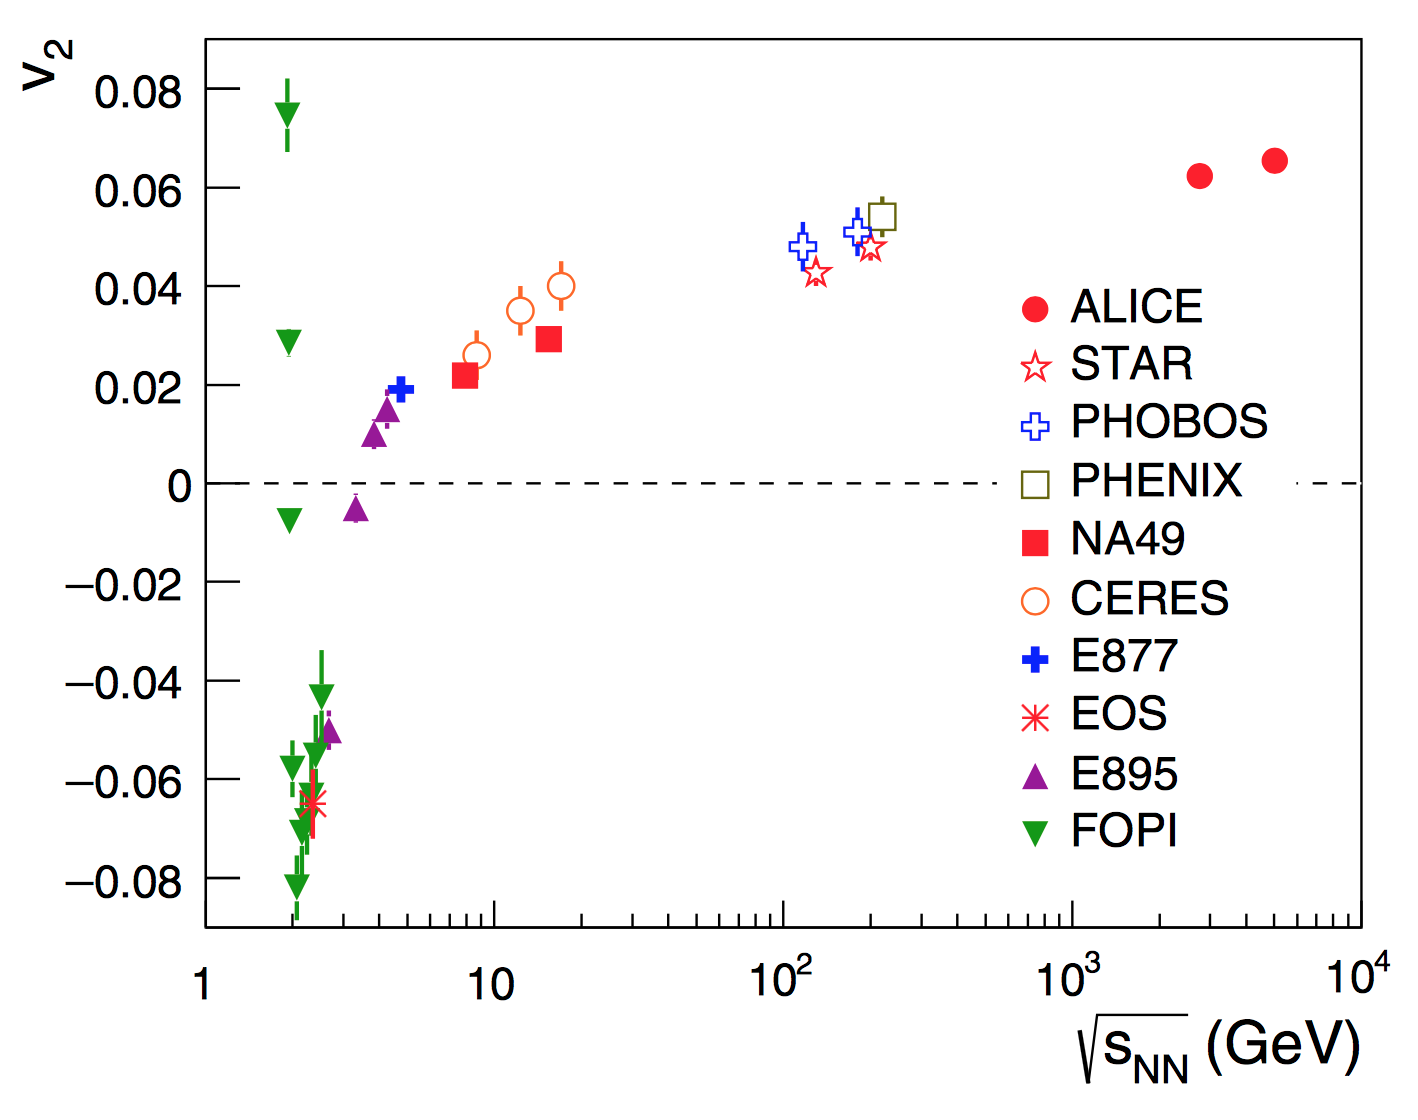
\includegraphics[width=.7\linewidth]{figs/sec_result/energyDep_ALICE.png}
\caption{$v_2$ measured as a function of different collision energies $\sqrt{s_\text{NN}}$, published by ALICE.}
\label{fig:result_energyDep_ALICE}
\end{figure}

ATLAS has measured the $p_\text{T}$ dependence of $c_2\{4\}$ and $c_3\{4\}$ with 2.76 TeV Pb+Pb data~\cite{ATLAS:2014vba}, as shown in Fig.~\ref{fig:result_v2v3_pT_ATLAS}. For $v_2\{2\}$ and higher order cumulants, the magnitude of $v_2$ first increases with $p_\text{T}$, reaches maximum around $2-3$ GeV, then decreases as $p_\text{T}$ goes even higher.
\begin{figure}[H]
\centering
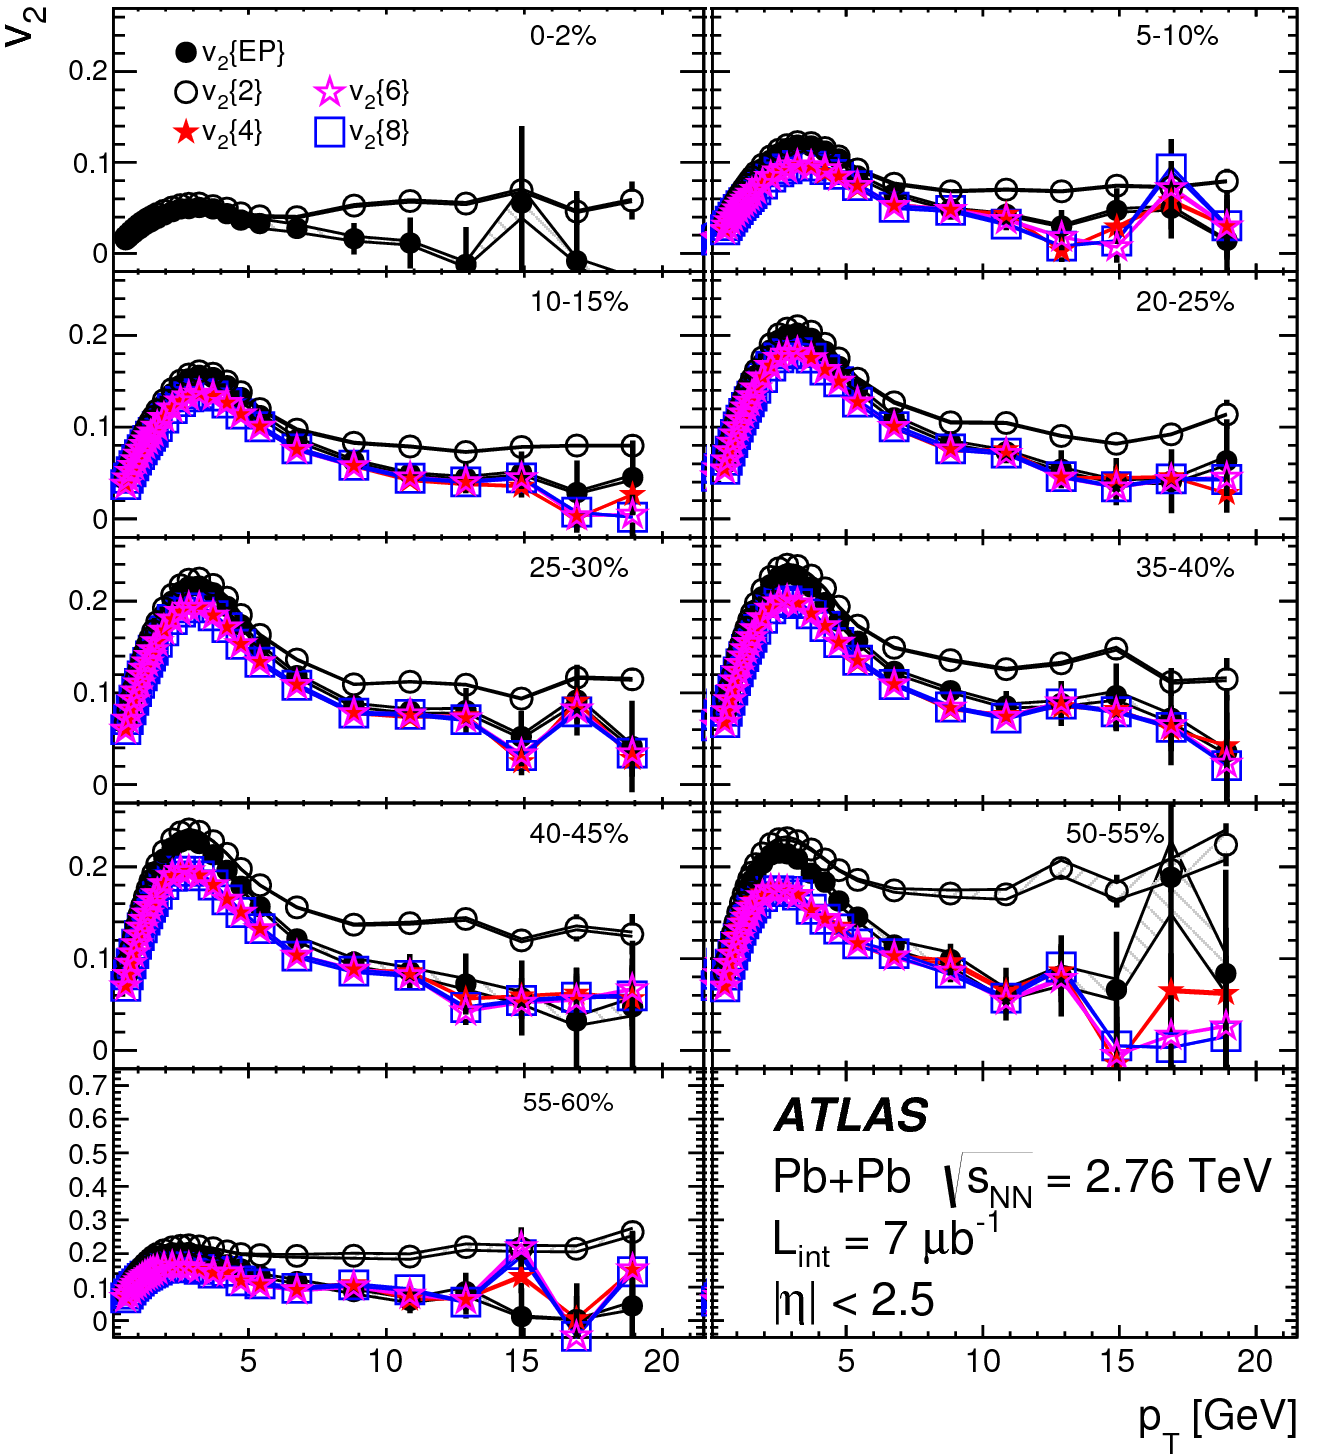
\includegraphics[width=.75\linewidth]{figs/sec_result/v2v3_pT_ATLAS.png}
\caption{$v_2\{2k\}$ measured as a function of $p_\text{T}$, published by ATLAS}
\label{fig:result_v2v3_pT_ATLAS}
\end{figure}

Note that in previous differential multi-particle cumulant measurements~\cite{Aad:2014vba}, $p_\text{T}$ dependence are measured with respect to only one reference particles. While in this analysis, the $p_\text{T}$ dependence are measured with all the particles. For example, to measure cumulant $c_2\{4\}$ in range $2.0<p_\text{T}<5.0$ GeV:
\begin{itemize}
\item Previous differential cumulant: in $\lr{e^{in(\phi_i+\phi_j-\phi_k-\phi_l)}}$, only one particle is from $2.0<p_\text{T}<5.0$ GeV and the rest three particles are from $0.5<p_\text{T}<5.0$ GeV;
\item This analysis: in $\lr{e^{in(\phi_i+\phi_j-\phi_k-\phi_l)}}$, all the four particles are from $2.0<p_\text{T}<5.0$ GeV;
\end{itemize}
The previous differential cumulant measurement assumes that the flow in different $p_\text{T}$ ranges share the same event plane, which might not be the case as shown by the flow decorrelation measurement in $p_\text{T}$~\cite{Khachatryan:2015oea}. Note that there also exists decorrelation in $\eta$~\cite{Aaboud:2017tql}, but in this analysis we are only measuring cumulants as a function of $p_\text{T}$. With Run 2 Pb+Pb data, the statistics are higher, we are correlating all the particles in the selected $p_\text{T}$ range, instead of correlating particles from the low $p_\text{T}$ with high $p_\text{T}$. This will also benefit us in the way that the cumulant formulas are simpler than differential cumulant, without special treatment of reference particles.

For the measurement of $v_1$, a primary background is global momentum conservation (GMC), which induces a significant dipole component. ATLAS has published the 2-particle correlation measurement of $v_1\{2\}$ at 2.76 TeV Pb+Pb~\cite{ATLAS:2012at}, with momentum conservation effects properly removed, as shown in Fig.~\ref{fig:result_v1_pT_ATLAS}. $v_1\{2\}$ as a function of $p_\text{T}$ starts from negative values, and crosses 0 at $p_\text{T}~1$ GeV. It reaches maximum positive at $p_\text{T}~4$ GeV and then decreases towards very high $p_\text{T}$. Different centralities are shown in different panels, and the trends are very similar, meaning a weak centrality dependence of $v_1\{2\}$. Unlike 2-particle correlation, global momentum conservation does not play a role in 4-particle correlation. This is because the 4-particle cumulant is defined as:
\begin{equation}
c_1\{4\} = \lr{v_1^4} - 2\lr{v_1^2}^2
\end{equation}
where GMC contributes to both $\lr{v_1^4}$ and $\lr{v_1}^2$, then most of the effects are canceled.

But in order to obtain a non-zero $c_1\{4\}$ signal, the lowest $p_\text{T}$ cut at least needs to be above 1 GeV. Due to this reason, we have different lowest $p_\text{T}$ cuts from 1.0 GeV to 2.0 GeV.
\begin{figure}[H]
\centering
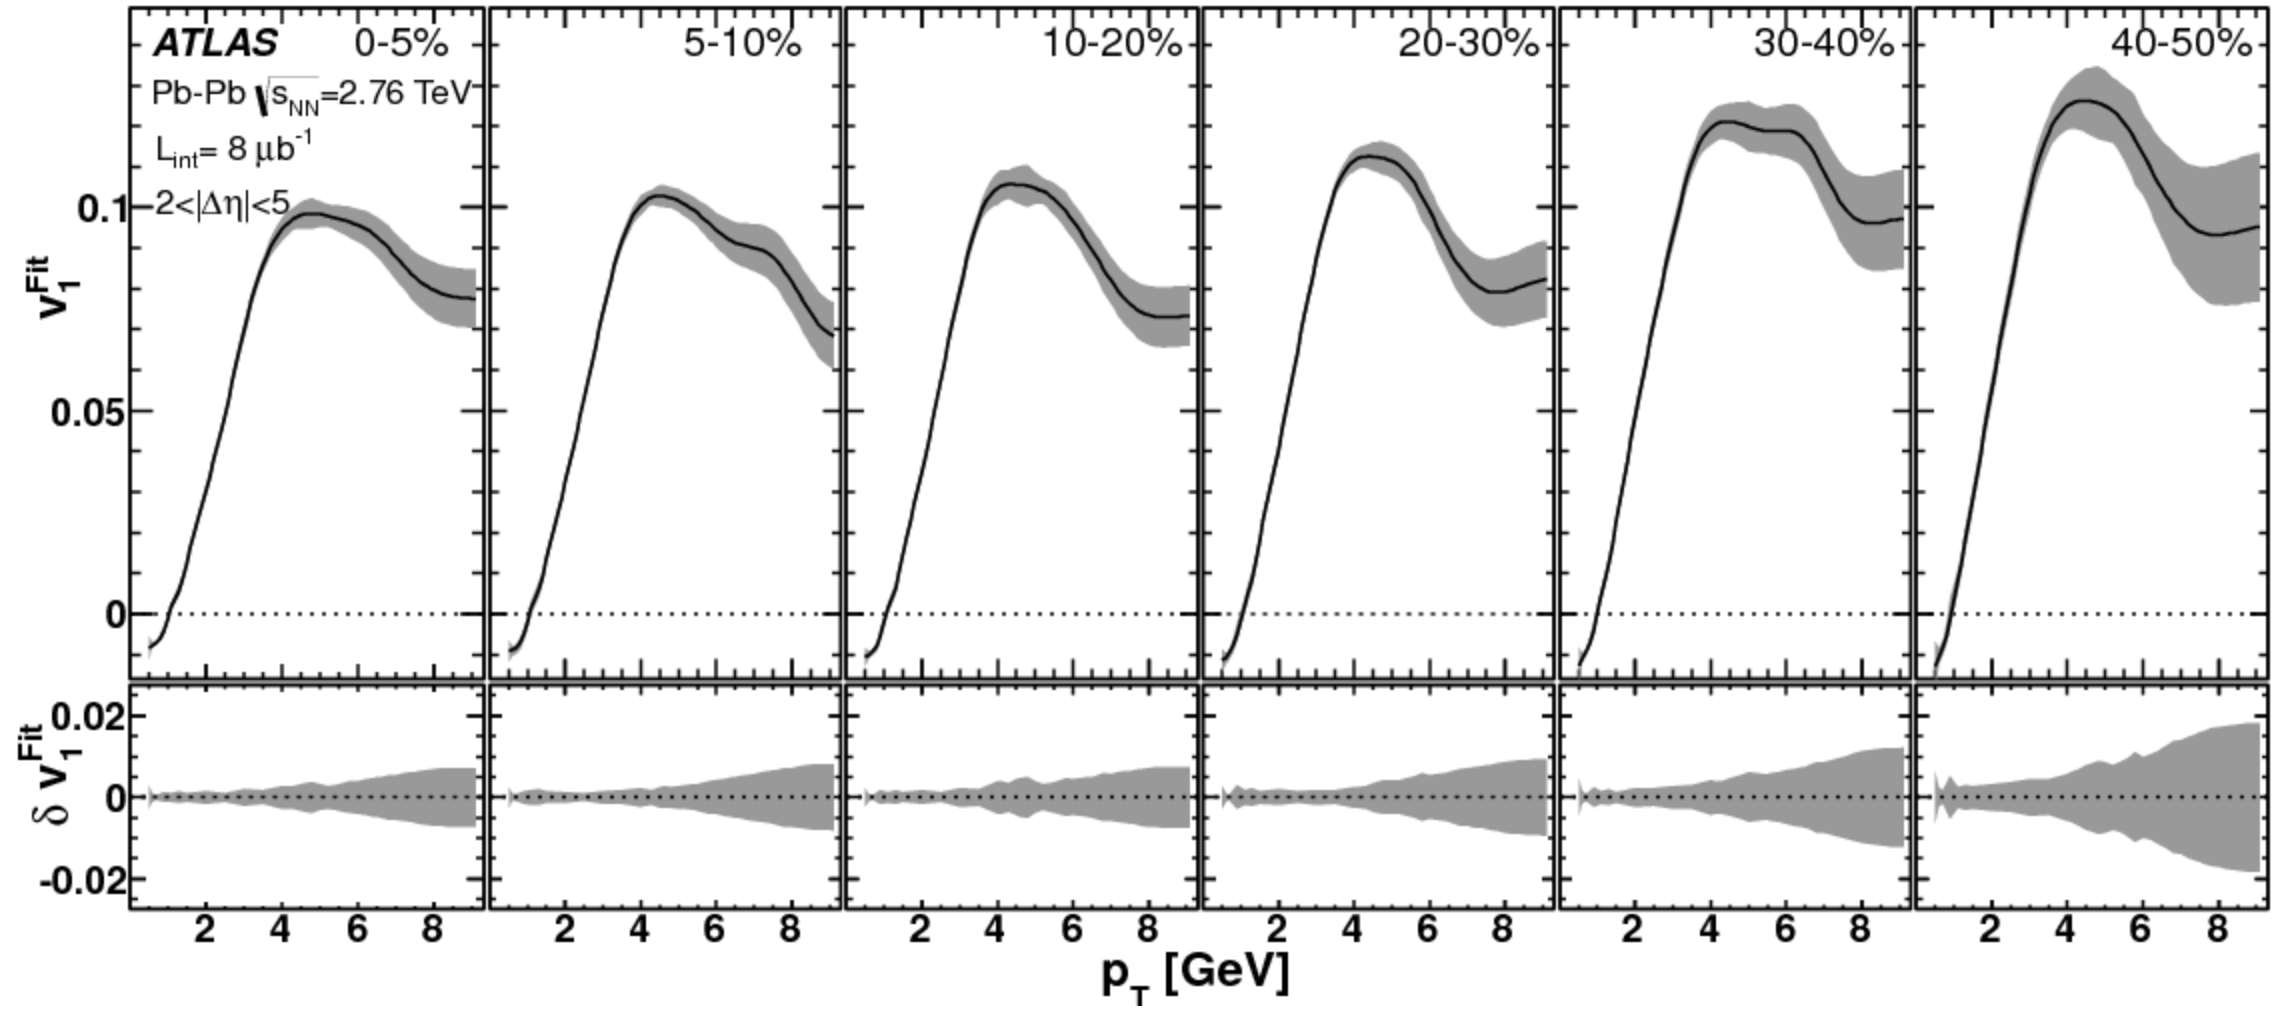
\includegraphics[width=.9\linewidth]{figs/sec_result/v1_pT_ATLAS.png}
\caption{$v_1\{2\}$ measured as a function of $p_\text{T}$, in different centralities, published by ATLAS.}
\label{fig:result_v1_pT_ATLAS}
\end{figure}

Symmetric cumulants, $sc_{n,m}\{4\}$, was first proposed and measured by ALICE~\cite{ALICE:2016kpq}, as shown in Fig.~\ref{fig:result_sc_ALICE}. Symmetric cumulants in HIJING are found to be consistent with 0, meaning that these observables are not sensitive to the non-flow contributions. In this analysis, we have extended the measurements to 5.02 TeV Pb+Pb, with multiple $p_\text{T}$ cuts. Both the energy of $p_\text{T}$ dependence of symmetric cumulants will provide more insights into the flow correlations.
\begin{figure}[H]
\centering
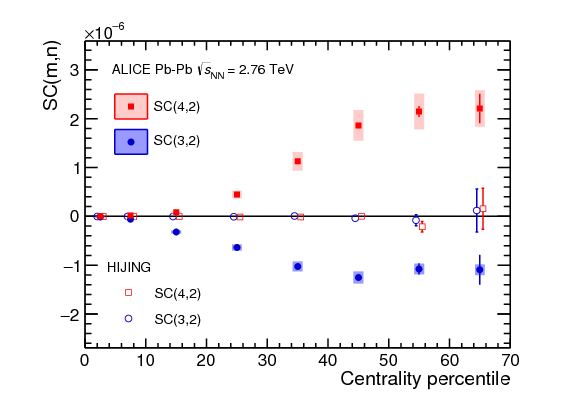
\includegraphics[width=.5\linewidth]{figs/sec_result/sc_ALICE.png}
\caption{Symmetric cumulants $sc_{2,3}\{4\}$ and $sc_{2,4}\{4\}$ as a function of centrality, measured by ALICE.}
\label{fig:result_sc_ALICE}
\end{figure}

Cumulant ratios have long been used to probe the fluctuation of eccentricity $\epsilon_n$ in the initial stage. Recently, CMS collaboration has published the non-Gaussian elliptic-flow fluctuation in 5.02 TeV Pb+Pb~\cite{Sirunyan:2017fts}. In the paper, they measured the cumulant ratio $v_2\{6\}/v_2\{4\}$, as shown in Fig.~\ref{fig:result_cr_CMS}, and the method they used the unfolding technique. In this analysis, we calculated the same observable using multi-particle cumulant. One advantage of cumulant method is that the systematics partially cancels in the ratio, which results in a much better precision. Furthermore, we have tested the non-Gaussian fluctuation in different $p_\text{T}$ ranges, which reflects the additional dynamical fluctuation after the initial stage.
\begin{figure}[H]
\centering
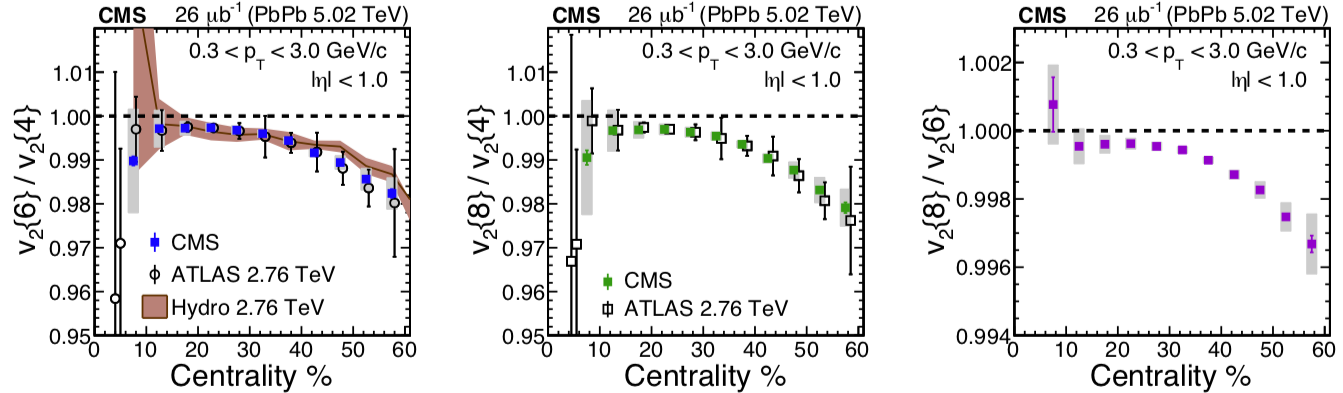
\includegraphics[width=.9\linewidth]{figs/sec_result/cr_CMS.png}
\caption{Cumulant ratio $v_2\{6\}/v_2\{4\}$ as a function of centrality, with unfolding method, published by CMS.}
\label{fig:result_cr_CMS}
\end{figure}








\clearpage

\section{Detector, trigger and offline event selection}
\label{sec:evtSel}
The results presented in this analysis were obtained from a sample of minimum-bias and ultra-central lead-lead collisions at $\sqrt{s_{\text{NN}}}=5.02$ TeV recorded by ATLAS in 2015 (Run 2). The corresponding integrated luminosity are approximated $22-470 \mu b^{-1}$. The measurements were performed using the ATLAS inner detector and forward calorimeters. The inner detectors covers the complete azimuthal range and extends over the pseudorapidity region $|\eta|<2.5$. The inner detector silicon tracker, used in this analysis for track reconstruction, consists of layers of pixel and microstrip detectors (SCT) immersed in a 2 T axial magnetic field. An additional pixel layer, the "Insertable B Layyer" (IBL) installed between Run 1 and Run 2 (2013-2015), is used in the 5.02 TeV Pb+Pb measurements. The MBTS system detects charged particles over $2.1<|\eta|<3.9$ using two hodoscropes of counters positioned at $z=\pm 3.6$ m. The forward calorimeters (FCal) use liquid argon with copper tungsten absorbers to perform both the electromagnetic and hadronic energy measurements with copper-tungsten/liquid argon technology, and also provide complete coverage in azimuthal for $3.2<|\eta|<4.9$. The trigger system was used to select minimum-bias lead-lead collisions. It required a coincidence of signals recorded in both zero-degree calorimeters (ZDC), located symmetrically at $z=\pm 140$ m, and in the minimum-bias trigger scintillator (MBTS, only used in Run 1) counters at $z=\pm 3.6$ m.



\subsection{Triggers}
The minimum-bias triggers for 5.02 TeV Pb+Pb collisions are:
\begin{itemize}
\item \verb|HLT_mb_sptrk_ion_L1ZDC_A_C_VTE50|
\item \verb|HLT_noalg_mb_L1TE50|
\end{itemize}
where the major difference is Level-1 total energy $\verb|TE|$: $\verb|VTE50|$ requires total energy less than 50 GeV while $\verb|TE50|$ larger than 50 GeV; $\verb|sptrk|$ requires at least 1 reconstructed track at the HLT level, and $\verb|L1ZDC_A_C|$ requires one hit in both sides of ZDC. These two requirements will clean up most diffractive events. In any case, this measurement stops at $80\%$ centrality, which means the contributions from diffractive events are minimal.

To enhance the statistics in ultra-central events, ultra-central collision (UCC) triggers are used:
\begin{itemize}
\item \verb|HLT_hi_th1_ucc_L1TE10000|
\item \verb|HLT_hi_th2_ucc_L1TE10000|
\item \verb|HLT_hi_th3_ucc_L1TE10000|
\item \verb|HLT_hi_th1_ucc_L1TE12000|
\item \verb|HLT_hi_th2_ucc_L1TE12000|
\item \verb|HLT_hi_th3_ucc_L1TE12000|
\item \verb|HLT_hi_th1_ucc_L1TE14000|
\item \verb|HLT_hi_th2_ucc_L1TE14000|
\item \verb|HLT_hi_th3_ucc_L1TE14000|
\end{itemize}
where $\verb|L1TEX|$ denotes the minimum L1 total energy cut and $thX$ corresponds to the various minimum FCal Calorimeter $E_{\text{T}}$ cut at the HLT level:
\begin{itemize}
\item \verb|th1|: online FCal $E_{\text{T}}>4.172$ TeV;
\item \verb|th2|: online FCal $E_{\text{T}}>4.326$ TeV;
\item \verb|th3|: online FCal $E_{\text{T}}>4.500$ TeV;
\end{itemize}

Fig.~\ref{fig:evtSel_UCC_sts} shows the FCal $E_{T}$ distributions seeded by two major UCC triggers, compared with those seeded by MinBias triggers. UCC triggers collected more than 20 times statistics compared with MinBias triggers in the ultra-central collisions. Meanwhile, as seen in these plots, the turn-on curves of UCC trigger efficiency are very sharp, which means small selection bias. The impact from trigger efficiency will be discussed in details in Sec.~\ref{sec:sys}.
\begin{figure}[H]
\centering
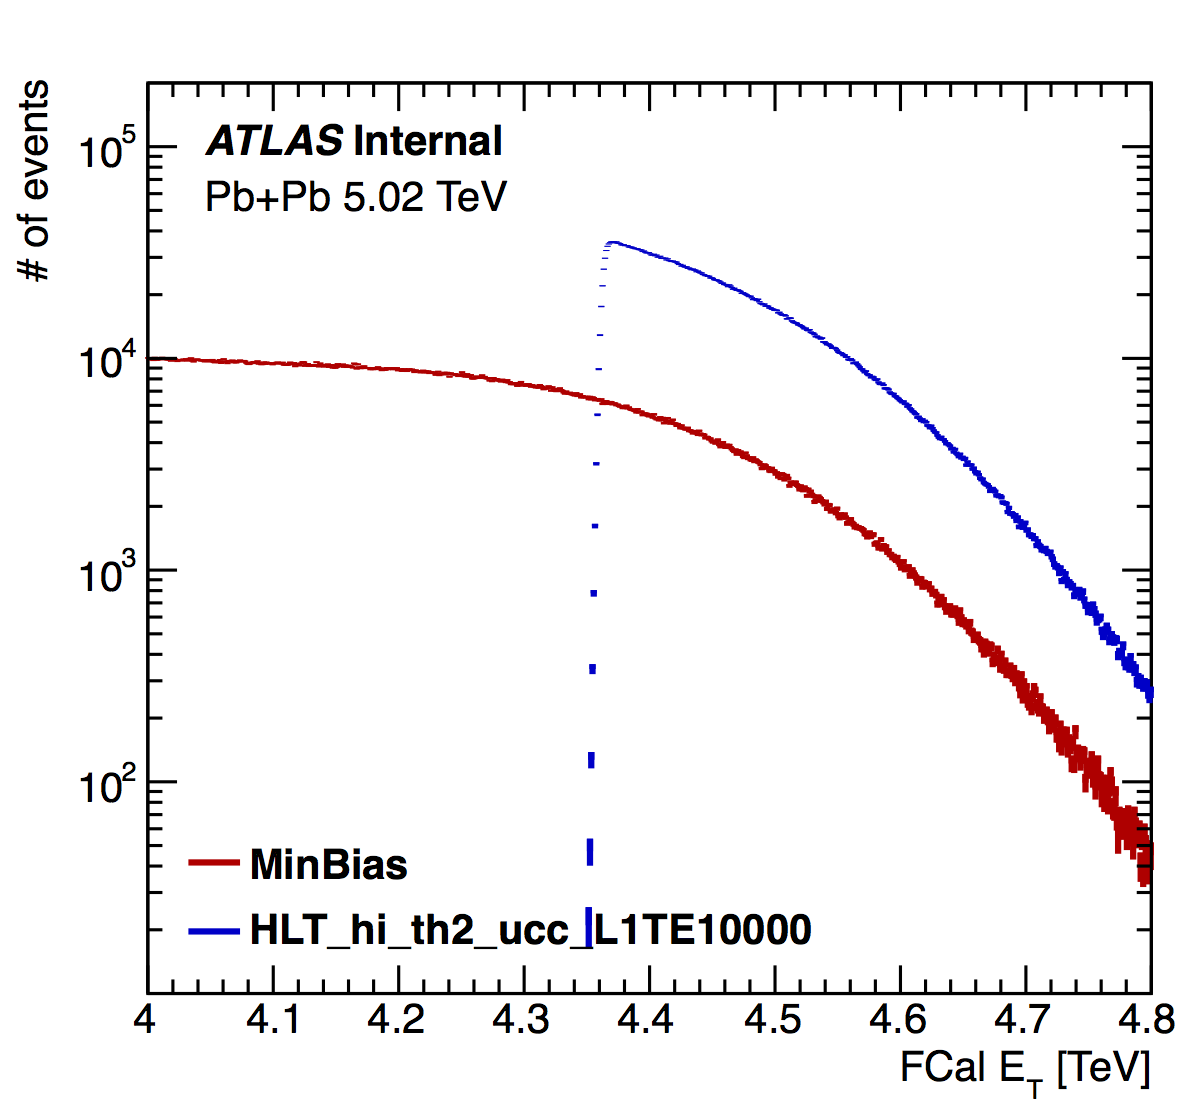
\includegraphics[width=.45\linewidth]{figs/sec_evtSel/PbPb502/UCC_trigSts_3.png}
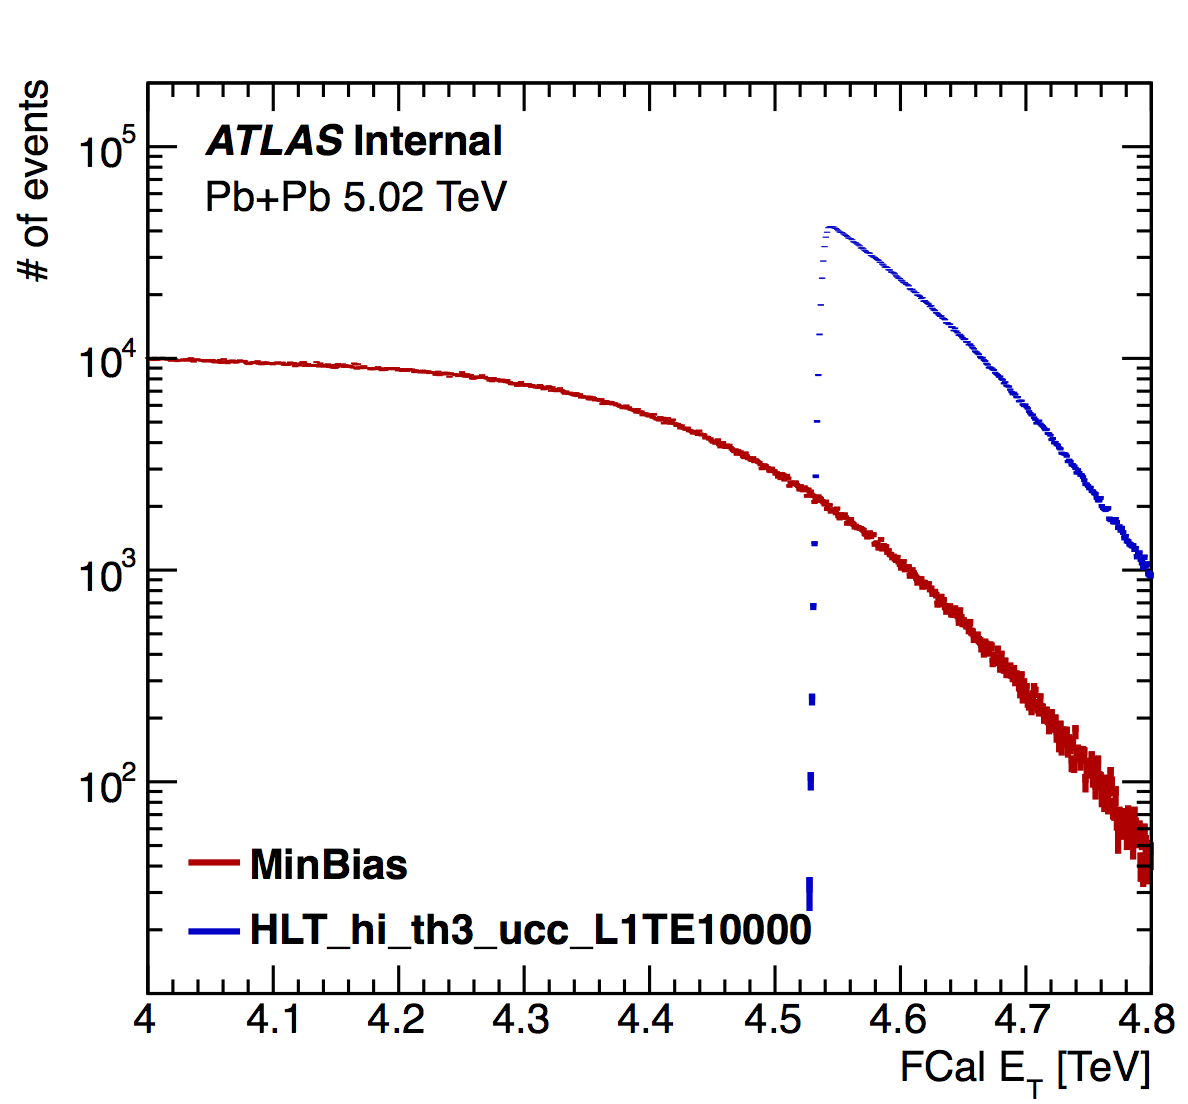
\includegraphics[width=.45\linewidth]{figs/sec_evtSel/PbPb502/UCC_trigSts_4.png}
\caption{FCal $E_{T}$ distribution for two major UCC triggers (red points), compared with MinBias trigger (blue points).}
\label{fig:evtSel_UCC_sts}
\end{figure}



\subsection{Event selection}
The reconstruction version of the data set is $\verb|data15_hi.XXX.physics.MinBias.recon.AOD.r7874|$. The event selections for 5.02 TeV Pb+Pb events are:
\begin{itemize}
\item Pass good run list (GRL): \url{https://twiki.cern.ch/twiki/bin/viewauth/Atlas/HeavyIonRunList};
\item Have a primary reconstructed vertex;
\item Events with detector error tags removed:
\begin{itemize}
\item LAr error;
\item Tile error;
\item SCT error;
\item Incomplete events;
\end{itemize}
\item Vertex position cut: $|z_{vtx}|<100$ mm;
\item $0\%\leq\text{centrality}<80\%$;
\item Pileup rejection: \url{https://twiki.cern.ch/twiki/bin/view/Main/HIAnalysisTools#HI\_Pileup\_Tool\_Working};
\end{itemize}
where the definition of centrality will be discussed shortly. In this analysis we are cutting the vertex position at $100$ mm instead of $150$ mm (in previous Pb+Pb analysis). This is because multiplicity distribution along $\eta$ changes with the $z_{vtx}$ position, and in previous measurements it is not an issue since all the particles in $|\eta|<2.5$ are used to calculate the cumulant. However, with the 3-subevent cumulant method, two subevents are defined with the range $2.5/3<|eta|<2.5$, which is closer to the edges of the Inner Detector. In order to avoid introducing large multiplicity fluctuations in these two subevents, we further constrain the vertex position to $100$ mm, and we will not loose much statistics with this tighter cut.

In the 2015 Pb+Pb run, the luminosity conditions provided by the LHC result in an average probability of $0.1\%$ that an event contains two or more Pb+Pb collisions (pileup). The pileup events are suppressed by only using the tracks from primary vertex (in fact, in Pb+Pb, only one primary vertex is reconstructed). The remaining pileup events are further suppressed based on the correlation between the ZDC and FCal. This signal in the ZDC is calibrated to the number of detected neutrons $N_n$ based on the location of the peak corresponding to a single neutron.

Fig.~\ref{fig:evtSel_pu} shows the procedure of pileup rejection and its performance. The left plot shows the correlation between number of neutrons in the ZDC and total transverse energy $E_T$ in the FCal. The "banana"-shaped main band (green) mainly contains events with a single vertex. While in a pileup event, both the number of neutrons and FCal $\sum E_T$ are larger than a single event, and this is indicated by the events in the "grass" (purple) region above the main band. To clean up the pileup, one way is by applying a linear cut on the correlation map, indicated by the black straight line, and another way is cutting off $0.1\%$ of the events in the tails of $N_\text{neutrons}$ distribution in each FCal $E_{T}$ slice, indicated by the red curve. In this analysis, we will use the red curve as the default cut. The right plot shows the performance of the two pileup rejection methods just mentioned. The Y-axis shows the fraction of rejected pileup events out of all the pileup events. The rejection rate is low at low FCal $E_{T}$, this is because the band for pileup events most overlaps with the main band for single events. However, since the fraction of pileup events is very low in peripheral collisions, the low rejection rate has no impact on the results. On the other hand, the rejection rate reaches $100\%$ in ultra-central collision, where the fraction of pileup event is high, meaning that almost all the pileup events are rejected using the HI pileup rejection tool.
\begin{figure}[H]
\centering
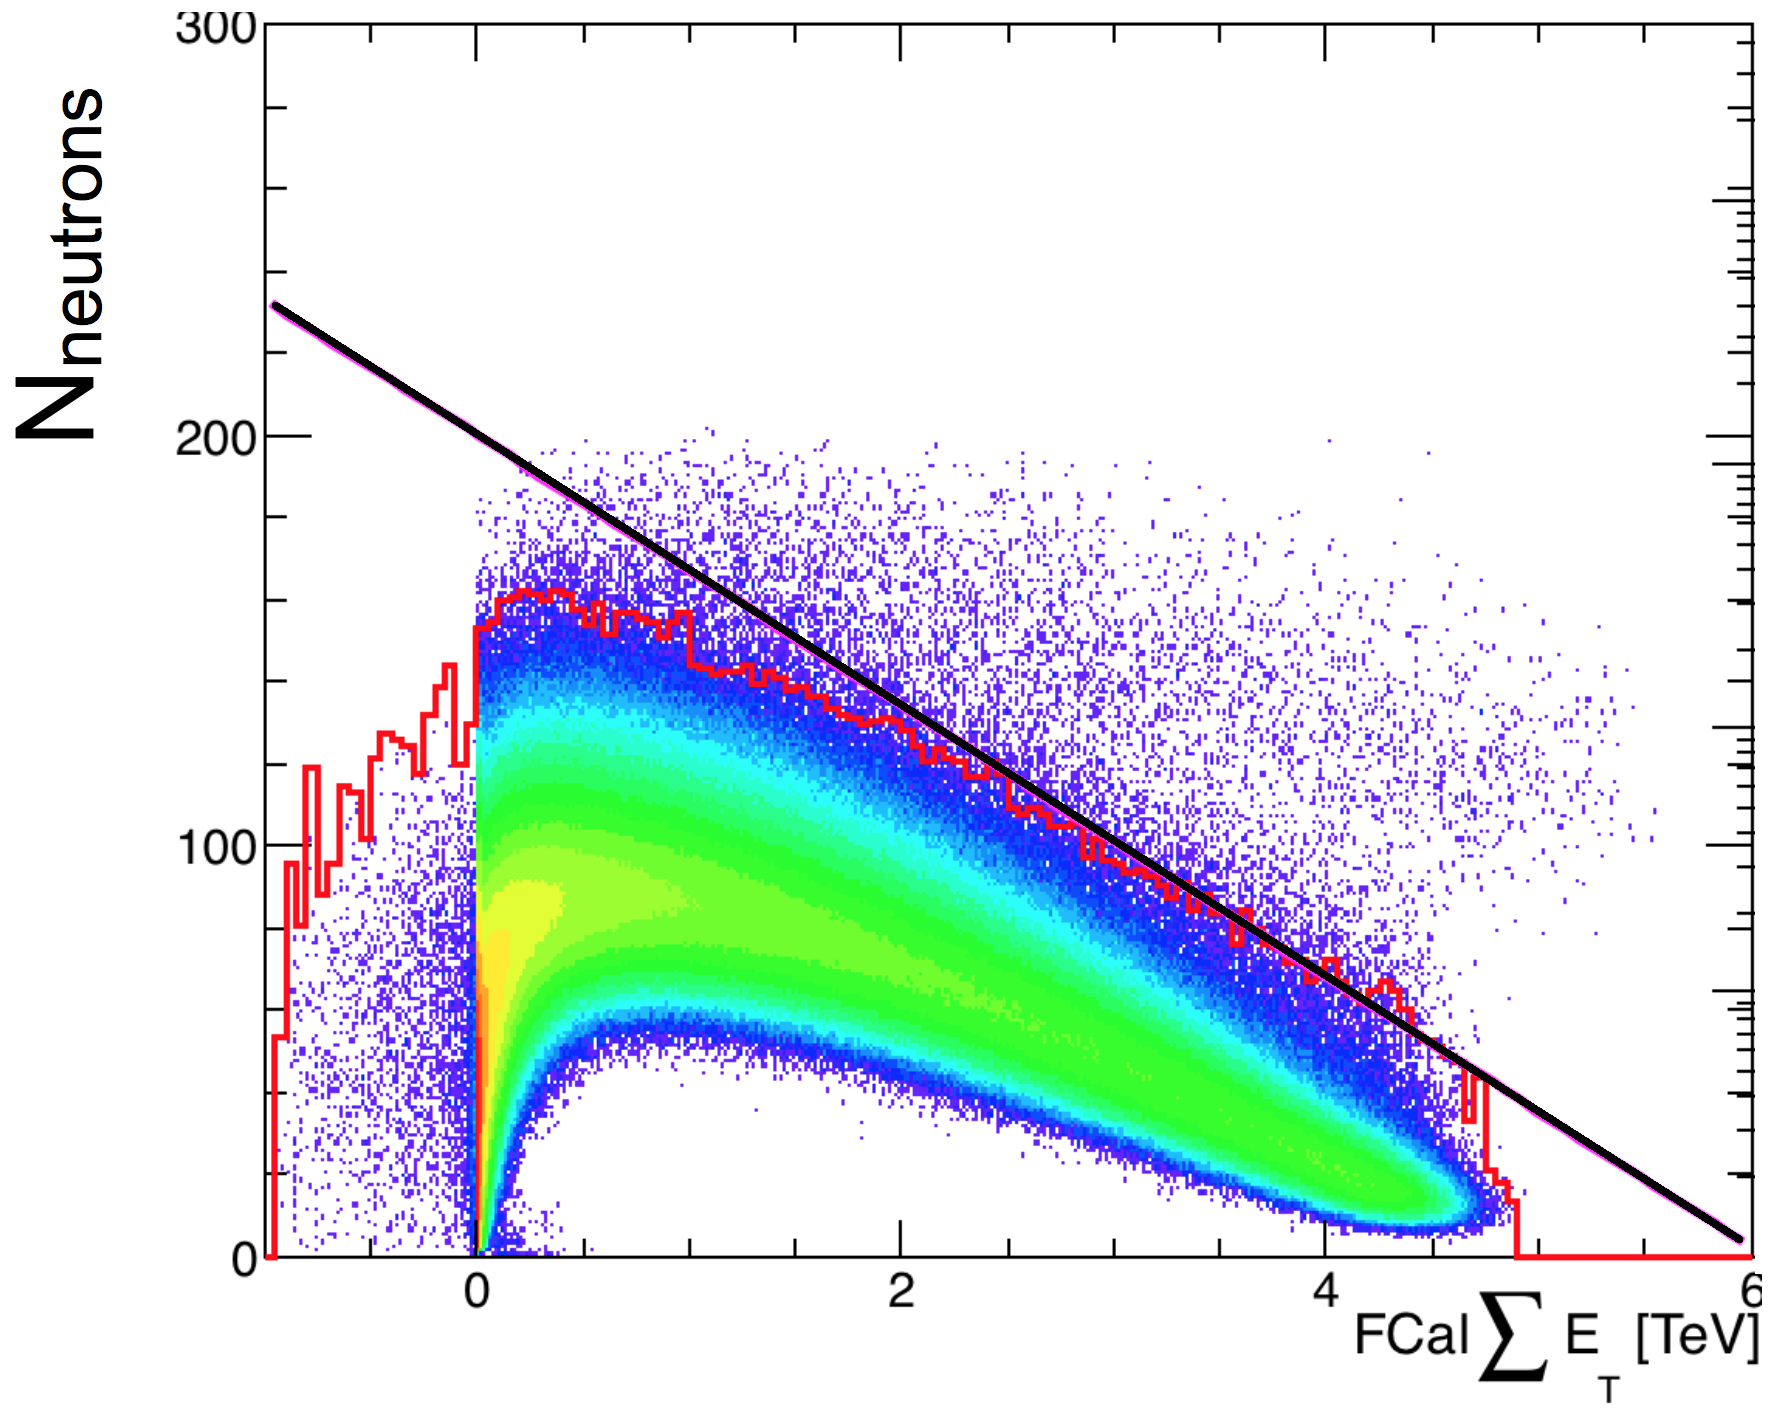
\includegraphics[width=.45\linewidth]{figs/sec_evtSel/PbPb502/pu_corr.png}
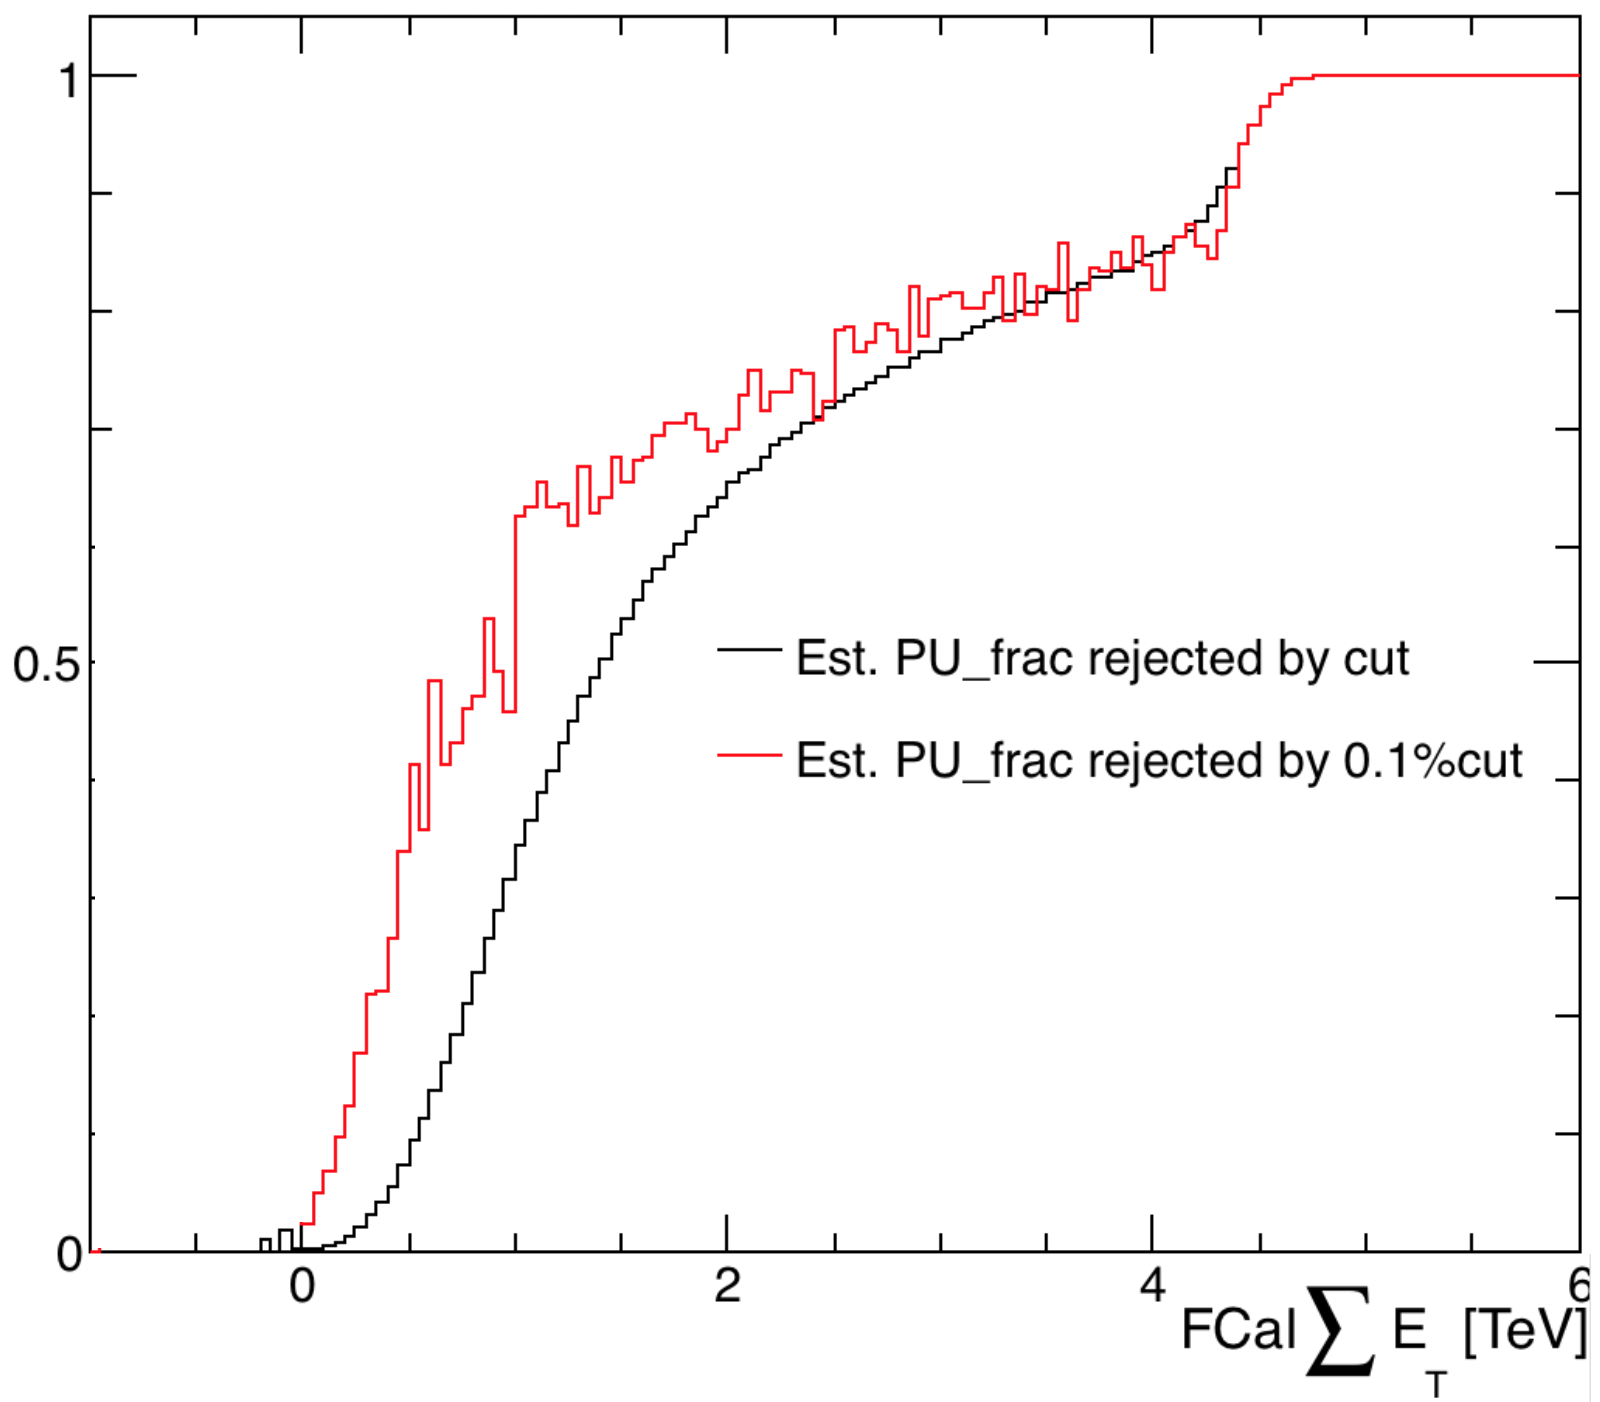
\includegraphics[width=.45\linewidth]{figs/sec_evtSel/PbPb502/pu_perf.png}
\caption{Left plot shows the correlation between calibrated number of neutrons in the ZDC and FCal $\sum E_T$. Right plot shows the fraction of rejected pileup events in all pileup events. Two rejection criteria are shown: a linear cut and $0.1\%$ cut.}
\label{fig:evtSel_pu}
\end{figure}

Fig.~\ref{fig:evtSel_pu_rate} illustrates the FCal sum $E_T$ distribution before and after this pileup cut, as well as the fraction of events that are rejected as a function of FCal sum $E_T$. As expected, the rejection rate is $<0.2\%$ for FCal $E_T<4.5$ TeV, and increases toward 1 quickly as FCal $E_T$ increases.
\begin{figure}[H]
\centering
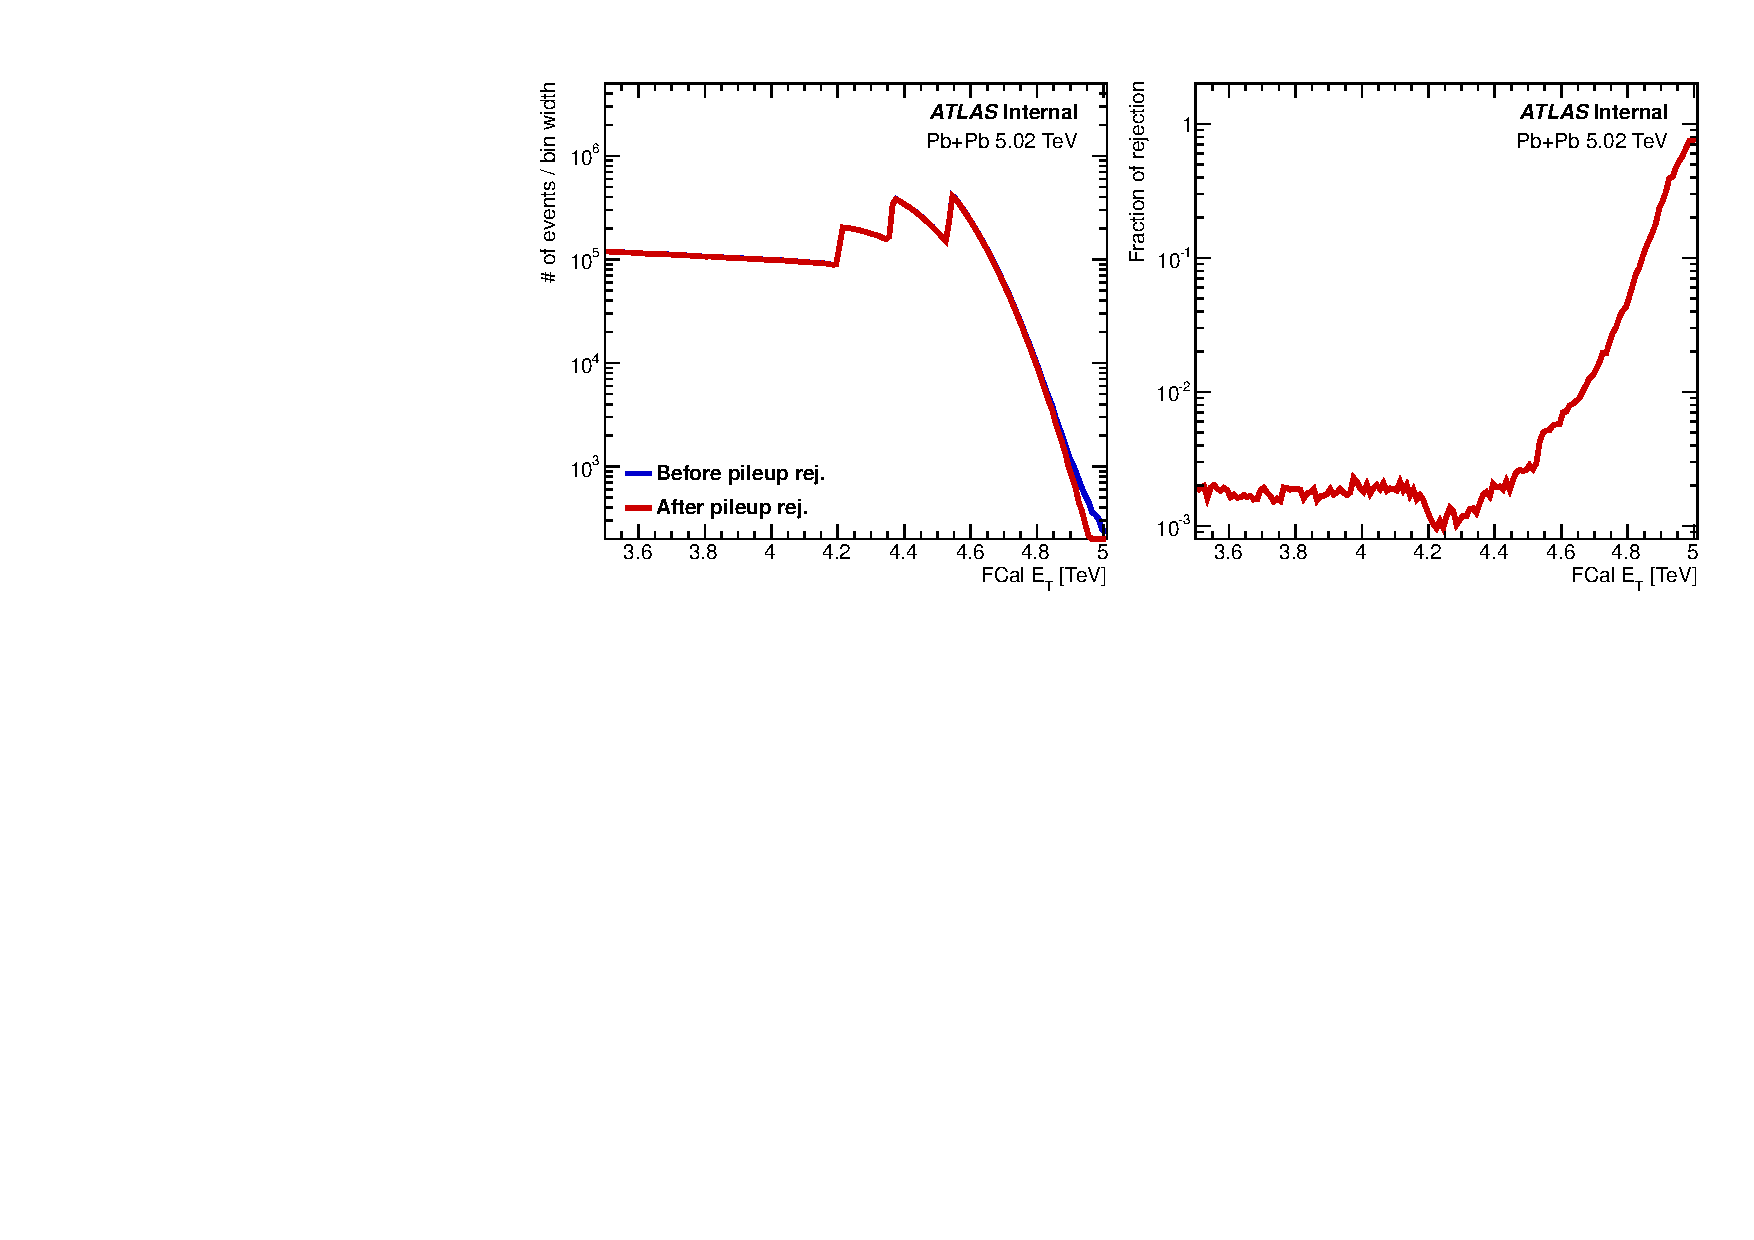
\includegraphics[width=.9\linewidth]{figs/sec_evtSel/PbPb502/puCut.pdf}
\caption{Left plot shows the FCal sum $E_T$ distribution before and after applying the HI pileup tool. Right plot shows the fraction of events that are rejected by this tool, as a function of FCal sum $E_T$.}
\label{fig:evtSel_pu_rate}
\end{figure}

Furthermore, in order to further suppress the residual pileup events, an additional cut has been applied on the correlation map between FCal $E_{T}$ and efficiency corrected reconstructed number of tracks $N_{ch}$. Fig.~\ref{fig:evtSel_addPuCut} shows the correlation froms MinBias events (left), and UCC events collected with one of the UCC triggers (right) as a demonstration. Since pileup events have relatively larger FCal $E_{T}$ than normal events, the pileup events should fall under the main correlation band. From the correlation map, some "grass" is indeed observed. To determine the cut, a Gaussian fitting is applied to the $N_{ch}$ distribution for each FCal $E_{T}$ slice, and the events beyond $5 \sigma$ are rejected (indicated by the red dots). To reach the high FCal $E_{T}$ region, where the performance of Gaussian fit is poor (because of the additional structure from pileup events), a linear cut is determined by fitting the red dots in the region FCal $E_\text{T}<4,7$ TeV. Events below this linear cut are rejected.
\begin{figure}[H]
\centering
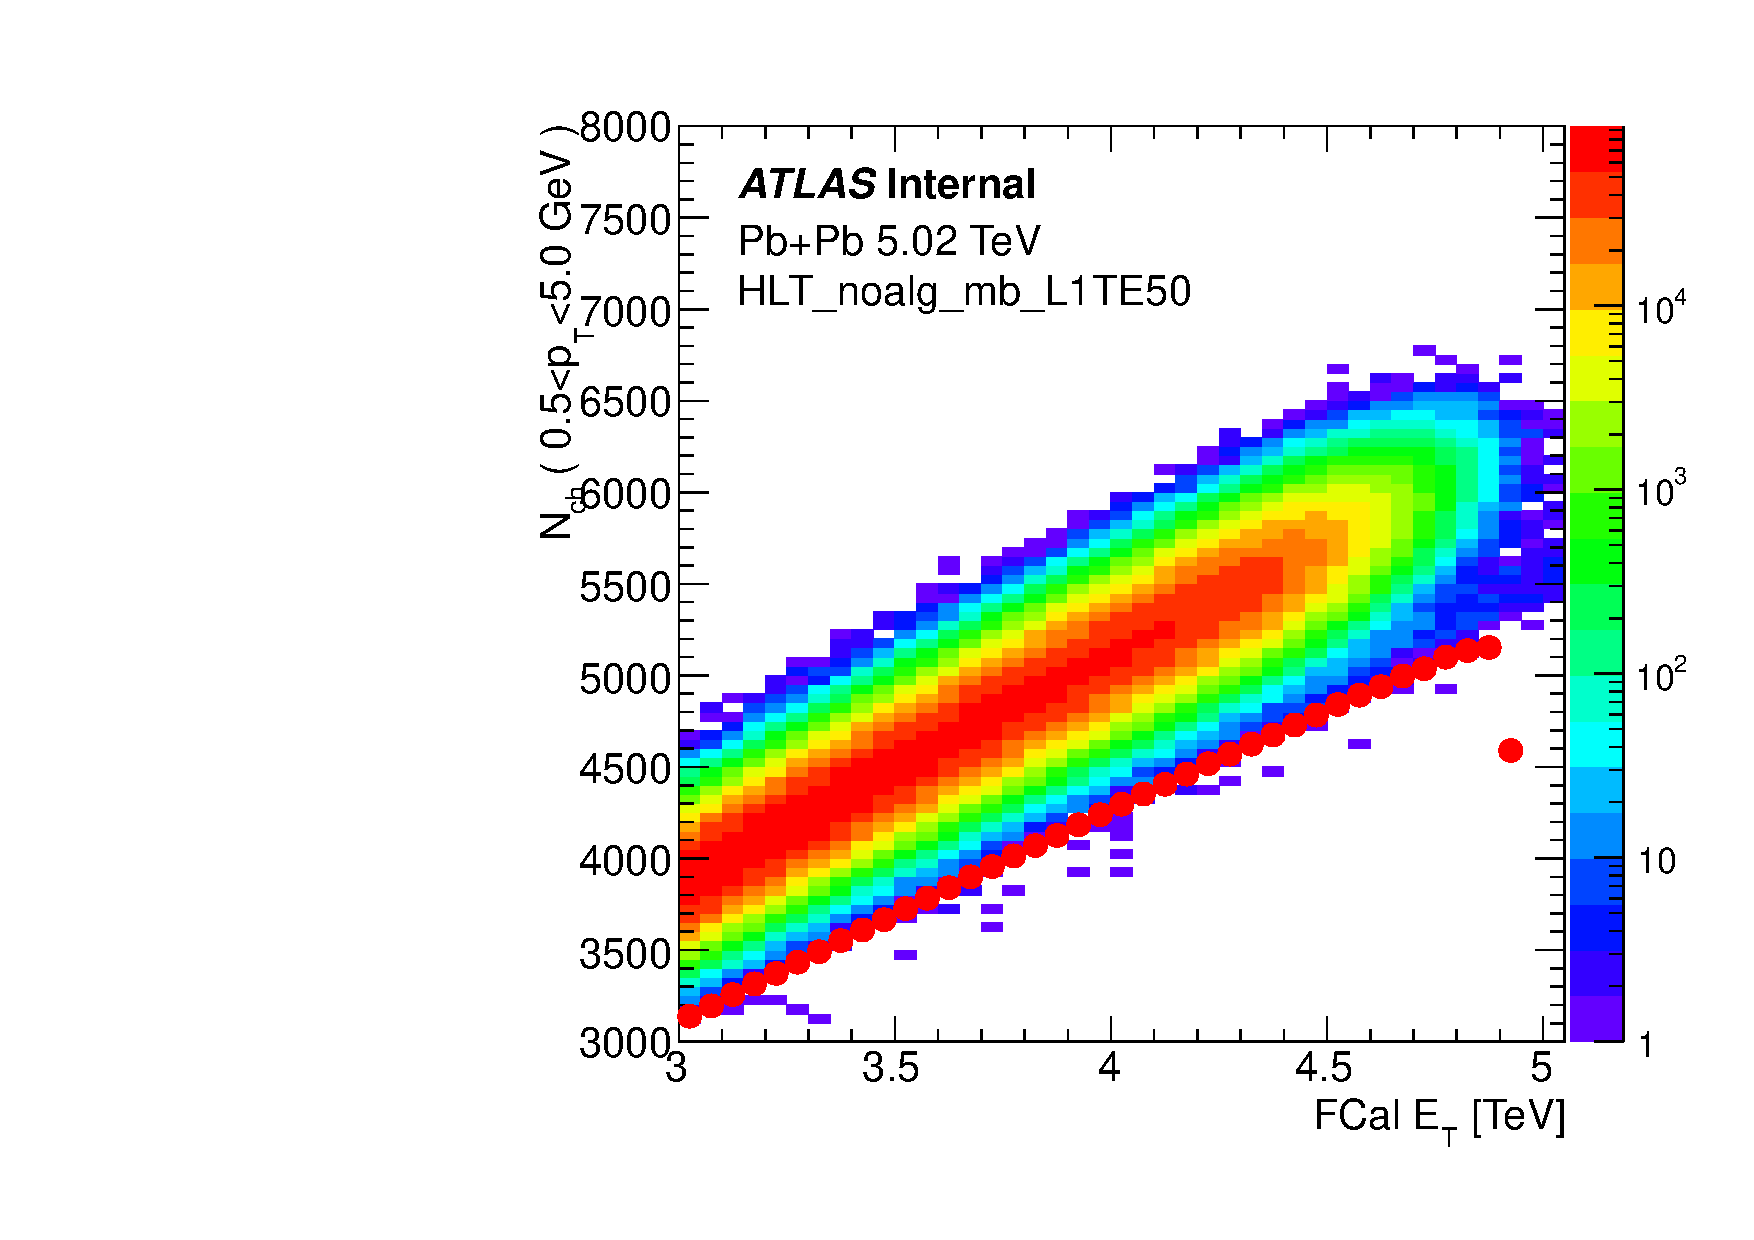
\includegraphics[width=.45\linewidth]{figs/sec_evtSel/PbPb502/puCut_1.pdf}
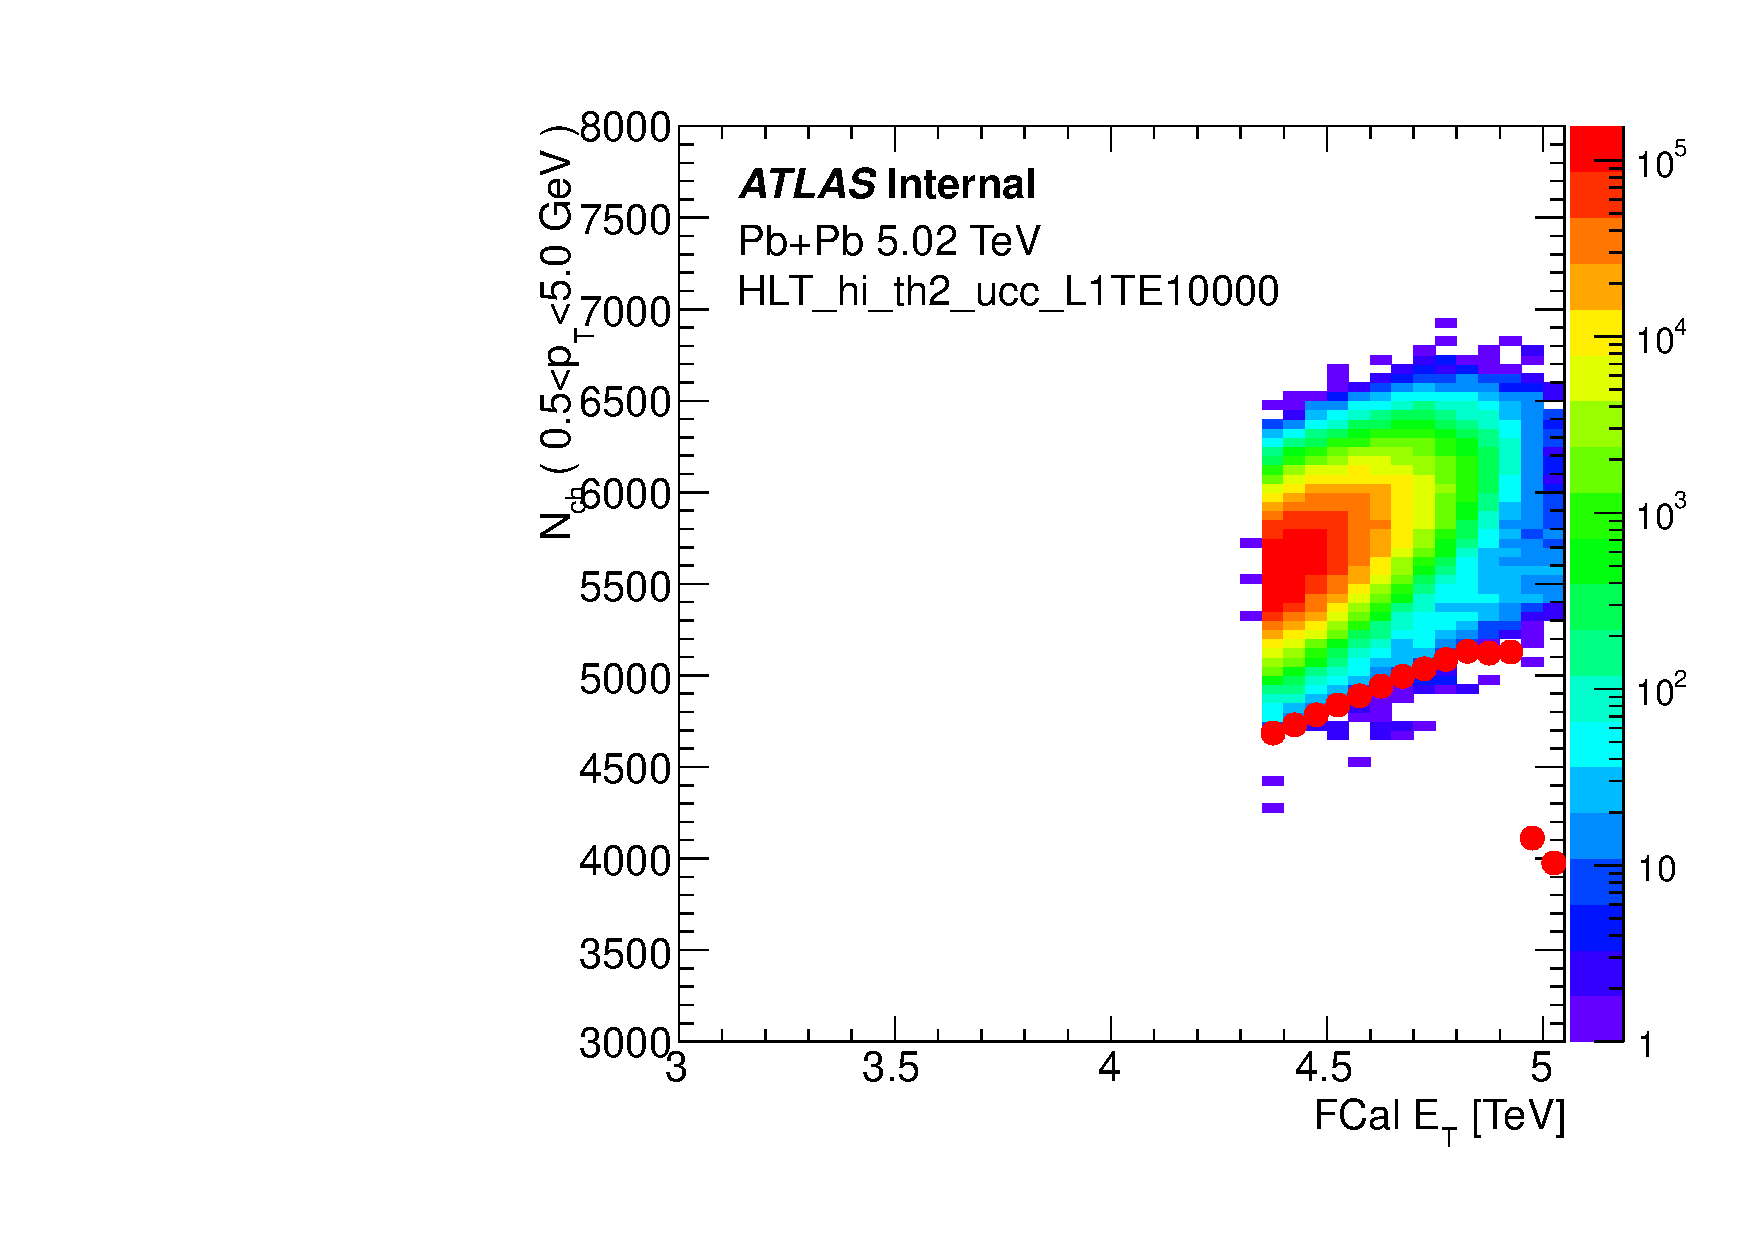
\includegraphics[width=.45\linewidth]{figs/sec_evtSel/PbPb502/puCut_3.pdf}
\caption{Correlation between FCal $E_{T}$ and $N_{ch}$ in the ultra-central collisions. The red dots indicate the $5 \sigma$ position of the Gaussian fit in each $N_{ch}$ slice at fixed FCal $E_{T}$. The actual cut is a linear fit of the red points in order to reach the largest FCal $\sum E_T$ region.}
\label{fig:evtSel_addPuCut}
\end{figure}



\subsection{Centrality}
The details of centrality cuts are documented here: \url{https://twiki.cern.ch/twiki/bin/view/AtlasProtected/HeavyIonAnalysis2015#NEW\_Centrality\_Recommendations\_f}. The Pb+Pb event centrality is characterized using the total transverse energy ($\sum E_T$) deposited in the FCal detector at the electromagnetic energy scale. An analysis of this distribution after all triggers and event selections gives an estimation of the fraction of the sampled non-Coulomb inelastic cross-section to be $85\%\pm1\%$. This estimate is obtained from a shape analysis of the measured FCal $\sum E_T$ distributions compared with a convolution of proton-proton data with a Monte Carlo Glauber calculation. The FCal $\sum E_T$ distribution is then divided into a set of $1\%$ percentile bins, together with a bin defined for the $0.1\%$ most central events. The uncertainty associated with the centrality definition is evaluated by varying the effect of trigger and event selection inefficiencies as well as background rejection requirements in the most peripheral FCal $\sum E_T$ interval.

The centrality interval and corresponding number of participants $N_{\text{part}}$ estimated from Glauber model are listed in Table.~\ref{table:centrality_run2}
\begin{table}[ht]
\begin{tabular}{c c c c c c c c c}
\hline\hline
Centrality        &  0-5\% & 5-10\% & 10-15\% & 15-20\% & 20-25\% & 25-30\% & 30-35\% & 35-40\% \\
$N_{\text{part}}$ &  384.5 & 333.1  & 285.2   & 242.9   & 205.6   & 172.8   & 144.1   & 118.8   \\
Centrality        &40-45\% & 45-50\%& 50-55\% & 55-60\% & 60-65\% & 65-70\%  & 70-75\%& 75-80\% \\ 
$N_{\text{part}}$ &96.6    & 77.4    & 60.9    & 47.0    & 35.2    & 25.8     & 18.3   & 12.5 \\
\hline
\end{tabular}
\centering
\caption{Centrality intervals and corresponding number of participants $N_{\text{part}}$ estimated from Glauber model in Run 2.}
\label{table:centrality_run2}
\end{table}


\clearpage

\section{Track selection, efficiency and fakes}
\label{sec:trkSel}
\subsection{Track selection}
The track selection for 5.02 TeV Pb+Pb follows the standard cut implemented in the $\verb|xAOD ToolInDet|$:

Loose quality cut is denoted as $\verb|HILoose|$ and is defined as:
\begin{itemize}
\item $p_{\text{T}}>500$ MeV;
\item number of Pixel hits $>0$;
\item number of SCT hits + dead sensors $\geq 6$;
\item if IBL hit is expected: at least 1 IBL hit required;
\item if no IBL hit is expected: a Layer-0 hit if expected;
\item $|d_0|\leq 1.5$ mm;
\item $|z_0-z_{\text{vtx}}|*\text{sin}\theta\leq 1.5$ mm;
\end{itemize}
where "ndf" denotes number of degree of freedom of the track.

Tight quality cut is denoted as $\verb|HITight|$ and is defined as:
\begin{itemize}
\item $p_{\text{T}}>500$ MeV;
\item *** number of Pixel hits $>1$;
\item *** number of SCT hits + dead sensors $\geq 8$;
\item if IBL hit is expected: at least 1 IBL hit required;
\item if no IBL hit is expected: a Layer-0 hit if expected;
\item *** $|d_0|\leq 1.0$ mm;
\item *** $|z_0-z_{\text{vtx}}|*\text{sin}\theta\leq 1.0$ mm;
\item *** $\chi^2/\text{ndf}\leq 6$;
\end{itemize}
where the differences compared with loose cut are highlighted with "***". In this analysis, the default track selection is the loose quality cut, and tight quality cut is used as a systematic check and is discussed in Section.~\ref{sec:sys}. We prefer $\verb|HILOOSE|$ over $\verb|HITIGHT|$ mainly because there are more particles remaining with the loose cut, which results in smaller statistical uncertainties. The loose and tight cuts are determined by evaluating the tracking efficiency and fake rates in the Monte-Carlo samples with same detector conditions as during the data taking and these two cuts results in relatively lower fake rates with high tracking efficiency.



\subsection{Tracking in Monte-Carlo}
To estimate the tracking efficiency and fake rate in 5.02 TeV Pb+Pb, HIJING Monte-Carlo samples with similar detector conditions and flow after-burner~\cite{Poskanzer:1998yz} are used:
\begin{itemize}
\item \verb|mc15_5TeV.420000.Hijing_PbPb_5p02TeV_MinBias_Flow_JJFV6.recon.AOD.| \\
\verb|e4962_a868_s2921_r9447|
\end{itemize}

Within the reconstructed tracks, the primary tracks $N_{ch}^{primary}$ are defined as:
\begin{itemize}
\item pass the loose track quality selection;
\item truth match probability $> 0.5$;
\item associated truth particle is a primary particle;
\end{itemize}
where primary particle is defined on the truth level:
\begin{itemize}
\item status $= 1$, charge $!= 0$;
\item $p_{\text{T}}>200$ MeV;
\item $|\eta|\leq 2.5$;
\item $0 < \text{Barcode} < 2\text{E}5$;
\item strange baryons are excluded;
\end{itemize}

The tracking efficiency $\epsilon$ is then defined as:
\begin{equation}
\epsilon(p_{\text{T}},\eta,\text{centrality})\equiv \frac{N_{ch}^{primary}}{N_{ch}^{truth}}
\end{equation}
where $N_{ch}^{primary}$ denotes the number of primary tracks on reconstructed level and $N_{ch}^{truth}$ denotes the number of primary particles on the truth level, all of which passed the loose quality selection.

The fake track is defined as:
\begin{itemize}
\item pass the loose track quality selection;
\item fulfill one of the following:
\begin{itemize}
\item truth match probability $< 0.5$;
\item not associated with truth particles;
\item Barcode $= 0$ of associated truth particle;
\end{itemize}
\end{itemize}

The fraction of fake tracks $f$ is defined as:
\begin{equation}
f(p_{\text{T}},\eta,\text{centrality})\equiv \frac{N_{ch}^{fake}}{N_{ch}^{primary}+N_{ch}^{fake}}
\end{equation}
where $N_{ch}^{fake}$ denotes the number of fake tracks.

To compensate the contribution from fake tracks, the efficiency $\epsilon$ can be corrected by defining $\epsilon^{'}$:
\begin{equation}
\epsilon^{'}(p_{\text{T}},\eta,\text{centrality})\equiv \frac{N_{ch}^{primary}+N_{ch}^{fake}}{N_{ch}^{truth}}=\frac{\epsilon}{1-f}
\end{equation}
where an additional correction of fake rates $1-f$ is added to the tracking efficiency $\epsilon$.



\subsection{Efficiency}
The tracking efficiency map used in this analysis is borrowed from Run 2 $v_n$ analysis~\cite{Burka:2151932}, which is evaluated as a function of $p_{\text{T}}, \eta$ and centrality. To estimate the tracking efficiency, the track selection follows the loose quality cut. The tracking efficiency $\epsilon(\eta)$ are shown in Fig.~\ref{fig:PbPb502_trkEff}, for different $p_{\text{T}}$ ranges and centrality. $\epsilon(\eta)$ is highest in mid-rapidity $-1<\eta<1$, and decreases by $~20\%$ in forward-rapidity. As collision moves to peripheral, the efficiency increases. The tracking efficiency slightly increases towards higher $p_{\text{T}}$. Efficiency from $\verb|HILOOSE|$ is higher than $\verb|HITIGHT|$ as expected.
\begin{figure} [H]
\centering
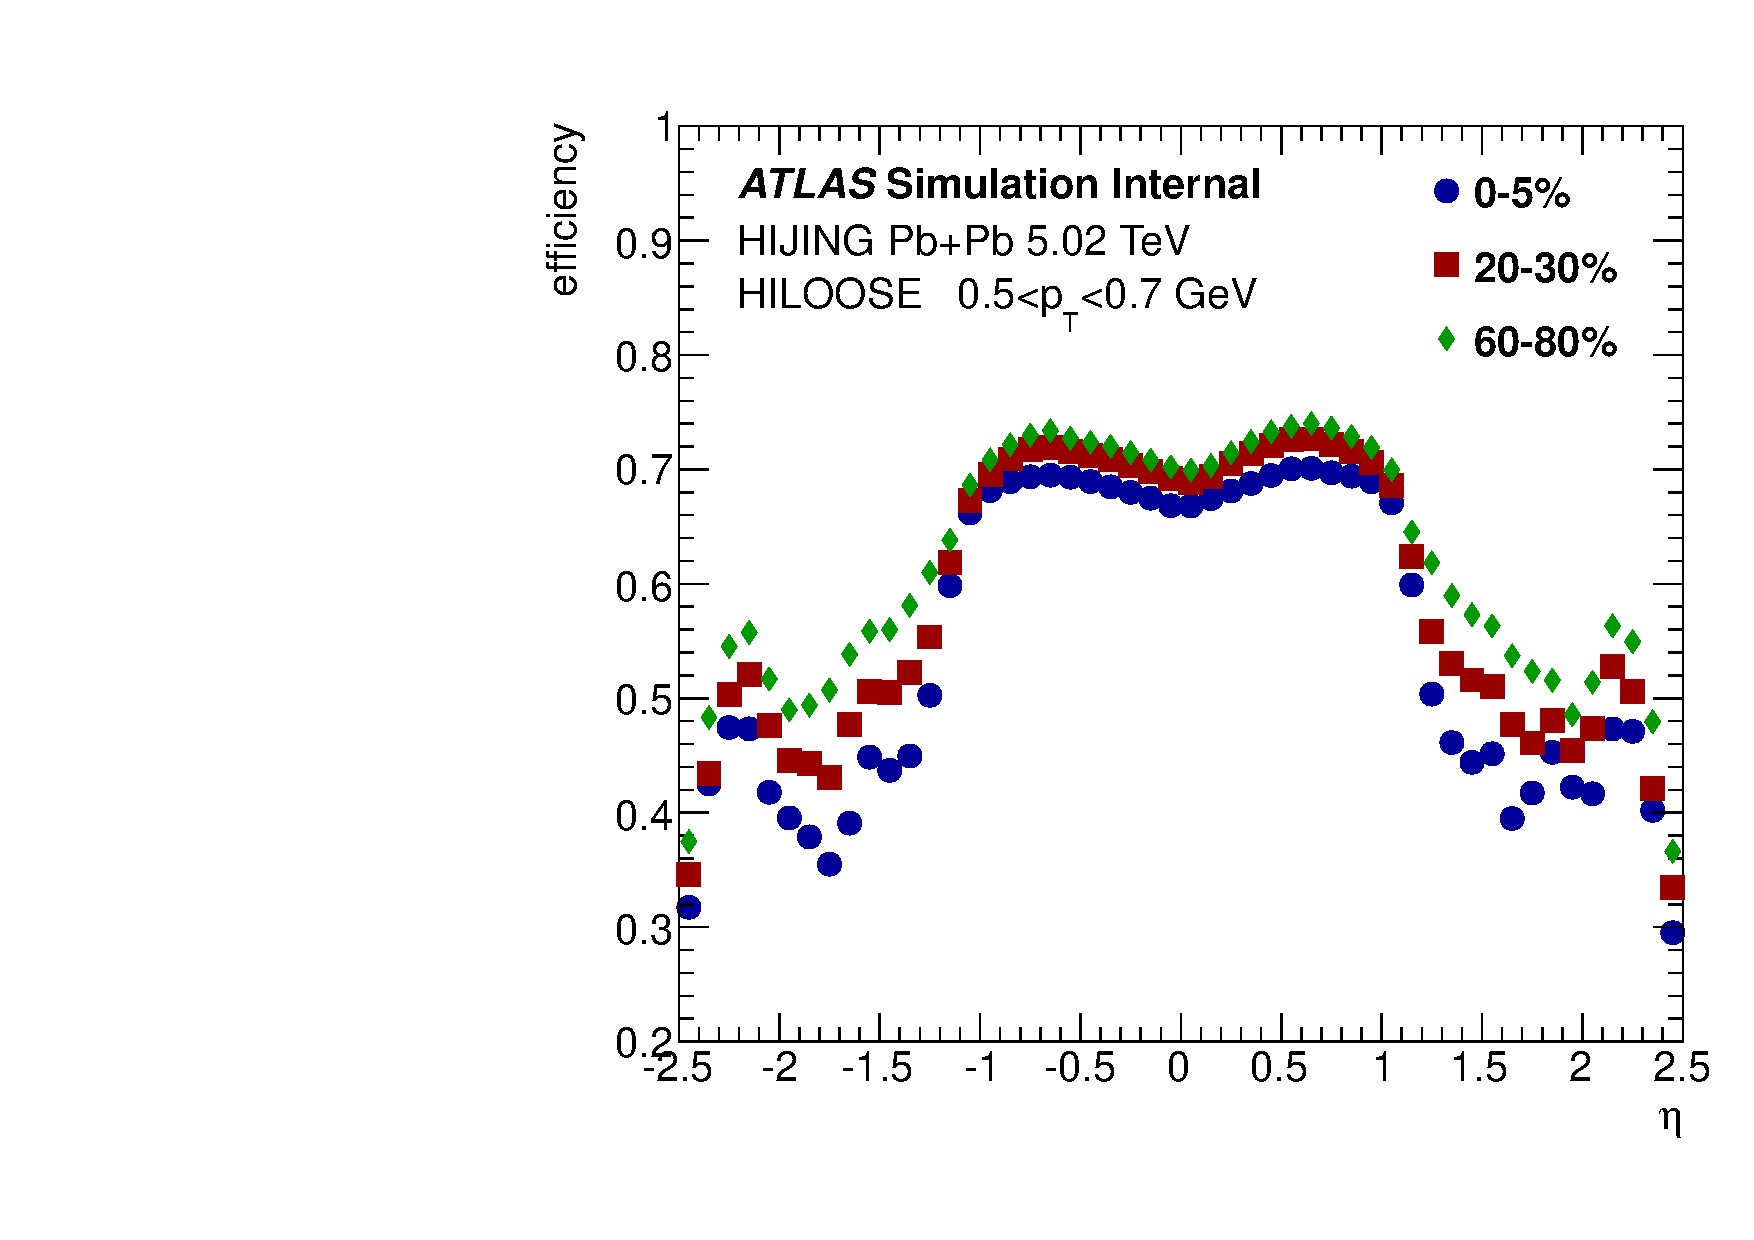
\includegraphics[width=.32\linewidth]{figs/sec_trkSel/PbPb502/PbPb502_LOOSE_eff_Pt0.pdf}
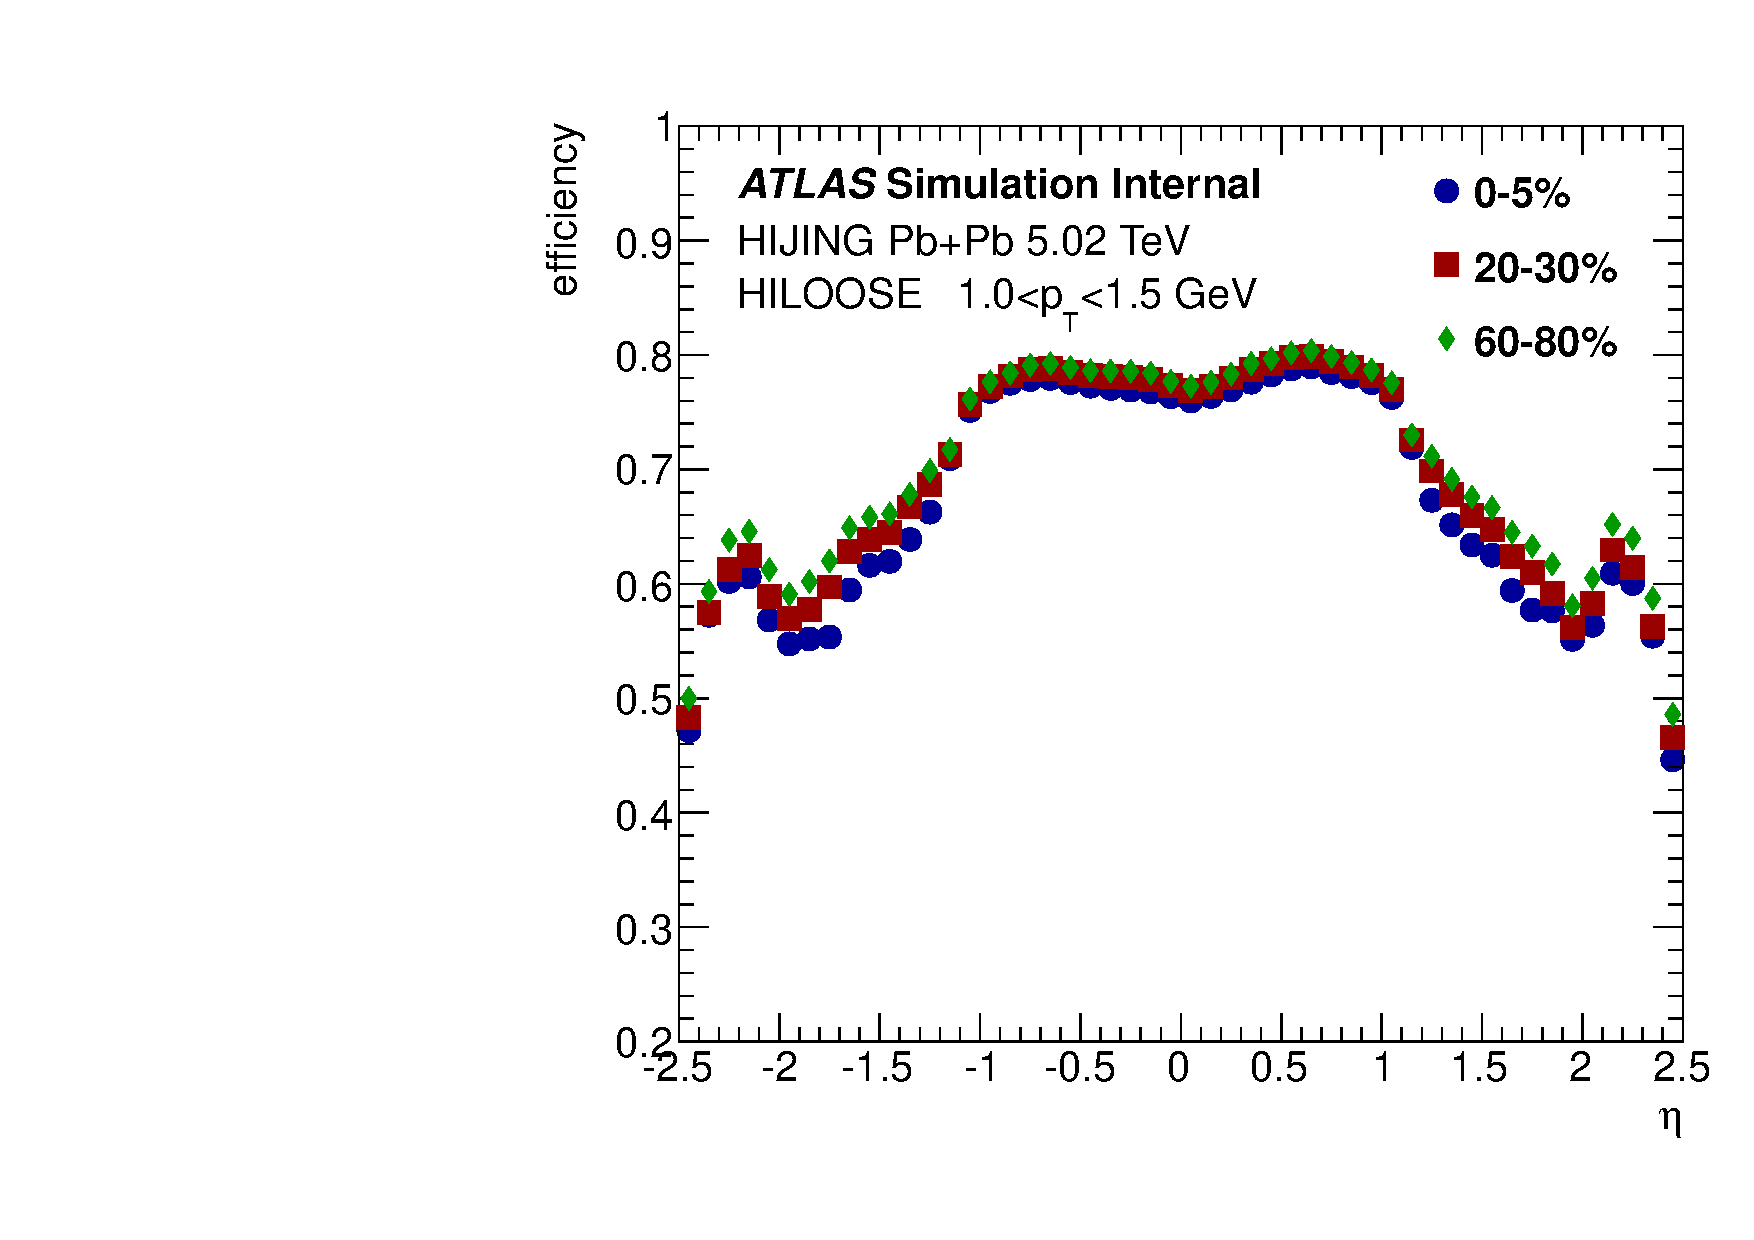
\includegraphics[width=.32\linewidth]{figs/sec_trkSel/PbPb502/PbPb502_LOOSE_eff_Pt2.pdf}
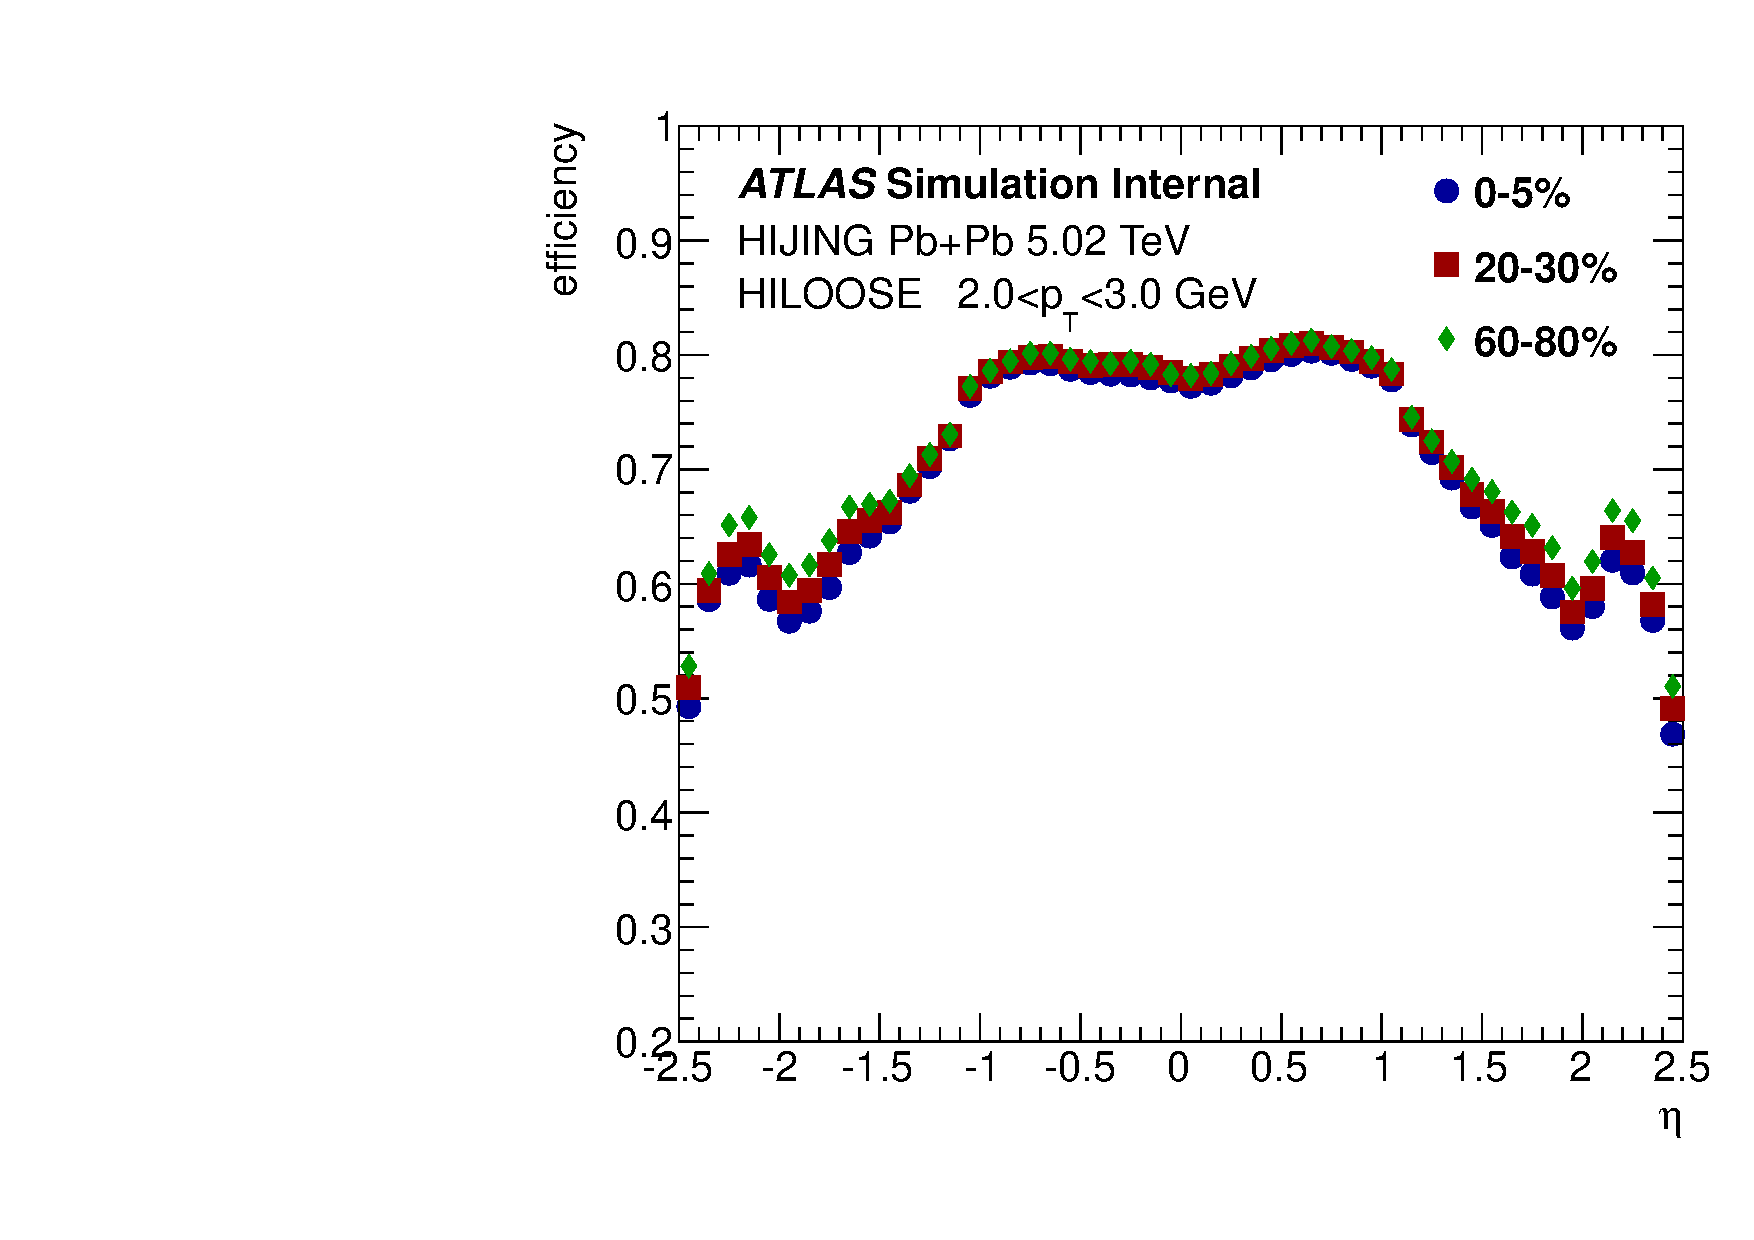
\includegraphics[width=.32\linewidth]{figs/sec_trkSel/PbPb502/PbPb502_LOOSE_eff_Pt4.pdf}
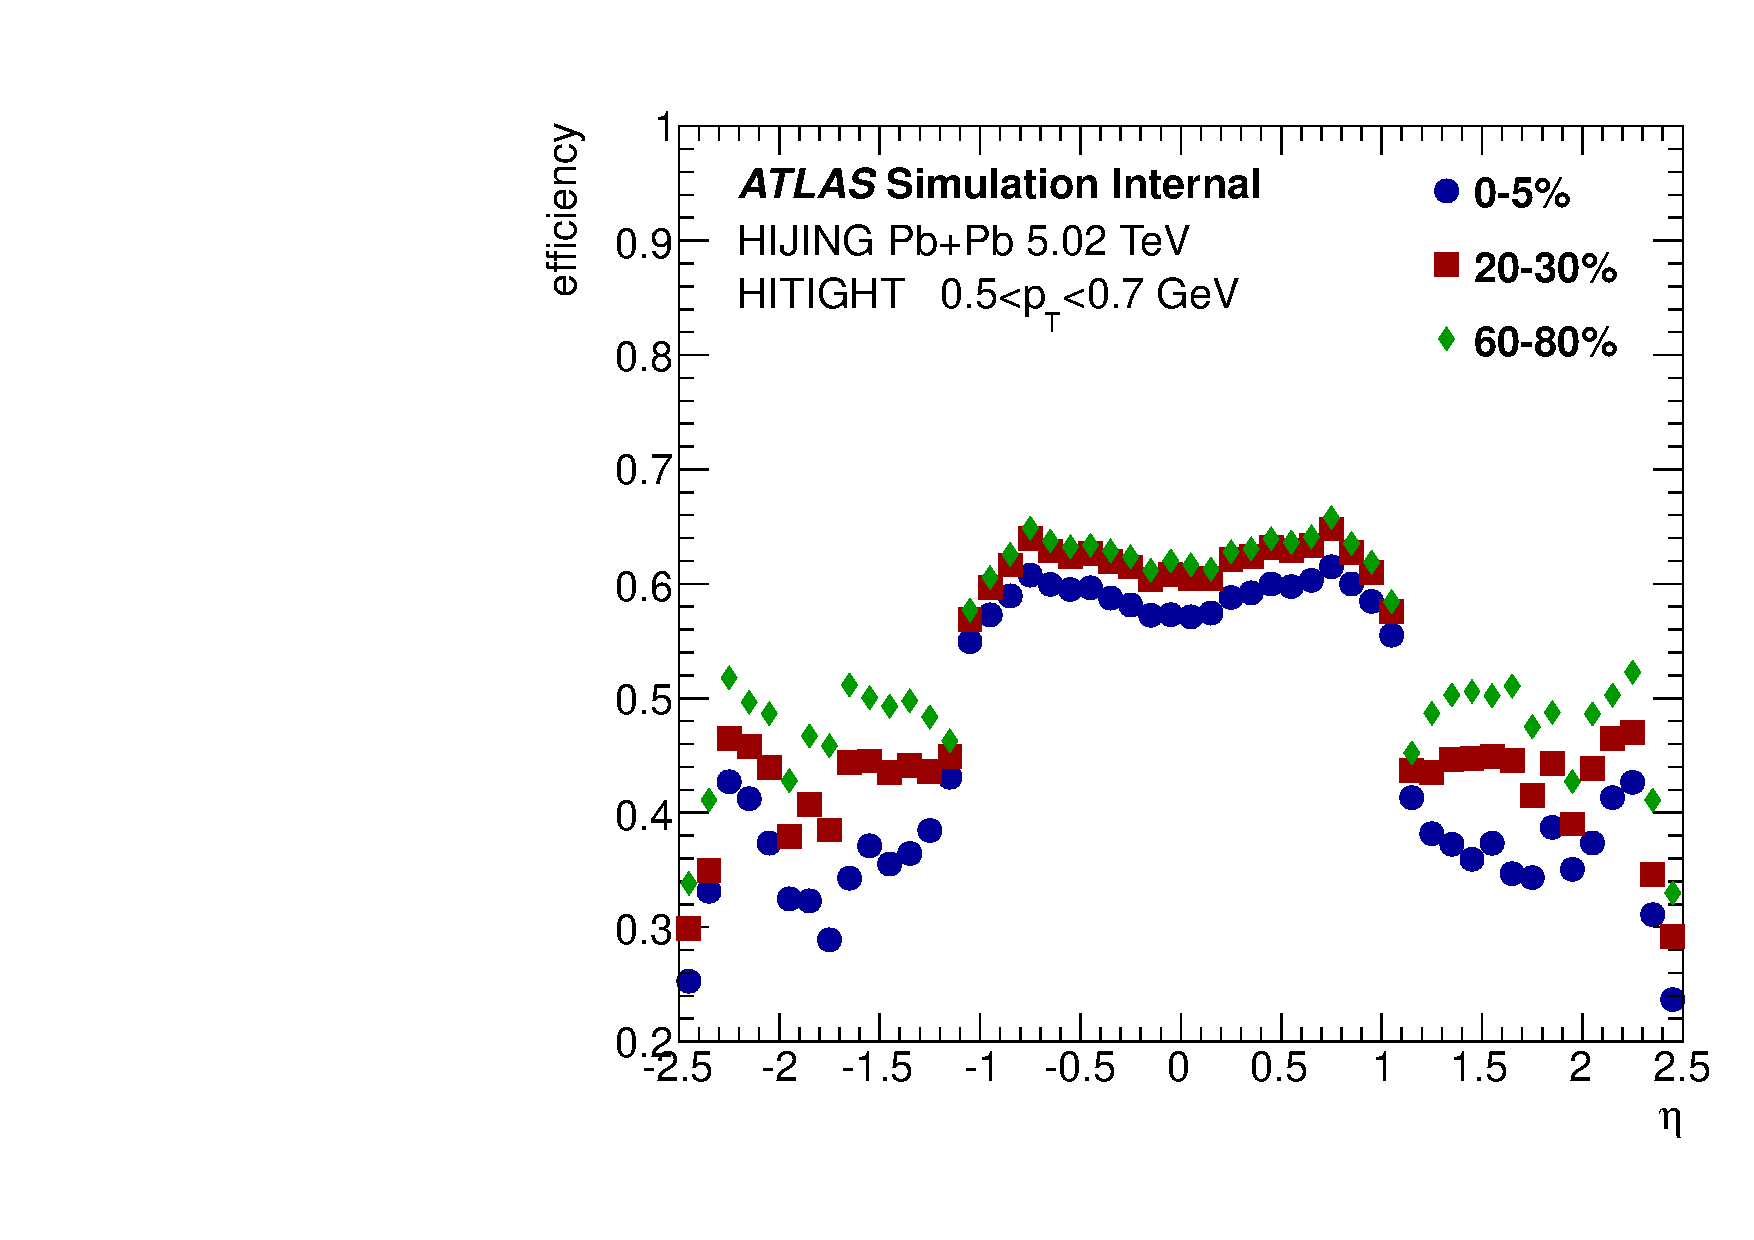
\includegraphics[width=.32\linewidth]{figs/sec_trkSel/PbPb502/PbPb502_TIGHT_eff_Pt0.pdf}
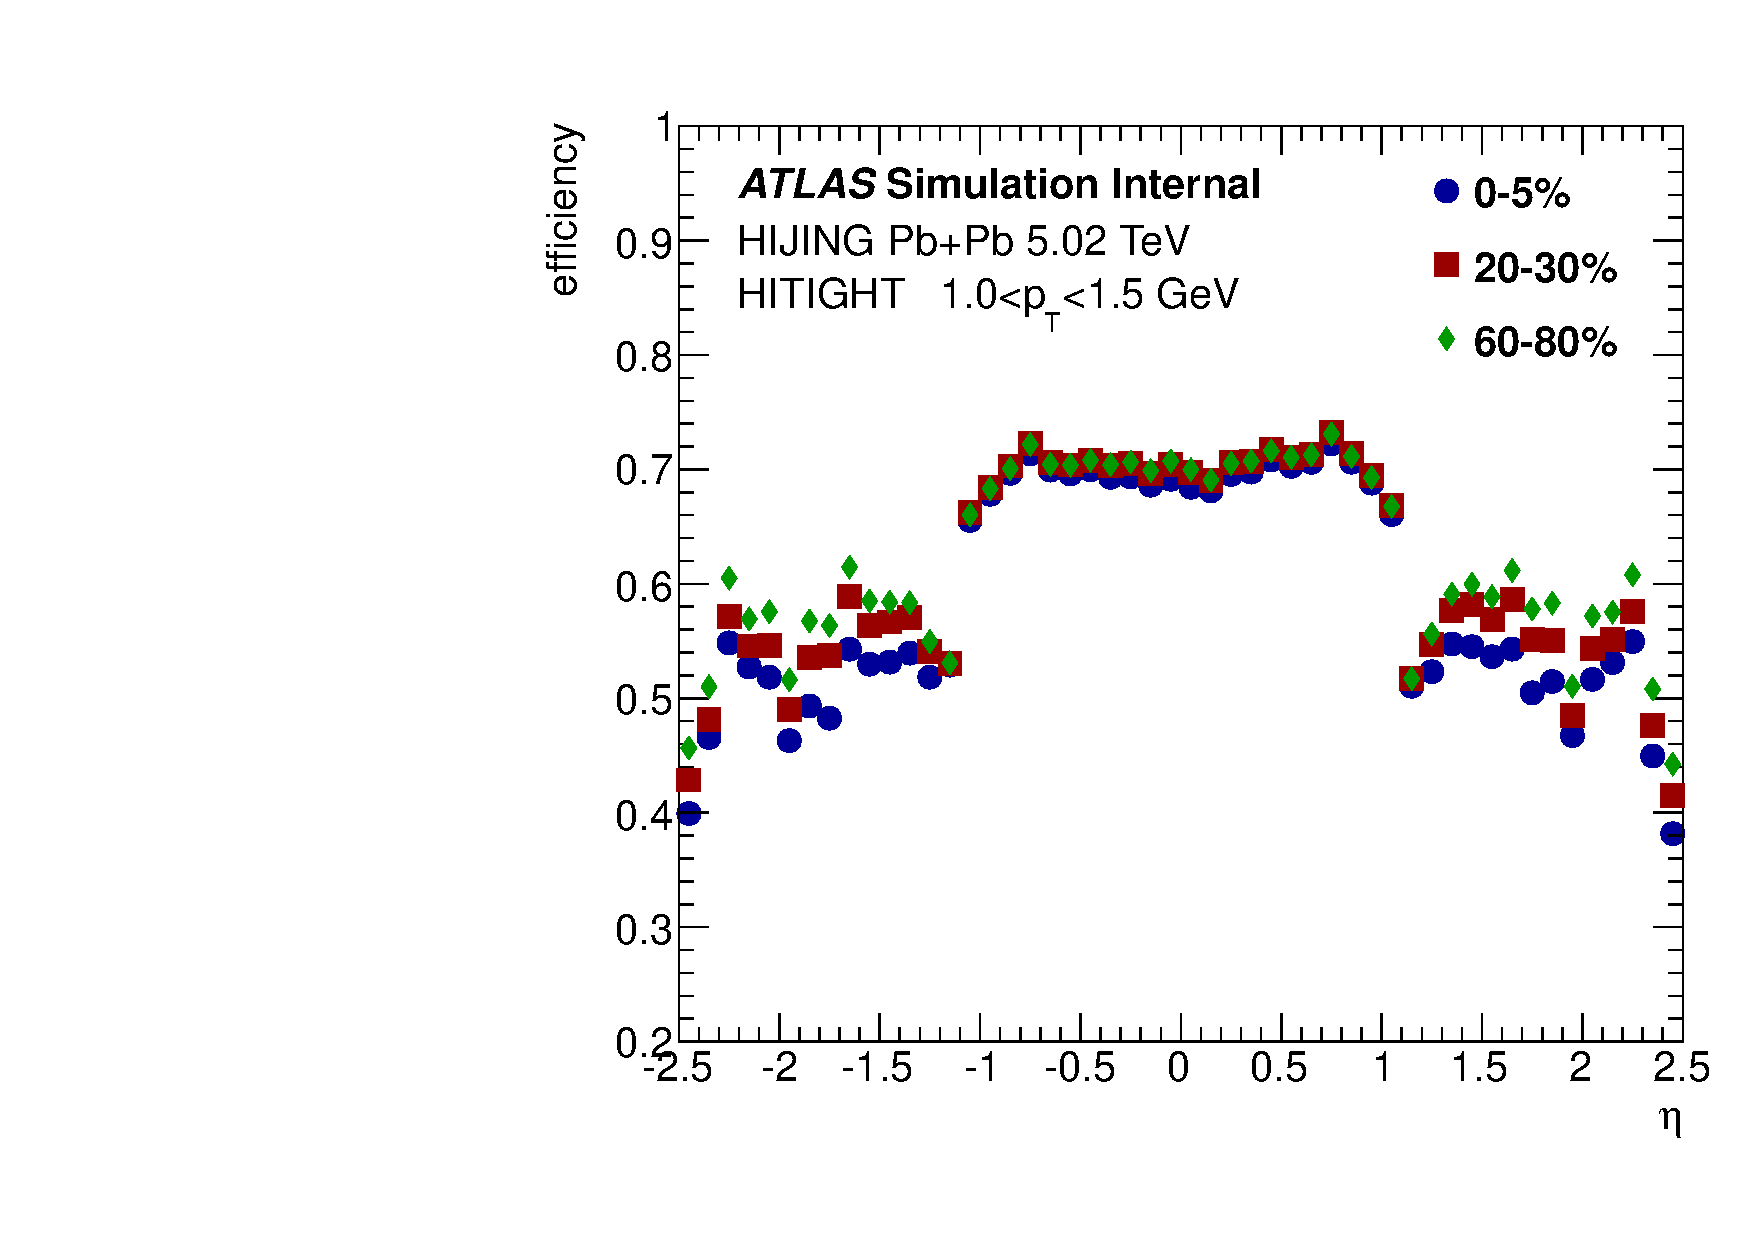
\includegraphics[width=.32\linewidth]{figs/sec_trkSel/PbPb502/PbPb502_TIGHT_eff_Pt2.pdf}
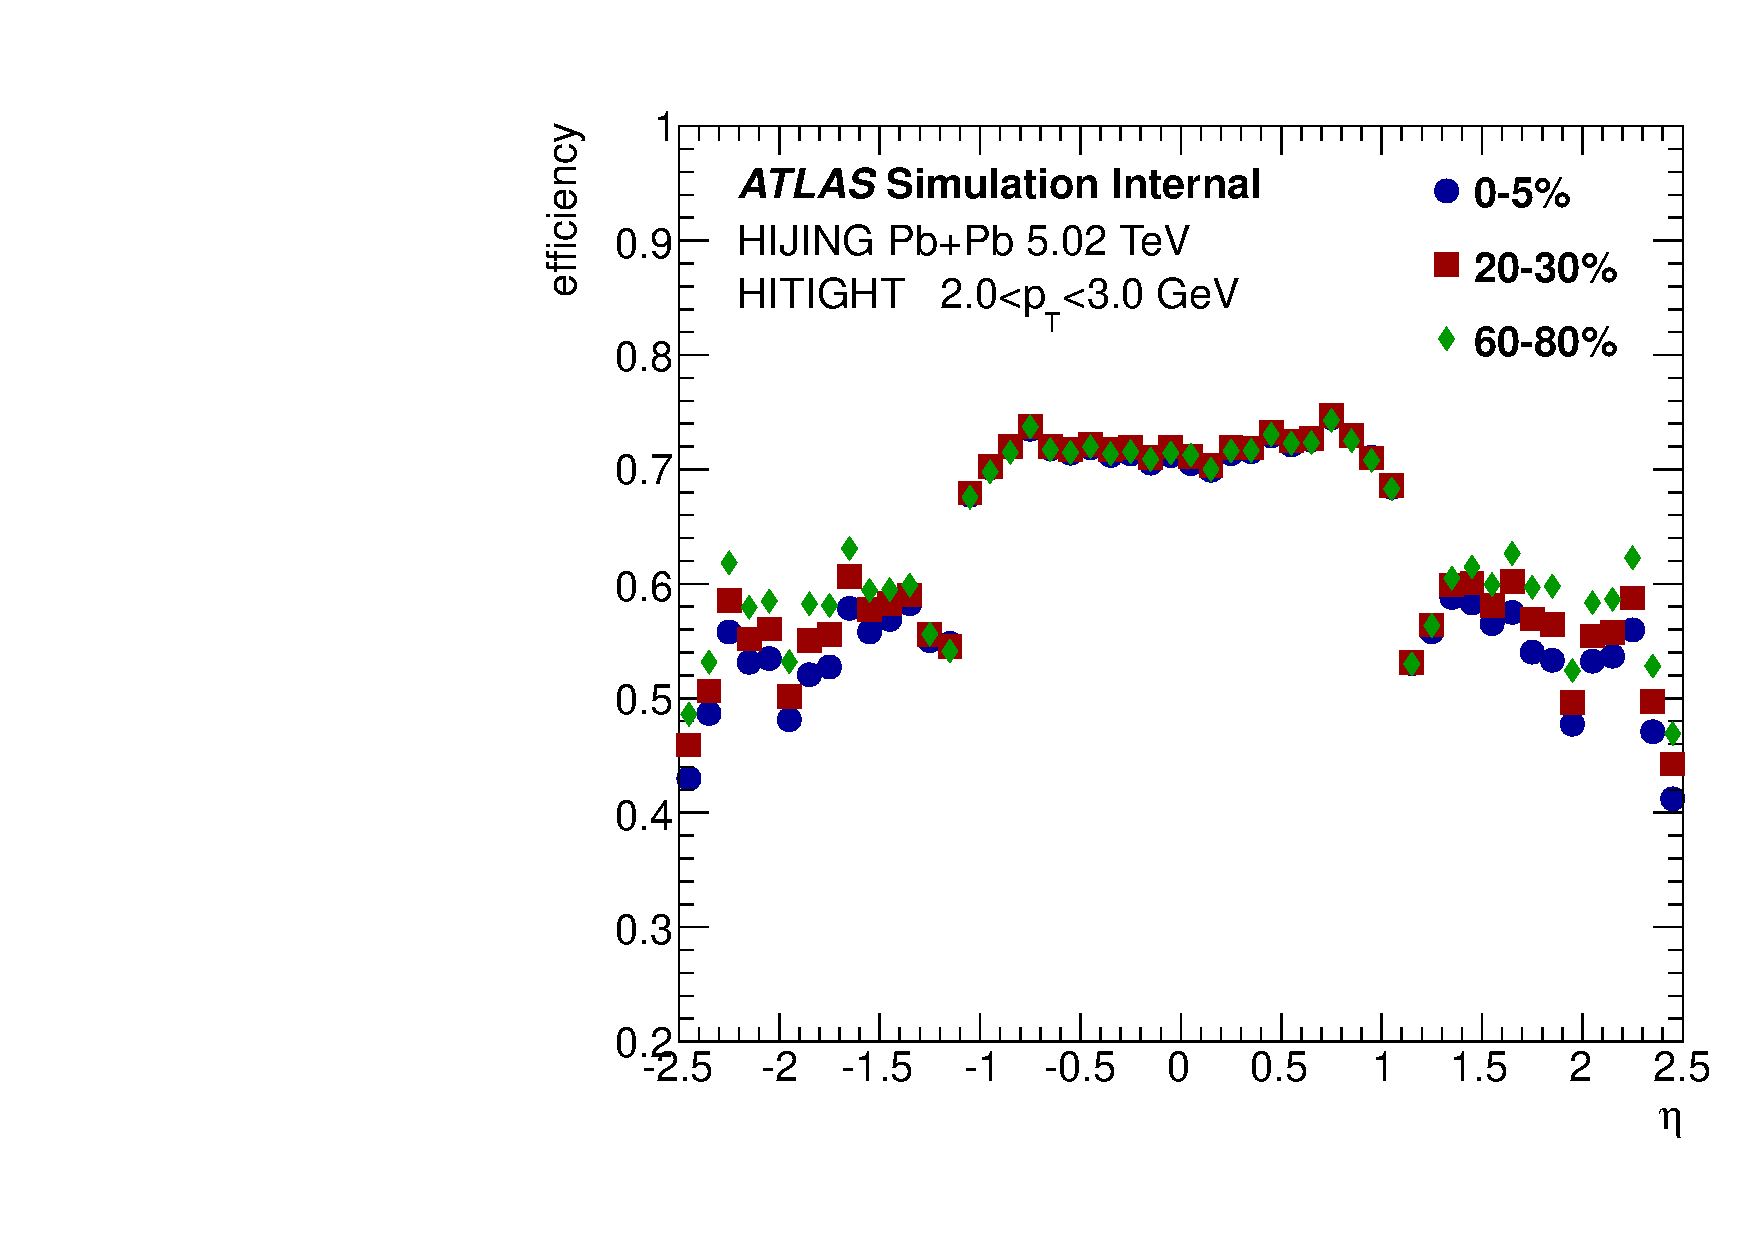
\includegraphics[width=.32\linewidth]{figs/sec_trkSel/PbPb502/PbPb502_TIGHT_eff_Pt4.pdf}
\caption{5.02 TeV Pb+Pb tracking efficiency $\epsilon(\eta)$, for different $p_{\text{T}}$ ranges and centralities. Top row is for loose track quality cut (default) and bottom row is for tight cut.}
\label{fig:PbPb502_trkEff}
\end{figure}



\subsection{Fakes}
Since one of the focuses in this analysis is on ultra-central collisions, fake rate correction $1-f$ were applied to the efficiency $\epsilon$ and each track is weighted by $(1-f)/\ \epsilon$. The fake rates map is also borrowed from Run 2 $v_n$ analysis~\cite{Burka:2151932}, which is evaluated as a function of $p_{\text{T}}, \eta$ and centrality. To estimate the fraction of fake tracks, the track selection follows the loose quality cut. The fake rate $f(\eta)$ are shown in Fig.~\ref{fig:PbPb502_trkFak}, for different $p_{\text{T}}$ ranges and centrality. $f(\eta)$ is lowest in mid-rapidity $-1<\eta<1$, and increases by more than 2 times in forward-rapidity. As collision moves to peripheral, the fake rate significantly decreases. The fake rate decreases significantly towards higher $p_{\text{T}}$. Fake rate from $\verb|HILOOSE|$ is higher than $\verb|HITIGHT|$ as expected.
\begin{figure} [H]
\centering
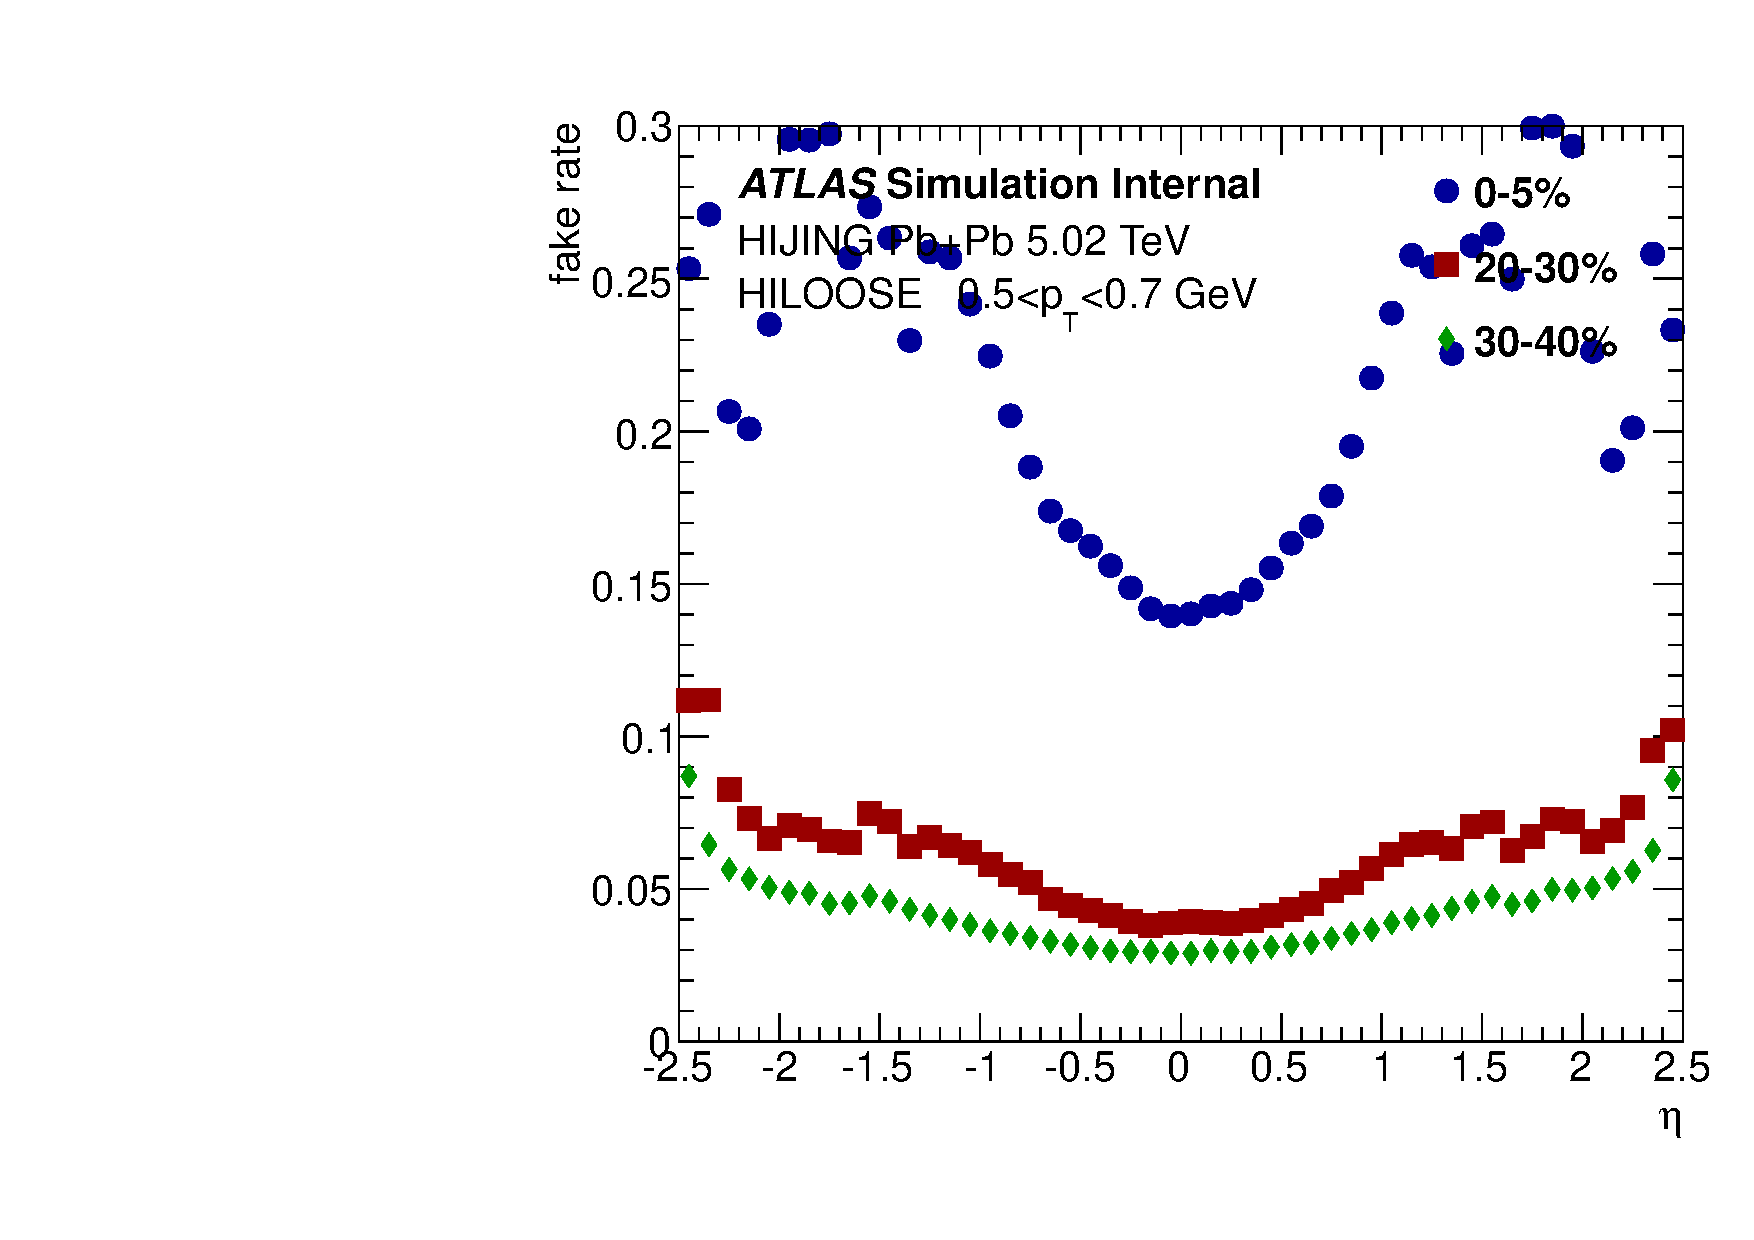
\includegraphics[width=.32\linewidth]{figs/sec_trkSel/PbPb502/PbPb502_LOOSE_fak_Pt0.pdf}
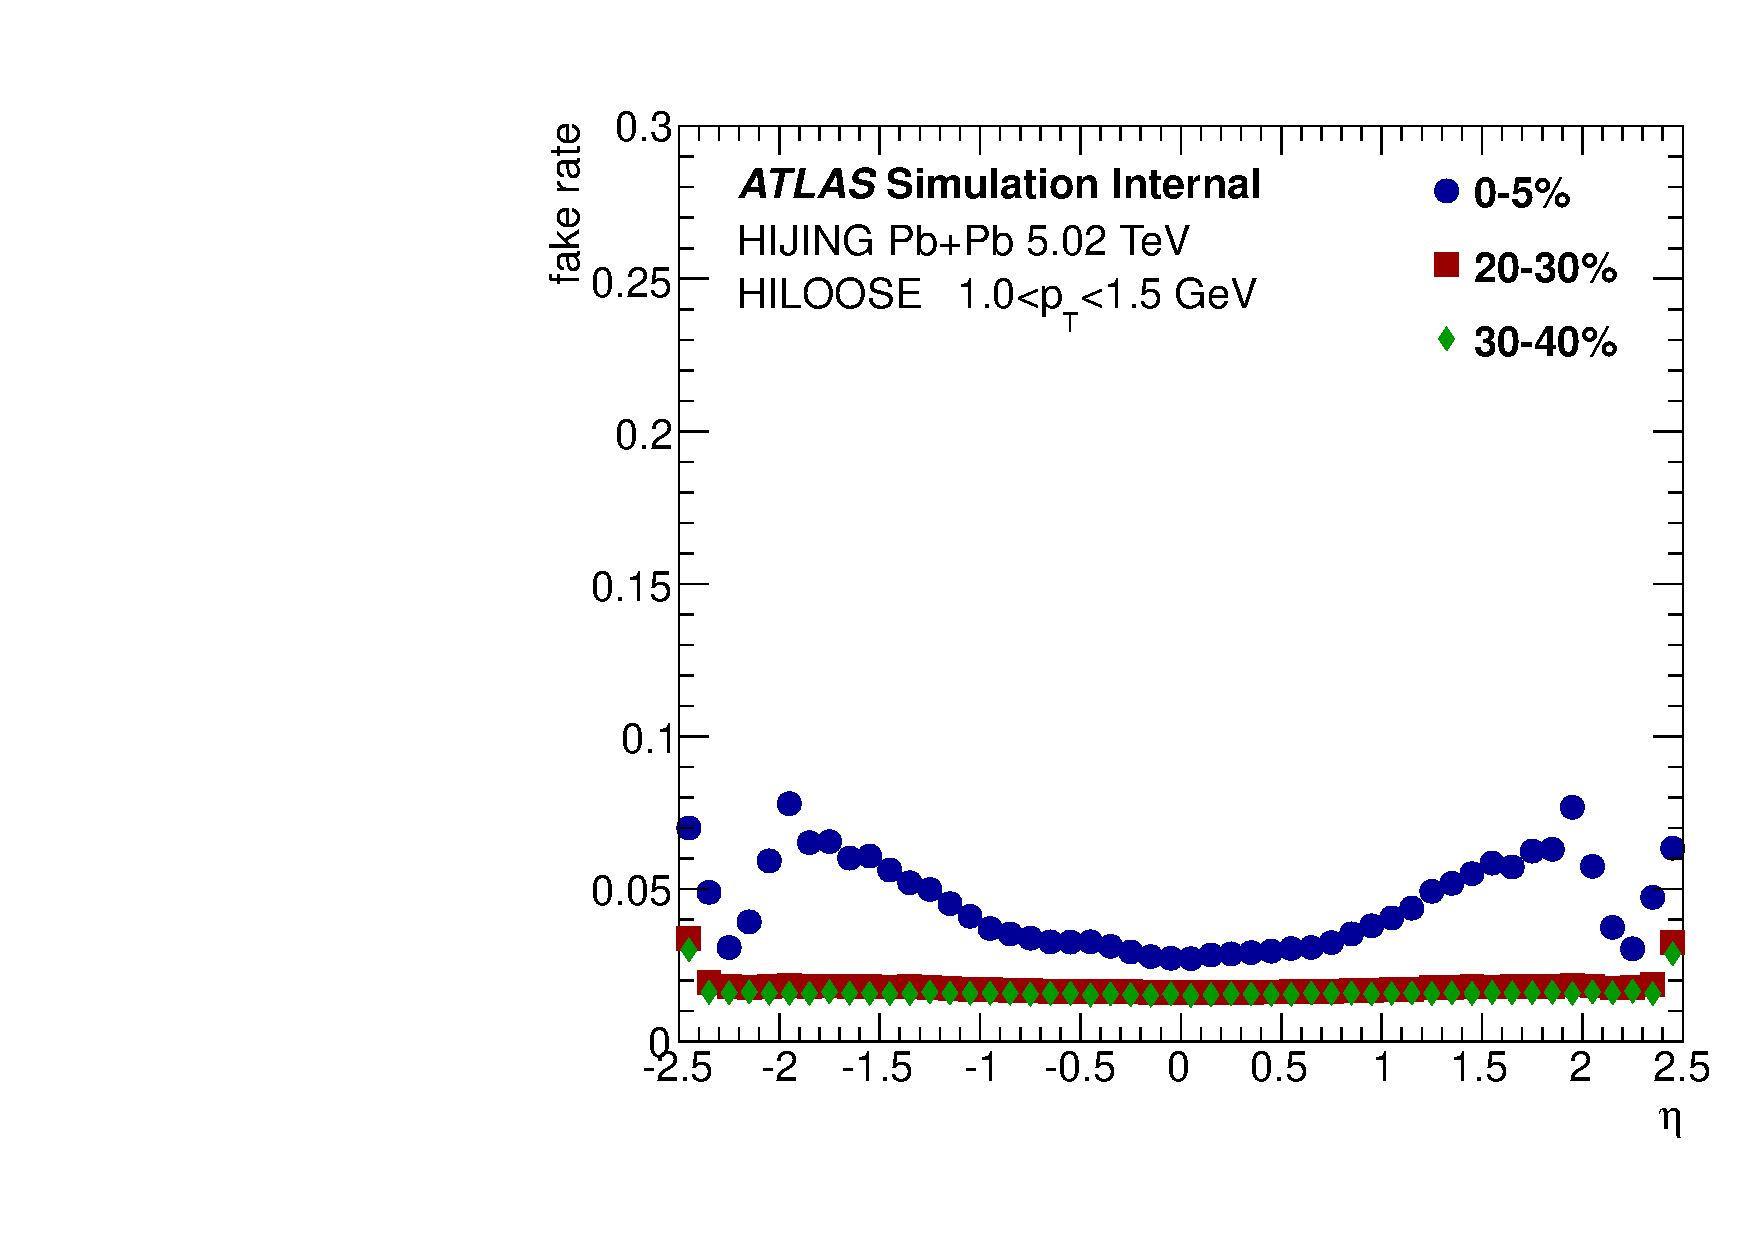
\includegraphics[width=.32\linewidth]{figs/sec_trkSel/PbPb502/PbPb502_LOOSE_fak_Pt2.pdf}
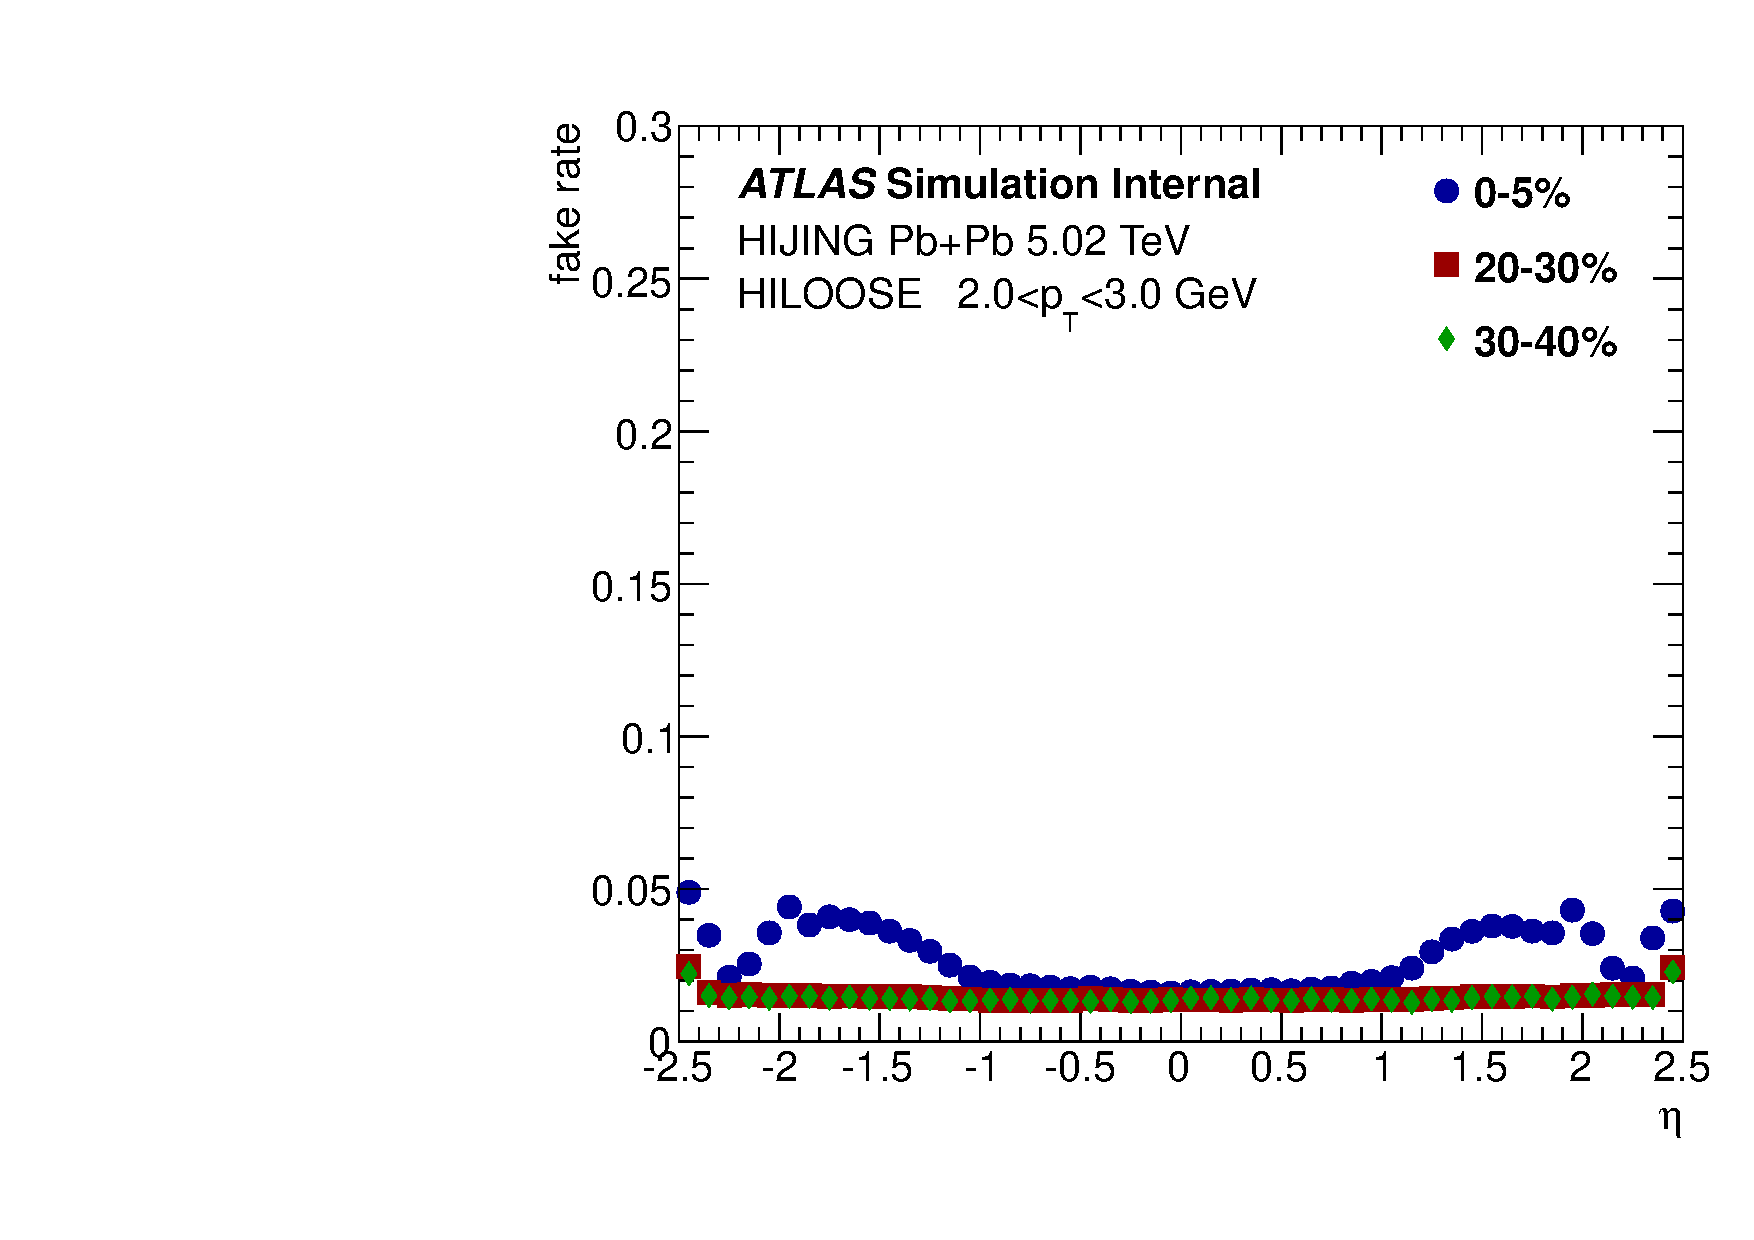
\includegraphics[width=.32\linewidth]{figs/sec_trkSel/PbPb502/PbPb502_LOOSE_fak_Pt4.pdf}
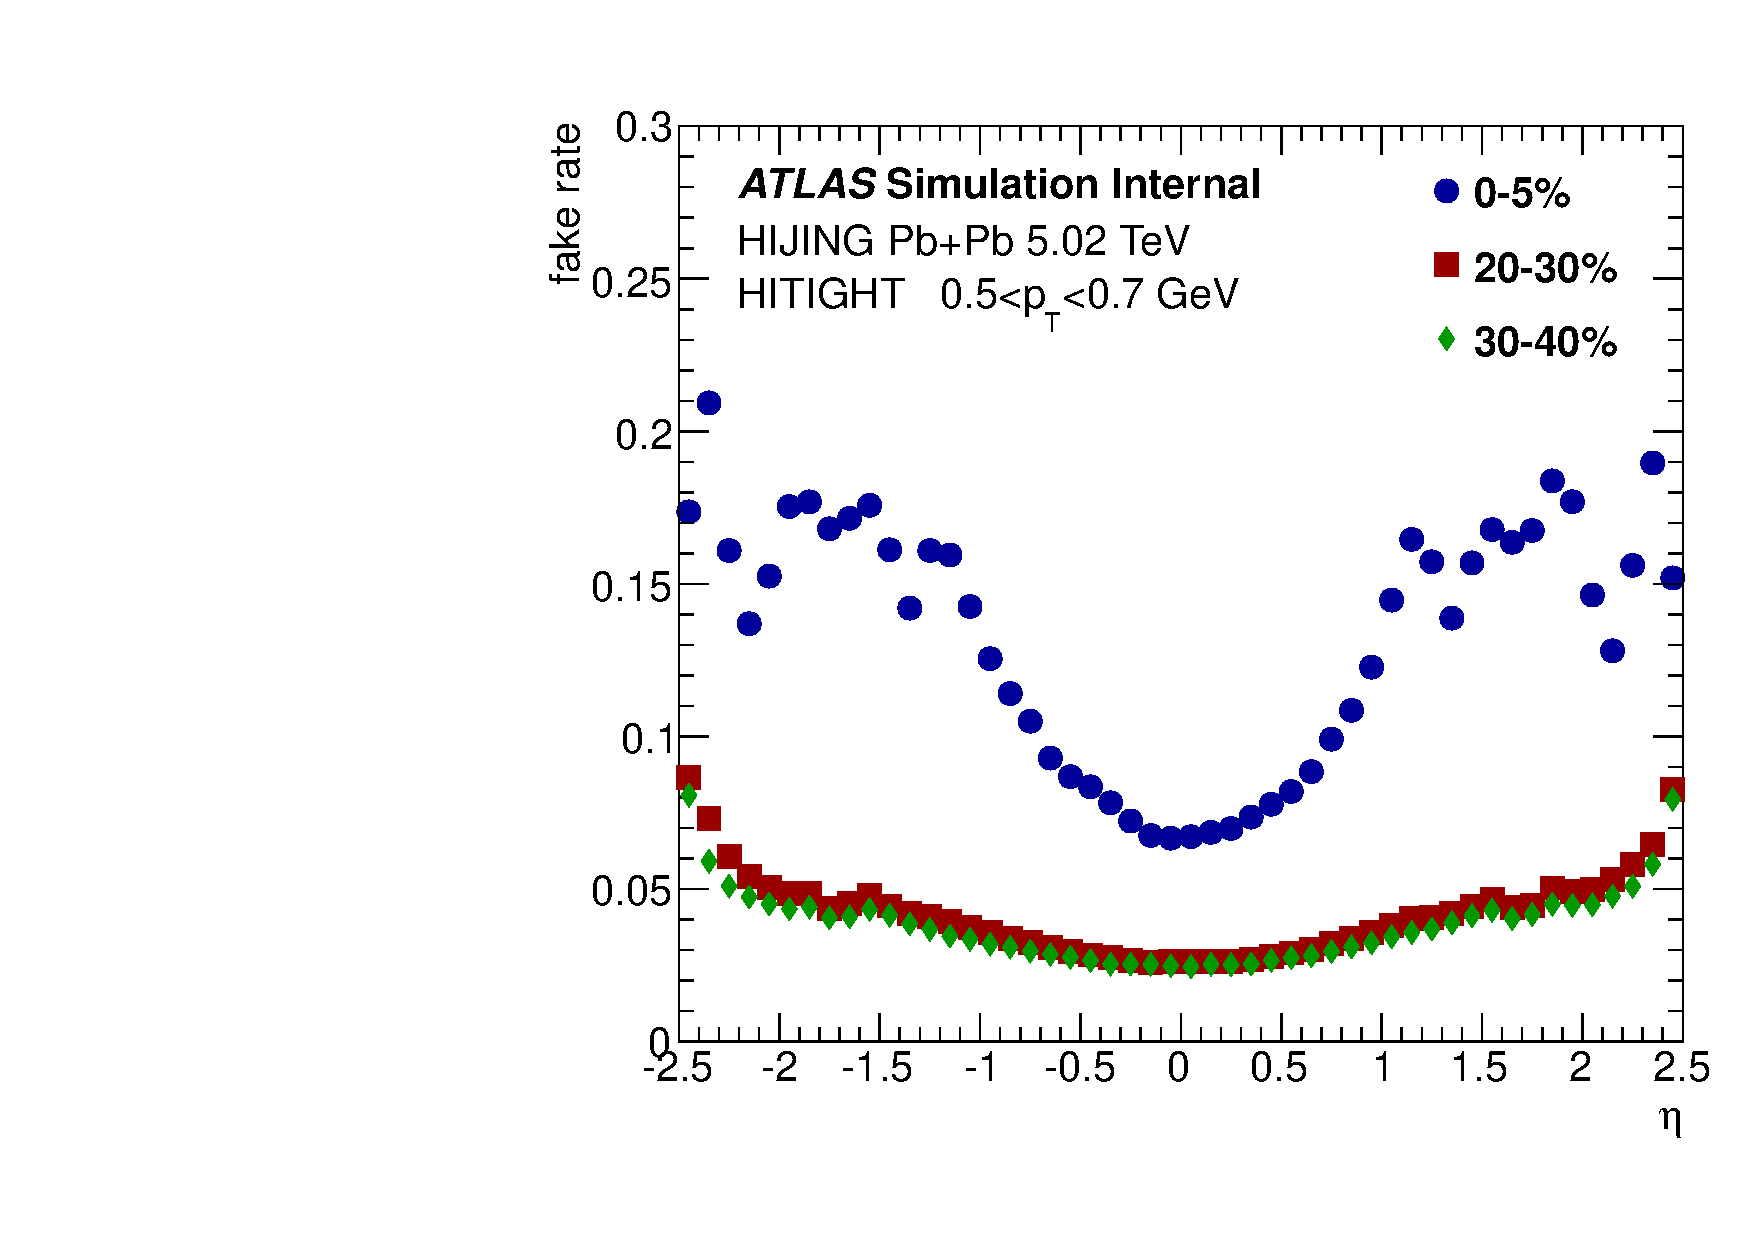
\includegraphics[width=.32\linewidth]{figs/sec_trkSel/PbPb502/PbPb502_TIGHT_fak_Pt0.pdf}
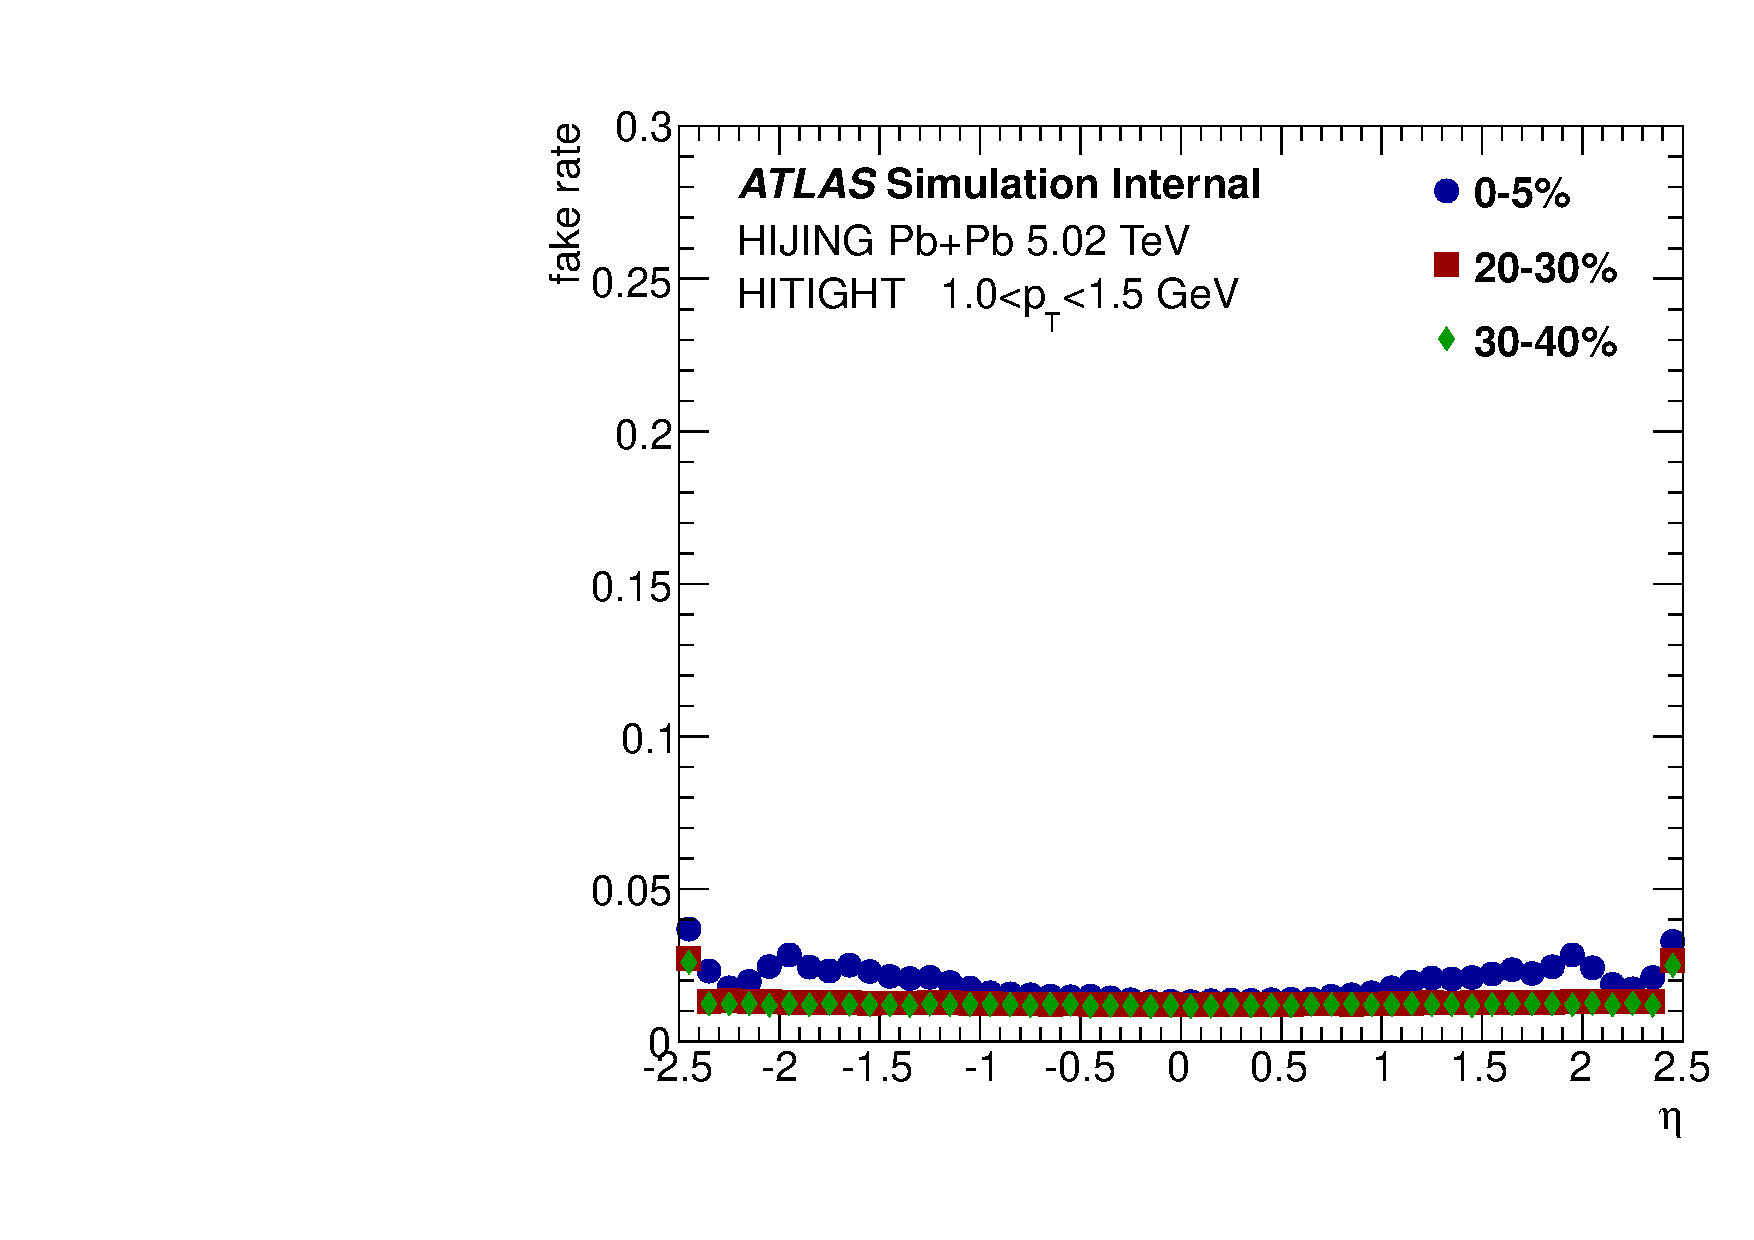
\includegraphics[width=.32\linewidth]{figs/sec_trkSel/PbPb502/PbPb502_TIGHT_fak_Pt2.pdf}
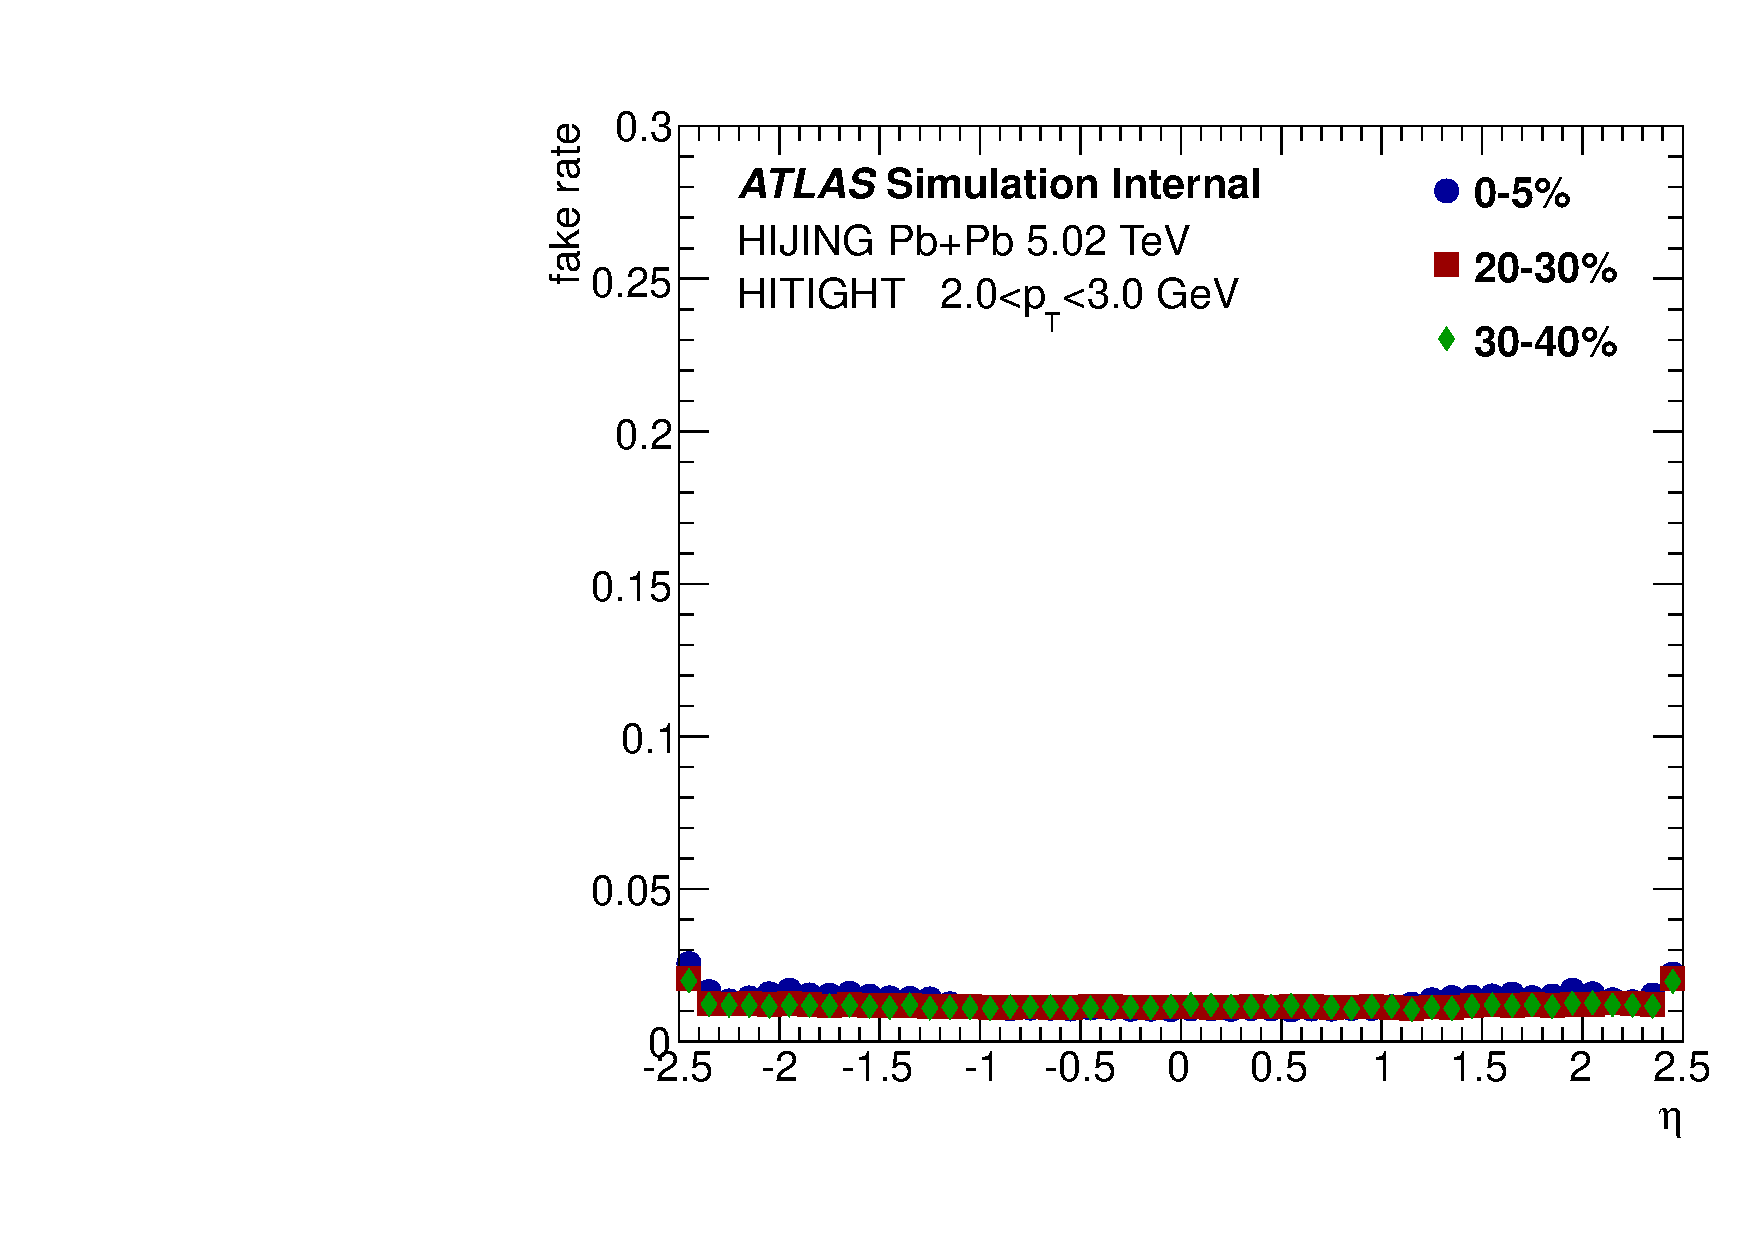
\includegraphics[width=.32\linewidth]{figs/sec_trkSel/PbPb502/PbPb502_TIGHT_fak_Pt4.pdf}
\caption{5.02 TeV Pb+Pb tracking fake rates $f(\eta)$, for different $p_{\text{T}}$ ranges and centralities. Top row is for loose track quality cut (default) and bottom row is for tight cut.}
\label{fig:PbPb502_trkFak}
\end{figure}




\clearpage

\section{Methodology}
\label{sec:method}
\subsection{Outline}
The details of cumulant analysis are carried out in the following procedures:
\begin{itemize}
\item Calculation of 2-, 4- and 6-particle correlation $corr_n\{2k\}$:
\begin{itemize}
\item Standard cumulant method;
\item 3-subevent cumulant method;
\end{itemize}
\item Calculation of 2-, 4- and 6-particle cumulant $c_n\{2k\}$:
\begin{itemize}
\item Standard cumulant method;
\item 3-subevent cumulant method;
\end{itemize}
\item Calculation of 2-, 4- and 6-particle flow signal $v_n\{2k\}$;
\item Calculation of normalized cumulant $nc_n\{2k\}$;
\item Universality check of flow fluctuation models;
\item Calculation of symmetric cumulant $sc_{n,m}\{4\}$ and $nsc_{n,m}\{4\}$;
\begin{itemize}
\item Standard symmetric cumulant method;
\item 3-subevent symmetric cumulant method;
\end{itemize}
\item Calculation of asymmetric cumulant $ac_{n,n+m}\{3\}$ and $nac_{n,n+m}\{3\}$;
\begin{itemize}
\item Standard asymmetric cumulant method;
\item 3-subevent asymmetric cumulant method;
\end{itemize}
\end{itemize}



\subsection{Calculation of 2-, 4- and 6-particle correlation $corr_n\{2k\}$}
2-, 4- and 6-particle correlations are defined as:
\begin{equation}
\begin{split}
corr_n\{2\}&\equiv \lr{e^{\text{i}n(\phi_i-\phi_j)}} \\
corr_n\{4\}&\equiv \lr{e^{\text{i}n(\phi_i+\phi_j-\phi_k-\phi_l)}} \\
corr_n\{6\}&\equiv \lr{e^{\text{i}n(\phi_i+\phi_j+\phi_k-\phi_l-\phi_m-\phi_n)}}
\end{split}
\end{equation}
where notation $corr_n\{2k\}$ is used for the $2k$-particle correlations and $n$ denotes harmonic $n$ in the Fourier coefficients $v_n$. $i, j, k, l, m, n$ denotes unique particles in certain phase space $(p_\text{T},\eta)$, which will be quantified in the analysis section. $\lr{...}$ is the weighted average calculated for each event
\begin{equation}
\begin{split}
\lr{e^{\text{i}n(\phi_i-\phi_j)}}&\equiv \frac{\sum^{'}{w_i w_j e^{\text{i}n(\phi_i-\phi_j)}}}{\sum^{'}{w_i w_j}} \\
\lr{e^{\text{i}n(\phi_i+\phi_j-\phi_k-\phi_l)}}&\equiv \frac{\sum^{'}{w_i w_j w_k w_l e^{\text{i}n(\phi_i+\phi_j-\phi_k-\phi_l)}}}{\sum^{'}{w_i w_j w_k w_l}} \\
\lr{e^{\text{i}n(\phi_i+\phi_j+\phi_k-\phi_l-\phi_m-\phi_n)}}&\equiv \frac{\sum^{'}{w_i w_j w_k w_l w_m w_n e^{\text{i}n(\phi_i+\phi_j+\phi_k-\phi_l-\phi_m-\phi_n)}}}{\sum^{'}{w_i w_j w_k w_l w_m w_n}}
\end{split}
\end{equation}
where $\sum^{'}$ means the summation of unique particles: i.e. $i\neq j$, $i\neq j\neq k\neq l$ and $i\neq j\neq k\neq l\neq m\neq n$ respectively. $w$ is the weight applied to each particle, which is a combination of tracking efficiency $\epsilon$, fraction of fake tracks $f$ and trigger re-weighting $w_{trig}$:
\begin{equation}
w\equiv\frac{w_{\phi}(1-f)}{\epsilon}
\end{equation}
where all these weights will be discussed in details in the cumulant analysis section ~\ref{sec:ana}.

The most straightforward way to calculate $2k$-particle correlation $corr_n\{2k\}$ is called nested loop method: counting all the possible unique combinations within $2k$ nested loops of tracks. Since nested loop method has a complexity of $\mathcal{O}(M^{2k})$, where $M$ is the multiplicity in each event, it requires a lot of CPU hours to compute the 6-particle correlation, especially in Pb+Pb collision. An equivalent way is named as $Q$-cumulant (or direct-cumulant) method, which calculates $corr_n\{2k\}$ in a single loop, thus greatly reduces the complexity to $\mathcal{O}(M)$. The $Q$-cumulant method carefully removes all the correlations between same particles ("duplicates") by using simple diagrams. In this note, we will only list all the formula using $Q$-cumulant, without going into details about the derivation, and we have confirmed that both nested loop and $Q$-cumulant methods give identical results, which validates all the formulas we have used for the Q-cumulant method.


\subsubsection{Standard $Q$-cumulant method}
The event-by-event $\pmb{Q}_{n,k}$ vector in standard cumulant method is defined as:
\begin{equation}
\pmb{Q}_{n,k}\equiv\sum{w_i^k e^{\text{i}n\phi_i}}
\end{equation}
where $w_i$ is the particle weight introduced earlier and the power $k$ is for the purpose of removing duplicates. $n$ denotes the harmonic $n$ from the Fourier coefficients $v_n$.

In order to simply the expression, $S_{p,k}$ is introduced as:
\begin{equation}
S_{p,k}\equiv(\sum{w_i^k})^{p}
\end{equation}
where $k$ in $S_{p,k}$ is the same one with $k$ in $\pmb{Q}_{n,k}$. Note that unlike $\pmb{Q}_{n,k}$, $S_{p,k}$ is not related to the azimuthal angle $\phi$ of each particle.

The $\pmb{Q}_{n,k}$ and $S_{p,k}$ are defined in this way so that $2k$-particle correlation $corr_n\{2k\}$ can be expressed as a function of $\pmb{Q}_{n,k}$ and $S_{p,k}$:
\begin{equation}
corr_n\{2k\}=f(\pmb{Q}_{n,k},S_{p,k})
\end{equation}

The event-by-event 2-, 4- and 6-particle correlations in the standard $Q$-cumulant method can then be written as~\cite{Bilandzic:2010jr}:
\begin{equation}
\begin{split}
corr_n\{2\}&=\frac{|Q_{n,1}|^2-S_{1,2}}{S_{2,1}-S_{1,2}} \\
corr_n\{4\}&=\frac{|Q_{n,1}|^4+|Q_{2n,2}|^2-2\mathcal{R}\textit{e}(\pmb{Q}_{2n,2}\pmb{Q}_{n,1}^*\pmb{Q}_{n,1}^*)+8\mathcal{R}\textit{e}(\pmb{Q}_{n,3}\pmb{Q}_{n,1}^*)-4S_{1,2}|Q_{n,1}|^2+2S_{2,2}-6S_{1,4}}{S_{4,1}+8S_{1,3}S_{1,1}-6S_{1,2}S_{2,1}+3S_{2,2}-6S_{1,4}} \\
corr_n\{6\}&=(|Q_{n,1}|^6-6|Q_{n,1}|^2\mathcal{R}\textit{e}(\pmb{Q}_{2n,2}\pmb{Q}_{n,1}^*\pmb{Q}_{n,1}^*)+9|Q_{2n,2}|^2|Q_{n,1}|^2+4\mathcal{R}\textit{e}(\pmb{Q}_{3n,3}\pmb{Q}_{n,1}^*\pmb{Q}_{n,1}^*\pmb{Q}_{n,1}^*) \\
&+18S_{1,2}\mathcal{R}\textit{e}(\pmb{Q}_{2n,2}\pmb{Q}_{n,1}^*\pmb{Q}_{n,1}^*)-36\mathcal{R}\textit{e}(\pmb{Q}_{2n,4}\pmb{Q}_{n,1}^*\pmb{Q}_{n,1}^*)-36\mathcal{R}\textit{e}(\pmb{Q}_{n,3}\pmb{Q}_{n,1}\pmb{Q}_{2n,2}^*)+18S_{2,2}|Q_{n,1}|^2 \\
&-54S_{1,4}|Q_{n,1}|^2-72S_{1,2}\mathcal{R}\textit{e}(\pmb{Q}_{n,3}\pmb{Q}_{n,1}^*)+36|Q_{n,3}|^2+144\mathcal{R}\textit{e}(\pmb{Q}_{n,5}\pmb{Q}_{n,1}^*)-9S_{1,2}|Q_{n,1}|^4 \\
&+36|Q_{n,1}|^2\mathcal{R}\textit{e}(\pmb{Q}_{n,3}\pmb{Q}_{n,1}^*)-9S_{1,2}|Q_{2n,2}|^2+36\mathcal{R}\textit{e}(\pmb{Q}_{2n,4}\pmb{Q}_{2n,2}^*)-12\mathcal{R}\textit{e}(\pmb{Q}_{3n,3}\pmb{Q}_{2n,2}^*\pmb{Q}_{n,1}^*) \\
&+4|Q_{3n,3}|^2+54S_{1,4}S_{1,2}-6S_{3,2}-120S_{1,6})/(S_{6,1}-15S_{1,2}S_{4,1}+40S_{1,3}S_{3,1}+45S_{2,2}S_{2,1} \\
&-90S_{1,4}S_{2,1}-120S_{1,3}S_{1,2}S_{1,1}-15S_{3,2}+144S_{1,5}S_{1,1}+90S_{1,4}S_{1,2}+40S_{2,3}-120S_{1,6})
\end{split}
\end{equation}


\subsubsection{3-subevent $Q$-cumulant method}
Compared with standard method, the format of $corr_n\{2k\}$ are slightly altered in the 3-subevent method:
\begin{equation}
\begin{split}
corr_n^{a|b}\{2\}&\equiv \lr{e^{\text{i}n(\phi_a-\phi_b)}} \\
corr_n^{a,a|b,c}\{4\}&\equiv \lr{e^{\text{i}n(\phi_a+\phi_a^{'}-\phi_b-\phi_c)}}
\end{split}
\end{equation}
where notation $a|b$ and $a,a|b,c$ are added to the superscript of $corr_n\{2k\}$ to distinguish formula from the standard method. Moreover, particles $i,j,k$ and $l$ come from 3 subevents with different $\eta$ ranges:
\begin{itemize}
\item $\phi_a$: $\phi$ angle of particle from subevent a;
\item $\phi_b$: $\phi$ angle of particle from subevent b;
\item $\phi_c$: $\phi$ angle of particle from subevent c;
\item $\phi_a^{'}$: $\phi$ angle of particle from subevent a, but different from $\phi_a$;
\end{itemize}
One of the main reasons to measure cumulant is to suppress non-flow contribution, which originates from resonance decay, HBT, jet correlation and so on. In contrast to flow, non-flow usually has fewer particles associated with. By measuring the multi-particle correlation, those non-flow contributions can be mostly removed. However, for example, in the jet scenario, more than 3 particles can be correlated with each other, which can not be removed using the standard cumulant method. Due to this reason, subevent cumulant method is introduced to suppress the residual non-flow. In 3 subevent method, since the 4 particles are required to come from 3 subevents across the whole $\eta$ range, short-range (in $\eta$) non-flow correlations are greatly suppressed. Furthermore, 3-subevent is also robust at reducing long-range non-flow correlations, i.e. back-to-back di-jet correlation. The two correlated jets can only fall into two out of the three subevents, thus there will always be at least one particle in $corr_n\{4\}$ that is not associated with the di-jet. After averaging all the combinations, the di-jet correlation is significantly suppressed. The residual di-jet contribution can be easily evaluated by introducing small $\eta$ gaps between 3 subevents.

The subevent method has been extensively studied and validated in Monte-Carlo models as well as $pp$ data, where the non-flow contribution is much larger than Pb+Pb. The whole purpose of showing subevent results is to confirm that the non-flow is negligible in Pb+Pb: the final results will be presented using standard cumulant method after showing it gives same results as subevent method, since one advantage of standard method is that it has smaller statistical uncertainties. Due to the same reason, 6-particle cumulant is only calculated using standard method, as the fraction of non-flow that containing 6 or more particles is significantly lower.

Due to symmetry, there are other five ways to construct $corr_n\{4\}$ in 3-subevent:
\begin{equation}
\begin{split}
corr_n^{b,b|c,a}\{4\}&\equiv \lr{e^{\text{i}n(\phi_b+\phi_b^{'}-\phi_c-\phi_a)}} \\
corr_n^{c,c|a,b}\{4\}&\equiv \lr{e^{\text{i}n(\phi_c+\phi_c^{'}-\phi_a-\phi_b)}} \\
corr_n^{a,b|a,c}\{4\}&\equiv \lr{e^{\text{i}n(\phi_a+\phi_b-\phi_a^{'}-\phi_c)}} \\
corr_n^{b,c|b,a}\{4\}&\equiv \lr{e^{\text{i}n(\phi_b+\phi_c-\phi_b^{'}-\phi_a)}} \\
corr_n^{c,a|c,b}\{4\}&\equiv \lr{e^{\text{i}n(\phi_c+\phi_a-\phi_c^{'}-\phi_b)}}
\end{split}
\end{equation}
where the first two cases are simply permutations on the default configuration of four particles: 2 particles can come from either subevent a, b or c; These two cases are independent from the default and together all three cases will be included in the 3-subevent cumulant calculation of this analysis. We will briefly discuss how to merge the $corr_n\{4\}$ from these three cases later. While for the last three cases, since terms like $\phi_a-\phi_a^{'}$ calculates the correlation within one subevent, which contains much larger fraction of short-range non-flow contribution. So in this analysis, we will not include the last three cases.

Compared with standard cumulant method, since the number of duplicates in summation $\sum$ are significantly less, the formula of $corr_n\{2k\}$ for 3-subevent is much simpler:
\begin{equation}
\begin{split}
corr_n^{a|b}\{2\}&=\frac{\mathcal{R}\textit{e}(\pmb{Q}_{n,1}^{a}\pmb{Q}_{n,1}^{b*})}{S_{1,1}^a S_{1,1}^b} \\
corr_n^{a,a|b,c}\{4\}&=\frac{\mathcal{R}\textit{e}(\pmb{Q}_{n,1}^a \pmb{Q}_{n,1}^{b*} \pmb{Q}_{n,1}^a \pmb{Q}_{n,1}^{c*})-\mathcal{R}\textit{e}(\pmb{Q}_{2n,2}^a \pmb{Q}_{n,1}^{b*} \pmb{Q}_{n,1}^{c*})}{(S_{2,1}^a-S_{1,2}^a)S_{1,1}^b S_{1,1}^c}
\end{split}
\end{equation}
The other similar configurations $corr_n^{b|c}\{2\}$, $corr_n^{c|a}\{2\}$, $corr_n^{b,b|c,a}\{4\}$ and $corr_n^{c,c|a,b}\{4\}$ can be easily written by permutations of the indices $a$, $b$ and $c$.


\subsection{Calculation of 2-, 4- and 6-particle cumulant $c_n\{2k\}$}
In the last section, event-by-event $2k$-particle correlation $corr_n\{2k\}$ has been calculated. In this section, we will calculate the $2k$-particle cumulant by combining $corr_n\{2k\}$ with different orders.

Cumulant is defined on the ensemble of similar events, noted as "event class". The average of $corr_n\{2k\}$ in each event class is defined as:
\begin{equation}
\lr{corr_n\{2k\}}\equiv\frac{\sum W_i\{2k\}corr_n\{2k\}}{\sum W_i\{2k\}}
\end{equation}
where the summation $\sum$ is over every event in one event class. $W_i\{2k\}$ is the number of unique multiplets in each event, which will be defined later. Event weight from trigger prescale $w_{trig}$ should also be multiplied to $W_{i}\{2k\}$ (see Sec.\ref{sec:ana}). Since cumulant measures the flow fluctuation within one event class, how the event class is defined could change the magnitude, even the sign of cumulants. For the analysis the default event class definition is centrality, with $1\%$ as the bin width. But in the analysis section we will dive into more variations of the definitions of event class.

$2k$-particle cumulant is defined as a combination of 2-, 4- ... $2k$-particle correlation:
\begin{equation}
c_n\{2k\}\equiv f(corr_n\{2\},corr_n\{4\}, ... ,corr_n\{2k\})
\end{equation}
where all the lower order terms $corr_n\{2\}$, $corr_n\{4\}$, ... ,$corr_n\{2k-2\}$ are used to remove the lower-order-particle correlation from $2k$-particle correlation and the final remaining $c_n\{2k\}$ is referred as "genuine" particle correlation, which corresponds to flow or collectivity. With the idea of subevent introduced, the formula of subevent cumulant will also slightly change compared with standard cumulant, which will be discussed in details in the following sections.


\subsubsection{Standard cumulant}
Without particle weights, the event weight is simply defined as number of combinations in an event:
\begin{equation}
\begin{split}
W\{2\}&\equiv M(M-1) \\
W\{4\}&\equiv M(M-1)(M-2)(M-3) \\
W\{6\}&\equiv M(M-1)(M-2)(M-3)(M-4)(M-5)
\end{split}
\end{equation}
where $M$ is the multiplicity in each event. With particle weights, the formula are more complicated due to the duplicates (correlation among same particles):
\begin{equation}
\begin{split}
W\{2\}&\equiv S_{2,1}-S_{1,2} \\
W\{4\}&\equiv S_{4,1}+8S_{1,3}S_{1,1}-6S_{1,2}S_{2,1}+3S_{2,2}-6S_{1,4} \\
W\{6\}&\equiv S_{6,1}-15S_{1,2}S_{4,1}+40S_{1,3}S_{3,1}+45S_{2,2}S_{2,1}-90S_{1,4}S_{2,1}-120S_{1,3}S_{1,2}S_{1,1}-15S_{3,2} \\
&+144S_{1,5}S_{1,1}+90S_{1,4}S_{1,2}+40S_{2,3}-120S_{1,6}
\end{split}
\end{equation}
where $S_{p,k}$ is defined in earlier sections. Note that the event weights are also the denominators of the $2k$-particle correlations.

Finally, 2-, 4- and 6-particle cumulants are defined as:
\begin{equation}
\begin{split}
c_n\{2\}&= \lr{corr_n\{2\}}; \\
c_n\{4\}&= \lr{corr_n\{4\}}-2\lr{corr_n\{2\}}^2; \\
c_n\{6\}&= \lr{corr_n\{6\}}-9\lr{corr_n\{4\}}\lr{corr_n\{2\}}+12\lr{corr_n\{2\}}^3;
\end{split}
\end{equation}


\subsubsection{3-subevent cumulant}
Without particle weights, the event weight is simply defined as number of combinations in an event:
\begin{equation}
\begin{split}
W^{a|b}\{2\}&\equiv M_{a}M_{b} \\
W^{a,a|b,c}\{4\}&\equiv M_{a}(M_{a}-1)M_{b}M_{c}
\end{split}
\end{equation}
where $M_{a}$ and $M_{b}$ are multiplicity in subevent $a$ and $b$ repectively. Superscripts $a|b$ and $a,a|b,c$ are used to label the configurations of 3-subevents, and there are other two configurations for $W\{4\}$: $W^{b,b|c,a}\{4\}$ and $W^{c,c|a,b}\{4\}$, which can be easily derived by permutation of the indices $a$, $b$ and $c$.
Similarly, the event weights with particle weights are:
\begin{equation}
\begin{split}
W^{a|b}\{2\}&\equiv S_{1,1}^a S_{1,1}^b \\
W^{a,a|b,c}\{4\}&\equiv (S_{2,1}^a-S_{1,2}^a)S_{1,1}^b S_{1,1}^c
\end{split}
\end{equation}

2- and 4-particle cumulants are defined as:
\begin{equation}
\begin{split}
c_n^{a|b}\{2\}&= \lr{corr_n^{a|b}\{2\}}; \\
c_n^{a,a|b,c}\{4\}&= \lr{corr_n^{a,a|b,c}\{4\}}-2\lr{corr_n^{a|b}\{2\}}\lr{corr_n^{a|c}\{2\}}
\end{split}
\end{equation}

Once $c_n^{a,a|b,c}\{4\}$, $c_n^{b,b|c,a}\{4\}$ and $c_n^{c,c|a,b}\{4\}$ are calculated, they will be combined, weighted by the corresponding event weight, to make the final $c_n^{3-sub}\{4\}$ in 3-subevent cumulant method. This will triple the total statistical of 3-subevent method, since all the three configurations are statistically independent.
\begin{equation}
c_n^{\text{3-sub}}\{4\} \equiv \frac{(\sum W^{a,a|b,c}\{4\}) c_n^{a,a|b,c}\{4\} + (\sum W^{b,b|c,a}\{4\}) c_n^{b,b|c,a}\{4\} + (\sum W^{c,c|a,b}\{4\}) c_n^{c,c|a,b}\{4\}}{\sum W^{a,a|b,c}\{4\} + \sum W^{b,b|c,a}\{4\} + \sum W^{c,c|a,b}\{4\}}
\end{equation}
Due to event-by-event multiplicity fluctuation along $\eta$, $\sum W^{a,a|b,c}\{4\}$, $\sum W^{b,b|c,a}\{4\}$ and $\sum W^{c,c|a,b}\{4\}$ will not be same with each other. This will cause different statistical significance among $c_n^{a,a|b,c}\{4\}$, $c_n^{b,b|c,a}\{4\}$ and $c_n^{c,c|a,b}\{4\}$. Due to this reason, the total summation are weighted by the corresponding total event weight.



\subsection{Calculation of 2-, 4- and 6-particle flow signal $v_n\{2k\}$}
Before converting the cumulant to flow signal, in order to increase the statistical significance, the cumulant are re-binned to larger bin width, e.g. from $1\%$ to $10\%$ centrality, weighted by the total number of events in each event class $N_{evt}$:
\begin{equation}
c_n^{rebin}\{4\}\equiv \frac{\sum_{i\in \text{event classes}} (N_{evt}^i)c_n^i\{4\}}{N_{evt}^i}
\end{equation}

Different order cumulants provide independent estimates for the same reference harmonic $v_n$. If the underlying $v_n$ fluctuation is Bessel-Gaussian or close to Bessel-Gaussian (e.g. power-law function), then the $2k$-particle cumulant can be expanded as:
\begin{equation}
\begin{split}
c_n\{2\} &= \bar{v}_n^2+2\delta_n^2 \\
c_n\{4\} &= -\bar{v}_n^4 \\
c_n\{6\} &= \bar{v}_n^6
\end{split}
\end{equation}
where $\bar{v}_n$ denotes the mean value of $v_n$ and $\delta_n$ describes the Gaussian fluctuation width of $v_n$. Thus flow signal $v_n\{2k\}$ for the corresponding cumulant $c_n\{2k\}$ can be defined as:
\begin{equation}
\begin{split}
v_n\{2\} &= \sqrt{c_n\{2\}} \\
v_n\{4\} &= \sqrt[4]{-c_n\{4\}} \\
v_n\{6\} &= \sqrt[6]{\frac{1}{4}c_n\{6\}}
\end{split}
\end{equation}
where above equations are universal for standard and subevent cumulant methods.



\subsection{Calculation of normalized cumulant $nc_n\{2k\}$}
Multi-particle cumulant not only is affected by the flow fluctuation, but also changes with the mean value of flow $\bar{v}_n$. So the centrality and $p_\text{T}$ dependence of cumulant partially originated from the centrality and $p_\text{T}$ dependence of $\bar{v}_n$. In order to disentangle the flow fluctuation from the mean value of flow, an observable was previously defined to show relative flow fluctuation:
\begin{equation}
\sqrt{\frac{v_n^2\{2\}-v_n^2\{4\}}{v_n^2\{2\}+v_n^2\{4\}}}=\frac{\sigma_v}{\bar{v}}
\end{equation}
where $\sigma_v$ reflects the fluctuation width of the event-by-event $v_n$. However, one main defect of this observable is that in order to obtain the R.H.S. of the formula, one has to assume the underlying flow fluctuation is Gaussian. As will be seen in this analysis, this assumption is not true, especially in peripheral and central collision.

Instead, a simpler observable is defined that is related to the cumulant ratios~\cite{Sirunyan:2017fts}, and it's notated as the "normalized cumulant":
\begin{equation}
\begin{split}
nc_n\{4\}&\equiv\frac{c_n\{4\}}{c_n^2\{2\}} = (\frac{v_n\{4\}}{v_n\{2\}})^4 \\
nc_n\{6\}&\equiv\frac{c_n\{6\}}{4c_n^3\{2\}} = (\frac{v_n\{6\}}{v_n\{2\}})^6
\end{split}
\end{equation}
where a factor of 4 in the definition of $nc_n\{6\}$ is to properly remove the normalization factor in the definition of $c_n\{6\}$, so that the normalized cumulant falls into the range of $(-1,1)$. This observable is named as the normalized cumulant since if follows the definition of normalized symmetric cumulant, where similar normalization terms are applied to the symmetric cumulant. The centrality and $p_\text{T}$ dependence of $c_n\{2k\}$ partially originates from those dependence of $\lr{v_n^2}$, so that after normalization, $nc_n\{2k\}$ mainly reflects the fluctuation itself. Another advantage of using normalized cumulant is for the plotting purpose: there is no longer need to zoom in the Y-axis when the $c_{n}\{2k\}$ is too small.



\subsection{Universality check of flow fluctuation models}
Following the previous discussions, if the flow fluctuation is Gaussian, the 4- and higher even-order particle cumulants should result in the same flow signal $v_{n}\{2k\}$. In this section, we will quantify the flow fluctuation and compare two competing models.~\cite{Yan:2013laa}

For the eccentricity $\epsilon_{n}$ in the initial stage, based on previous theoretical studies~\cite{Yan:2013laa}, there are two major fluctuation models on the market: Gaussian and power-law. If the eccentricity fluctuation is Gaussian, then the cumulants of eccentricity can be calculated explicitly:
\begin{equation}
\begin{split}
\epsilon_{n}\{2\}&= \sqrt{\bar{\epsilon}^{2}+\sigma^{2}} \\
\epsilon_{n}\{4\}&= \bar{\epsilon} \\
\epsilon_{n}\{6\}&= \bar{\epsilon}
\end{split}
\end{equation}
where $\bar{\epsilon}$ is the mean value of the eccentricity and $\sigma^{2}$ is the variance. Similarly, if the eccentricity fluctuation is power-law, then the cumulant of eccentricity can also be calculated explicitly:
\begin{equation}
\begin{split}
\epsilon_{n}\{2\}&= \sqrt{\frac{1}{1+\alpha}} \\
\epsilon_{n}\{4\}&= \sqrt[4]{\frac{2}{(1+\alpha)^2(2+\alpha)}} \\
\epsilon_{n}\{6\}&= \sqrt[6]{\frac{6}{(1+\alpha)^3(2+\alpha)(3+\alpha)}}
\end{split}
\end{equation}
where $\alpha$ is the single parameter in the power-law function.

In the hydro-dynamical picture, the eccentricity $\epsilon_{n}$ in the initial stage and flow $v_{n}$ are linearly correlated:
\begin{equation}
v_{n}\{2k\}=\kappa_{n}\epsilon_{n}\{2k\}
\end{equation}
where $\kappa_{n}$ is the scaling factor and depends on the harmonic $n$.

In order to derive a universality check for the Gaussian fluctuation, both $\epsilon$ and $\kappa_{n}$ need to be canceled out, then we get:
\begin{equation}
\frac{c_n\{6\}}{4(-c_n\{4\})^{\frac{3}{2}}}=1
\end{equation}
where $c_n\{4\}$ and $c_n\{6\}$ are 4- and 6-particle cumulants respectively. By universality, it means that if the flow fluctuation is Gaussian, then the quantity on the L.H.S. should be equal to 1. Any derivation from 1 will indicate that the fluctuation is away from Gaussian. Similarly, the universality check for power-law fluctuation can also be calculated:
\begin{equation}
\frac{c_n\{6\}(2c_n^2\{2\}-c_n\{4\})}{12c_n\{2\}c_n^2\{4\}}=1
\end{equation}
where 2-particle cumulant $c_n\{2\}$ is also included. Note that the inclusion of 2-particle cumulant might introduce non-flow, but for the universality check, we are only focusing central and mid-central collisions, where the non-flow contributions are minimal compared with flow. The results of both checks will be compared in the measurement section.



\subsection{Calculation of symmetric cumulant $sc_{n,m}\{4\}$ and $nsc_{n,m}\{4\}$}
\subsubsection{Standard symmetric cumulant}
The symmetric cumulant measures the correlation and fluctuation between harmonics $v_n$ and $v_m$ $(n<m)$. The 4-particle correlation with mixed harmonics is defined as:
\begin{equation}
corr_{n,m}\{4\}\equiv\lr{e^{\text{i}(n\phi_i+m\phi_j-n\phi_k-m\phi_l)}}
\end{equation}
where $n$ and $m$ denote the order of harmonics $v_n$ and $v_m$. $"\lr{}"$ is the event-by-event mean value weighted by the particle weight. Similarly, we can apply the Q-cumulant technique to calculate $corr_{n,m}\{4\}$ in a single loop~\cite{Jia:2017hbm}:
\begin{equation}
\begin{split}
corr_{n,m}\{4\}&=(|Q_{n,1}|^2|Q_{m,1}|^2-2\mathcal{R}\textit{e}(\pmb{Q}_{n+m,2}\pmb{Q}_{n,1}^*\pmb{Q}_{m,1}^*)-2\mathcal{R}\textit{e}(\pmb{Q}_{m-n,2}\pmb{Q}_{n,1}\pmb{Q}_{m,1}^*)+|Q_{n+m,2}|^2 \\
&+|Q_{m-n,2}|^2+4\mathcal{R}\textit{e}(\pmb{Q}_{n,3}\pmb{Q}_{n,1}^*)+4\mathcal{R}\textit{e}(\pmb{Q}_{m,3}\pmb{Q}_{m,1}^*)-S_{1,2}|Q_{n,1}|^2-S_{1,2}|Q_{m,1}|^2 \\
&+S_{2,2}-6S_{1,4})/(S_{4,1}+8S_{1,3}-6S_{1,2}S_{2,1}+3S_{2,2}-6S_{1,4})
\end{split}
\end{equation}
where note that the denominator is same as the denominator of the 4-particle correlation $corr_n\{4\}$.

Then the event-by-event $corr_{n,m}\{4\}$ is averaged within each event class, with the weight $W\{4\}$:
\begin{equation}
W\{4\}\equiv S_{4,1}+8S_{1,3}-6S_{1,2}S_{2,1}+3S_{2,2}-6S_{1,4}
\end{equation}

Finally, the symmetric cumulant, $sc_{n,m}\{4\}$, is defined as:
\begin{equation}
sc_{n,m}\{4\} = \lr{corr_{n,m}\{4\}}-\lr{corr_n\{2\}}\lr{corr_m\{2\}}
\end{equation}
where $corr_n\{2\}$ is simply the 2-particle correlation calculated in the cumulant section.

One caveat of symmetric cumulant is that it not only reflects the correlation between $v_n$ and $v_m$, but also is scaled by the magnitudes of $v_n$ and $v_m$. To show the correlation part only, normalized cumulant, $nsc_{n,m}\{4\}$, is defined as:
\begin{equation}
nsc_{n,m}\{4\} = \frac{sc_{n,m}\{4\}}{\lr{v_n^2}\lr{v_m^2}}
\end{equation}
where by dividing the flow magnitudes of $v_{n}$ and $v_{m}$, only correlation remains in the $nsc_{n,m}\{4\}$. $\lr{v_n^2}$ denotes the mean value of 2-particle $v_n$, which has been calculated by the previous 2-particle correlation. In order to reduce the non-flow in the estimate of $\lr{v_n^2}$, we will use the calculated 3-subevent $c_n^{b|c}\{2\}$, with an $\eta$ gap between subevent $b$ and $c$:
\begin{equation}
\begin{split}
\lr{v_n^2} &= c_n^{b|c}\{2\} \\
\lr{v_m^2} &= c_m^{b|c}\{2\}
\end{split}
\end{equation}

\subsubsection{3-subevent symmetric cumulant}
Similarly, 4-particle correlation with mixed harmonics can be defined in 3-subevent:
\begin{equation}
corr_{n,m}^{a,a|b,c}\{4\}\equiv\lr{e^{\text{i}(n\phi_i+m\phi_j-n\phi_k-m\phi_l)}}
\end{equation}
where the superscript $a,a|b,c$ represents the subevent that particles $i,j,k,l$ come from:
\begin{itemize}
\item particles $i$ and $j$ come from subevent $a$;
\item particle $k$ comes from subevent $b$;
\item particle $l$ comes from subevent $c$;
\end{itemize}

There are 12 different unique permutation for $corr_{n,m}^{a,a|b,c}\{4\}$, where 6 of them have small non-flow since two particles that come from the same subevent have the same sign in $n\phi_i+m\phi_j-n\phi_k-m\phi_l$. In this analysis, we will calculate the following 6 configurations then combine them on the cumulant level:
\begin{itemize}
\item $corr_{n,m}^{a,a|b,c}\{4\}$
\item $corr_{n,m}^{a,a|c,b}\{4\}$
\item $corr_{n,m}^{b,b|c,a}\{4\}$
\item $corr_{n,m}^{b,b|a,c}\{4\}$
\item $corr_{n,m}^{c,c|a,b}\{4\}$
\item $corr_{n,m}^{c,c|b,a}\{4\}$
\end{itemize}
and for simplicity, we will only list the formula for the first case. The formula for other cases can be derived easily by permutations.

After applying the Q-cumulant technique, $corr_{n,m}^{a,a|b,c}\{4\}$ can be calculated in a single loop:
\begin{equation}
corr_{n,m}^{a,a|b,c}\{4\} = \frac{\mathcal{R}\textit{e}(\pmb{Q}_{n,1}^a\pmb{Q}_{m,1}^a\pmb{Q}_{n,1}^{b*}\pmb{Q}_{m,1}^{c*})-\mathcal{R}\textit{e}(\pmb{Q}_{n+m,2}^a\pmb{Q}_{n,1}^{b*}\pmb{Q}_{m,1}^{c*})}{(S_{2,1}^a-S_{1,2}^{a})S_{1,1}^b S_{1,1}^c}
\end{equation}
where all the variables are defined previously.

The symmetric cumulant using 3-subevent method, $sc_{n,m}^{3-sub}\{4\}$, is defined as:
\begin{equation}
sc_{n,m}^{3-sub}\{4\} = \lr{corr_{n,m}^{a,a|b,c}\{4\}} - \lr{corr_n^{a|b}\{2\}}\lr{corr_m^{a|c}\{2\}}
\end{equation}
where $corr_n^{a|b}\{2\}$ is the 2-particle correlation calculated in the 3-subevent cumulant section.

Similarly, the normalized symmetric cumulant using 3-subevent method, $nsc_{n,m}^{3-sub}\{4\}$, is defined as:
\begin{equation}
nsc_{n,m}^{3-sub}\{4\} = \frac{sc_{n,m}^{3-sub}\{4\}}{\lr{v_n^2}\lr{v_m^2}}
\end{equation}
where the denominator is calculated in the same way as normalized symmetric cumulant with standard method. Note that $\lr{v_n^2}$ are not calculated in adjacent subevents as $corr_n^{a|b}\{4\}$, otherwise non-flow will contribute to the normalization factors.



\subsection{Calculation of asymmetric cumulant $ac_{n,n+m}\{3\}$ and $nac_{n,n+m}\{3\}$}
\subsubsection{Standard asymmetric cumulant}
Symmetric cumulant measures the correlation between flow harmonics $v_n$ and $v_m$, to further evaluate the correlation among more harmonics $v_n$, $v_m$ and $v_{n+m}$, the asymmetric cumulant is proposed. 3-particle correlation with mixed harmonics is defined as:
\begin{equation}
corr_{n,m,n+m}\{3\}\equiv\lr{e^{\text{i}(n\phi_i+m\phi_j-(n+m)\phi_k)}}
\end{equation}
where note that the coefficient of the third particle $k$ need to be $n+m$ otherwise the mean value is 0. One advantage of asymmetric cumulant is that it only requires 3-particle correlation, which results in much better statistics than symmetric cumulant.

To calculate the 3-particle correlation in a single loop, formula with Q-cumulant technique is derived as~\cite{Jia:2017hbm}:
\begin{equation}
\begin{split}
corr_{n,m,n+m}\{3\} &= ( \mathcal{R}\textit{e}(\pmb{Q}_{n,1}\pmb{Q}_{m,1}\pmb{Q}_{n+m,1}^*)-\mathcal{R}\textit{e}(\pmb{Q}_{n+m,1}\pmb{Q}_{n+m,2}^*)-\mathcal{R}\textit{e}(\pmb{Q}_{n,1}\pmb{Q}_{n,2}^*) \\
&-\mathcal{R}\textit{e}(\pmb{Q}_{m,1}\pmb{Q}_{m,2}^*)+2S_{1,3} ) / (S_{3,1}-3S_{1,2}S_{1,1}+2S_{1,3})
\end{split}
\end{equation}
where all the variables are same as those in the cumulant section.

The event-by-event $corr_{n,m,n+m}\{3\}$ is then averaged within each event class, with the event weight $W\{3\}$:
\begin{equation}
W\{3\} = S_{3,1}-3S_{1,2}S_{1,1}+2S_{1,3}
\end{equation}

Finally, the asymmetric cumulant, $ac_{n,n+m}\{3\}$, is calculated:
\begin{equation}
ac_{n,n+m}\{3\} = \lr{corr_{n,m,n+m}\{3\}}
\end{equation}
where unlike cumulant or symmetric cumulant, the asymmetric cumulant is simply the average of 3-particle correlation with mixed harmonics. Like symmetric cumulant, in order to measure the pure correlation among $v_n$, $v_m$ and $v_{n+m}$, normalized asymmetric cumulant, $nac_{n,n+m}\{3\}$, is defined as:
\begin{equation}
nac_{n,n+m}\{3\} = \frac{ac_{n,n+m}\{3\}}{\sqrt{\lr{v_n^2 v_m^2}\lr{v_{n+m}^2}}}
\end{equation}
where $v_n^2$ denotes the 2-particle $v_n$. In the case where $n=m$:
\begin{equation}
\lr{v_n^2 v_m^2} = \lr{v_n^4}
\end{equation}
where $\lr{v_n^4}$ is related to the 4-particle cumulant, after non-flow is suppression. Using 3-subevent method:
\begin{equation}
\lr{v_n^4} = c_n^{3-sub}\{4\} + 2 (c_n^{3-sub}\{2\})^2
\end{equation}
In this analysis, since only $nac_{2,4}\{3\}$ is measured, there is no need to evaluate $\lr{v_n^2 v_m^2}$ separately: it can be calculated by reusing 3-subevent 2- and 4-particle cumulant results.


\subsubsection{3-subevent asymmetric cumulant}
In a similar way, 3-particle with mixed harmonics, using 3-subevent method, is defined as:
\begin{equation}
corr_{n,m,n+m}^{a,b|c}\{3\}\equiv\lr{e^{\text{i}(n\phi_i+m\phi_j-(n+m)\phi_k)}}
\end{equation}
where the superscript $a,b|c$ represents the subevent that particles $i,j,k$ come from:
\begin{itemize}
\item particle $i$ comes from subevent $a$;
\item particle $k$ comes from subevent $b$;
\item particle $l$ comes from subevent $c$;
\end{itemize}

There are 6 different unique permutation for $corr_{n,m}^{a,b|c}\{3\}$, which reduced to 3 unique cases in the case $n=m$. In this analysis, we will calculate the following 3 configurations then combine them on the cumulnat level:
\begin{itemize}
\item $corr_{n,n,2n}^{a,b|c}\{3\}$
\item $corr_{n,n,2n}^{b,c|a}\{3\}$
\item $corr_{n,n,2n}^{c,a|b}\{3\}$
\end{itemize}
and for simplicity, we will only list the formula for the first case. The formula for other cases can be derived easily by permutations.

After applying the Q-cumulant technique, event-by-event $corr_{n,m,n+m}^{a,b|c}$ can be calculated in a single loop:
\begin{equation}
corr_{n,m,n+m}^{a,b|c}\{3\} = \frac{\mathcal{R}\textit{e}(\pmb{Q}_{n,1}^a\pmb{Q}_{m,1}^b\pmb{Q}_{n+m,1}^{c*})}{S_{1,1}^a S_{1,1}^b S_{1,1}^c}
\end{equation}
where all the variables are defined previously.

The asymmetric cumulant using 3-subevent method, $ac_{n,n+m}^{3-sub}\{3\}$, is defined as:
\begin{equation}
ac_{n,n+m}^{3-sub}\{3\} = \lr{corr_{n,m,n+m}^{a,b|c}\{3\}}
\end{equation}

Similarly, the normalized asymmetric cumulant using 3-subevent method, $nac_{n,n+m}^{3-sub}\{3\}$, is defined as:
\begin{equation}
nac_{n,n+m}^{3-sub}\{3\} = \frac{ac_{n,n+m}^{3-sub}\{3\}}{\sqrt{\lr{v_n^2 v_m^2}\lr{v_{n+m}^2}}}
\end{equation}
where the denominator is calculated in the same way as normalized asymmetric cumulant using standard method.











\clearpage

\section{Analysis}
\label{sec:ana}
\subsection{Particle phase space}
In the cumulant analysis, measurements are repeated with particles coming from different phase space $(\eta,\phi)$. There are four different $p_\text{T}$ ranges:
\begin{itemize}
\item $0.5<p_\text{T}<5.0$ GeV;
\item $1.0<p_\text{T}<5.0$ GeV;
\item $1.5<p_\text{T}<5.0$ GeV;
\item $2.0<p_\text{T}<5.0$ GeV;
\end{itemize}
While calculating the $2k$-particle correlations, all the $2k$ particles will come from the same $p_\text{T}$ window. Note it is different from traditional differential cumulant measurements, where only one out of $2k$ particles comes from the assigned $p_\text{T}$ range. The traditional differential cumulant measurement assumes that the flow in different $p_\text{T}$ ranges share the same event plane, however, measurement of flow decorrelation in $p_\text{T}$ shows that such assumption is ungrounded. In this analysis, all the particles are coming from the same $p_\text{T}$ range, which also simplifies the differential cumulant formula, without special treatment of reference particles.

\begin{figure}[H]
\centering
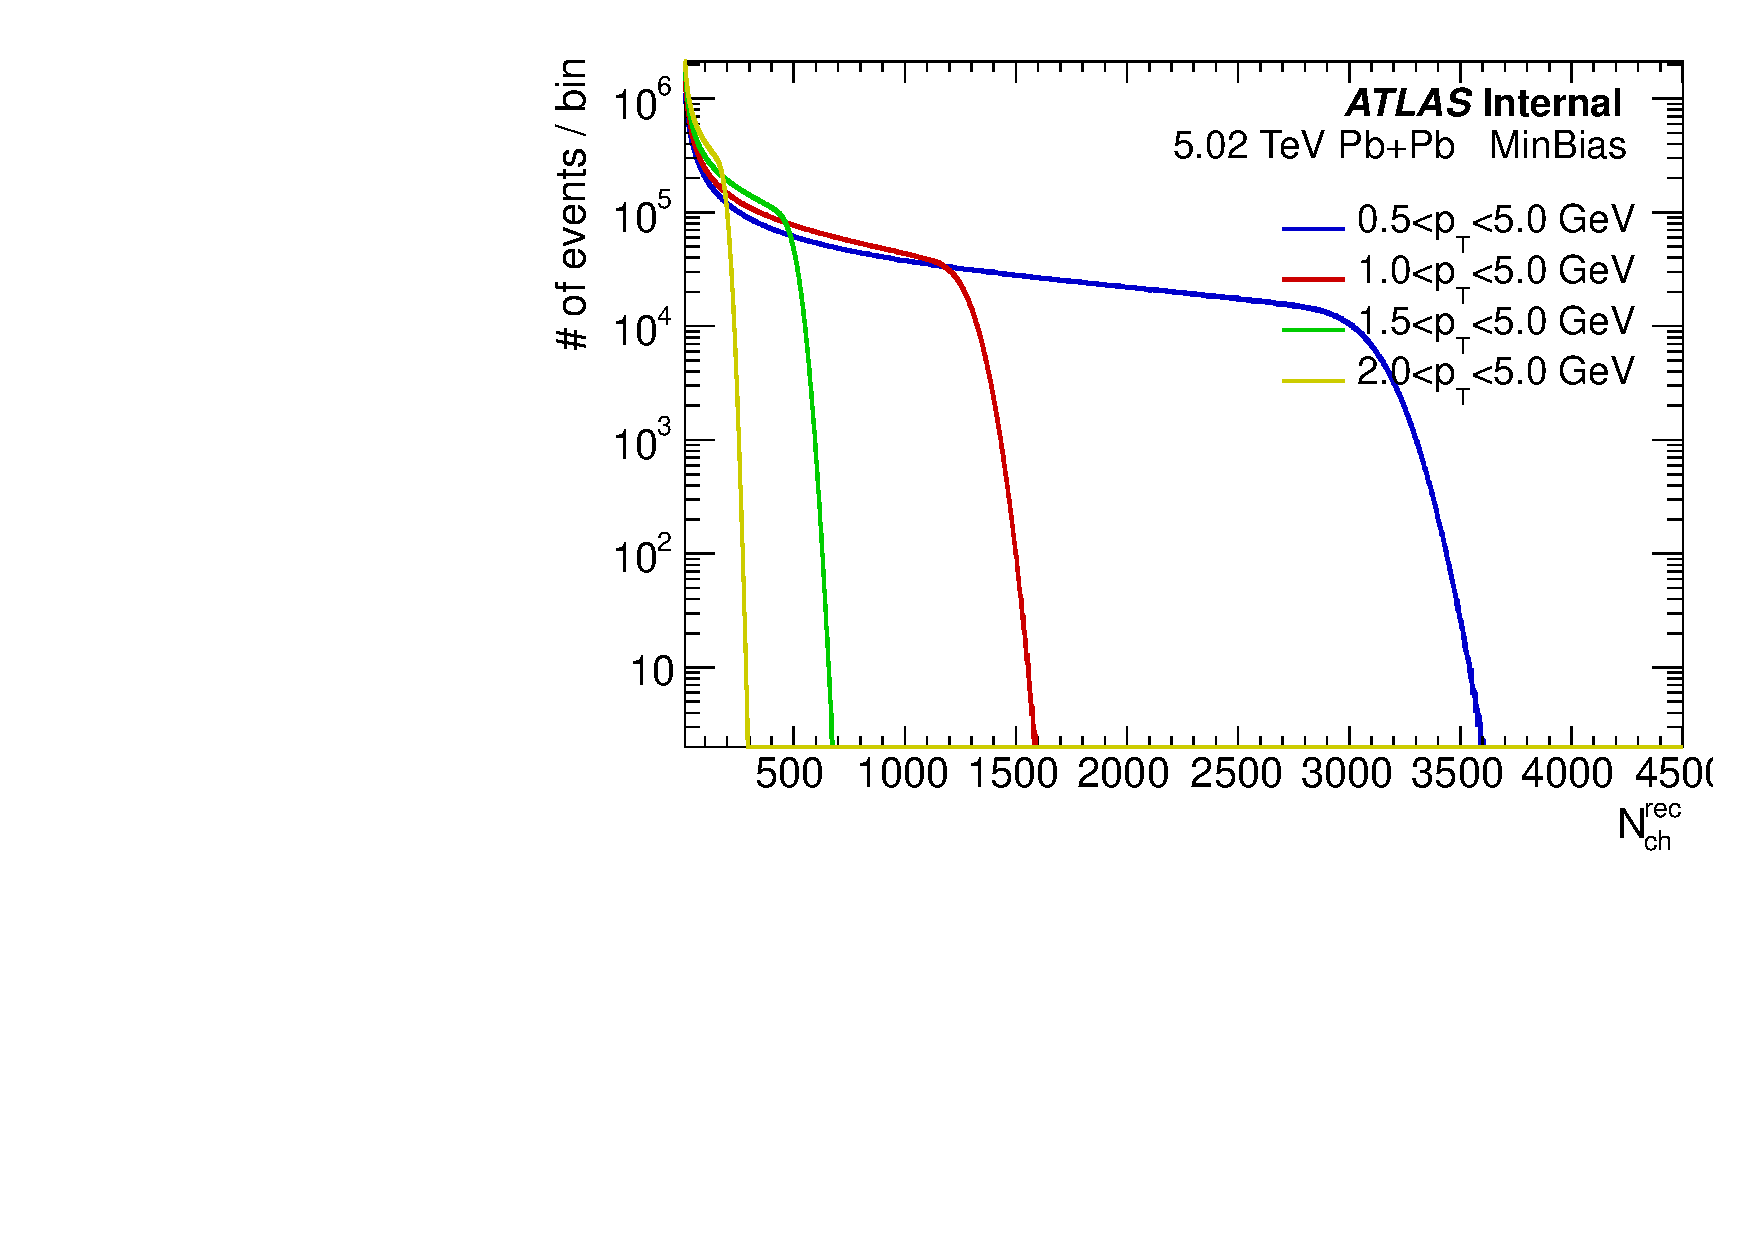
\includegraphics[width=.75\linewidth]{figs/sec_ana/cumuPhase_nTrkPt.pdf}
\caption{Distribution of reconstructed tracks from different $p_\text{T}$ ranges.}
\label{fig:cumuAna_PHASE_pt}
\end{figure}
To get an idea of how many particles are included with different $p_\text{T}$ cuts, Fig.~\ref{fig:cumuAna_PHASE_pt} shows the distributions of reconstructed tracks $N_{ch}^{rec}$ from different $p_\text{T}$ ranges. For $0.5<p_\text{T}<5.0$ GeV, the $N_{ch}^{rec}$ extends to 3600, while for the highest $p_\text{T}$ cut $2.0<p_\text{T}<5.0$ GeV, the largest $N_{ch}^{rec}$ is less than 300. This means that the statistical errors for the highest $p_\text{T}$ cut will be quite large.

In the standard cumulant method, all the particles have $-2.5<\eta<2.5$, while in the subevent method, the subevent is defined based on $\eta$:
\begin{itemize}
\item Subevent $a$: particles from $-2.5/3<\eta<2.5/3$;
\item Subevent $b$: particles from $-2.5<\eta<-2.5/3$;
\item Subevent $c$: particles from $2.5/3<\eta<2.5$;
\end{itemize}
where additional $\eta$ gaps can be applied between subevent $a$ and $b(c)$ to further suppress the long-range non-flow correlations.

\begin{figure}[H]
\centering
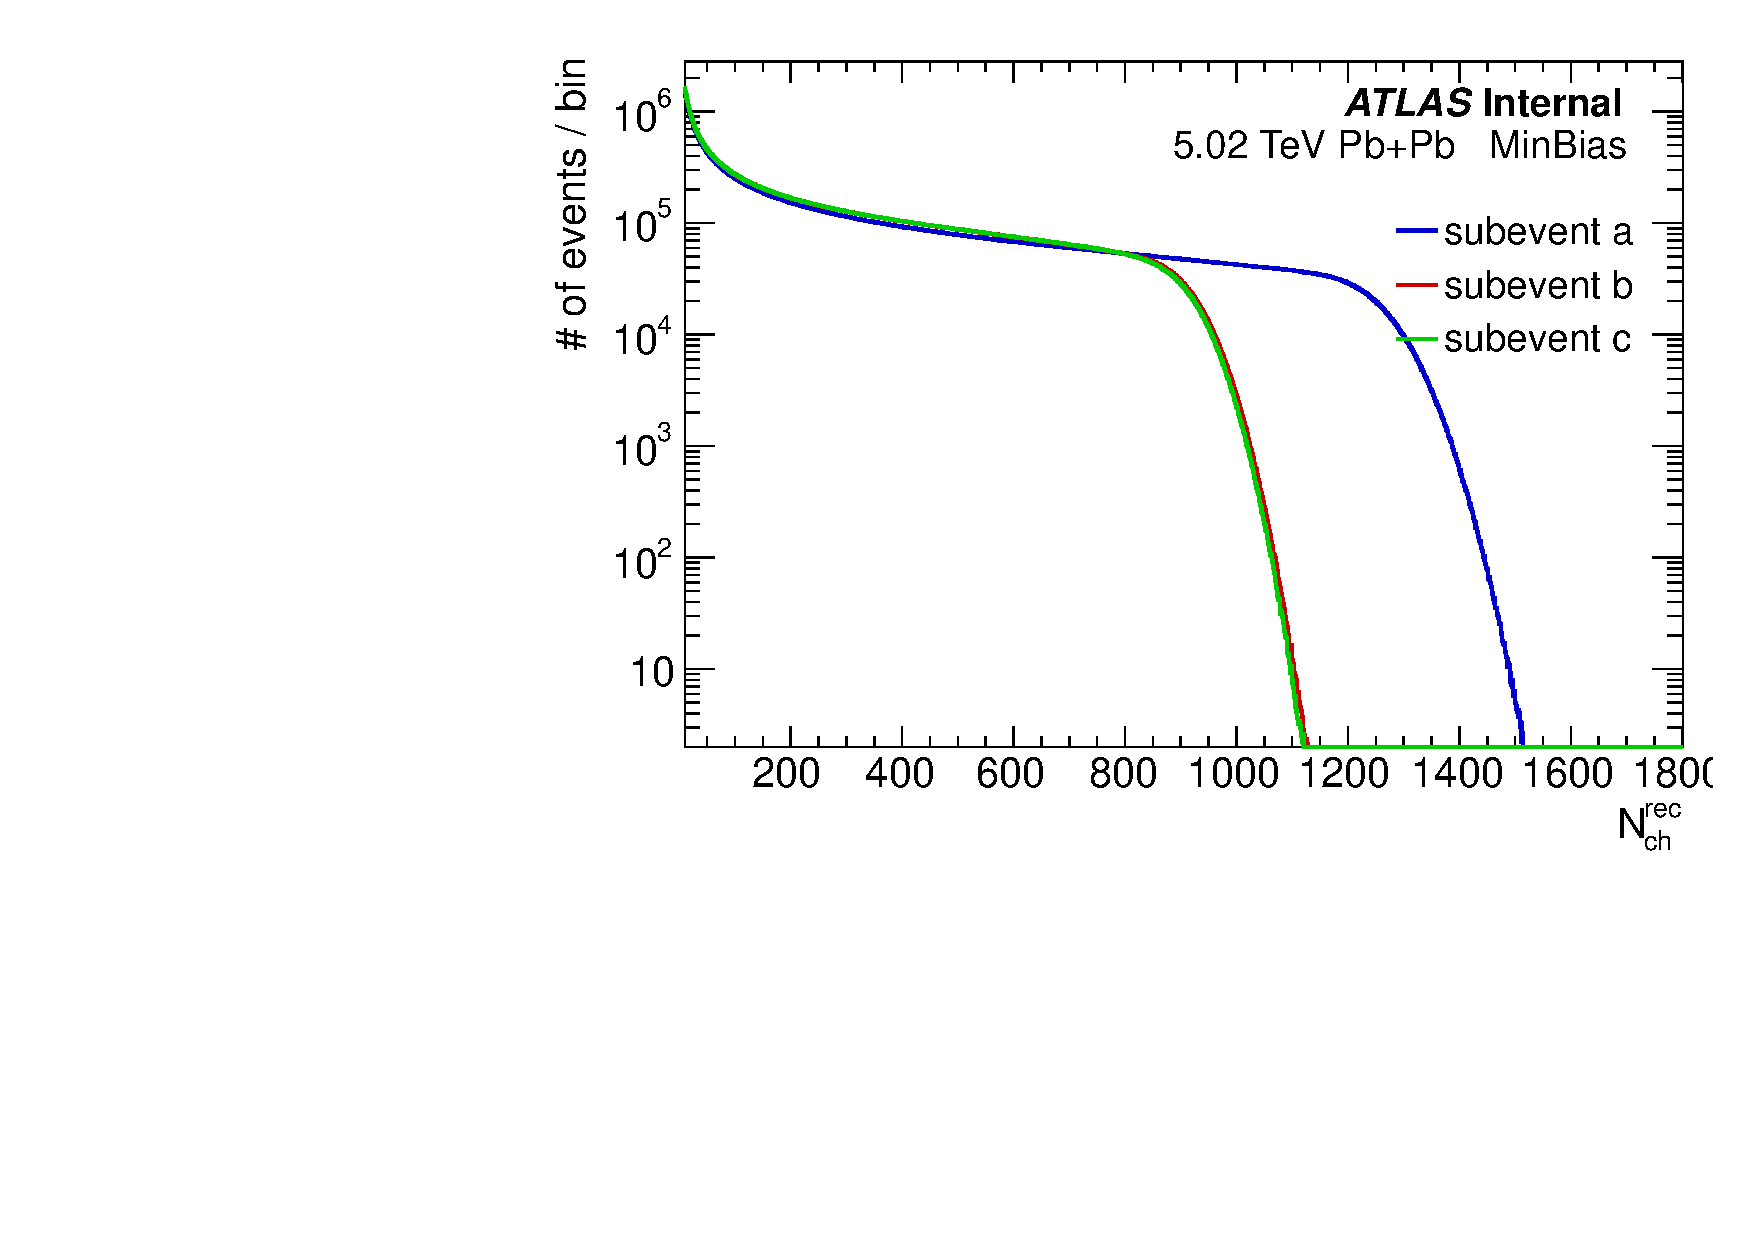
\includegraphics[width=.75\linewidth]{figs/sec_ana/cumuPhase_nTrkSub.pdf}
\caption{Distribution of reconstructed tracks from different $\eta$ ranges (subevents).}
\label{fig:cumuAna_PHASE_sub}
\end{figure}
Fig.~\ref{fig:cumuAna_PHASE_sub} shows the distribution of reconstructed tracks from different $\eta$ ranges, which are defined as subevent $a$, $b$ and $c$. $N_{ch}^{rec}$ is largest in subevent $a$ with $-2.5/3<\eta<2.5/3$, mainly due to two reasons: truth $N_{ch}$ slightly decreases as $|\eta|$ grows and the tracking efficiency also decrease at large $|\eta|$. Meanwhile, $N_{ch}^{rec}$ from subevent $b$ and $c$ are slightly different, which originates from the facts that: $1)$ mean of $z$ position of primary vertex is slightly shifted to the negative side, $2)$ tracking efficiency is not symmetric between positive and negative $\eta$.



\subsection{Trigger weighting}
Events in this analysis are collected by two minimum bias triggers and multiple UCC triggers. The statistics of collected events are shown in the left panel of Fig.~\ref{fig:ana_evtWght}, where the UCC triggers greatly enhanced the statistics in the region of FCal $E_\text{T}>4.2$ TeV. However, such enhancement will introduce potential bias when calculating cumulants in the event class defined by $N_{ch}^{rec}$. 

\begin{figure}[H]
\centering
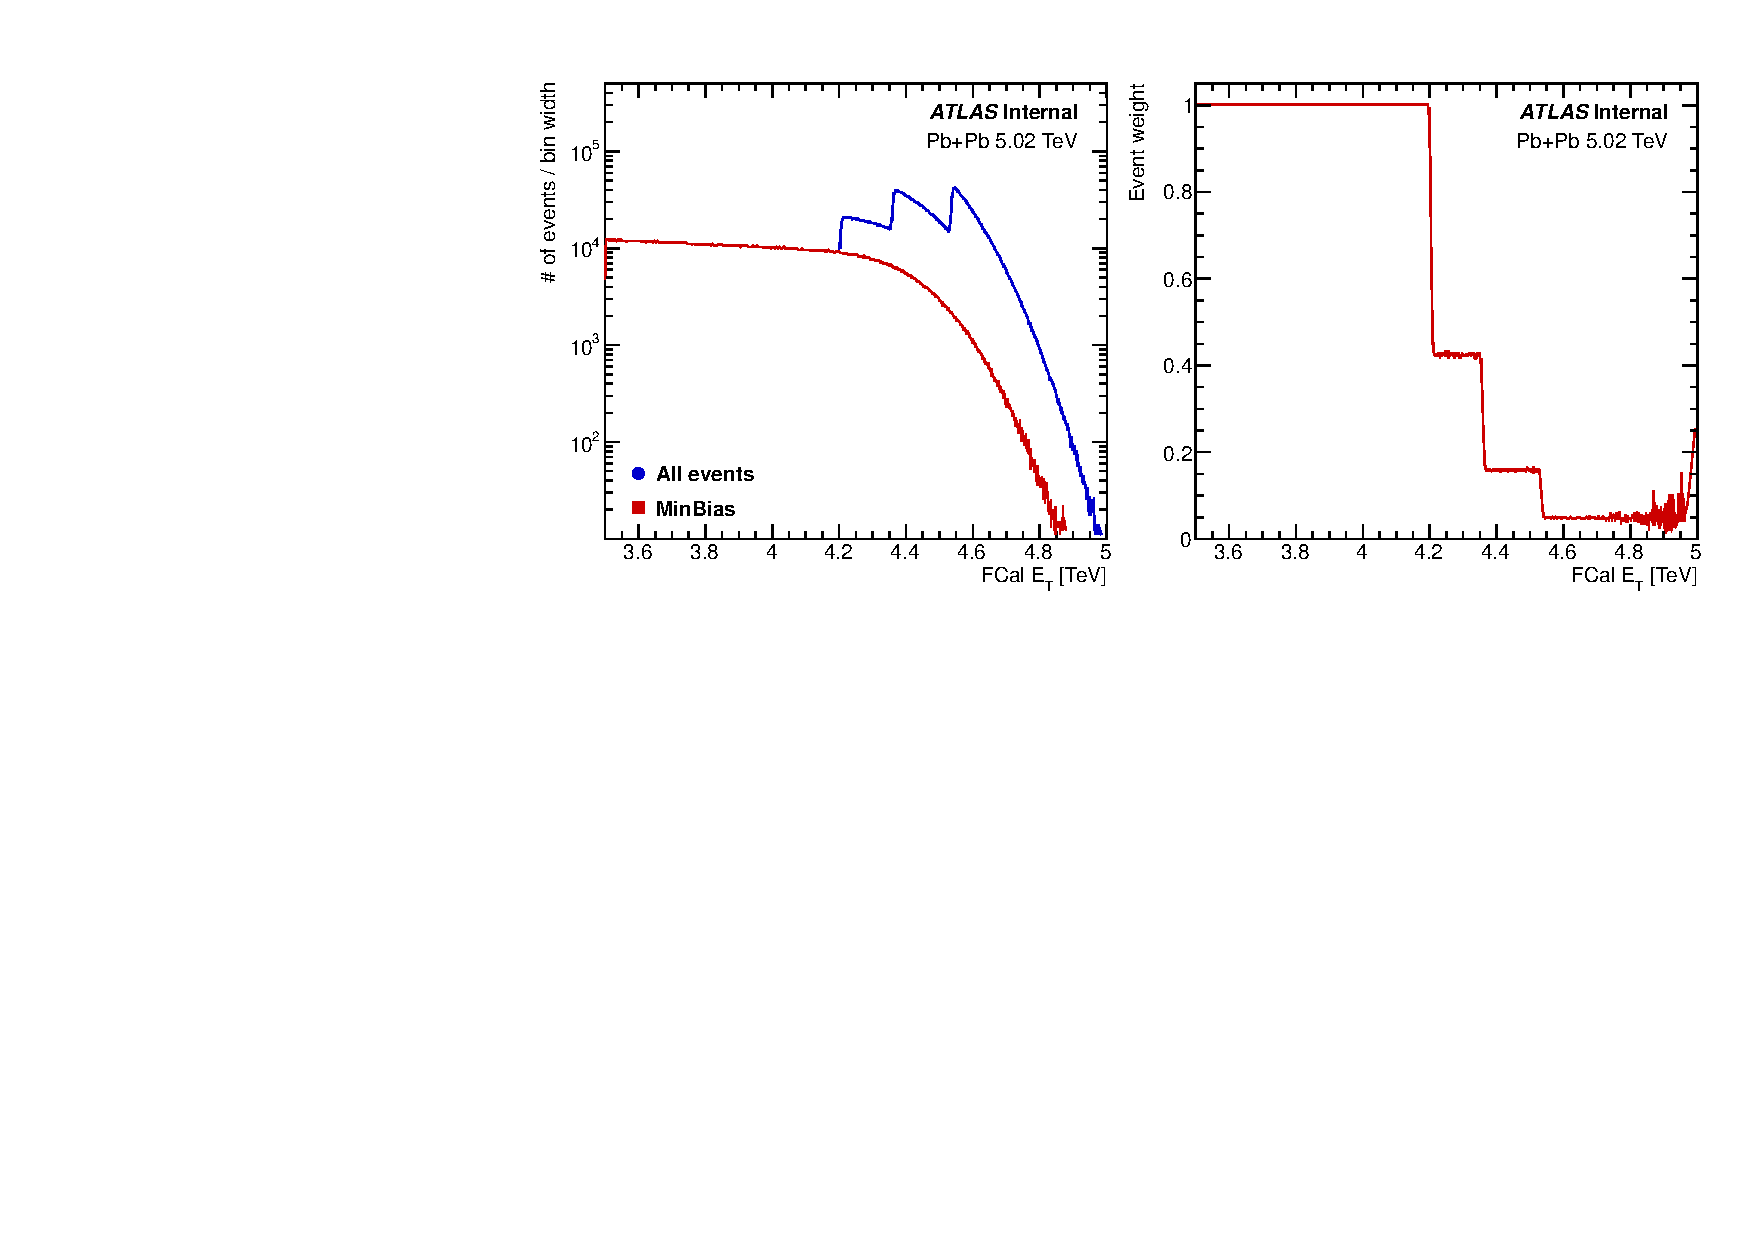
\includegraphics[width=.9\linewidth]{figs/sec_ana/trig_weight.pdf}
\caption{Additional event weights applied in order to properly include the UCC events.}
\label{fig:ana_evtWght}
\end{figure}

To properly include the events that passed UCC trigger, an event weight $w_{trig}$ has been applied to the $\lr{corr_{n}\{2k\}}$ calculation:
\begin{equation}
w_{trig}\equiv \frac{\text{events passed MinBias}}{\text{event passed MinBias and UCC}}
\end{equation}
where $w_{trig}$ is only estimated as a function of FCal $E_\text{T}$, as shown in the right panel of Fig.~\ref{fig:ana_evtWght}. $w_{trig}$ equals 1 for minimum-bias events and it lowers to three steps as FCal $E_\text{T}$ increases.

\begin{figure}[H]
\centering
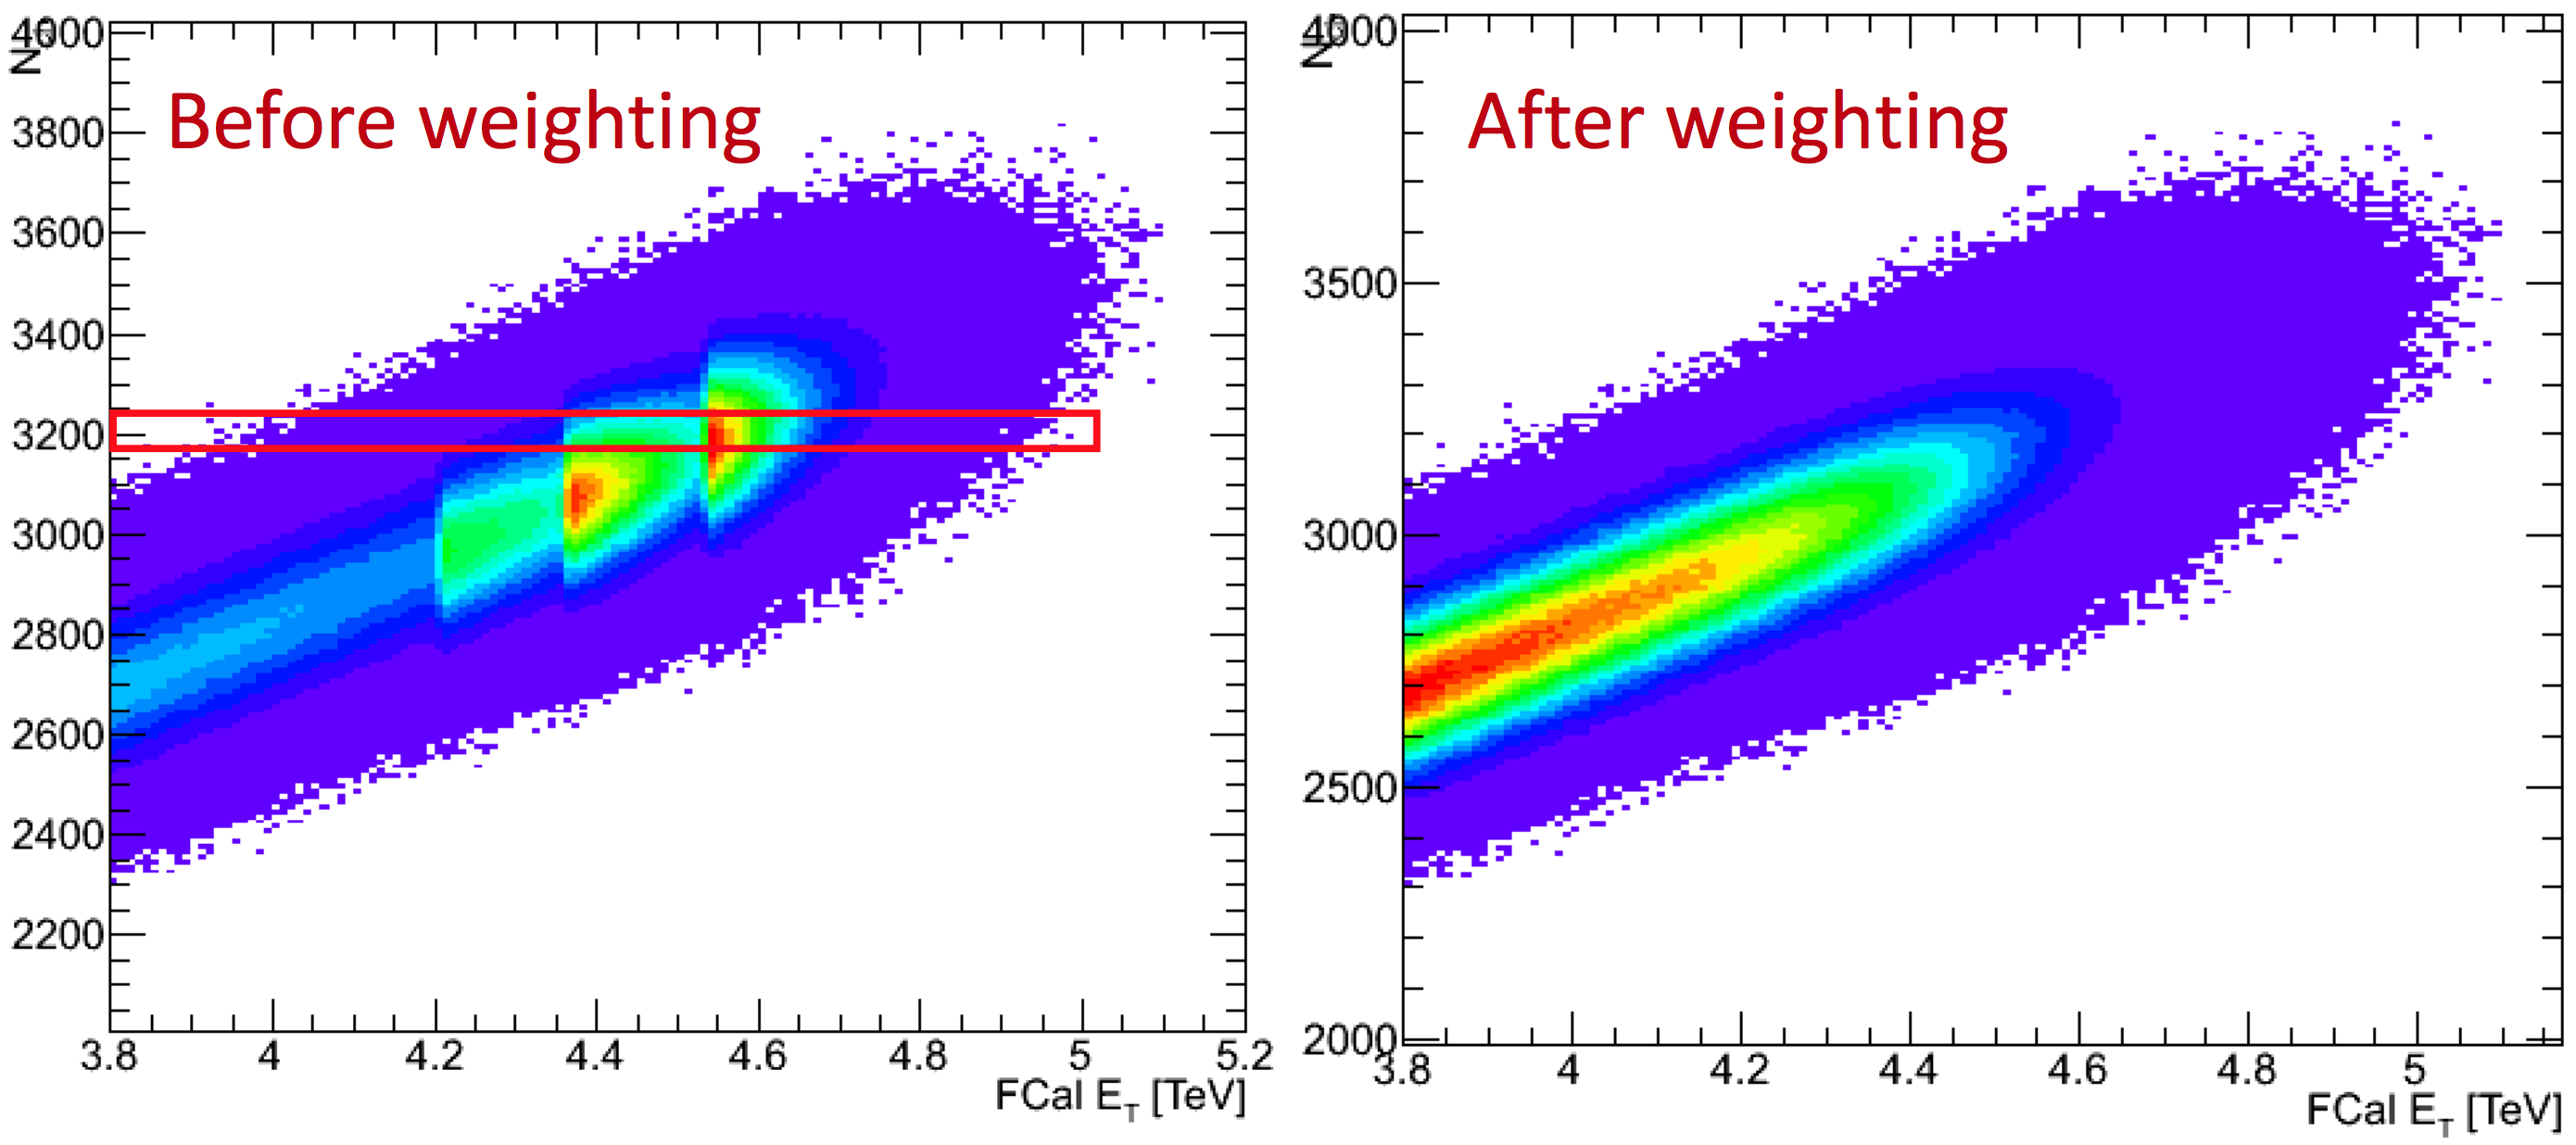
\includegraphics[width=.9\linewidth]{figs/sec_ana/evtWeight_comp.png}
\caption{Correlation between FCal sum $E_T$ and reconstructed tracks $N_{ch}^{rec}$, before (left) and after (right) applying the UCC trigger weights.}
\label{fig:ana_evtWght_comp}
\end{figure}
As one demonstration of how this event weight works, the correlation between FCal $E_\text{T}$ and number of reconstructed tracks $N_{ch}^{rec}$ is shown in Fig.~\ref{fig:ana_evtWght_comp}. Before $w_{trig}$ is applied, enhancement of statistics is observed in the large FCal $E_\text{T}$ region, while after applying $w_{trig}$, the minimum-bias + UCC distribution behaves just like the minimum-bias events as expected.



\subsection{Flattening procedure}
In heavy ion collisions, since the event plane angle fluctuates randomly event-by-event, the particle $\phi$ angle distribution averaged over many events should be flat, and the discrepancy is denoted as the detector effects. From the Monte-Carlo sample, tracking efficiency and fakes can be estimated as a function of $\eta$ and $p_\text{T}$, but the residual detector effects in the $\phi$ plane needs further correction, and the procedure is named as "flattening".

\begin{figure}[H]
\centering
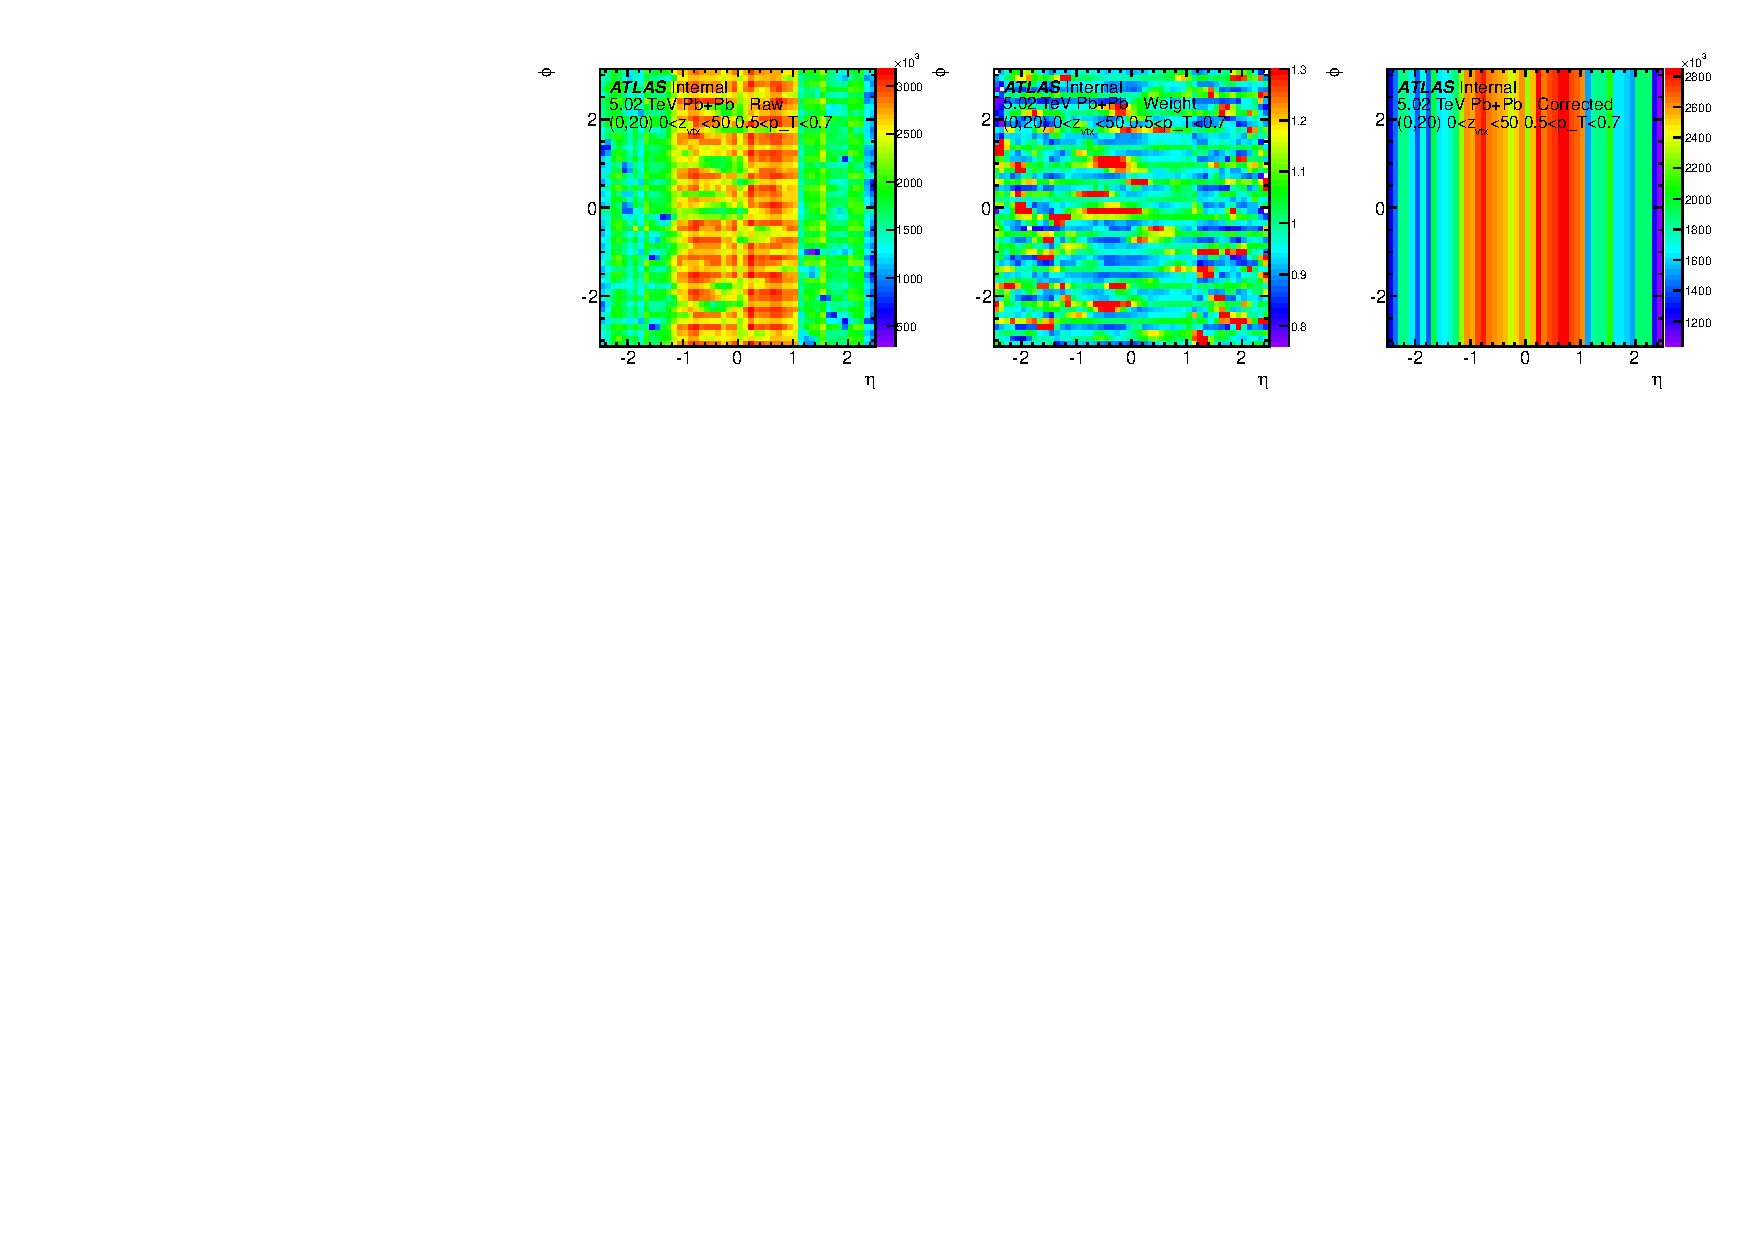
\includegraphics[width=.9\linewidth]{figs/sec_ana/cumuFlat_Cent0_Zvtx5_Chg0_Pt1.pdf}
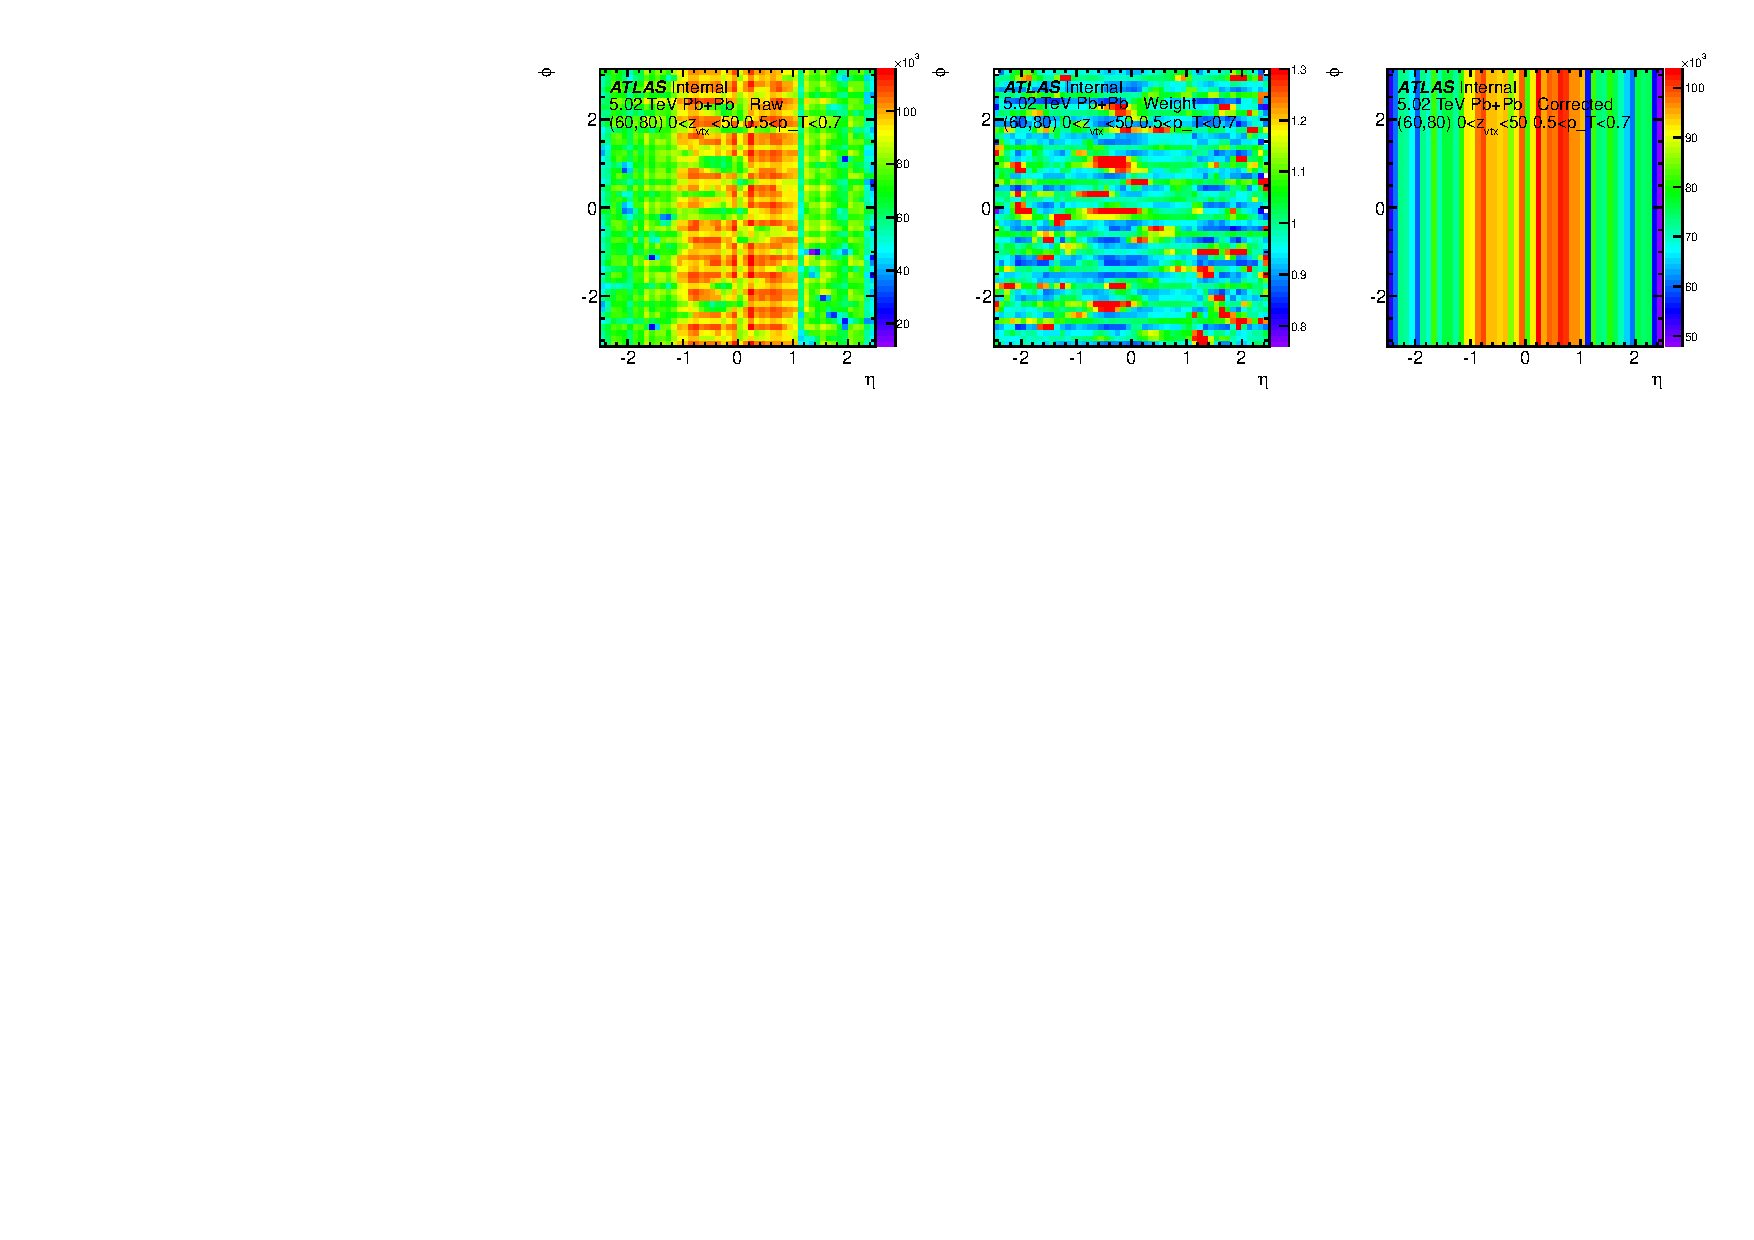
\includegraphics[width=.9\linewidth]{figs/sec_ana/cumuFlat_Cent3_Zvtx5_Chg0_Pt1.pdf}
\caption{Demonstration of flattening procedure in different centralities: top row is $0-20\%$ and bottom row is $60-80\%$. Left column are the raw $(\eta,\phi)$ distributions, middle column are the estimated correction factor $w_{\phi}$, right column are the corrected $(\eta,\phi)$ distributions. }
\label{fig:cumuAna_FLAT_Cent}
\end{figure}
Left column of Fig.~\ref{fig:cumuAna_FLAT_Cent} shows the raw $(\eta,\phi)$ distribution without any correction, and several "holes" are clearly observed in the transverse plane. In order to correct this detector effect, the correction factor $w_\phi$ is defined as:
\begin{equation}
w_\phi(\eta,\phi)\equiv\frac{\lr{N(\delta\eta)}}{N(\delta\eta,\delta\phi)}
\end{equation}
where $N(\delta\eta,\delta\phi)$ is the number of particles in the small $(\eta,\phi)$ phase-space window; and $\lr{N(\delta\eta)}$ is the mean number of particles in the small $\eta$ window averaged over the whole $\phi$ range. The middle panel gives an example of the $w_\phi(\eta,\phi)$: for the "holes" in raw $(\eta,\phi)$ distributions, $w_\phi$ is larger than 1. Right column shows the $(\eta,\phi)$ distribution after the correction, and as expected, for each narrow $\eta$ slice, the corrected $\phi$ distribution is uniform. This correction $w_{\phi}$ will be applied as the particle weight when calculating the $\lr{corr_{n}\{2k\}}$.

Since the detector effect depends on the occupancy of the detector, $w_\phi$ is evaluated in different centrality ranges. Fig.~\ref{fig:cumuAna_FLAT_Cent} shows a comparison between centrality $0-20\%$ and $60-80\%$. The correction factors are not identical, but very similar between the two centralities.

\begin{figure}[H]
\centering
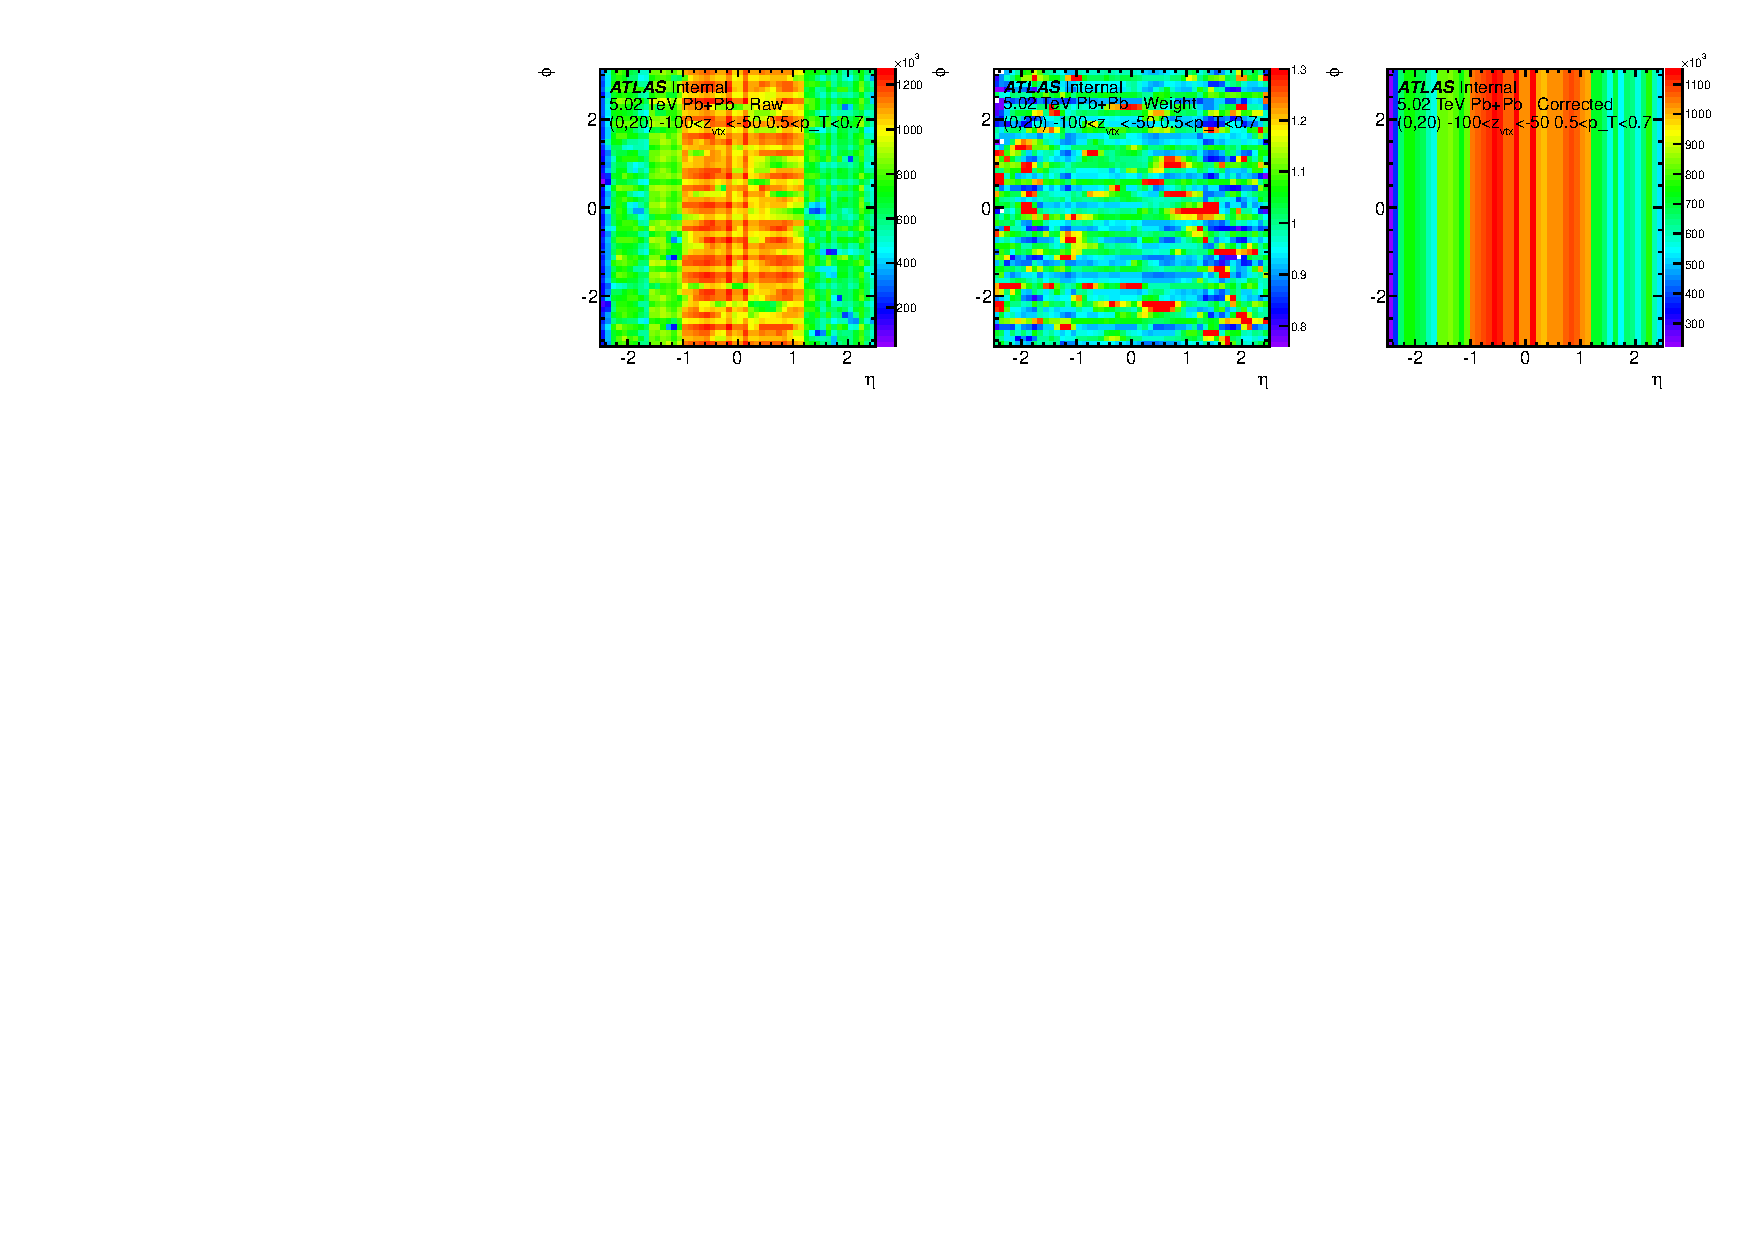
\includegraphics[width=.9\linewidth]{figs/sec_ana/cumuFlat_Cent0_Zvtx3_Chg0_Pt1.pdf}
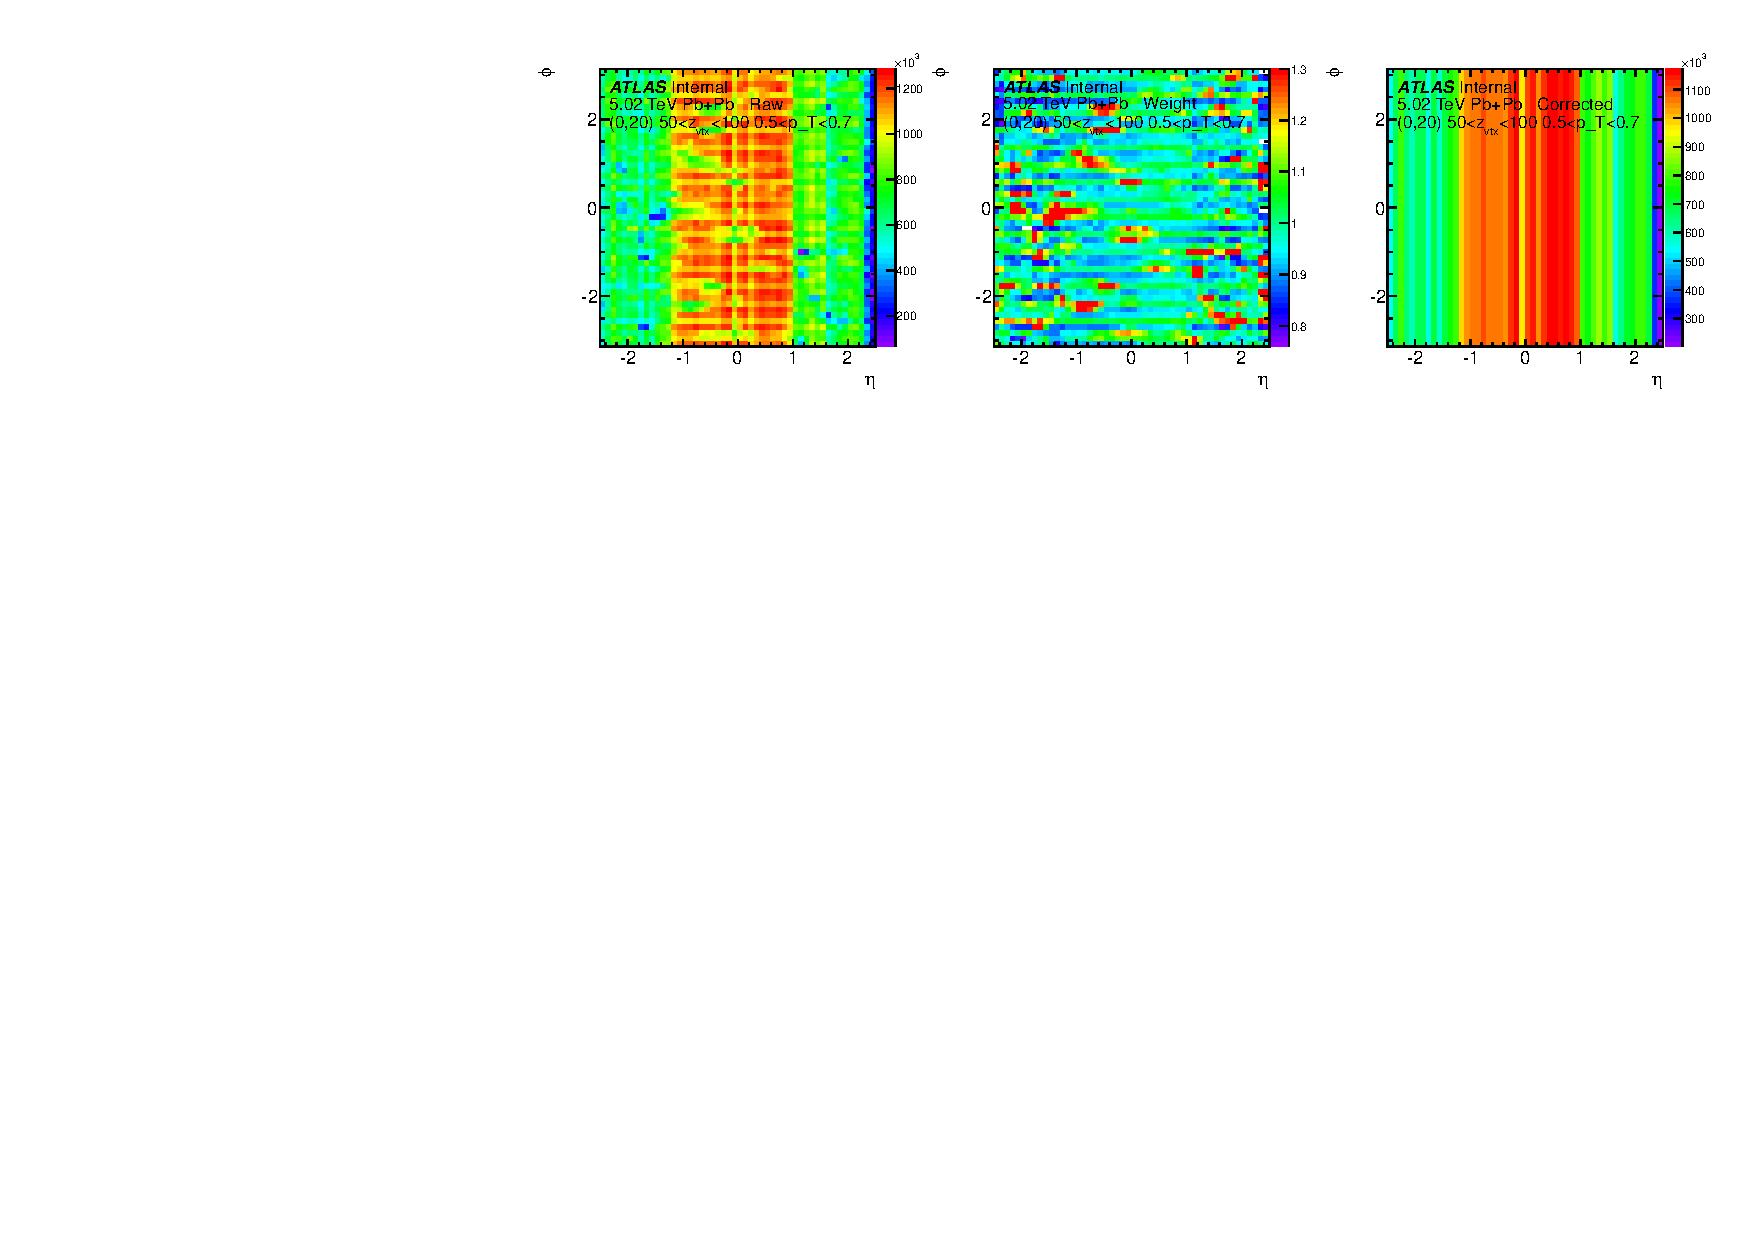
\includegraphics[width=.9\linewidth]{figs/sec_ana/cumuFlat_Cent0_Zvtx6_Chg0_Pt1.pdf}
\caption{Demonstration of flattening procedure in different $z_{vtx}$ ranges: top row is from -100 mm$<z_{vtx}<$-50 mm and bottom row is from 50 mm$<z_{vtx}<$100 mm. Left column are the raw $(\eta,\phi)$ distributions, middle column are the estimated correction factor $w_{\phi}$, right column are the corrected $(\eta,\phi)$ distributions.}
\label{fig:cumuAna_FLAT_Zvtx}
\end{figure}

\begin{figure}[H]
\centering
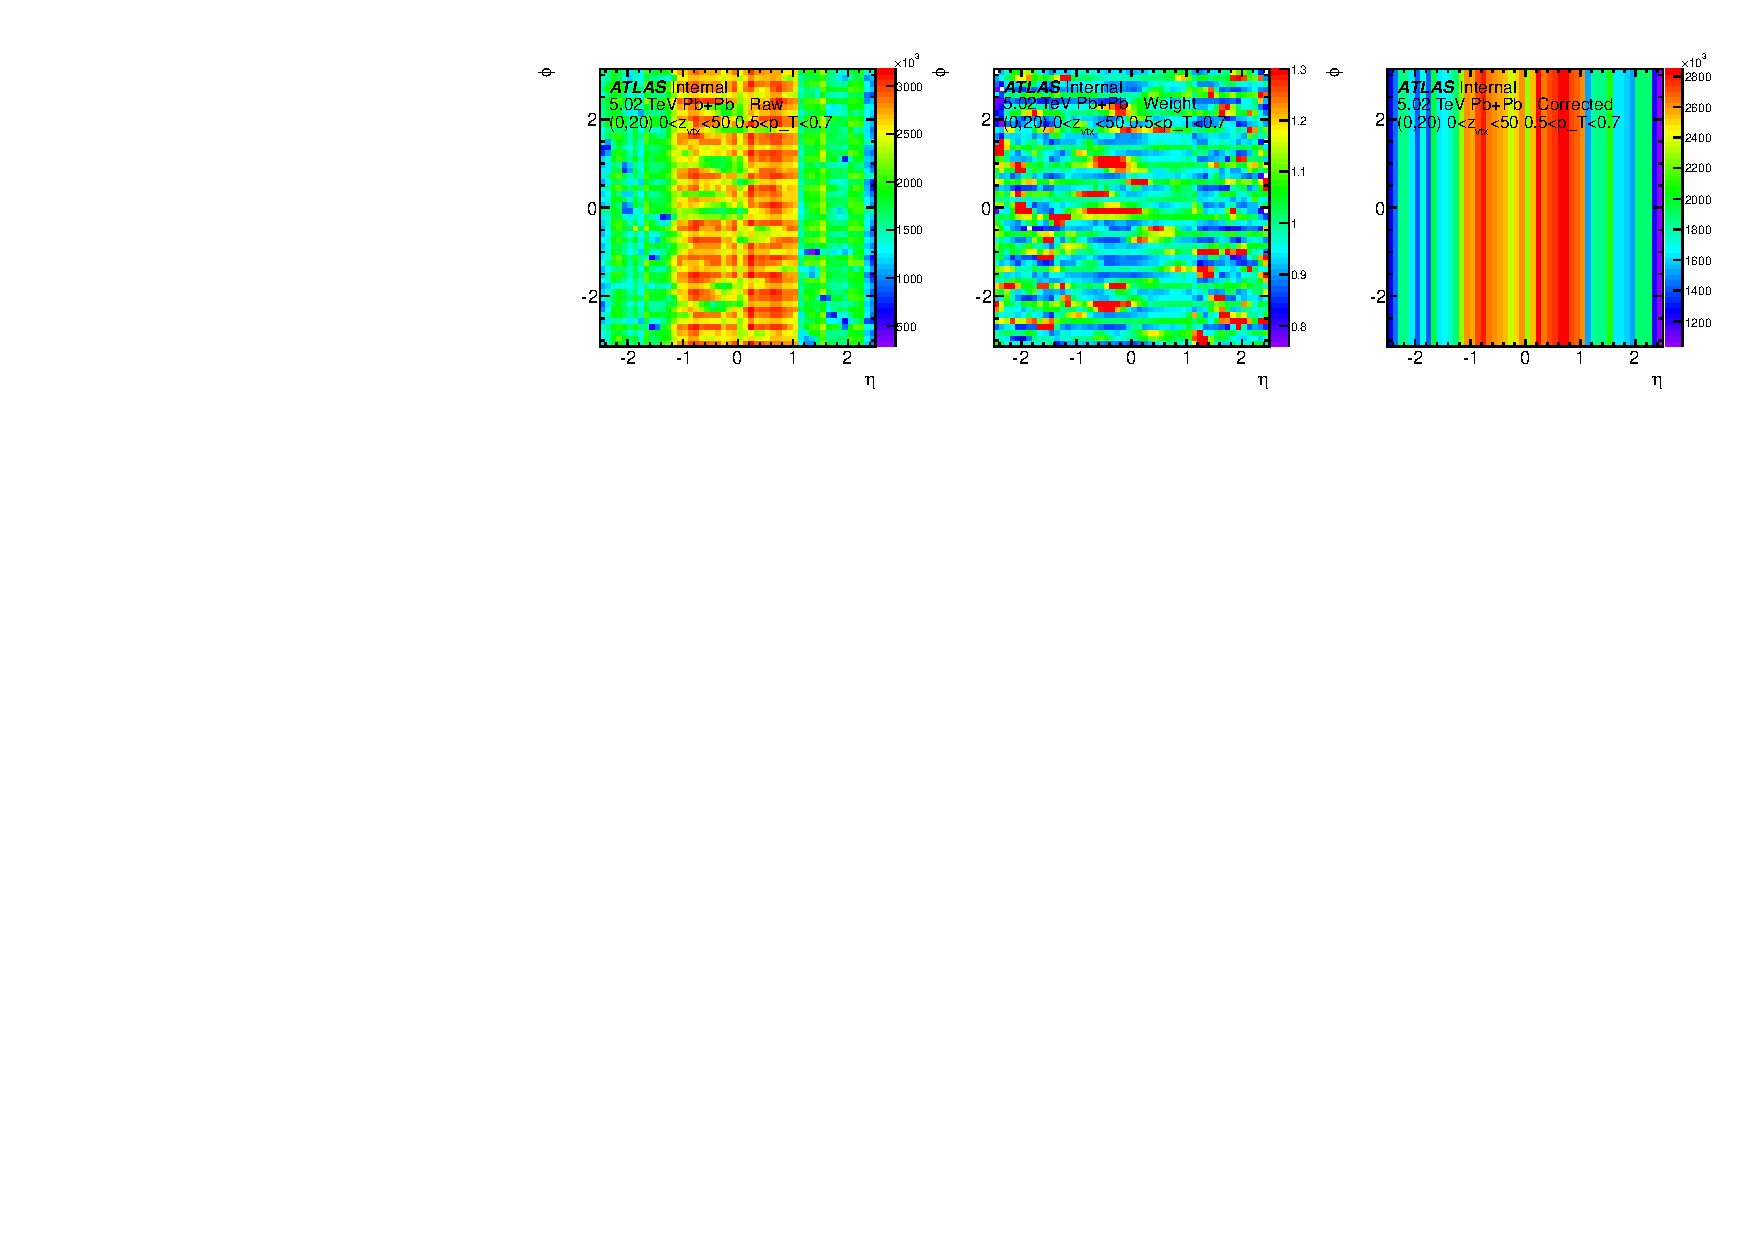
\includegraphics[width=.9\linewidth]{figs/sec_ana/cumuFlat_Cent0_Zvtx5_Chg0_Pt1.pdf}
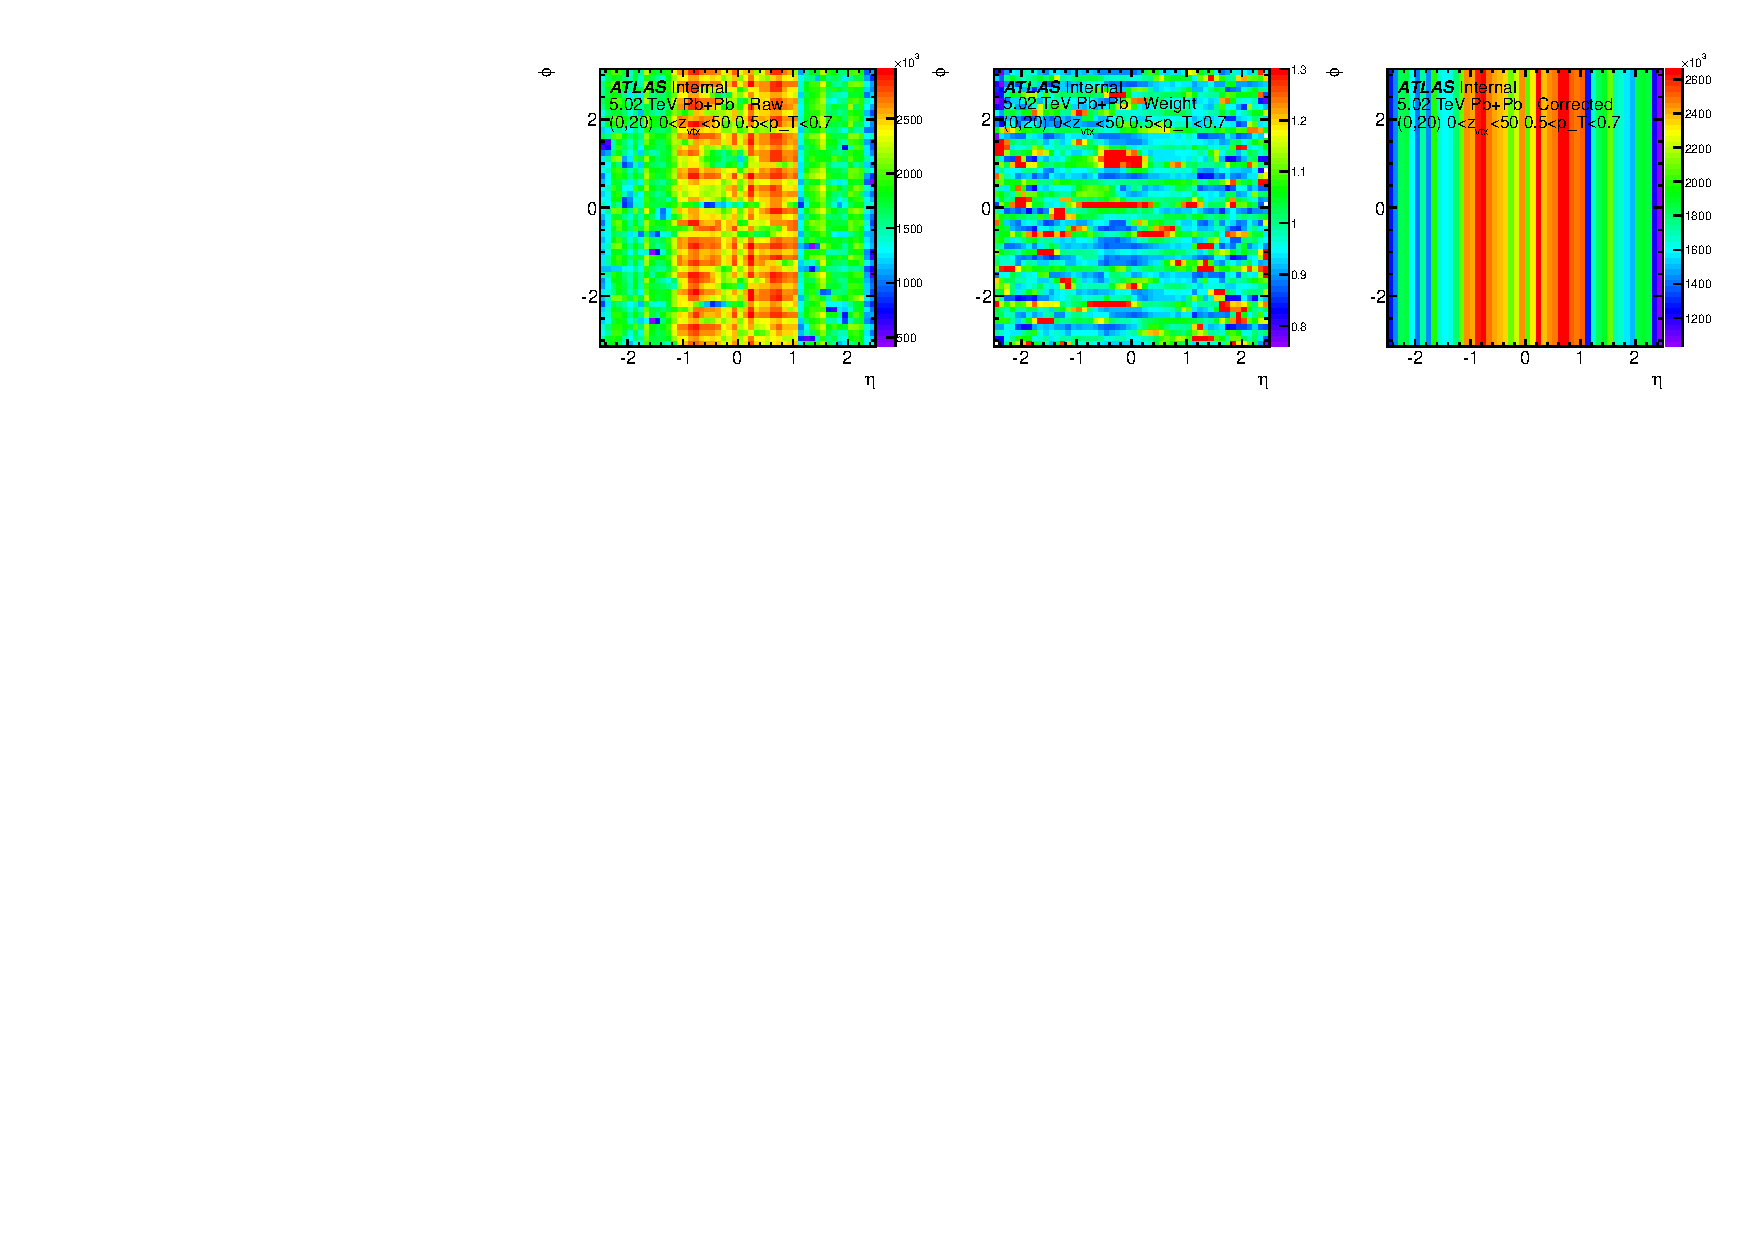
\includegraphics[width=.9\linewidth]{figs/sec_ana/cumuFlat_Cent0_Zvtx5_Chg1_Pt1.pdf}
\caption{Demonstration of flattening procedure with particles of different charges: top row is for negative-charged particles and bottom row is for positive-charged particles. Left column are the raw $(\eta,\phi)$ distributions, middle column are the estimated correction factor $w_{\phi}$, right column are the corrected $(\eta,\phi)$ distributions.}
\label{fig:cumuAna_FLAT_Chg}
\end{figure}

\begin{figure}[H]
\centering
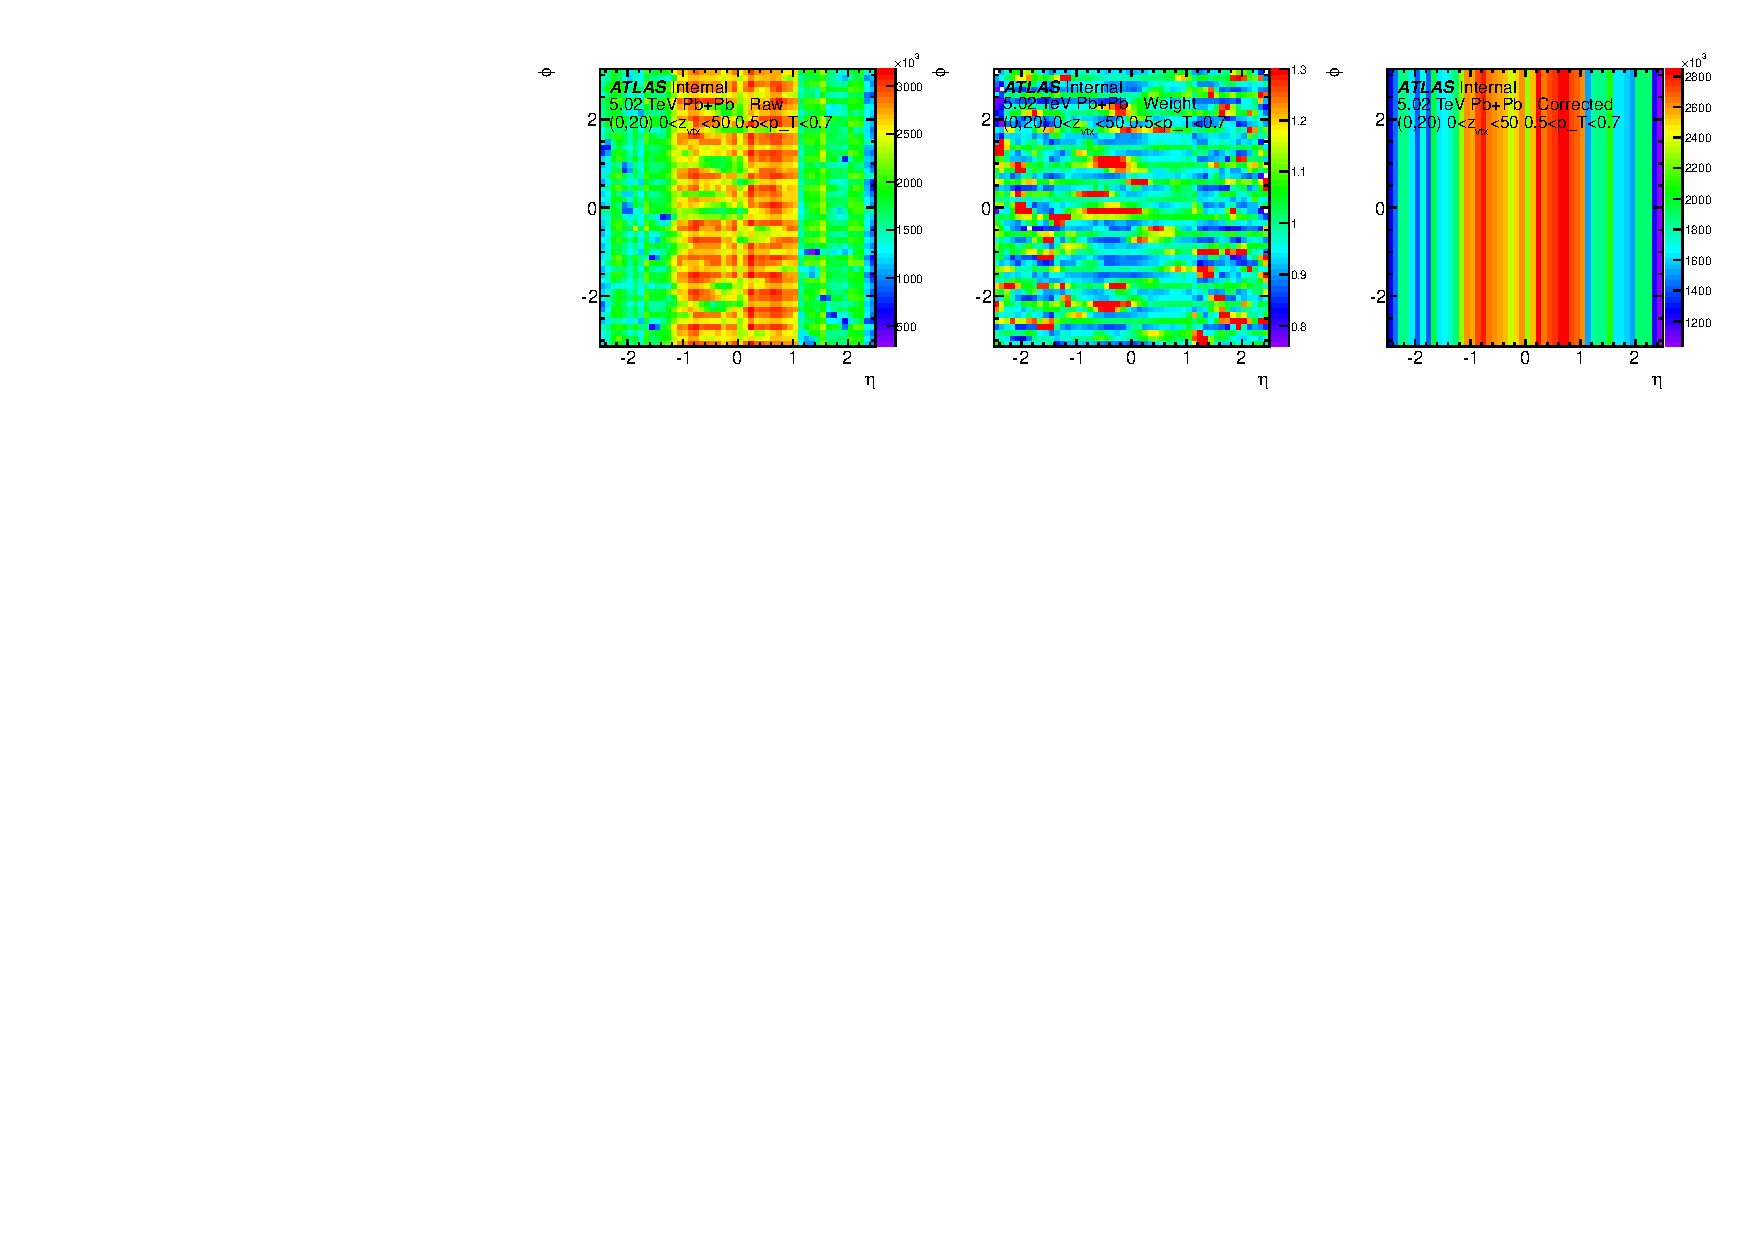
\includegraphics[width=.9\linewidth]{figs/sec_ana/cumuFlat_Cent0_Zvtx5_Chg0_Pt1.pdf}
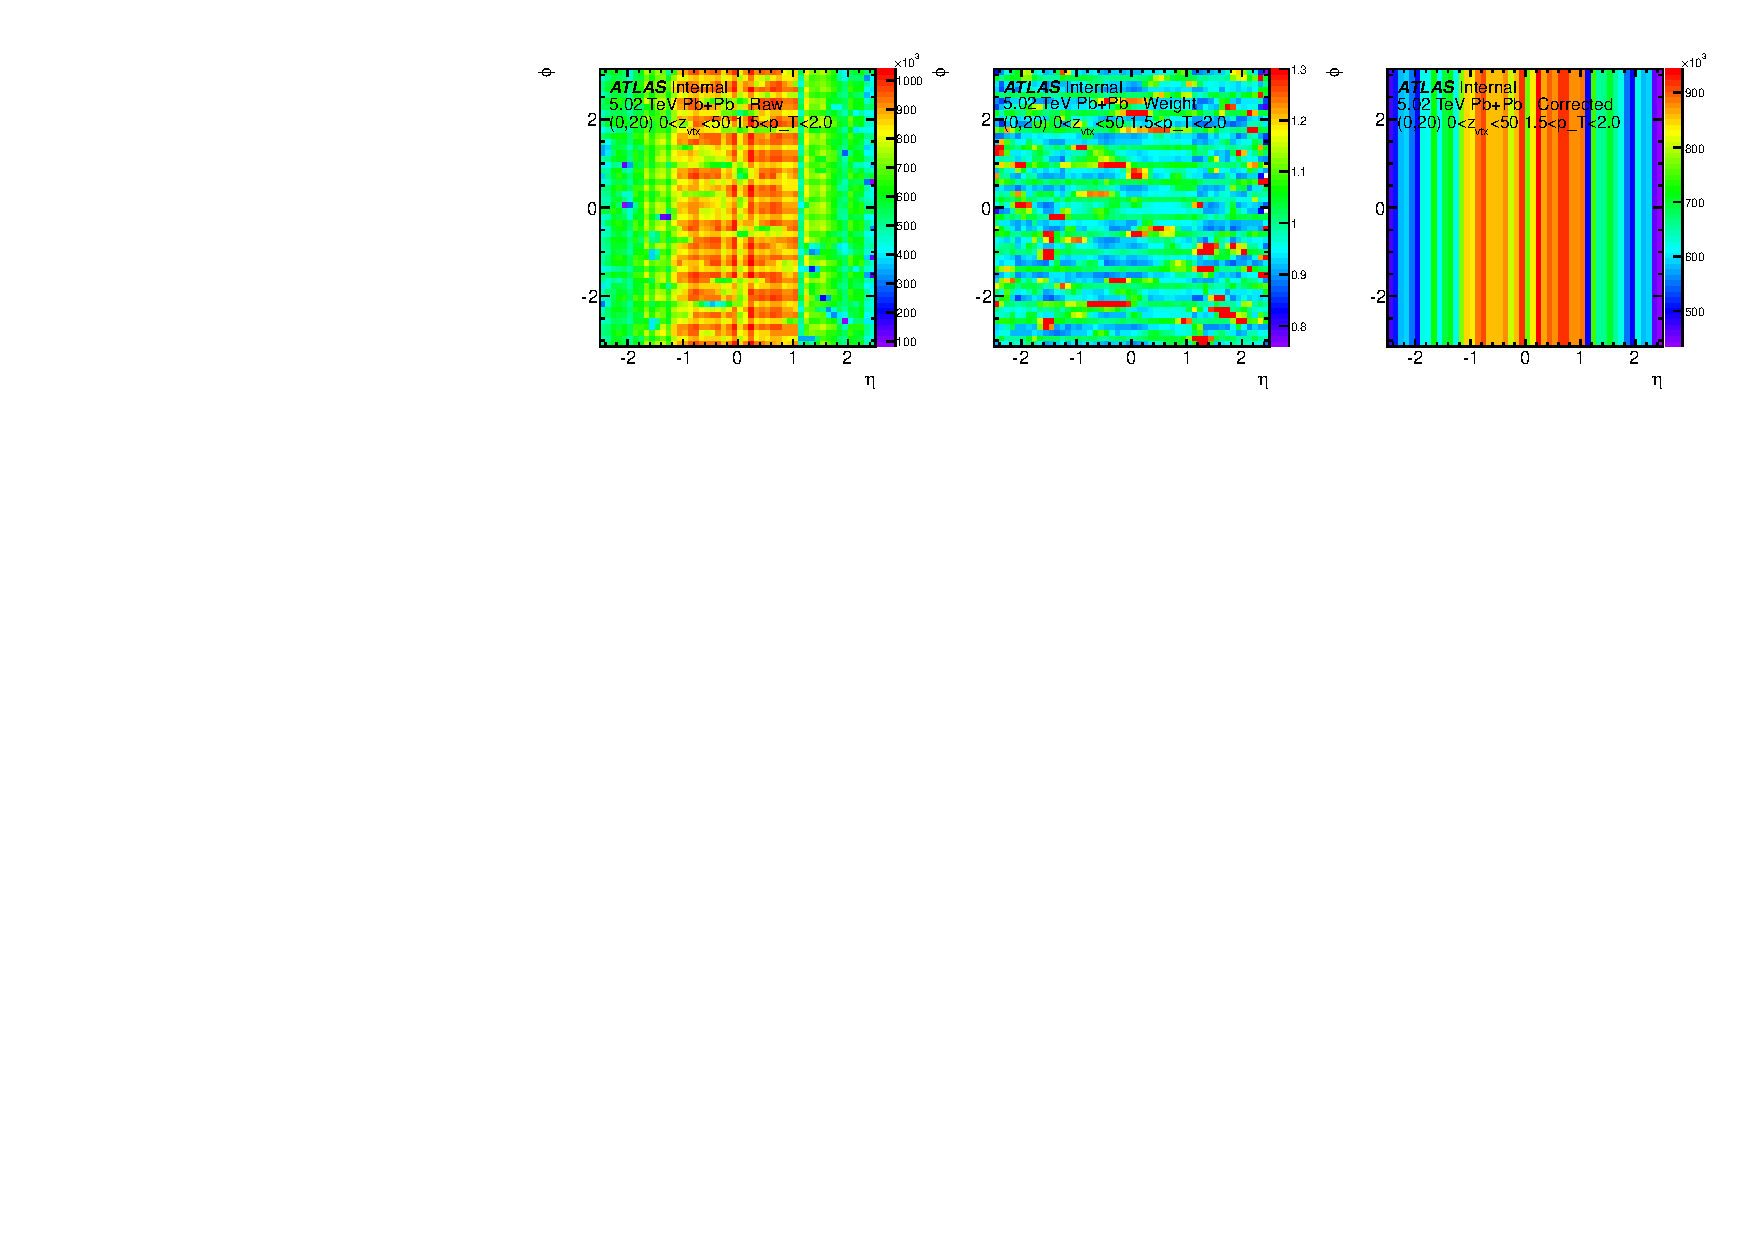
\includegraphics[width=.9\linewidth]{figs/sec_ana/cumuFlat_Cent0_Zvtx5_Chg0_Pt4.pdf}
\caption{Demonstration of flattening procedure with particles from different $p_\text{T}$ ranges: top row has $0.5<p_\text{T}<0.7$ GeV and bottom row has $1.5<p_\text{T}<2.0$ GeV. Left column are the raw $(\eta,\phi)$ distributions, middle column are the estimated correction factor $w_{\phi}$, right column are the corrected $(\eta,\phi)$ distributions. }
\label{fig:cumuAna_FLAT_Pt}
\end{figure}

In additional, the fluctuation of $z$ position of the primary vertex will cause the $N_{ch}$ distribution to shift in $\eta$. To compensate this effect, $w_\phi$ is also estimated in different $z_{vtx}$ ranges. Fig.~\ref{fig:cumuAna_FLAT_Zvtx} shows a comparison between -150 mm$<z_{vtx}<$-100 mm and 100 mm$<z_{vtx}<$150 mm. From the left column, it is clear that the $\eta$ distributions are shifted together with $z_{vtx}$ position, which means that a $z_{vtx}$-dependent $w_\phi$ correction is needed.

Furthermore, the $w_\phi$ corrections are also evaluated for negative- and positive-charged particles separately, as shown in Fig.~\ref{fig:cumuAna_FLAT_Chg}. From the raw distribution, differences have already been observed: there are slightly more holes for positive particles than negative ones.

In the end, Fig.~\ref{fig:cumuAna_FLAT_Pt} shows the comparison of $w_\phi$ estimated from particles in two different $p_\text{T}$ ranges: $0.3<p_\text{T}<0.5$ GeV and $1.5<p_\text{T}<2.0$ GeV. As a results, particles with higher $p_\text{T}$ are more uniformly distributed, which is consistent with the fact that tracking efficiency increases towards higher $p_\text{T}$.



\subsection{Event class}
Event-by-event multi-particle correlation $corr_{n}\{2k\}$ is averaged within bunch of similar events, which are denoted as event class. Since cumulant measures the flow fluctuation in certain event class, how event class is defined will have an effect on the cumulant magnitude. In previous ATLAS paper on cumulant in small systems, we have shown that even the sign of cumulant can change if the event class definition is changed. In this section, we will discuss the definition of event class in this analysis and its potential impact on the cumulant results.

Since flow in the final stage is strongly correlated with the eccentricity from the initial stage, an optimal quantity to model the eccentricity changing would be centrality, which reflects the overlapping region of the two nucleus. In heavy ion collision, since centrality is not a direct-measurable quantity, total transverse energy $E_\text{T}$ in the FCal detector is used as an indicator for centrality, which means the centrality percentile is calculated based on the FCal $E_\text{T}$ distribution (see the Dataset section for details). In this analysis, the default event class will be defined by centrality.

The following question is how large the event class bin width should be. In principle, narrower bin width is always preferred, since wider bin width will include events from different centralities, which can result in different flow fluctuation. However, there will be not enough events to calculate the higher order cumulants if the bin width is too narrow. In practice we choose $1\%$ centrality percentile as the default event class bin width.

To show that $1\%$ bin width will not introduce any bias to the measurement, we have also tested the following bin widths:
\begin{itemize}
\item Event class bin width: $2\%$;
\item Event class bin width: $5\%$;
\item Event class bin width: $10\%$;
\end{itemize}
and the results will be discussed in the systematic section.

As discussed in the methodology section, even though the event class bin width is only $1\%$ centrality, neighbouring bins will be merged together at the cumulant level to increase the statistics. Note that since the re-bin is performed on the cumulant, it does not change the underlying flow fluctuation.

The event class definition is specially treated in the ultra-central collision, simply because $1\%$ centrality bin width is not narrow enough to constrain the fluctuation of flow. Instead, the following event class criteria are used:
\begin{itemize}
\item Event class defined by FCal $E_\text{T}$, with bin width $=6$ GeV;
\item Event class defined by number of reconstructed tracks $N_{ch}^{rec}$, with $p_\text{T}$ range always $0.5<p_\text{T}<5.0$ GeV, no matter the $p_\text{T}$ range for the cumulant calculation. The bin width is 5 track;
\end{itemize}
where the purpose of the second criteria is to evaluate the flow fluctuation by changing the centrality definition, which will be discussed in the results section.

\begin{figure}[H]
\centering
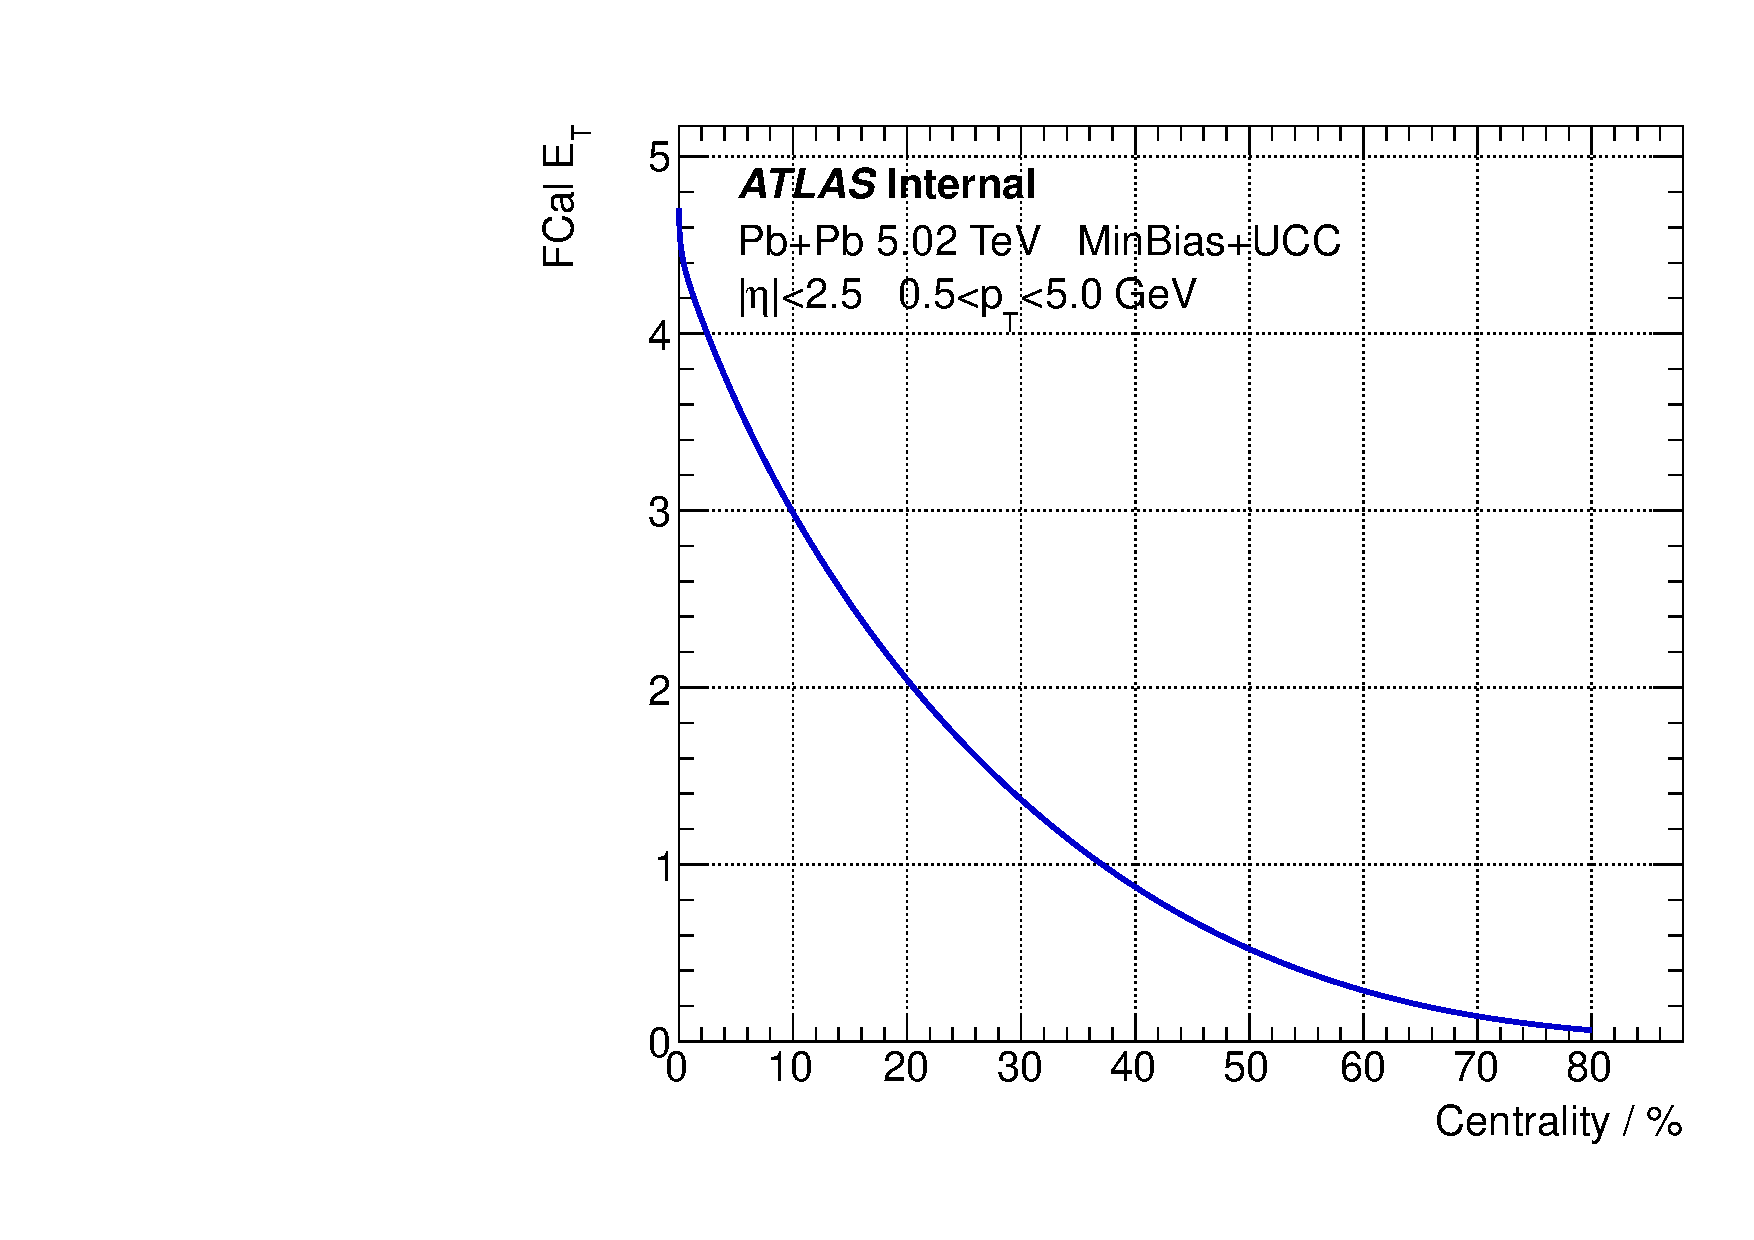
\includegraphics[width=.32\linewidth]{figs/sec_ana/cvtMap_cent_fcal.pdf}
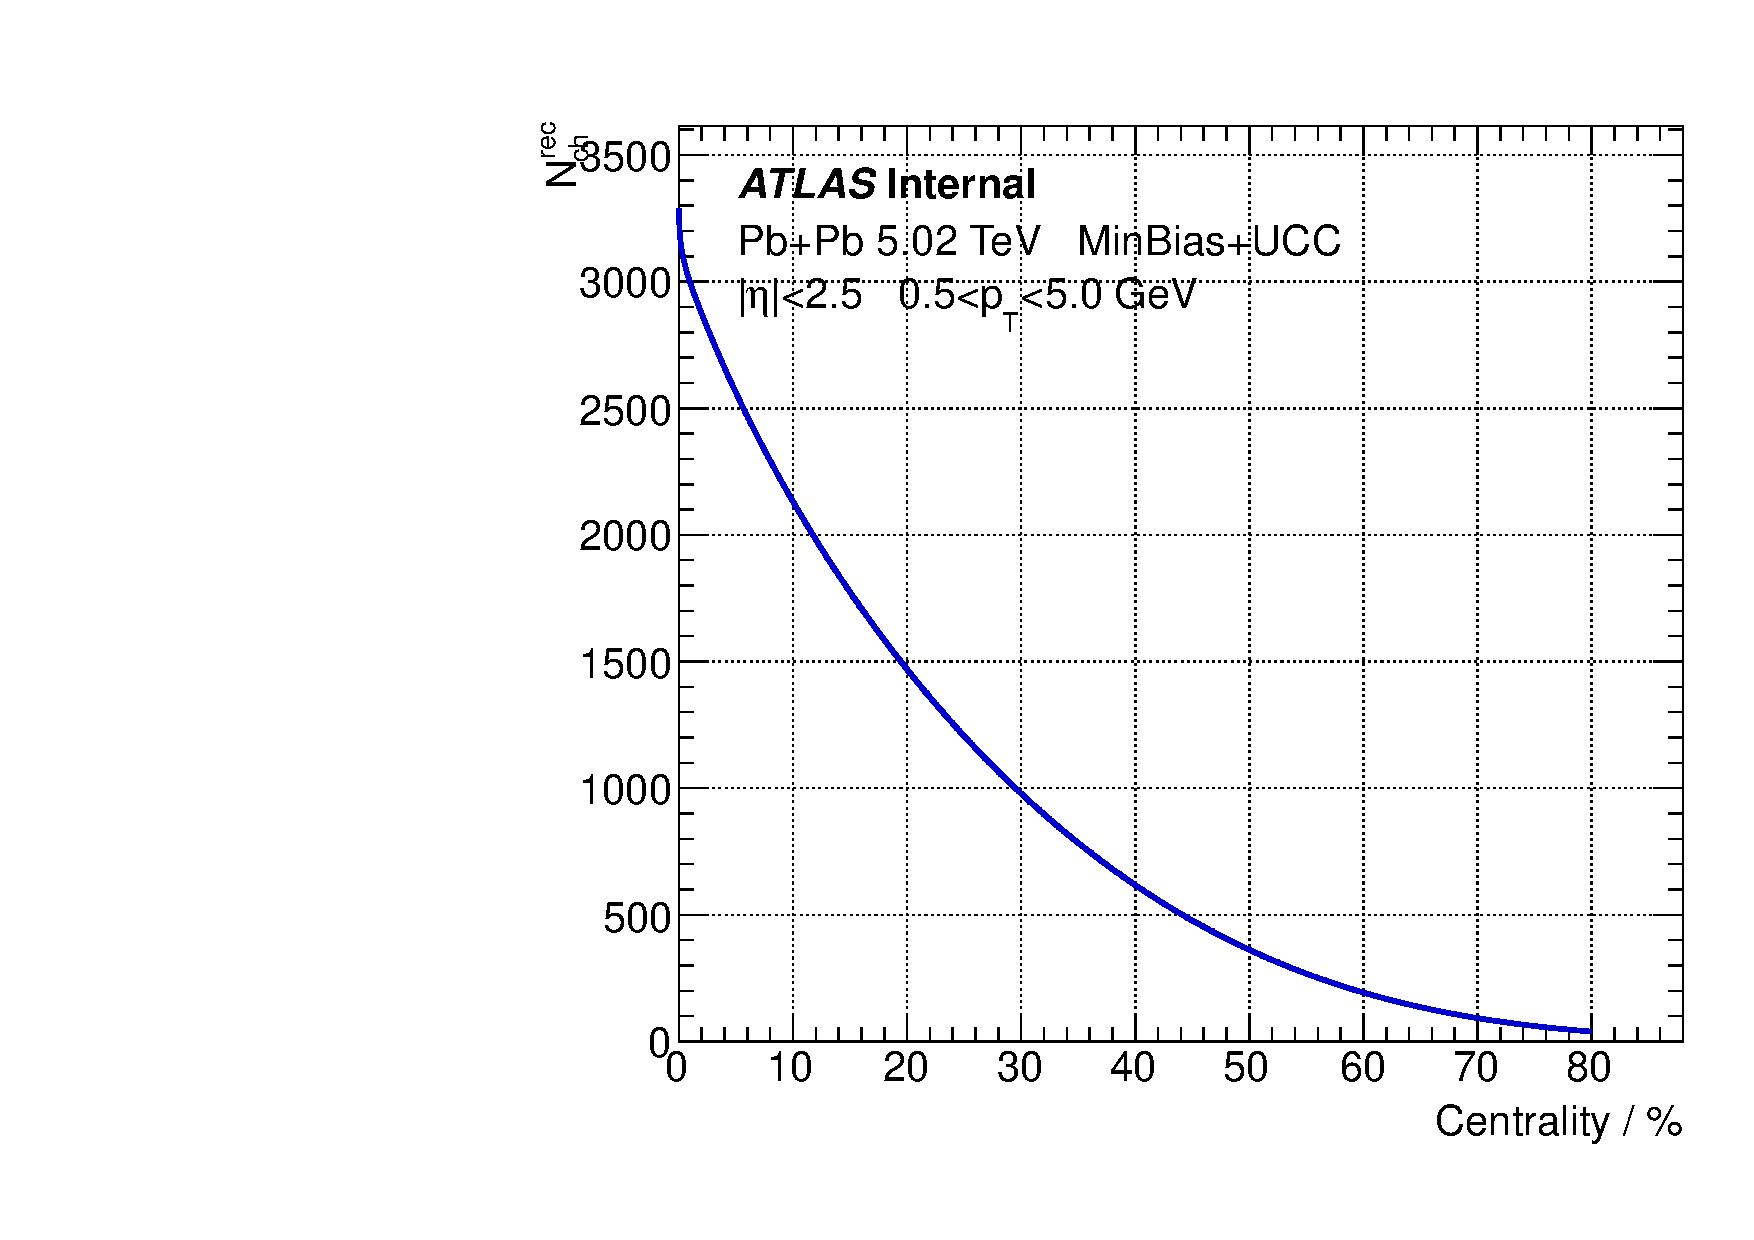
\includegraphics[width=.32\linewidth]{figs/sec_ana/cvtMap_cent_NchRec.pdf}
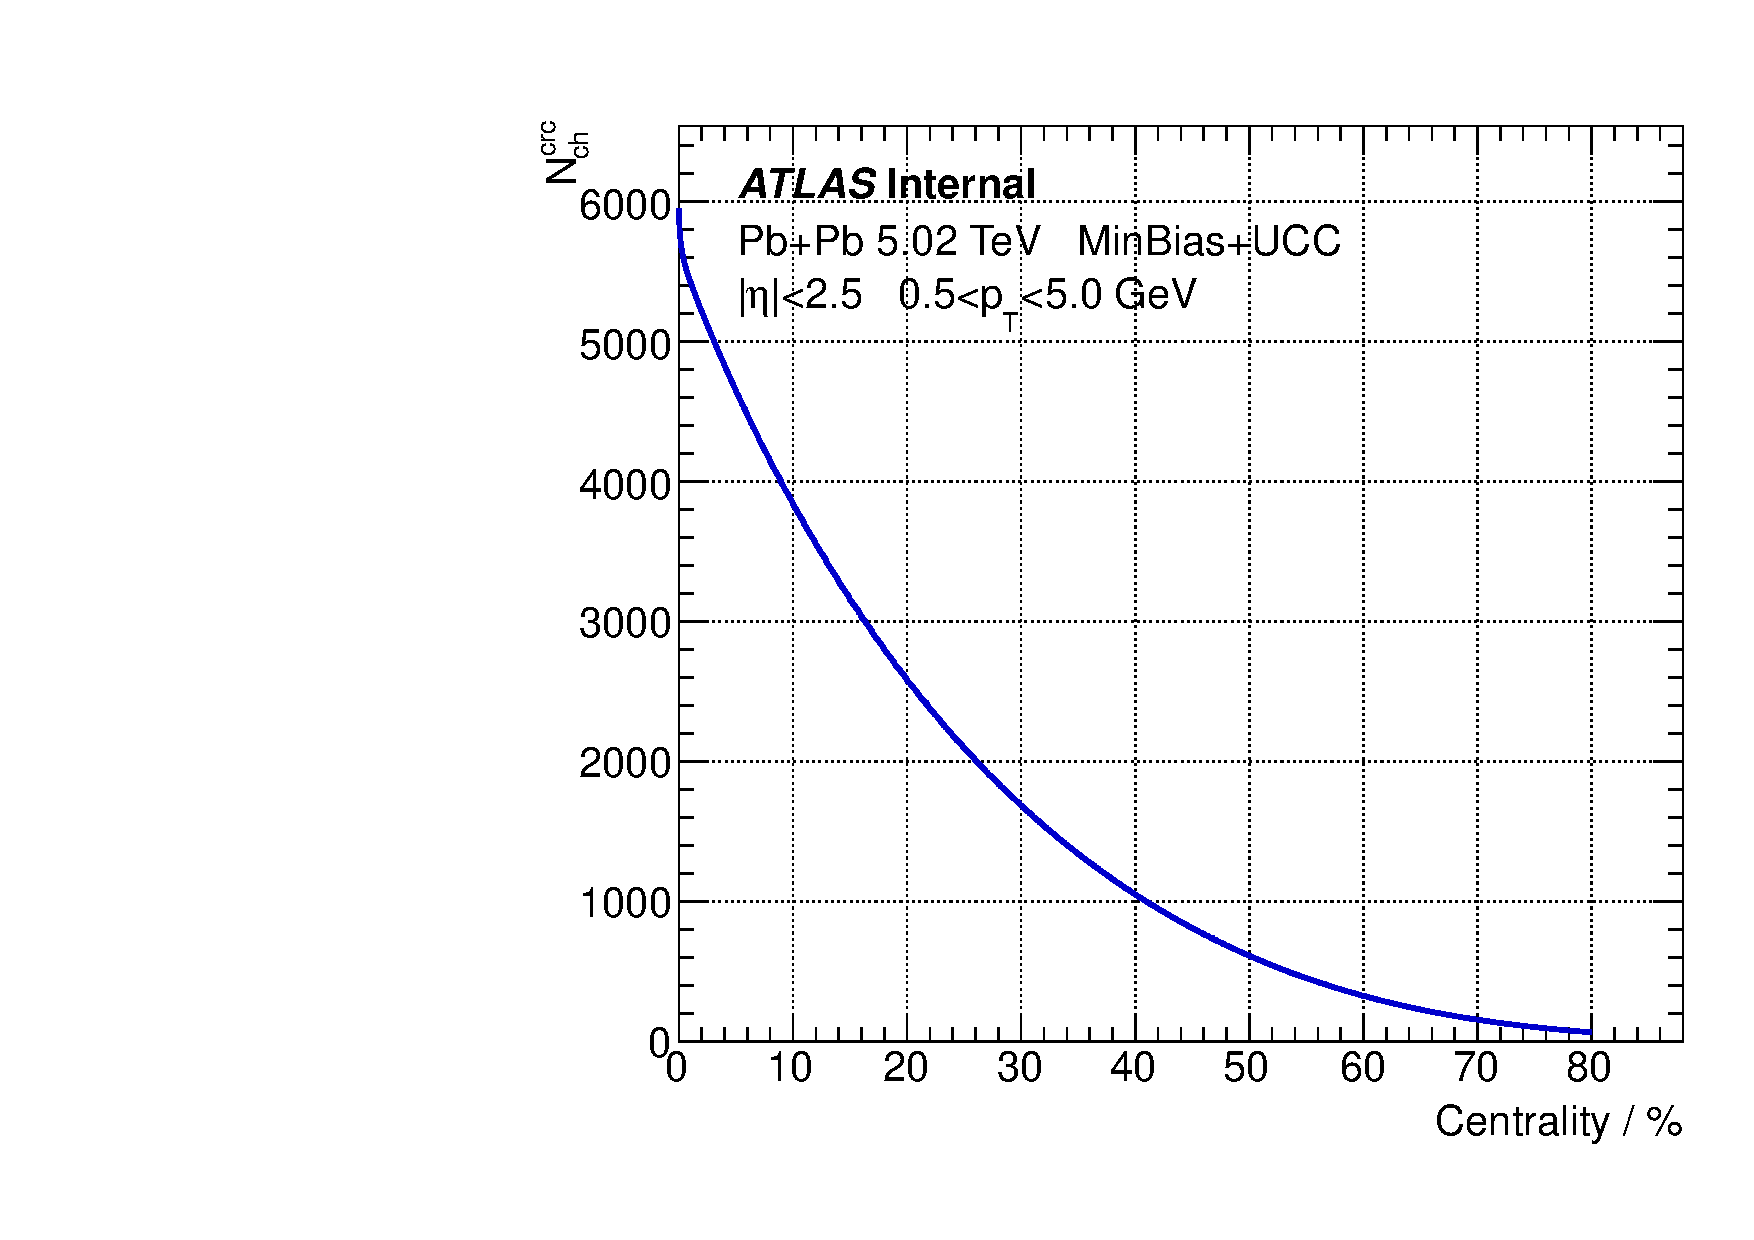
\includegraphics[width=.32\linewidth]{figs/sec_ana/cvtMap_cent_NchCrc.pdf}
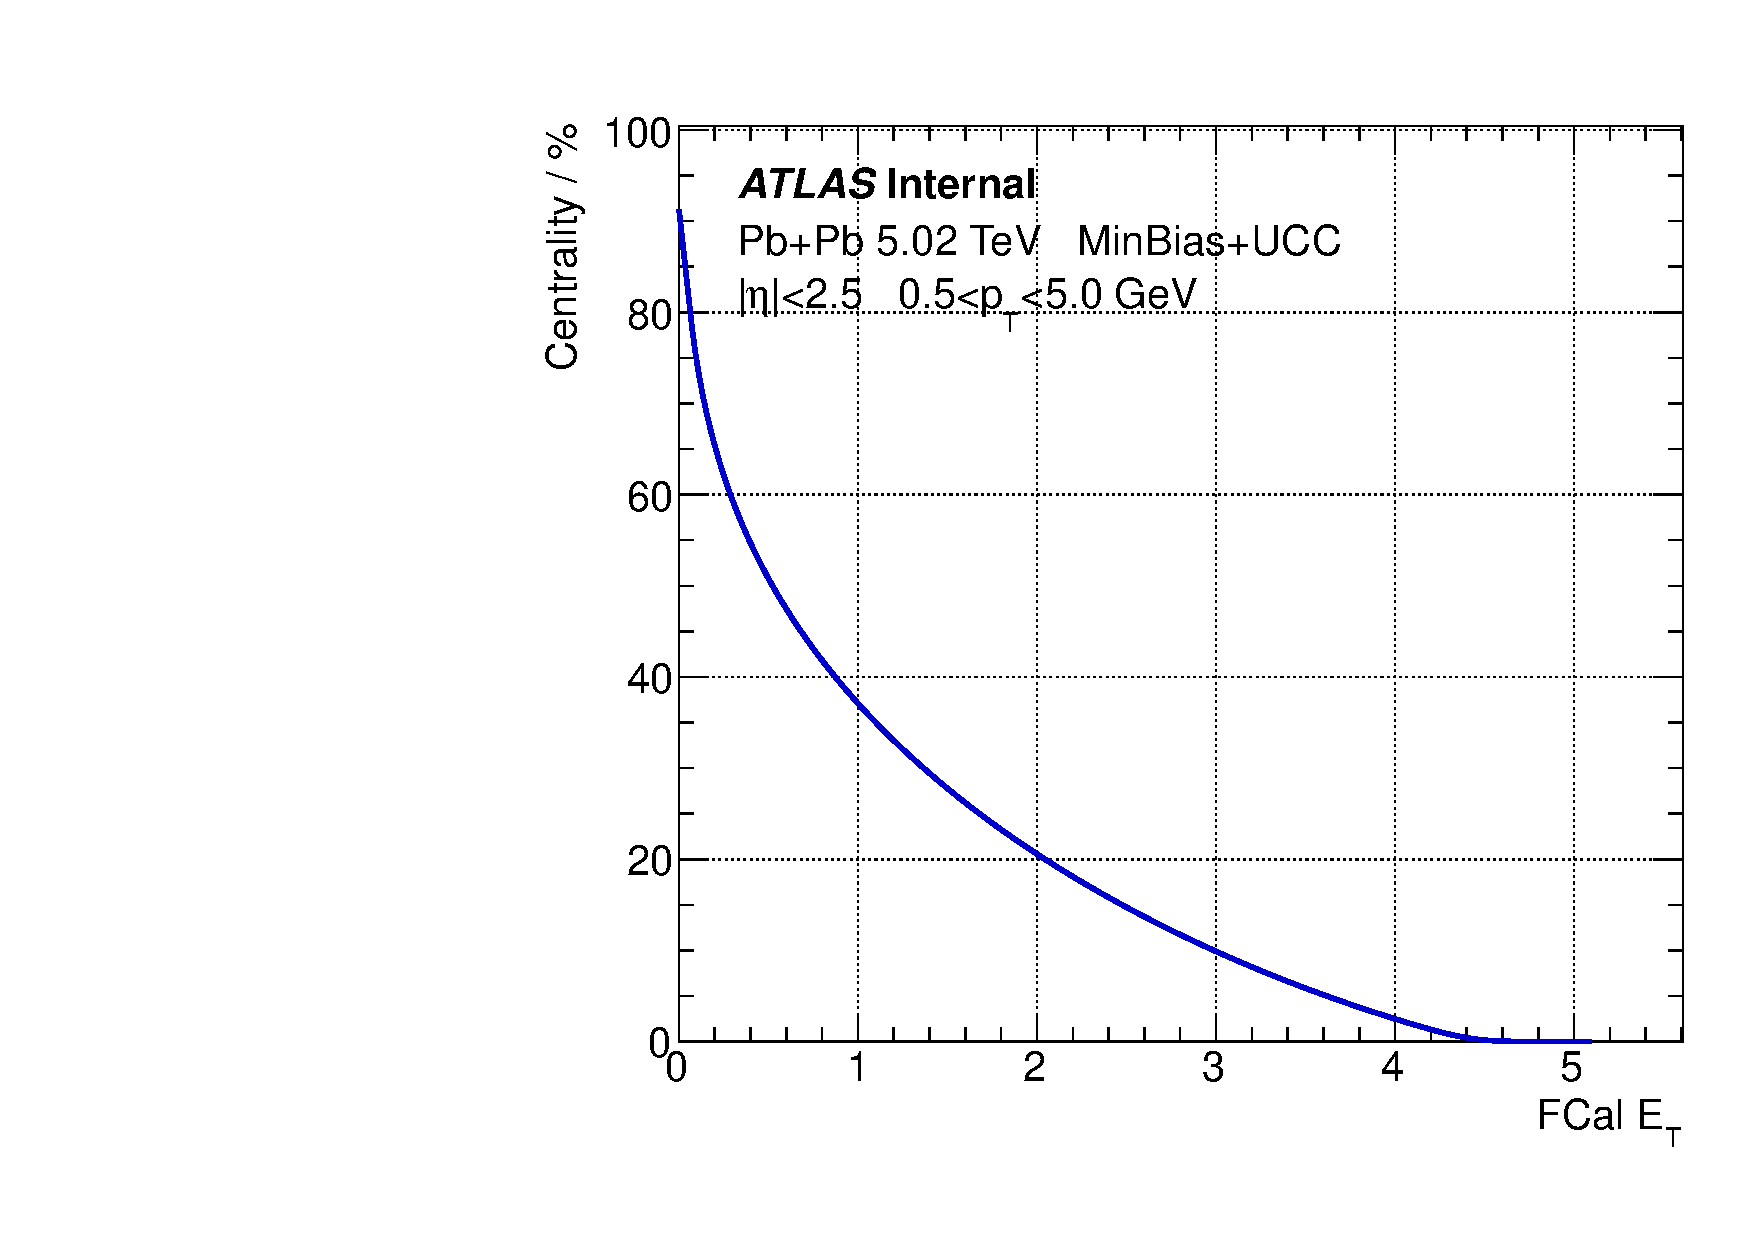
\includegraphics[width=.32\linewidth]{figs/sec_ana/cvtMap_fcal_cent.pdf}
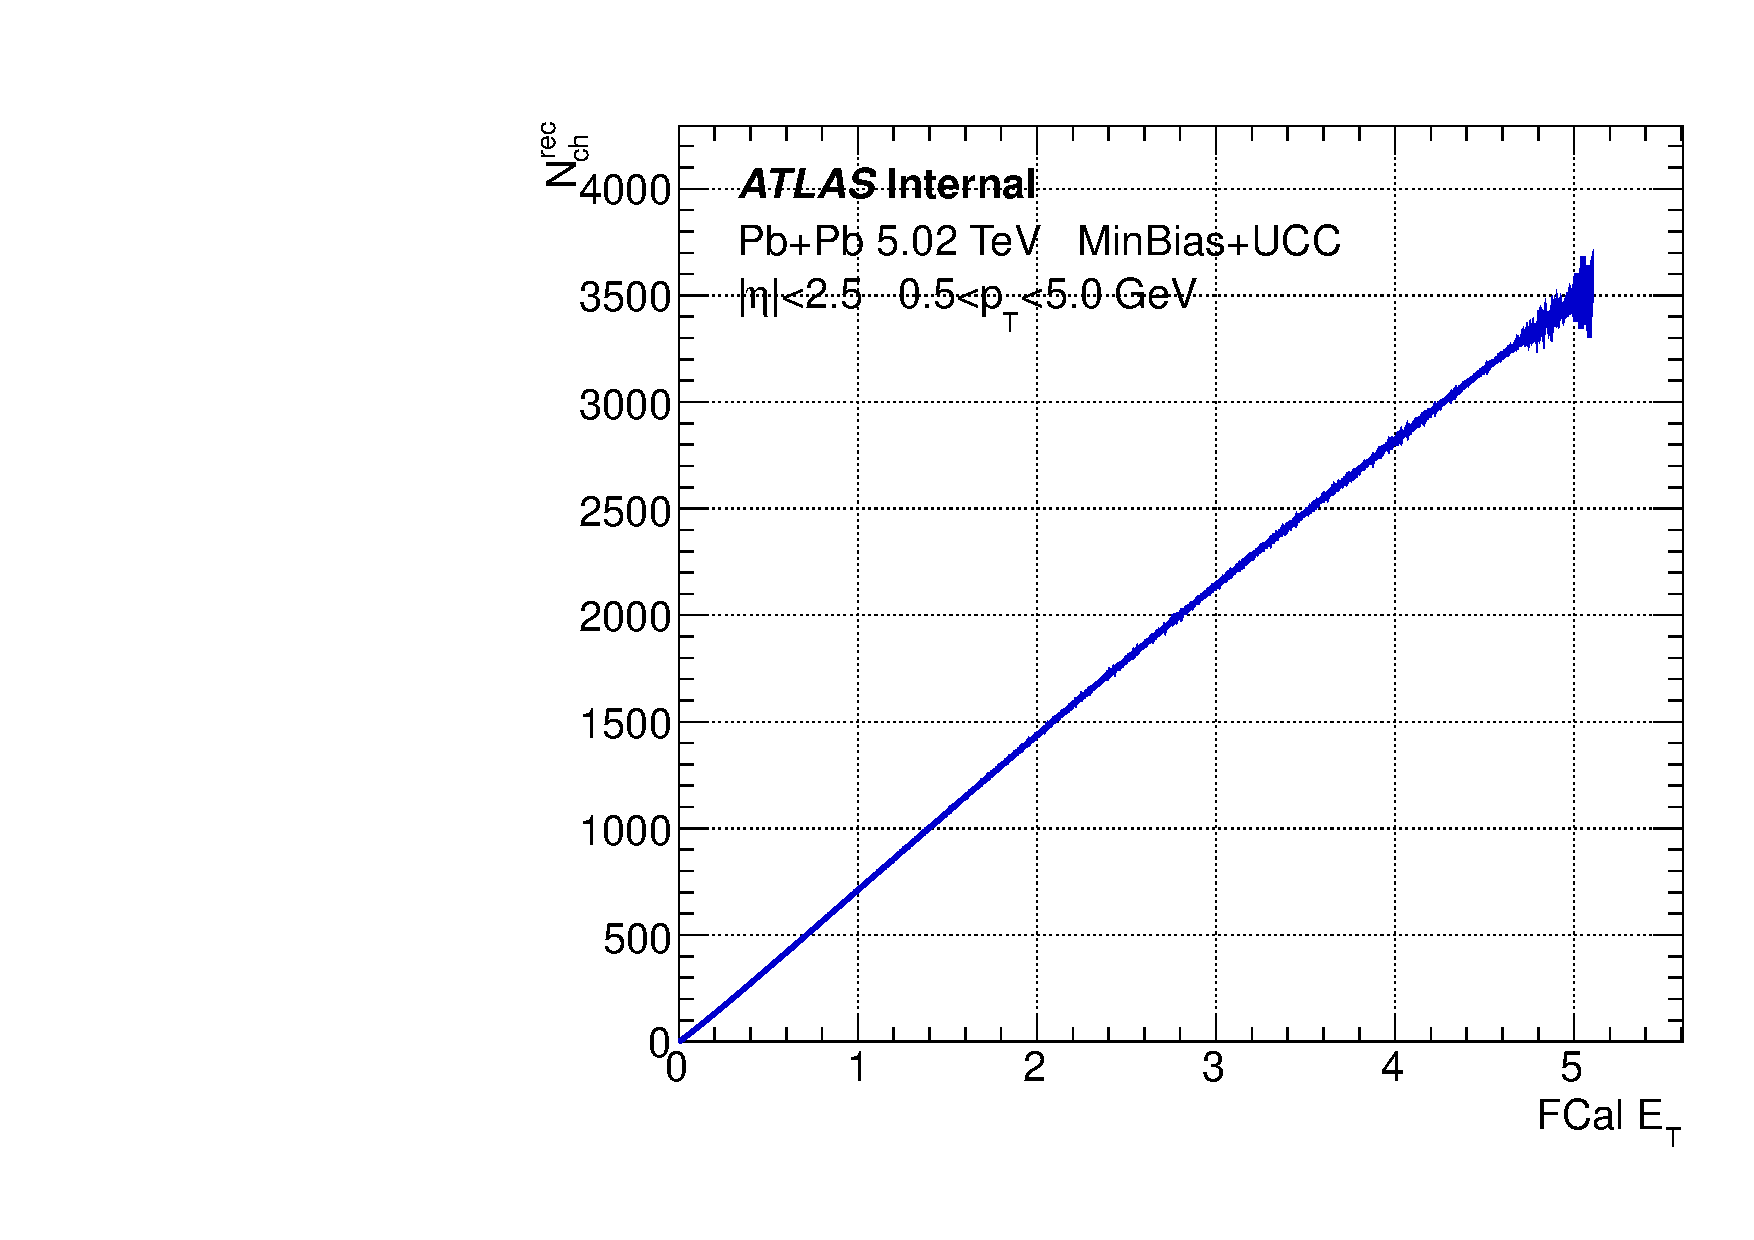
\includegraphics[width=.32\linewidth]{figs/sec_ana/cvtMap_fcal_NchRec.pdf}
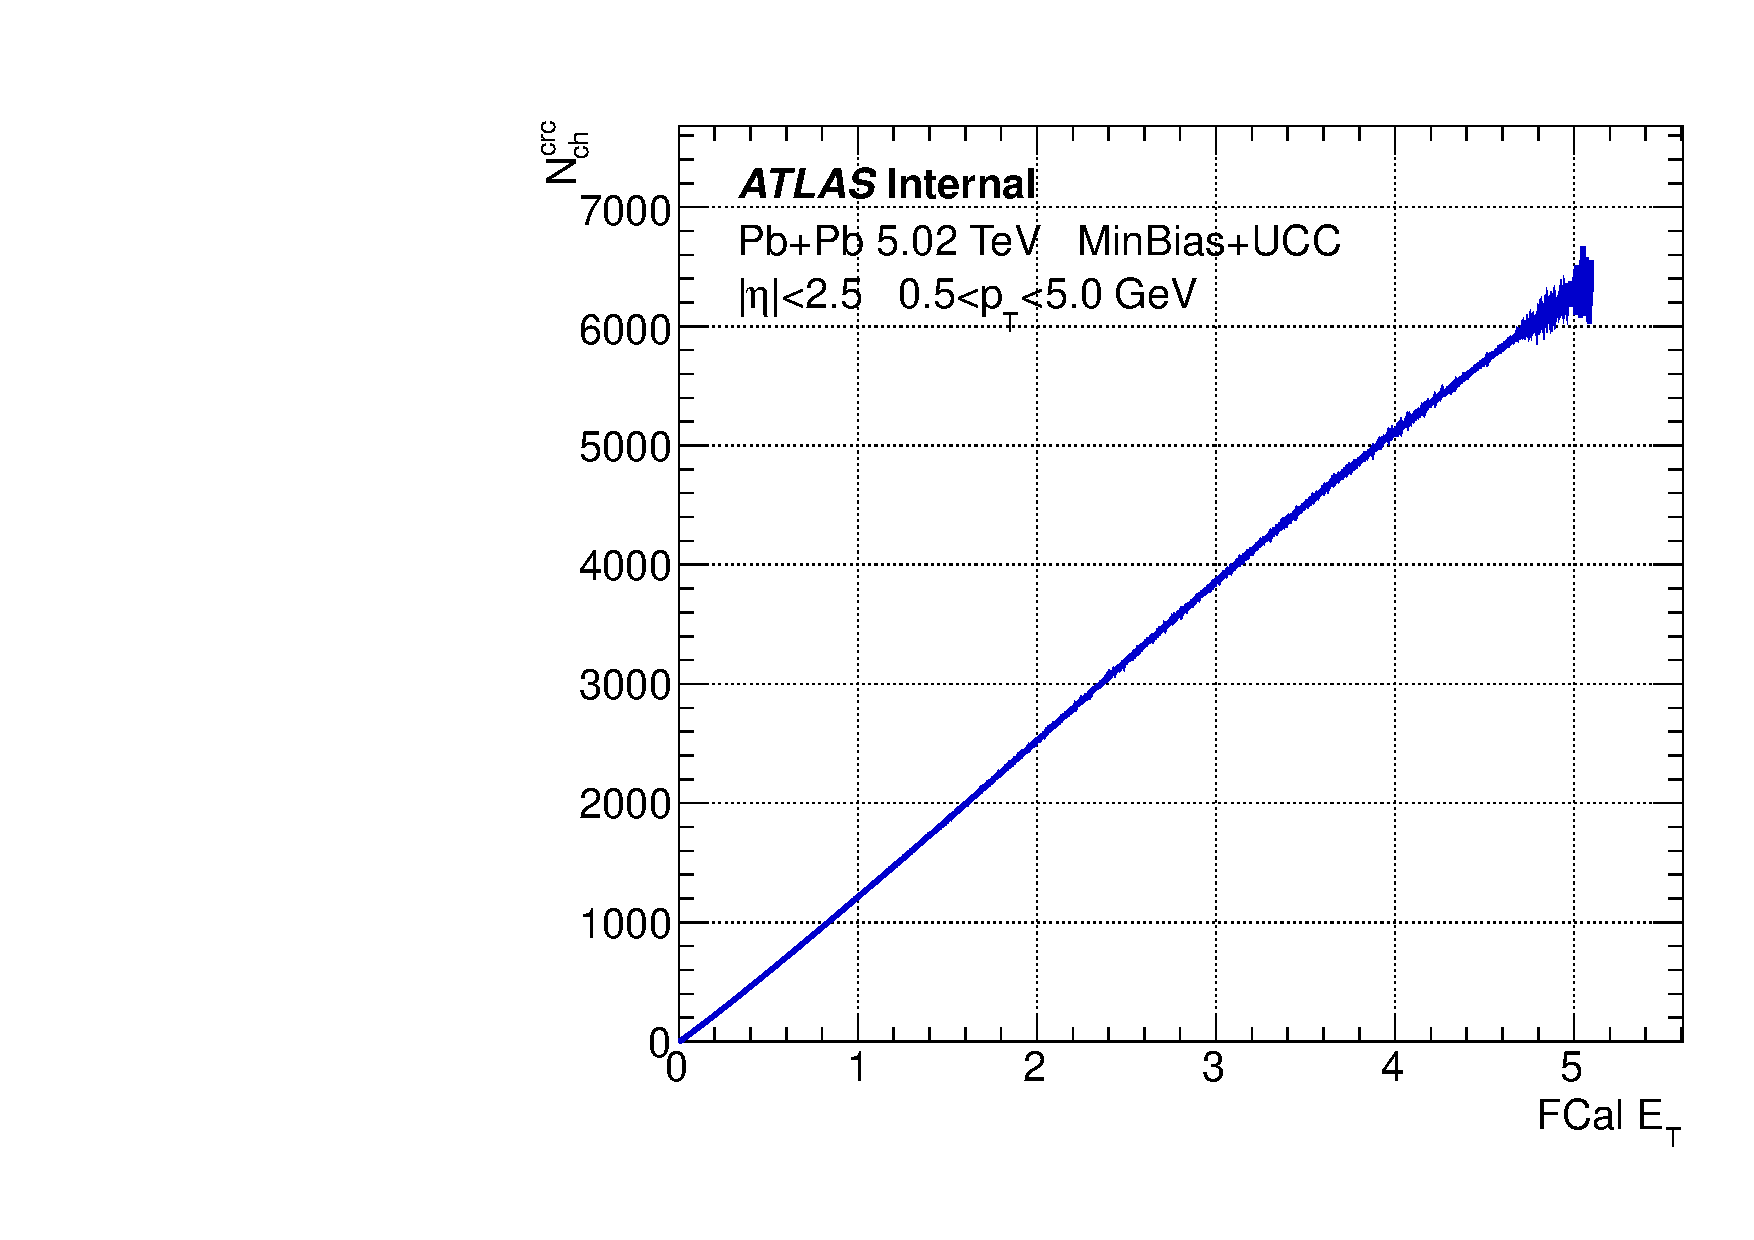
\includegraphics[width=.32\linewidth]{figs/sec_ana/cvtMap_fcal_NchCrc.pdf}
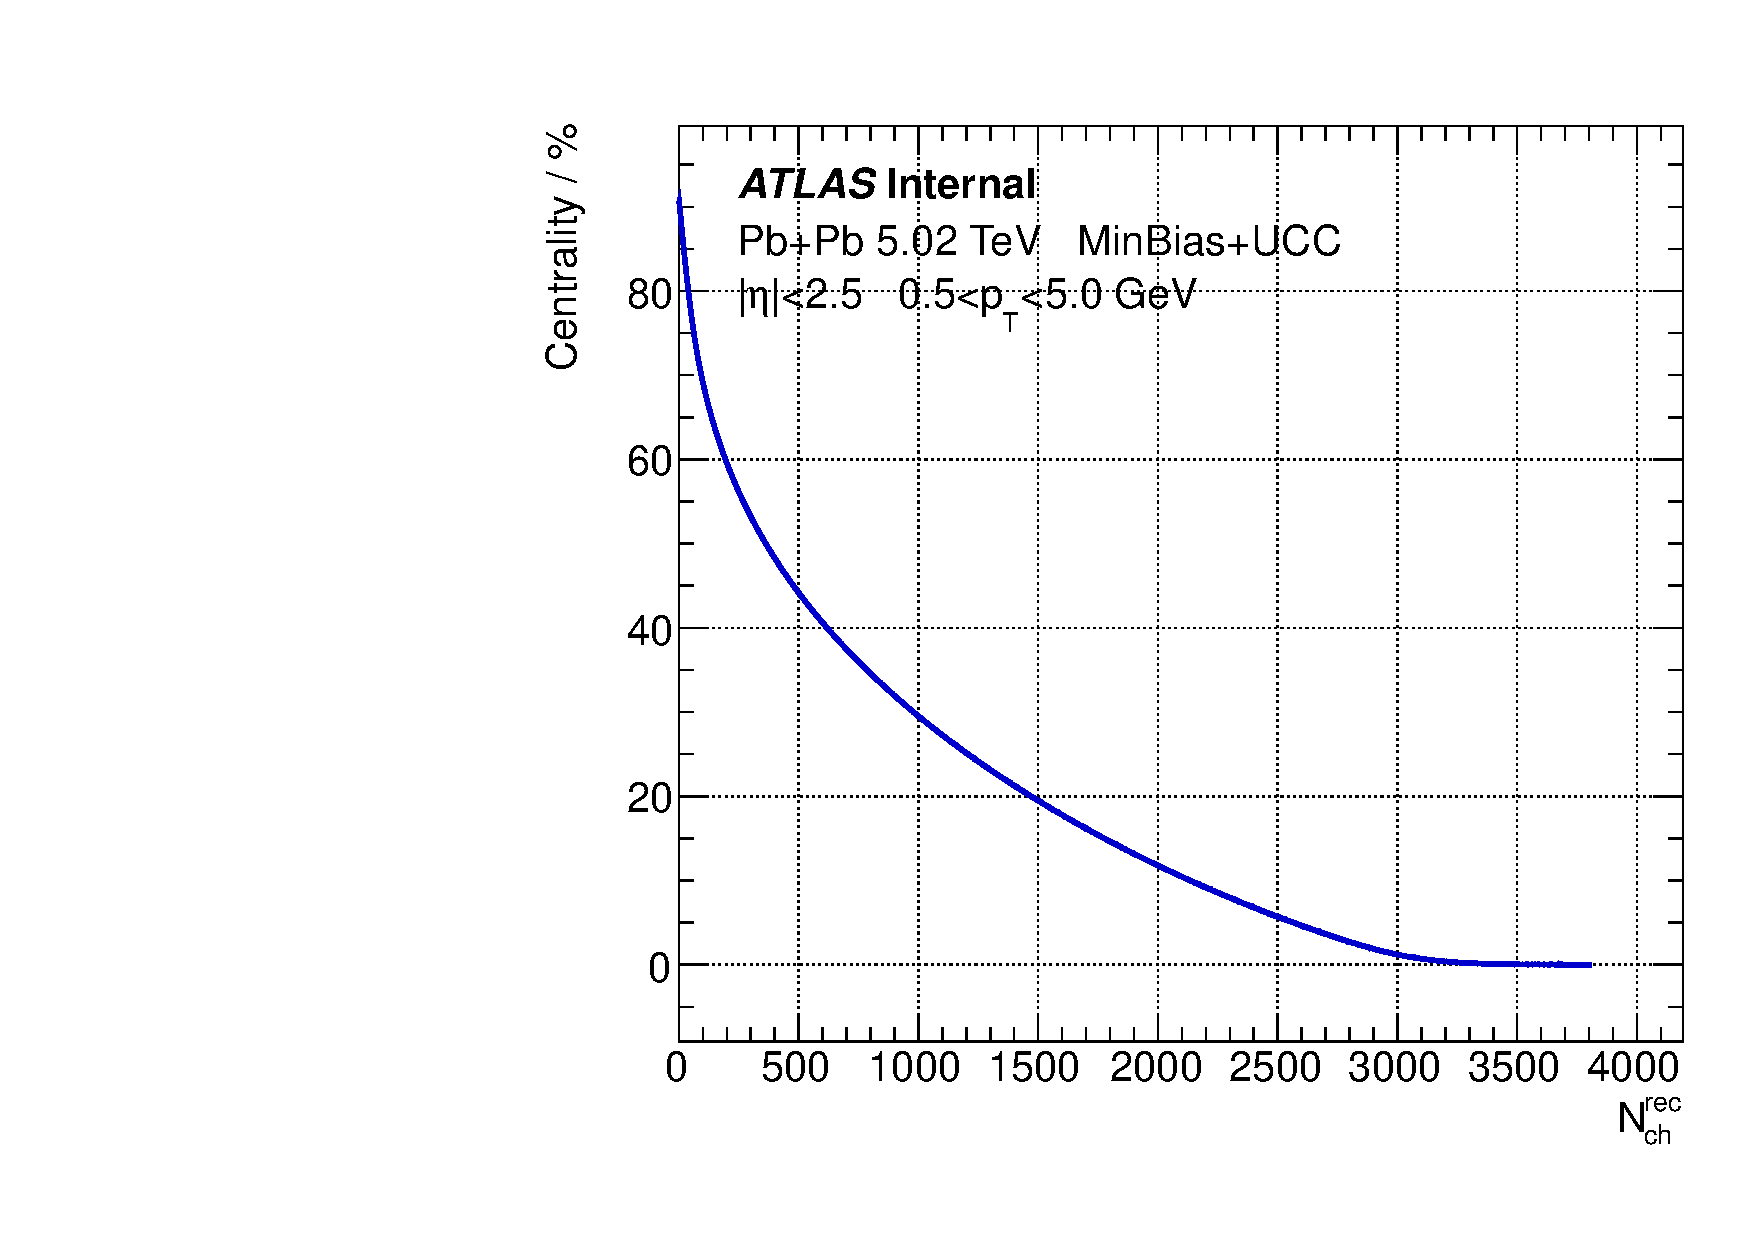
\includegraphics[width=.32\linewidth]{figs/sec_ana/cvtMap_NchRec_cent.pdf}
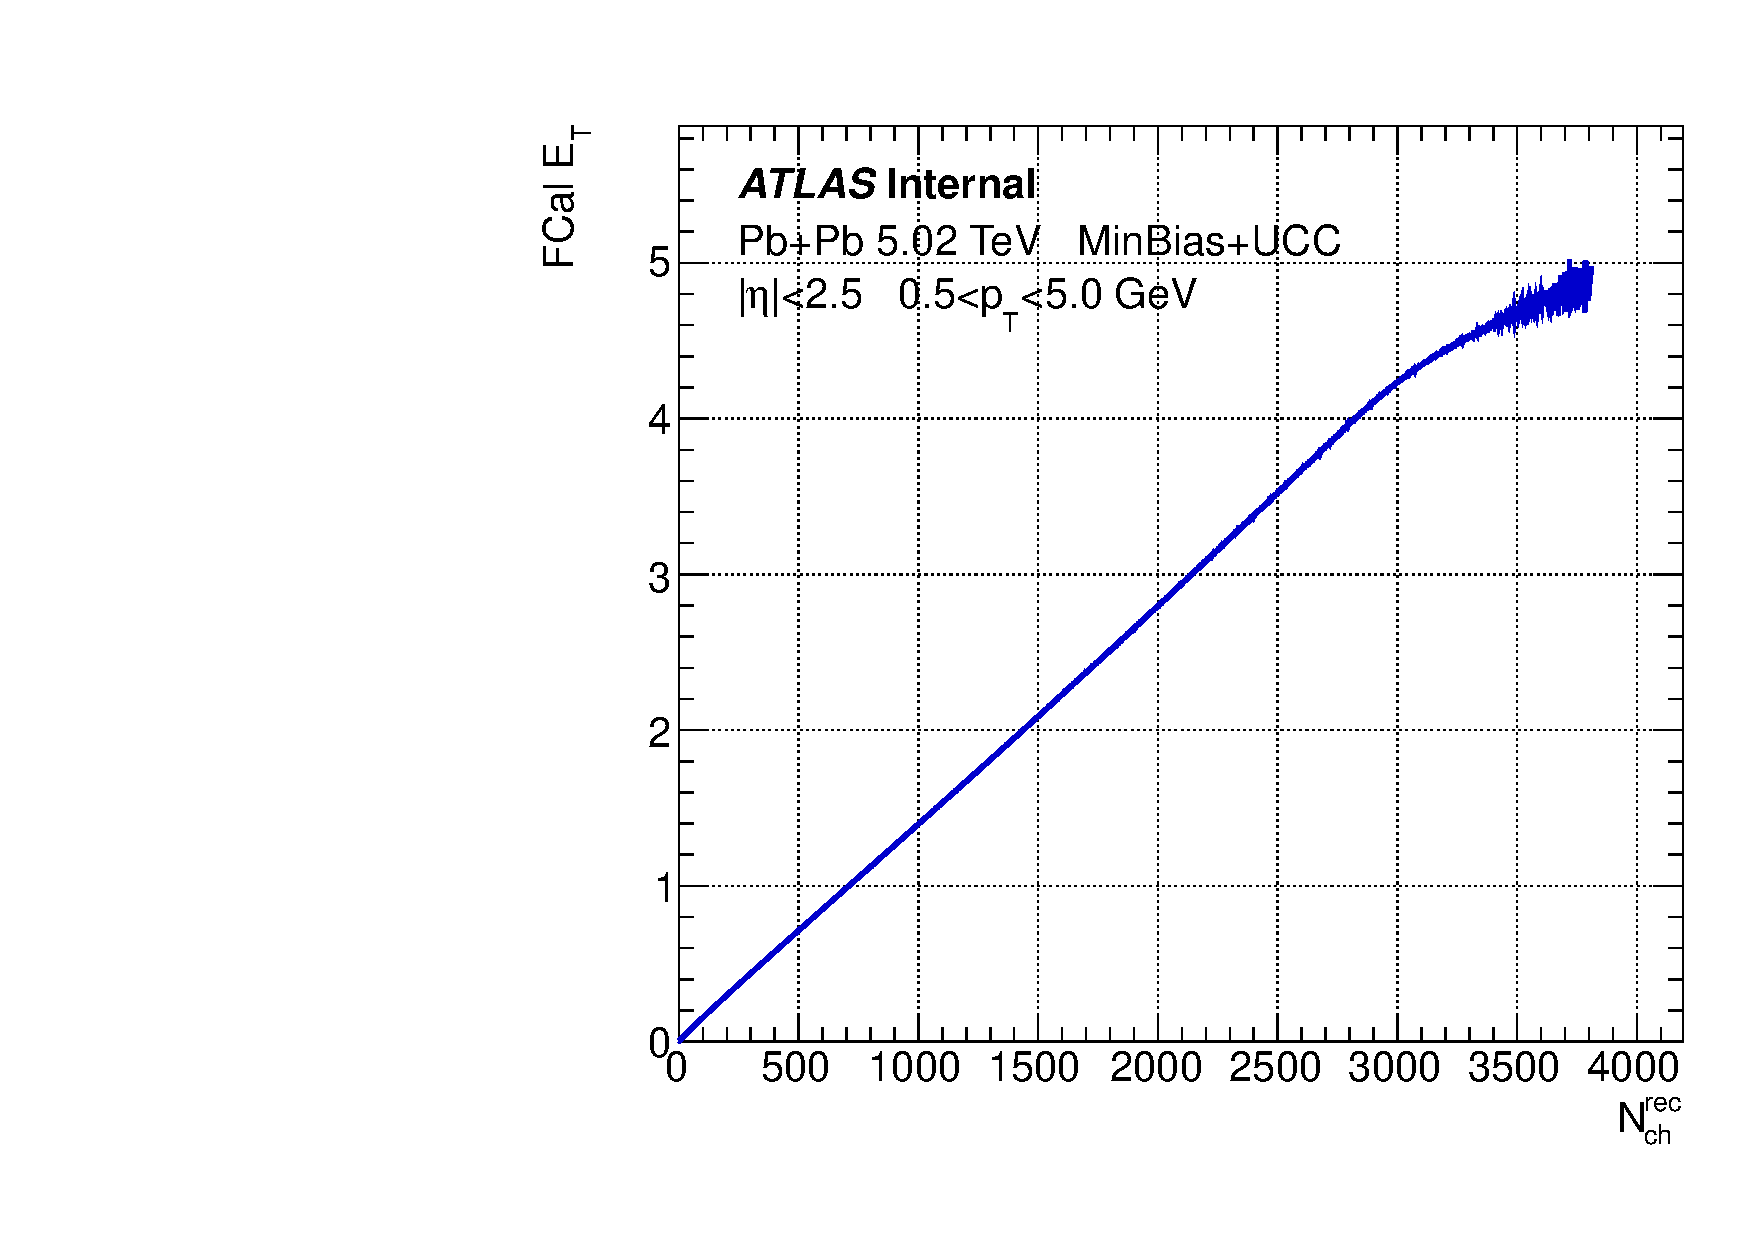
\includegraphics[width=.32\linewidth]{figs/sec_ana/cvtMap_NchRec_fcal.pdf}
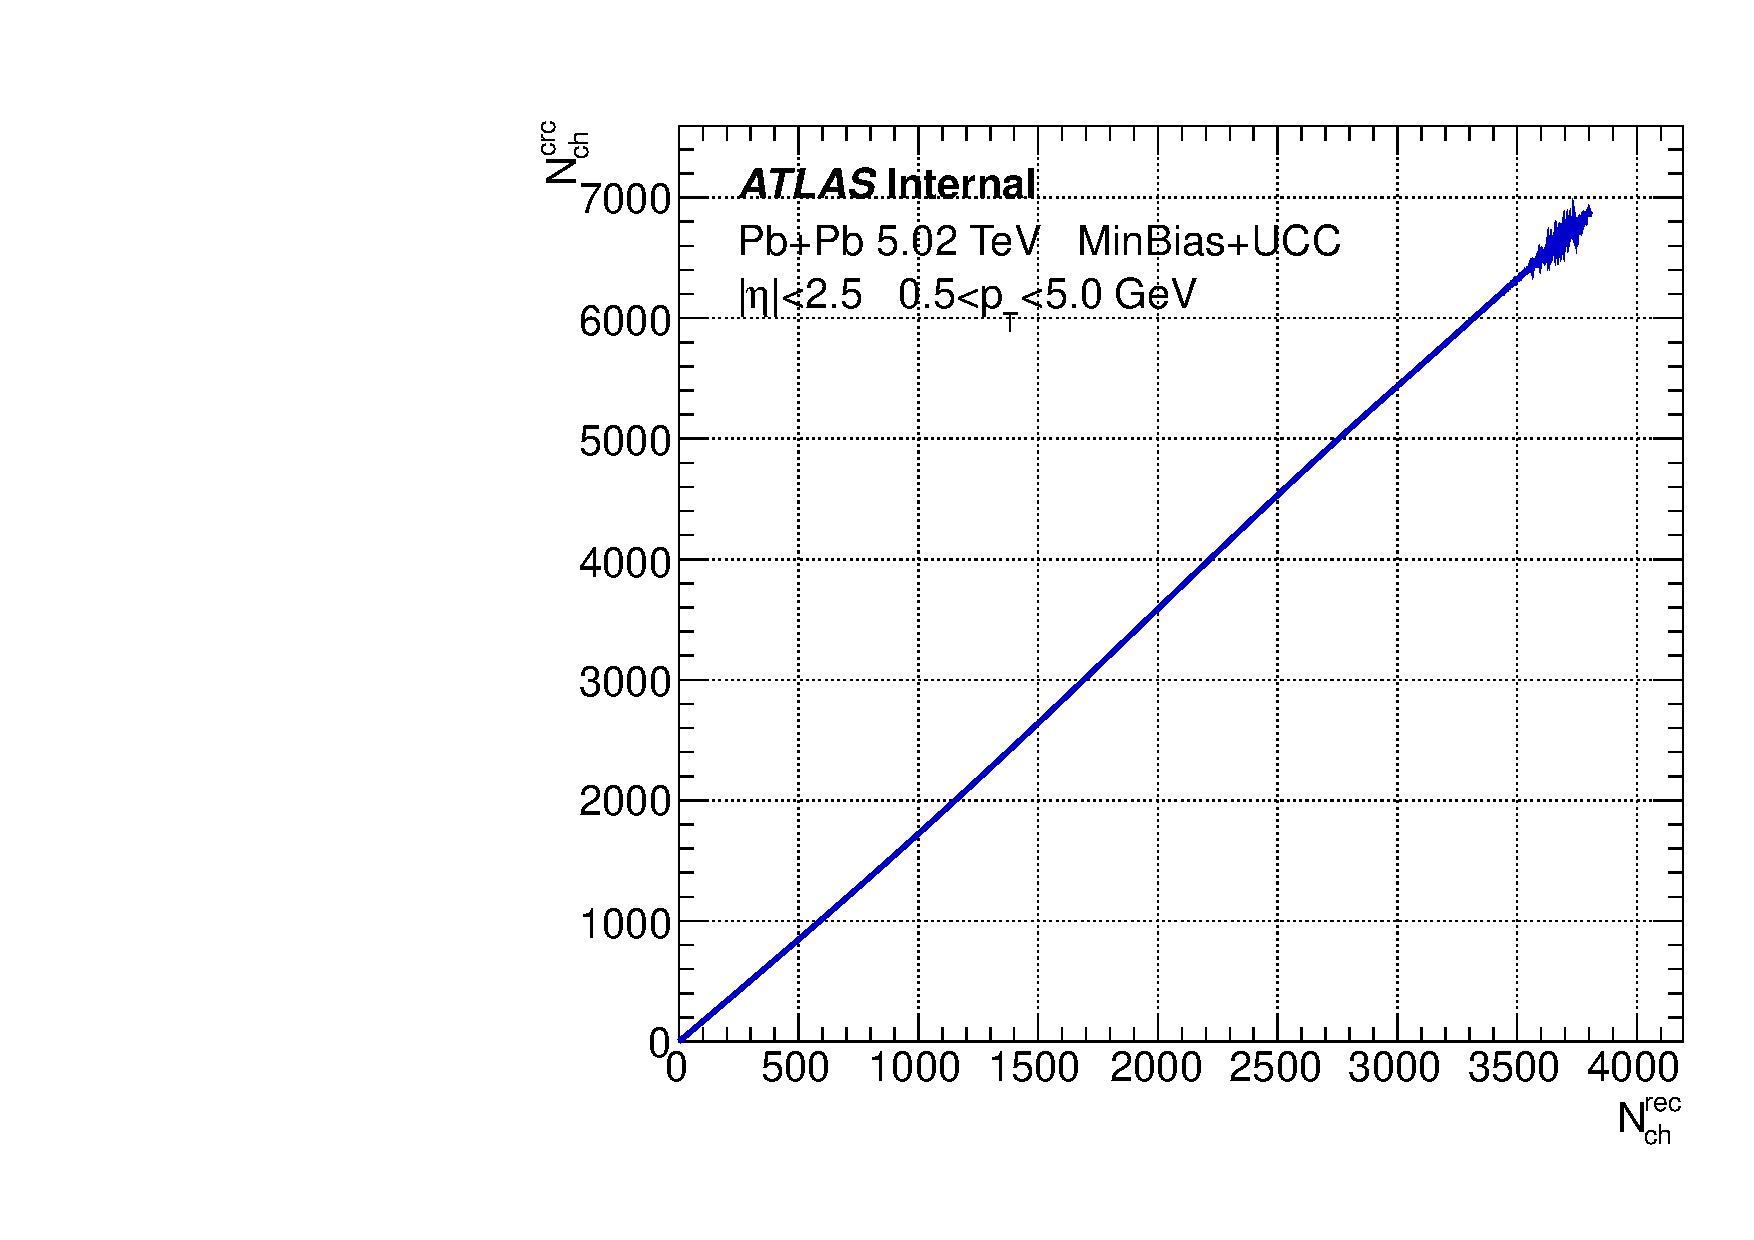
\includegraphics[width=.32\linewidth]{figs/sec_ana/cvtMap_NchRec_NchCrc.pdf}
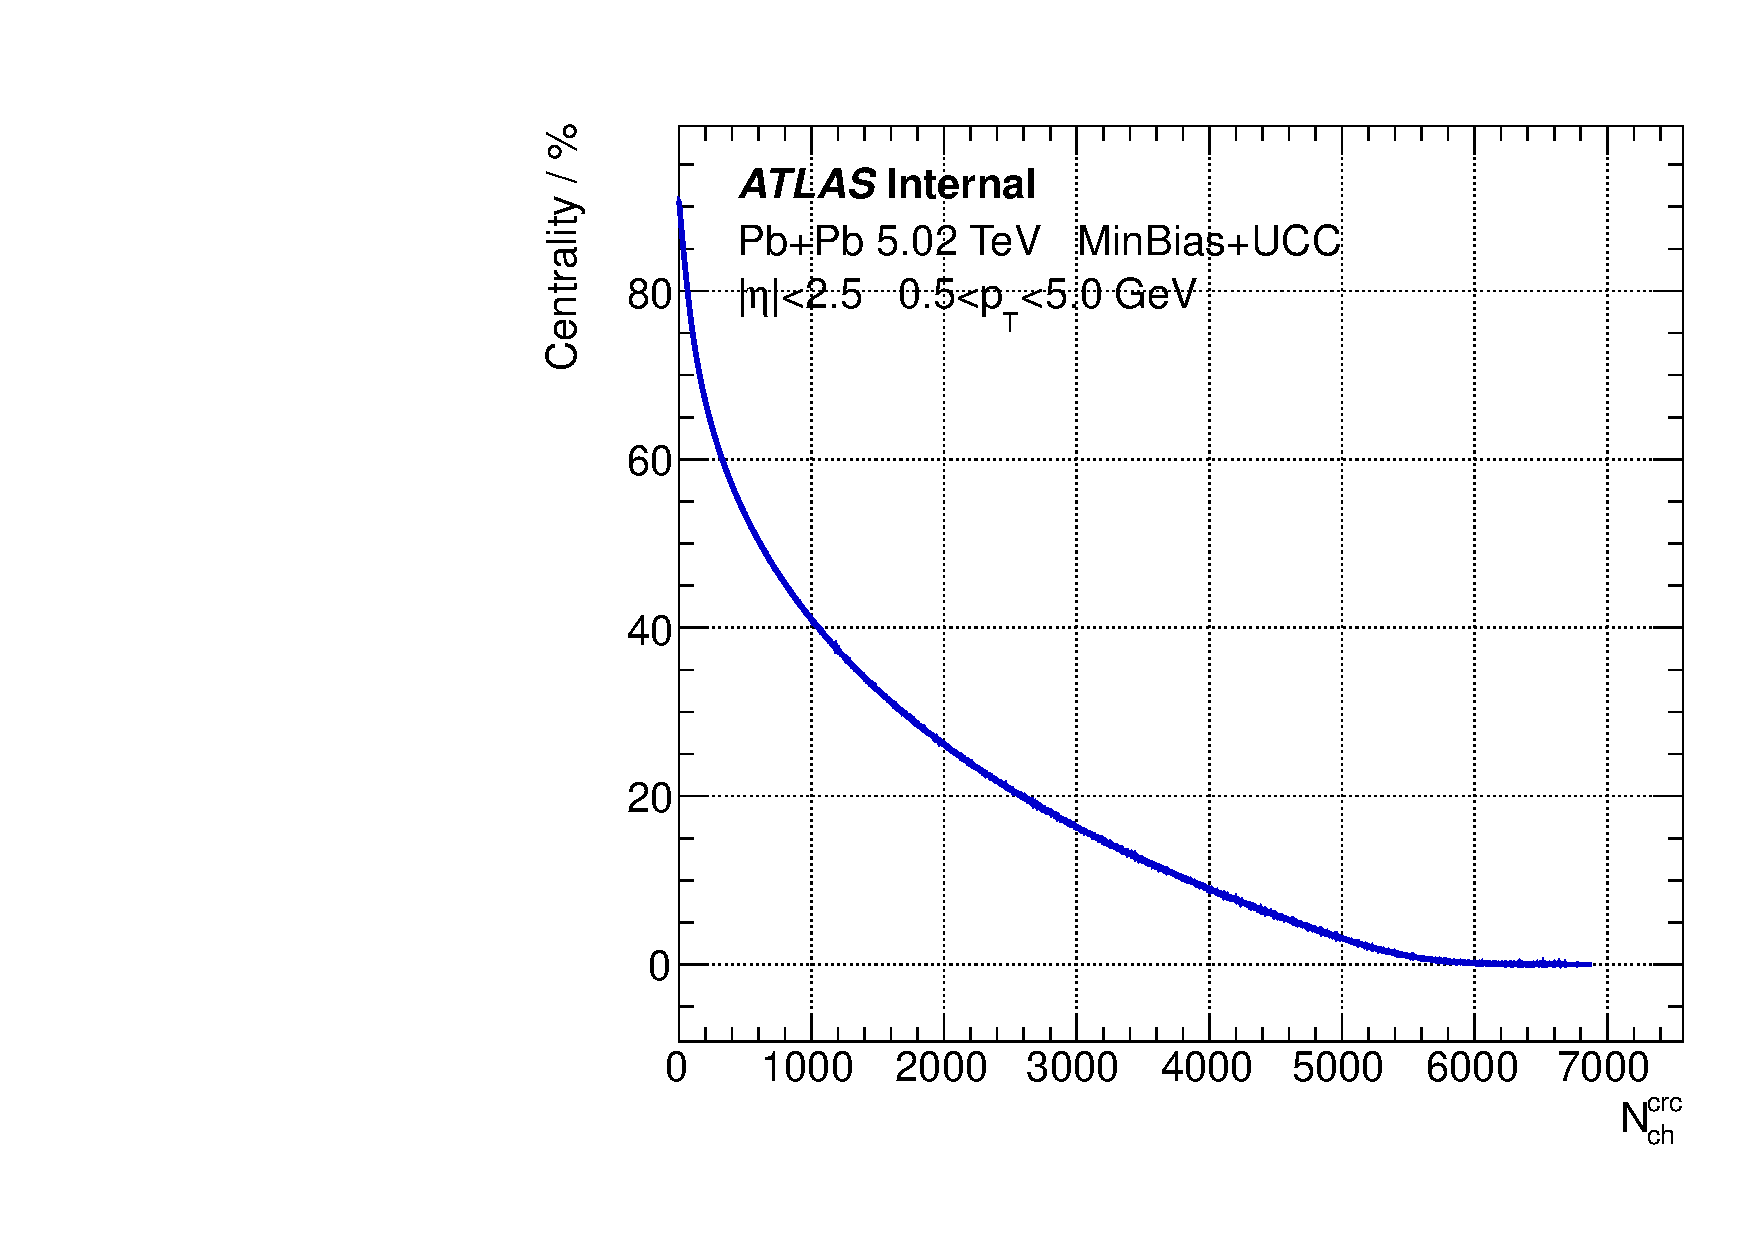
\includegraphics[width=.32\linewidth]{figs/sec_ana/cvtMap_NchCrc_cent.pdf}
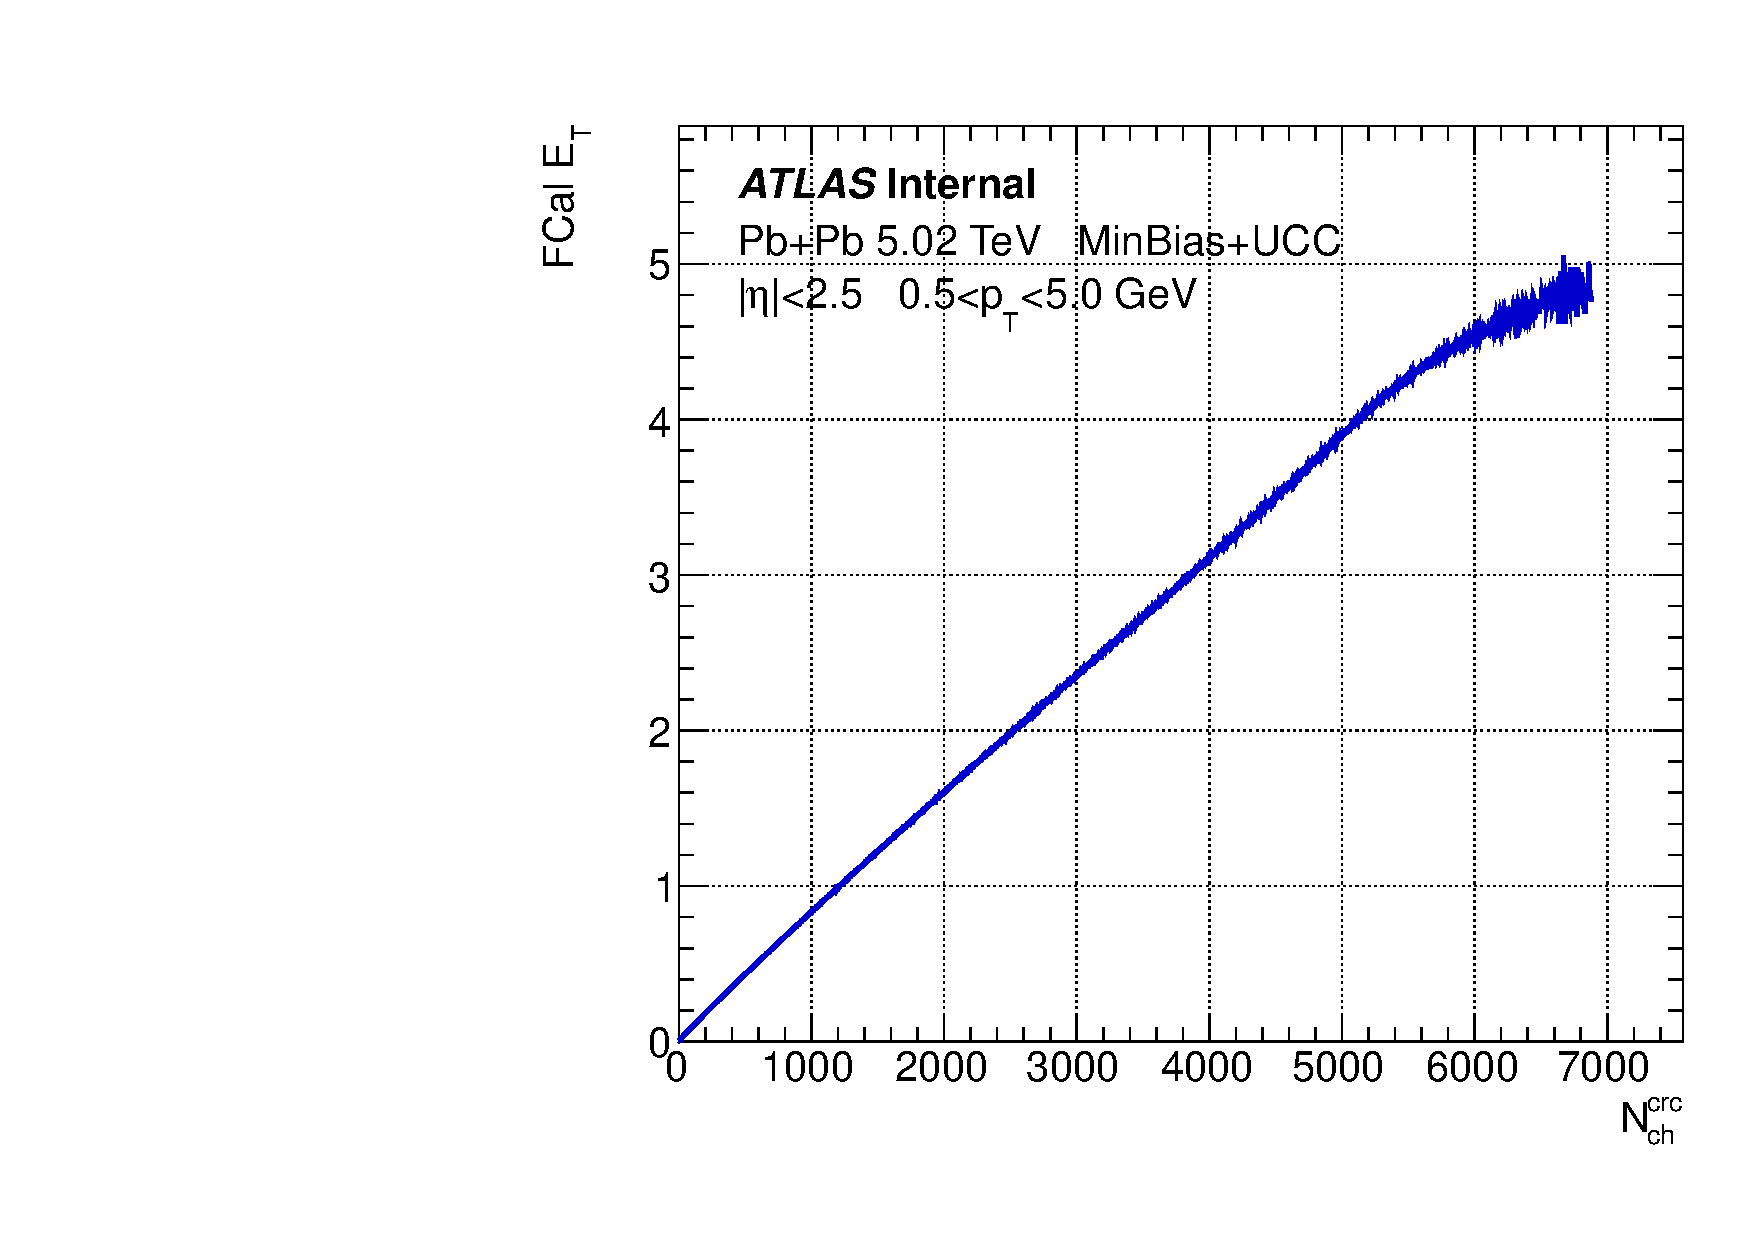
\includegraphics[width=.32\linewidth]{figs/sec_ana/cvtMap_NchCrc_fcal.pdf}
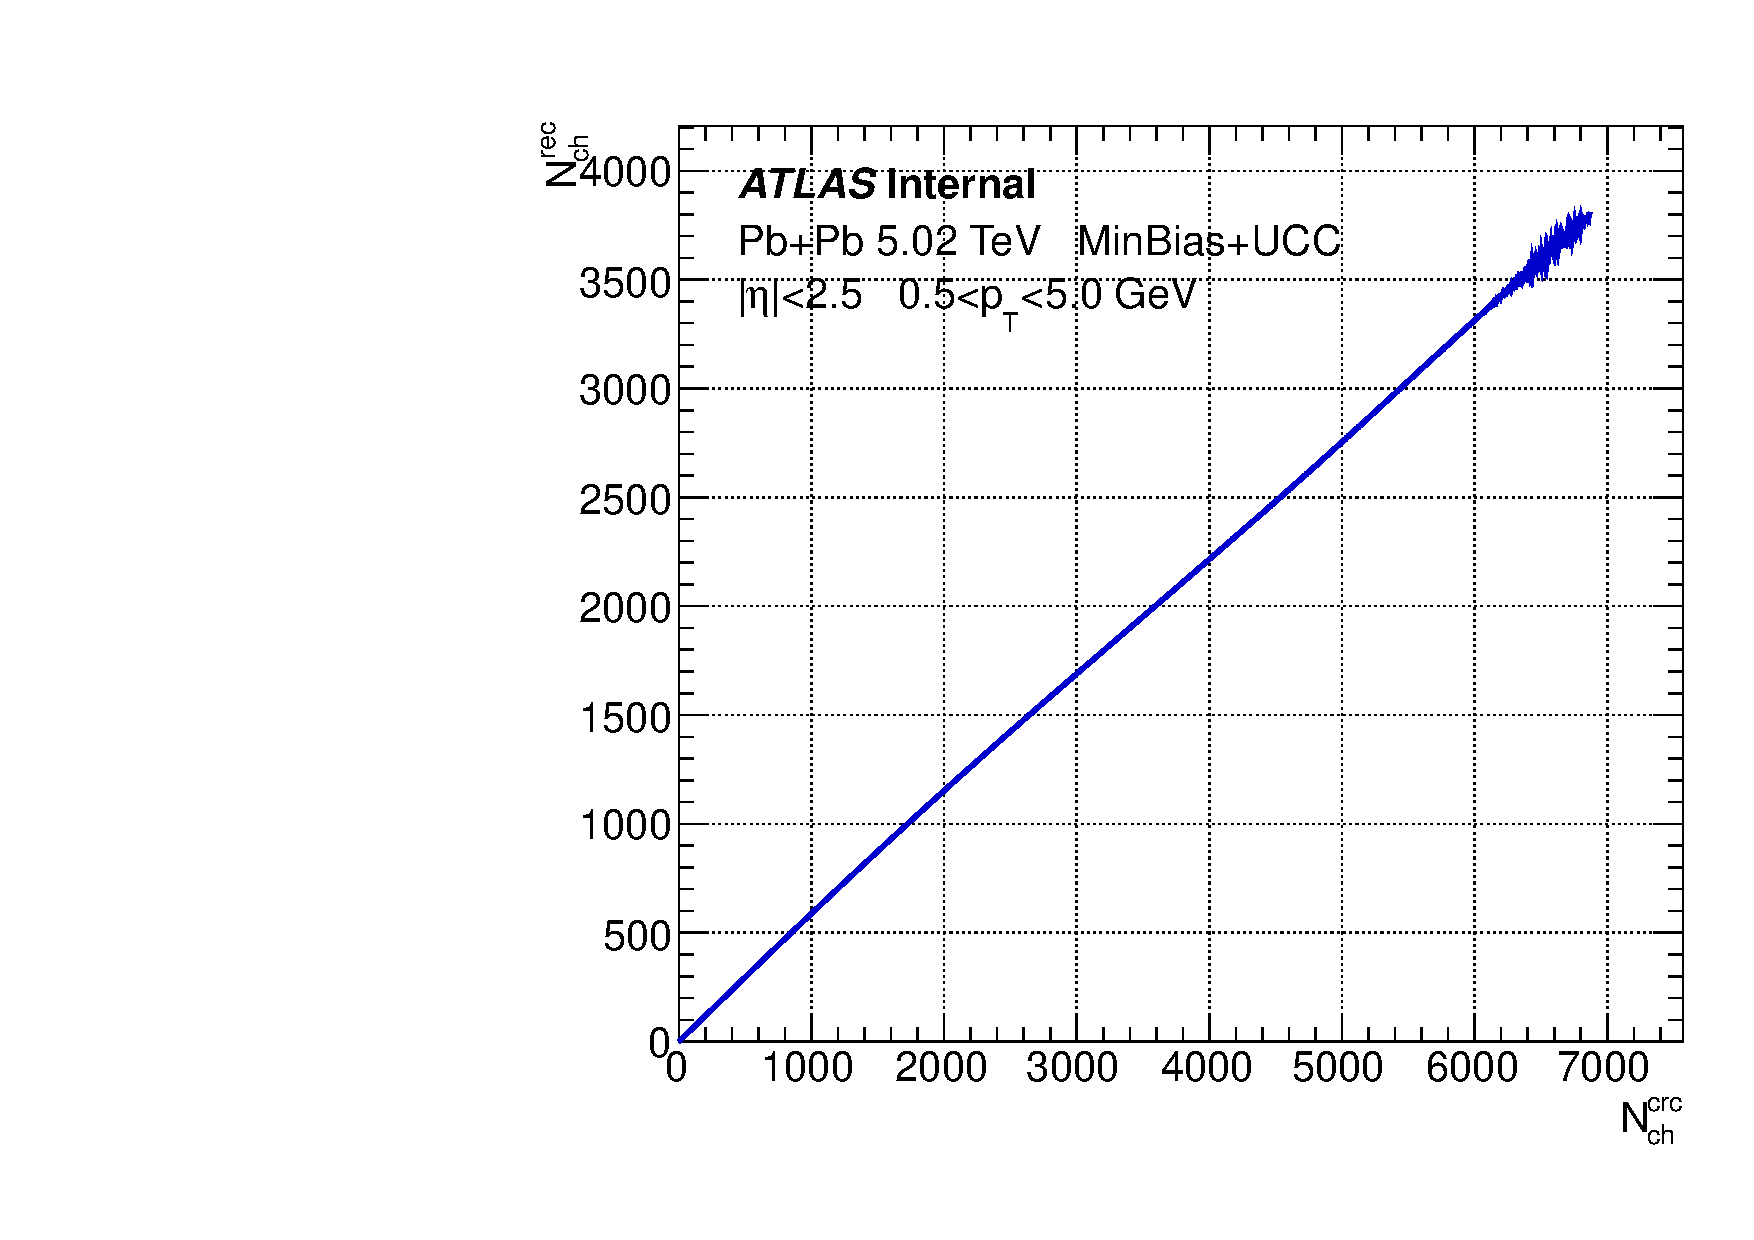
\includegraphics[width=.32\linewidth]{figs/sec_ana/cvtMap_NchCrc_NchRec.pdf}
\caption{Conversion maps among centrality, FCal sum $E_{T}$, reconstructed tracks $N_{ch}^{rec}$ and tracking efficiency corrected reconstructed tracks $N_{ch}^{crc}$. The Y-axis shows the mean value calculated in the event class defined by X-axis.}
\label{fig:ana_cvt}
\end{figure}
The conversion maps among centrality, FCal $E_\text{T}$, number of reconstructed tracks $N_{ch}^{rec}$ and number of corrected reconstructed tracks $N_{ch}^{crc}$ are listed in Fig.~\ref{fig:ana_cvt}, where the Y-axis indicates the mean value calculated in the event class defined by the X-axis. When necessary, these maps are used to convert results with different event class definitions into the same X-axis.



\subsection{Mixed events}
To correct the detector effects, we weighted the tracks by the tracking efficiency and fraction of fake tracks obtained from Monte-Carlo plus the detector simulation. In additional, $w_\phi$ obtained from flattening procedure is applied as the event weight to further suppress the detector effects in the transverse plane. To estimate the residual detector effects, a mixed event technique can be implemented. In this section, we will discuss why mixed event work and how to implement it.

Compared with the physics signal, the major feature of detector effect is that it does not fluctuate from event to event. In other words, detector effects are correlated across "similar" events that are neighbouring in time. By "similar", it requires those events have the similar centrality and $z$ position of primary vertex $z_{vtx}$. On the other hand, the physics signal, like flow, are correlated within a single event, but uncorrelated between different events. Using these features, the mixed event can be reconstructed by measuring the correlation among different events.

In the following we will take the calculation of $c_{n}\{4\}$ as one example to show how to calculate the corresponding mixed events. The definition of 2- and 4-particle correlation in mixed events is written as:
\begin{equation}
\begin{split}
corr_{n}^{bk}\{2\}&\equiv \lr{e^{i\text{n}(\phi_i-\phi_j)}} \\
corr_{n}^{bk}\{4\}&\equiv \lr{e^{i\text{n}(\phi_i+\phi_j-\phi_k-\phi_l)}}
\end{split}
\end{equation}
where $bk$ in the superscript is used to separate the mixed event (background) from the original signal (foreground). The definition seems to be identical to the $corr_{n}\{2k\}$ in a single event, however, now $i, j, k$ and $l$ are particles coming from 4 different events that are neighbouring in time. Note that there are 3 equivalent permutation of $i, j, k$ and $l$: $(\phi_i+\phi_j-\phi_k-\phi_l)$, $(\phi_i+\phi_k-\phi_j-\phi_l)$ and $(\phi_i+\phi_l-\phi_j-\phi_k)$ and they should all be included when calculating the background.

In the definition of $corr_{n}^{bk}\{2\}$ and $corr_{n}^{bk}\{4\}$, since particle can never be correlated with itself, all duplicates are gone. Thus the Q-cumulant formula are much simpler compared with the calculation of foreground:
\begin{equation}
\begin{split}
corr_n^{bk}\{2\}&=\frac{\mathcal{R}\textit{e}(\pmb{Q}_{n,1}^{i}\pmb{Q}_{n,1}^{j*})}{S_{1,1}^i S_{1,1}^j} \\
corr_n^{bk}\{4\}&=\frac{\mathcal{R}\textit{e}(\pmb{Q}_{n,1}^{i}\pmb{Q}_{n,1}^{j}\pmb{Q}_{n,1}^{k*}\pmb{Q}_{n,1}^{l*})}{S_{1,1}^i S_{1,1}^j S_{1,1}^k S_{1,1}^l}
\end{split}
\end{equation}
where $i, j, k$ and $l$ denotes 4 different events.

Then followed the same procedure, the $corr_n^{bk}\{2k\}$ are averaged in each event class to get $\lr{corr_n^{bk}\{2k\}}$. The 4-particle cumulant from background can also be defined in the same way:
\begin{equation}
c_{n}^{bk}\{4\}=\lr{corr_n^{bk}\{4\}}-2\lr{corr_n^{bk}\{2\}}^2
\end{equation}
where the event class is defined by the first event $i$ in the mixed events.

In the end, we subtract the cumulant calculated in mixed events from the foreground, to obtain the corrected cumulant:
\begin{equation}
c_{n}^{crt}\{4\}\equiv c_{n}\{4\}-c_{n}^{bk}\{4\}
\end{equation}
In the measurement section, without special mention, All cumulant results are using $c_{n}^{crt}\{2k\}$ as the default.



\subsection{Statistical uncertainty}
Cumulant analysis, especially for higher order cumulant, suffers from statistics, which makes it crucial to correctly calculated the statistical uncertainty. The errors can be directly calculated from the cumulant definition, by using appropriate error propagation. Take 4-particle standard cumulant as an example:
\begin{equation}
c_n\{4\}=\lr{corr_n\{4\}}-2\lr{corr_n\{2\}}^2
\end{equation}
where both $\lr{corr_n\{4\}}$ and $\lr{corr_n\{2\}}$ are averaged over many events, so the errors are calculated as:
\begin{equation}
\begin{split}
\delta^2(\lr{corr_n\{4\}})&\equiv \frac{\sum_i W^i\{4\}(corr_n^i\{4\}-\lr{corr_n\{4\}})^2}{\sum_i W^i\{4\}} \\
\delta^2(\lr{corr_n\{2\}})&\equiv \frac{\sum_i W^i\{2\}(corr_n^i\{2\}-\lr{corr_n\{2\}})^2}{\sum_i W^i\{2\}}
\end{split}
\end{equation}
However, since the weights $W^i\{4\}$ and $W^i\{2\}$ are not random, there is a correction factor to yield an unbiased estimator:
\begin{equation}
\begin{split}
\delta^2(\lr{corr_n\{4\}})&=(1-\frac{\sum_i (W^i\{4\})^2}{(\sum_i W^i\{4\})^2})\delta^2_\text{real}(\lr{corr_n\{4\}}) \\
\delta^2(\lr{corr_n\{2\}})&=(1-\frac{\sum_i (W^i\{2\})^2}{(\sum_i W^i\{2\})^2})\delta^2_\text{real}(\lr{corr_n\{2\}})
\end{split}
\end{equation}
where $\delta_\text{real}$ means the correct, unbiased statistical error estimator.

Note that both $\lr{corr_n\{4\}}$ and $\lr{corr_n\{2\}}$ measure the flow sign, so they are not independent variables. Thus the covariance needs to be considered while calculating the statistical errors for $c_n\{4\}$:
\begin{equation}
\delta^2(c_n\{4\})=\delta^2_\text{real}(\lr{corr_n\{4\}})+(4\lr{corr_n\{2\}})^2\delta^2_\text{real}(\lr{corr_n\{4\}})-8\lr{corr_n\{2\}}\text{cov}(\lr{corr_n\{4\}},\lr{corr_n\{2\}})
\end{equation}
where the covariance between $\lr{corr_n\{4\}}$ and $\lr{corr_n\{2\}}$ is denoted as $\text{cov}(\lr{corr_n\{4\}},\lr{corr_n\{2\}})$. As can be seen, it is quite cumbersome to calculate statistical error in this way: many histograms need to be saved in order to calculate the covariance. Furthermore, the formula are more complicated in subevent methods: up to 10 covariances will show up in the formula! Due to this reason, in this analysis, sub-sample technique is used to determine the statistical errors.

The sub-sample technique is a data-driven way to calculate the statistical errors, which is much easier to implement in the code. The first step is to randomly divide the whole data set into $N$ sub-samples ($N=20$ in this analysis). To guarantee that each sub-sample are not biased by run configuration like trigger setup and detector effects, in practice, we used random seeds to determine which sub-sample each event will fall into, which guarantees the dividing procedure to be random.

To demonstrate the random seed works, we have tested this produce on the 2015+2016 13 TeV low-$\mu$ $pp$ sample. The reason of choosing $pp$ is because the runs are throughout two years and run conditions as well as trigger setups are very different. The results are presented in Fig.~\ref{fig:ana_div}. Left plot shows the $N_{ch}$ distribution for the whole sample, where several "bumps" are from the high-multiplicity track (HMT) triggers. Right plot shows the relative difference of the statistics between sub-samples (indicated by different colors) and the mean ($5\%$ statistics of the whole sample), as a function of $N_{ch}$. As can be seen, the relative difference is within $1\%$ in the region where statistics are good. This demonstrates the dividing procedure produces randomly divided sub-samples.
\begin{figure}[H]
\centering
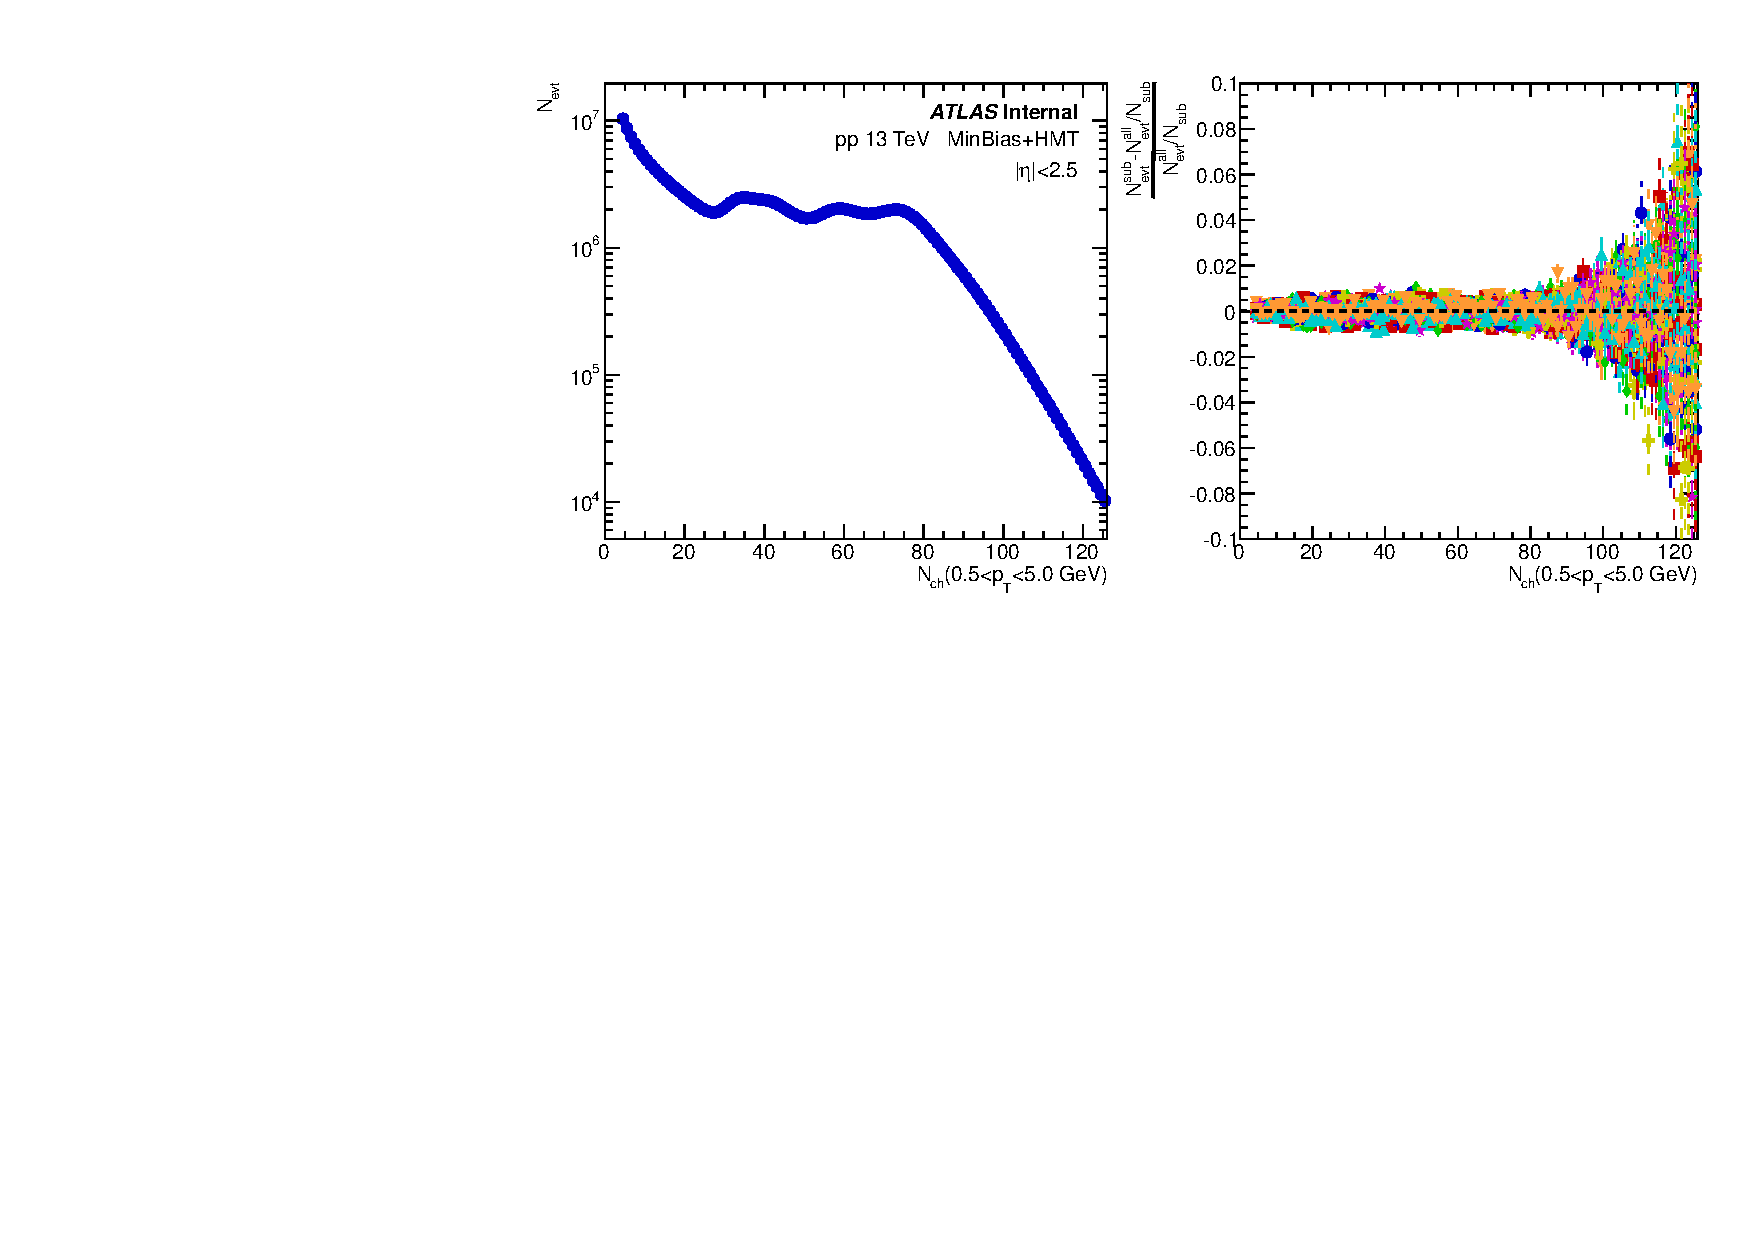
\includegraphics[width=.9\linewidth]{figs/sec_ana/pp13_chk_division.pdf}
\caption{$N_{ch}$ distribution for the whole 13 TeV $pp$ data sample (left); Right plot shows the relative difference of the statistics between sub-samples (indicated by different markers and colors) and the mean ($5\%$ statistics of the whole sample). The results are shown as a function of $N_{ch}$.}
\label{fig:ana_div}
\end{figure}

Then the $2k$-particle cumulant are calculated in whole sample, as well as in each sub-sample respectively. The standard deviation of cumulants calculated from all sub-samples are quoted as the statistical uncertainty of the cumulant for the whole sample.



\clearpage

\section{Systematics and cross-checks}
\label{sec:sys}
\subsection{Outline}
The systematics and cross-checks are presented in this section, with relative errors $\delta$ calculated in the following two scenarios:
\begin{itemize}
\item if one check is to compare with default: $\delta\equiv\frac{\mathcal{O}_\text{check}-\mathcal{O}_\text{default}}{\mathcal{O}_\text{default}}$;
\item if two checks (from sub-samples) are compared with each other: $\delta\equiv\frac{\mathcal{O}_\text{check 1}-\mathcal{O}_\text{check 2}}{\mathcal{O}_\text{check 1}+\mathcal{O}_\text{check 2}}$;
\end{itemize}
where $\mathcal{O}$ denotes the observable: 2-, 4- or 6-particle cumulant, and subscripts "default" and "check" are used to distinguish the different criteria.

The main systematic sources in this analysis are listed as follows:
\begin{itemize}
\item Monte-Carlo closure;
\item UCC trigger selection bias;
\item Loose v.s. tight track selection;
\item Low v.s. high tracking efficiency;
\item Impact of pileup rejection;
\item Flattening procedure;
\item Centrality definition;
\end{itemize}

The main cross-checks in this analysis are listed as follows:
\begin{itemize}
\item Event class bin width;
\item $\eta$ gap for subevent;
\end{itemize}

For simplicity, only systematics in standard cumulant are discussed, with following $p_{\text{T}}$ ranges:
\begin{itemize}
\item $c_1\{4\}$: $1.8<p_{\text{T}}<5.0$ GeV;
\item $c_2\{4\}$: $0.5<p_{\text{T}}<5.0$ GeV;
\item $c_3\{4\}$: $0.5<p_{\text{T}}<5.0$ GeV;
\item $c_4\{4\}$: $0.5<p_{\text{T}}<5.0$ GeV;
\end{itemize}
and for UCC trigger efficiency and pileup rejection, only systematics in ultra-central events are shown. At the end of this section, the summary of systematics are shown for all the observables.



\subsection{Ultra-central collision trigger efficiency}
In order to have enough statistics to study the cumulant in ultra-central collisions, ultra-central collision (UCC) triggered events are included. The trigger efficiencies are evaluated for all the UCC triggers separately. In the FCal $E_\text{T}$ region where trigger efficiency is less than 1 (turn-on region), due to the different tracking reconstructions between online and offline, event selection bias might be introduced to the analysis.

As one example, Fig.~\ref{fig:sys_trigEff_eg} shows the FCal $E_{T}$ distributions from MinBias and one of the UCC triggers: \verb|HLT_hi_|\verb|th1_ucc_L1TE10000| (left). This UCC trigger provides $~2$ times statistics than the MinBias trigger, in high FCal $E_{T}$ region, while the other UCC triggers provides more than 5 times statistics. The right plot shows the trigger efficiency. During the data taking, both MinBias and UCC triggers are heavily prescaled (except for the UCC triggers with highest threshold, which is running un-prescaled in most of the runs), and this means that the number of recorded events passing both MinBias and UCC triggers are extremely small. In order to evaluate the efficiency, we define the trigger "efficiency" on the statistical level:
\begin{equation}
\epsilon\equiv \frac{\sum\text{(event passing UCC * prescale)}}{\sum\text{(event passing MinBias trigger * prescale)}}
\end{equation}
Since the efficiency is defined on the statistical level, at large FCal $E_{T}$, the efficiency saturates towards 1, but not exactly at 1, as shown in the right plot of Fig.~\ref{fig:sys_trigEff}. Due to the strong correlation between online and offline FCal $E_{T}$, the turn-on curve of UCC triggers are very sharp, meaning that the selection bias due to UCC triggers are minimal. To be conservative, we still determined the FCal $E_{T}$ cut at $80\%$ efficiency for 3 sets of UCC triggers:
\begin{itemize}
\item FCal $E_{T}$ cut = 4.209 TeV for \verb|th1|;
\item FCal $E_{T}$ cut = 4.364 TeV for \verb|th2|;
\item FCal $E_{T}$ cut = 4.541 TeV for \verb|th3|;
\end{itemize}
\begin{figure}[H]
\centering
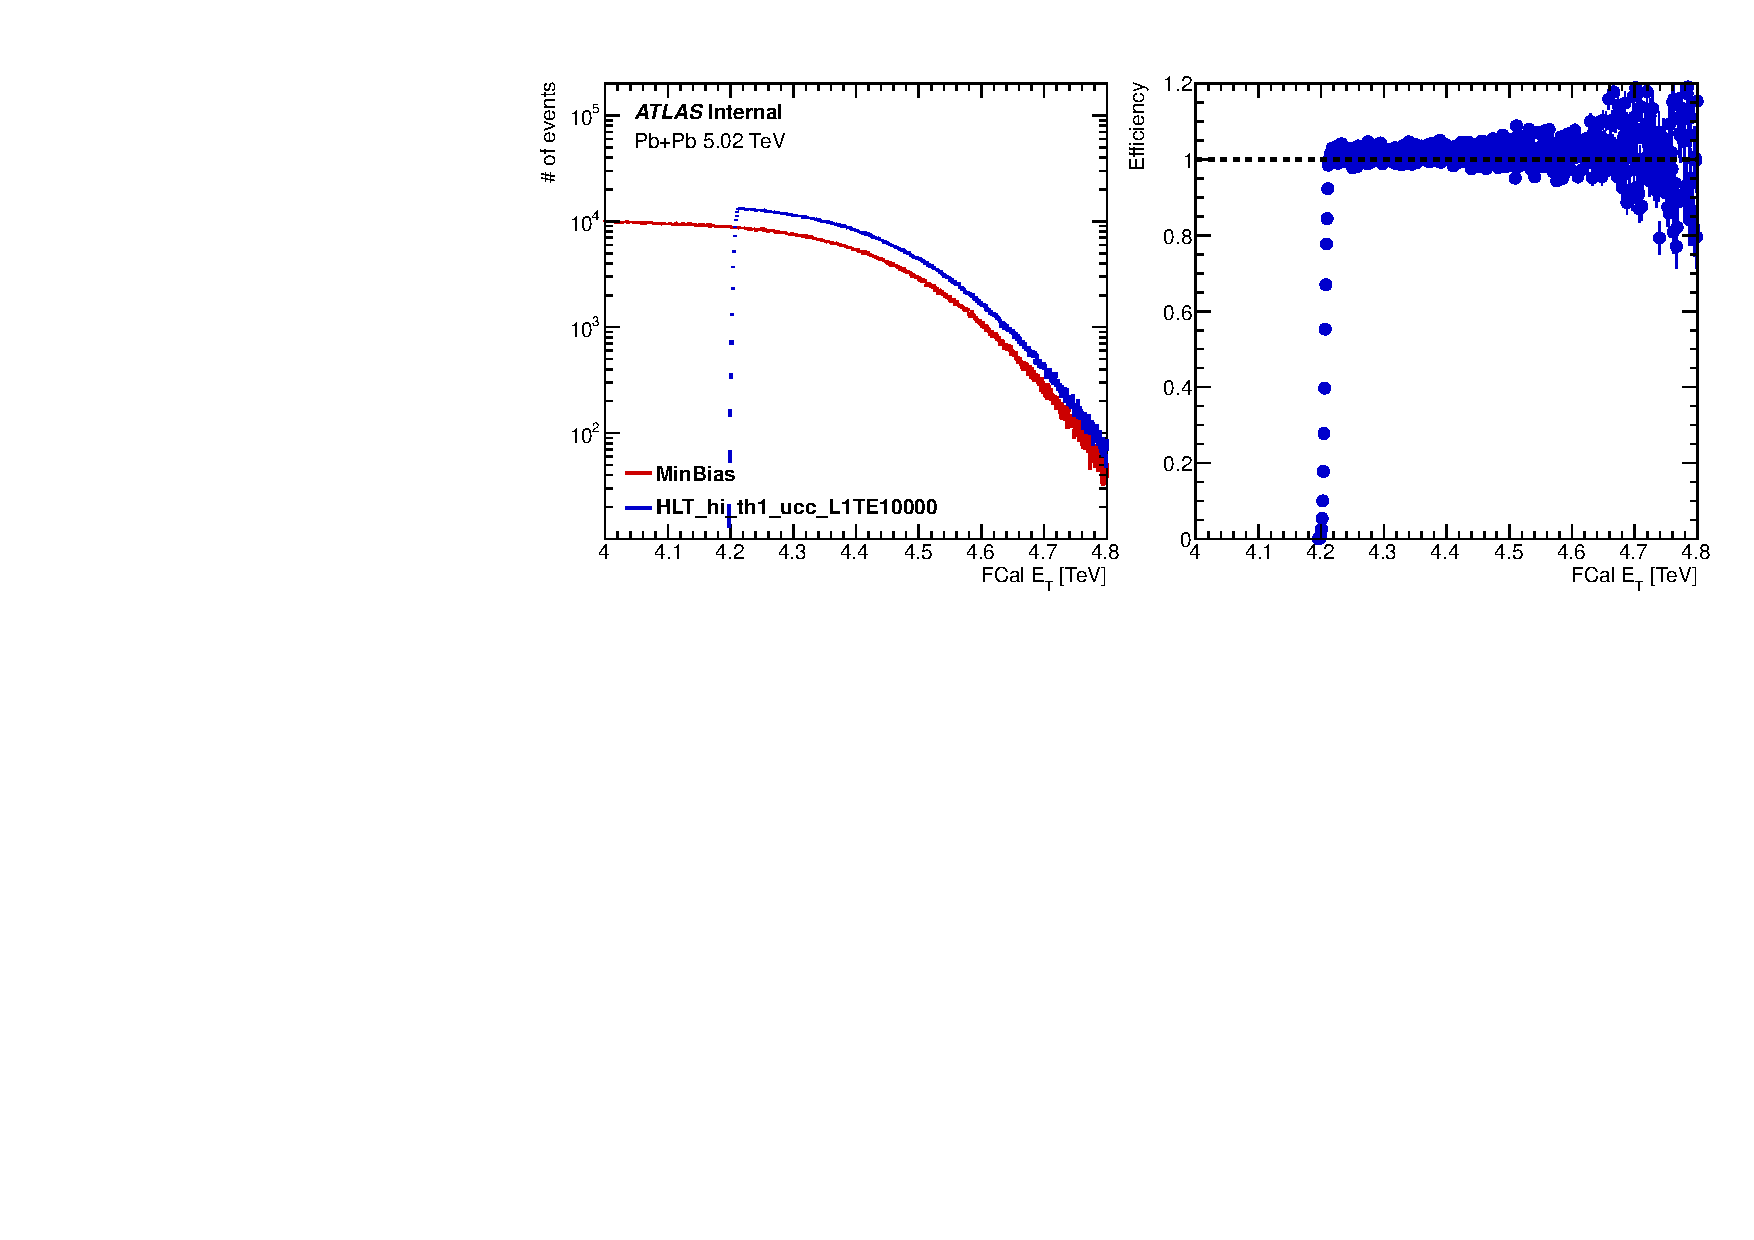
\includegraphics[width=.6\linewidth]{figs/sec_sys/trigEff_2.pdf}
\includegraphics[width=.3\linewidth]{figs/sec_sys/trigEff_zoom.pdf}
\caption{$N_{ch}$ distributions from MinBias and one UCC trigger (left), trigger "efficiency" as a function of FCal $E_{T}$ (middle) and a zoomed-in version (right) to better see the plateau.}
\label{fig:sys_trigEff_eg}
\end{figure}

In order to evaluate the potential selection bias, we performed the following two checks:
\begin{itemize}
\item Default: include UCC events with efficiency higher than $80\%$;
\item Check: include all UCC events;
\end{itemize}

Fig.~\ref{fig:sys_trigEff} shows the comparison of $c_n\{4\}$ calculated with (default) and without (check) the trigger efficiency selection, as a function of FCal $E_{T}$ in central collision (Note UCC triggers have no impact on events with centrality $>1\%$). For all the four harmonics, the relative uncertainties are much smaller compared with statistical uncertainties. This is as expected because the turn-on curve of the trigger efficiency is very sharp: not many events are rejected because of the $80\%$ trigger efficiency selection.
\begin{figure}[H]
\centering
\includegraphics[width=.245\linewidth]{figs/sec_appendix/sys_PbPb502_UCC/PbPb502_sys12_1sub_Har1_Pt5.pdf}
\includegraphics[width=.245\linewidth]{figs/sec_appendix/sys_PbPb502_UCC/PbPb502_sys12_1sub_Har2_Pt0.pdf}
\includegraphics[width=.245\linewidth]{figs/sec_appendix/sys_PbPb502_UCC/PbPb502_sys12_1sub_Har3_Pt0.pdf}
\includegraphics[width=.245\linewidth]{figs/sec_appendix/sys_PbPb502_UCC/PbPb502_sys12_1sub_Har4_Pt0.pdf}
\caption{Systematics of $c_n\{4\}$ from UCC trigger efficiency: with v.s. without trigger efficiency cut. Bottom panels are the relative uncertainties between the default and check.}
\label{fig:sys_trigEff}
\end{figure}

Due to much smaller systematic uncertainty compared with statistical uncertainty, trigger efficiency cut will not be quoted as part of the systematics.



\subsection{Monte-Carlo closure}
The HIJING Monte Carlo simulations were used to evaluate the difference between multi-particle cumulants in Pb+Pb data calculated using the generated and reconstructed charged particles obtained using the same analysis method. In some analysis it is considered as a crosscheck, since it assesses the quality of tracking, which are separately accounted for in previous systematics. The argument for not accounting it as a systematic uncertainties also relies on the fact that MC generators do not properly describe the investigated particle correlations. However, in this analysis, we are conservative to include the Monte-Carlo closure as part of the systematics.

Four million HIJING events with flow after-burner implemented are used for the MC closure (more details in \verb|ATLHI-116|). Note that both tracking and FCal $E_{T}$ are different between generated (truth) and reconstructed events, but in order to only evaluate the impact from offline tracking reconstruction, reconstructed FCal $E_{T}$, should be used for binning in both generated and reconstructed. Otherwise the differences between generated and reconstructed FCal $E_{T}$ will convolute with the tracking reconstruction, and that is not the purpose of this systematic check. However, the Monte-Carlo samples are generated using fast MC simulation configurations, which creates discrepancy of Calorimeter $E_{T}$ between data and MC. Due to this reason, the closure test was first binned in $N_{ch}^{rec}$, which is consistent with data, then mapped to the FCal $\lr{E_T}$ of data. In this case, the mismatch of FCal $E_{T}$ between data and MC plays little role. The procedure is similar as the Run 2 $v_n$ analysis~\cite{Burka:2151932}.

For the reconstructed tracks, it is not required to be associated with truth track, and both efficiency and fake rates are needed for the correction. Meanwhile, we do observe that the average of $\phi$ distribution is not very uniform in reconstructed tracks due to the simulation of detector effects, so flattening procedure is also applied in this Monte-Carlo check. In summary, all the corrections that has been applied in data analysis are also repeated with the Monte-Carlo test.

Fig.~\ref{fig:sys_mc} shows the $c_n\{4\}$ calculated from generated and reconstructed particles. Since the HIJING sample has flow implemented, both $c_2\{4\}$ and $c_3\{4\}$ show similar centrality dependence as data: largest in mid-central and approaches $0$ in central and peripheral. The relative differences are largest in central: reaching $3\%$, even after the efficiency and fake corrections are applied to the reconstructed tracks. As to $c_1\{4\}$ and $c_4\{4\}$, the centrality dependence is very different compared with data and the statistical errors are quite large. Due to these reasons, relative differences for $c_1\{4\}$ and $c_4\{4\}$ are not quoted as part of the systematics.
\begin{figure}[H]
\centering
\includegraphics[width=.245\linewidth]{figs/sec_sys/summary/sys5_c4_1sub_Har2_Pt0.pdf}
\includegraphics[width=.245\linewidth]{figs/sec_sys/summary/sys5_c4_1sub_Har3_Pt0.pdf}
\includegraphics[width=.245\linewidth]{figs/sec_sys/summary/sys5_c4_1sub_Har2_Pt1.pdf}
\includegraphics[width=.245\linewidth]{figs/sec_sys/summary/sys5_c4_1sub_Har3_Pt1.pdf}
\caption{Systematics of $c_n\{4\}$ from MC closure: generated v.s. reconstructed. Bottom panels are the relative uncertainties between the default and check. Note that the relative difference for $c_1\{4\}$ and $c_4\{4\}$ are set to be 0 (see main text).}
\label{fig:sys_mc}
\end{figure}

In addition, we have tested the following checks trying to diminish the $10\%$ differences observed in $c_2\{4\}$ and $c_3\{4\}$:
\begin{itemize}
\item Using a different 0.5 million HIJING sample (see in \verb|ATLHI-84|): similar outcome;
\item Do not apply efficiency or fake correction to reconstructed tracks: larger difference;
\item Only apply tracking efficiency: larger difference in central;
\item Apply flattening procedure on reconstructed tracks: similar outcome;
\item Apply additional $d_0$ and $z_0$ significance cuts to reconstructed tracks: larger difference;
\end{itemize}
Unfortunately, average efficiency and fake corrections will not compensate the inefficiency of reconstruction of tracks. To be conservative, the relative differences are quoted as systematics for both $c_2\{4\}$ and $c_3\{4\}$. As to the systematics in ultra-central collisions, since this HIJING sample does not contain enough ultra-central events, the systematic errors in UCC events are quoted from the plots above (error from the most central bin).

Since HIJING simulation does not implement correlation between flow harmonics, as shown in Fig.~\ref{fig:sys_mc_sc}(the signals are much smaller compared with data), systematics from MC closure for symmetric and asymmetric cumulant are set to be 0.
\begin{figure}[H]
\centering
\includegraphics[width=.245\linewidth]{figs/sec_sys/summary/sys5_sc_1sub_Har2_Pt0.pdf}
\includegraphics[width=.245\linewidth]{figs/sec_sys/summary/sys5_sc_1sub_Har3_Pt0.pdf}
\caption{Systematics of symmetric cumulants from MC closure: generated v.s. reconstructed. Bottom panels are the relative uncertainties between the default and check. Note that the relative differences are set to be 0 (see main text).}
\label{fig:sys_mc_sc}
\end{figure}



\subsection{Loose and tight track selection}
As default, the heavy ion loose track quality cut is applied in this analysis. In order to check stability of the track selection cuts, analysis is also repeated with tight track quality cut:
\begin{itemize}
\item Default: HI loose quality cut;
\item Check: HI tight quality cut;
\end{itemize}
where the definitions of loose and tight are listed in Section.~\ref{sec:trkSel}.

Fig.~\ref{fig:sys_trkSel} compares the $c_n\{4\}$ calculated with HI loose and tight track selection. For $c_2\{4\}$ and $c_3\{4\}$, the relative differences are within $3\%$ for all centralities. While for $c_1\{4\}$ and $c_4\{4\}$, since the signal is much smaller, the relative errors go up to $10\%$, but still within statistical uncertainties. This is not surprising because even though different track selections give different fake rates, they are already corrected using Monte-Carlo. Systematics from track selection are quoted as part of the combined systematics, for all the harmonics.
\begin{figure}[H]
\centering
\includegraphics[width=.245\linewidth]{figs/sec_appendix/sys_PbPb502/PbPb502_sys3_1sub_Har1_Pt5.pdf}
\includegraphics[width=.245\linewidth]{figs/sec_appendix/sys_PbPb502/PbPb502_sys3_1sub_Har2_Pt0.pdf}
\includegraphics[width=.245\linewidth]{figs/sec_appendix/sys_PbPb502/PbPb502_sys3_1sub_Har3_Pt0.pdf}
\includegraphics[width=.245\linewidth]{figs/sec_appendix/sys_PbPb502/PbPb502_sys3_1sub_Har4_Pt0.pdf}
\caption{Systematics of $c_n\{4\}$ from track selections: HI loose v.s. HI tight. Bottom panels are the relative uncertainties between the default and check.}
\label{fig:sys_trkSel}
\end{figure}



\subsection{Lower and higher tracking efficiency}
In this analysis, tracking efficiency is evaluated as a function of $p_\text{T}$, $\eta$ and centrality. Previous flow measurements have shown that $v_n$ strongly depends on $p_\text{T}$: it increases then decreases as $p_\text{T}$ increases. Meanwhile, differential flow measurements also shows that $v_n$ is weakly dependent of $\eta$. Due to these reasons, the $p_\text{T}$ weighting in tracking efficiency could introduce uncertainty to the results.

To evaluate the impact from uncertainty in the tracking efficiency, the following checks are performed:
\begin{itemize}
\item Default $\epsilon$: particles weighted by tracking efficiency;
\item Check 1 higher efficiency $\epsilon_+$: tracking efficiency in high $p_\text{T}$ is increased to its maximum within uncertainty; while tracking efficiency in low $p_\text{T}$ is decreased to its minimum within uncertainty;
\item Check 2 lower efficiency $\epsilon_-$: tracking efficiency in high $p_\text{T}$ is decreased to its minimum within uncertainty; while tracking efficiency in low $p_\text{T}$ is increased to its maximum within uncertainty;
\end{itemize}
where the two checks can be parameterized as:
\begin{equation}
\epsilon_\pm(p_\text{T}) \equiv \epsilon(p_\text{T}) \pm 0.06\frac{\epsilon(p_\text{T})-\epsilon(p_\text{T}^\text{low})}{\epsilon(p_\text{T}^\text{high})-\epsilon(p_\text{T}^\text{low})} \mp 0.03
\end{equation}
where $p_\text{T}^\text{low}$ is 0.5 GeV while $p_\text{T}^\text{high}$ is 5.0 GeV, which are the minimum and maximum $p_{T}$ ranges of this analysis.

\begin{figure}[H]
\centering
\includegraphics[width=.9\linewidth]{figs/sec_sys/sys_tracking_error.png}
\caption{The systematic uncertainties of the tracking efficiency plotted as a function of $p_\text{T}$ for several $|\eta|$ slices. These include the material uncertainties. These were obtained from the 13 TeV multiplicity analysis.~\cite{Morley:2011604}}
\label{fig:sys_tracking_error}
\end{figure}
Note that $0.03$ was selected as the variation of the tracking efficiency, which has been evaluated in the Minimum Bias multiplicity in 13 TeV $pp$ analysis~\cite{Morley:2011604}. The total uncertainty in tracking is shown in Fig.~\ref{fig:sys_tracking_error}, and the maximum variation for $p_\text{T}>0.5$ GeV is about $3\%$.

Fig.~\ref{fig:sys_trkEffLow} and fig.~\ref{fig:sys_trkEffHigh} show the comparison of $c_n\{4\}$ calculated using default tracking efficiency and lower/higher variations. For all the harmonics, the relative differences have opposite sign between lower and higher efficiency, as expected due to the $p_\text{T}$ dependence of flow. The largest relative differences come from low $p_\text{T}$ range, and decrease quickly as minimum $p_\text{T}$ cut increase. This check will be quoted as part of the combined systematics.
\begin{figure}[H]
\centering
\includegraphics[width=.245\linewidth]{figs/sec_sys/summary/sys1_c4_1sub_Har2_Pt0.pdf}
\includegraphics[width=.245\linewidth]{figs/sec_sys/summary/sys1_c4_1sub_Har3_Pt0.pdf}
\includegraphics[width=.245\linewidth]{figs/sec_sys/summary/sys1_c4_1sub_Har2_Pt1.pdf}
\includegraphics[width=.245\linewidth]{figs/sec_sys/summary/sys1_c4_1sub_Har3_Pt1.pdf}
\caption{Systematics of $c_n\{4\}$ from tracking efficiency: default v.s. lower efficiency. Bottom panels are the relative uncertainties between the default and check.}
\label{fig:sys_trkEffLow}
\end{figure}

\begin{figure}[H]
\centering
\includegraphics[width=.245\linewidth]{figs/sec_sys/summary/sys2_c4_1sub_Har2_Pt0.pdf}
\includegraphics[width=.245\linewidth]{figs/sec_sys/summary/sys2_c4_1sub_Har3_Pt0.pdf}
\includegraphics[width=.245\linewidth]{figs/sec_sys/summary/sys2_c4_1sub_Har2_Pt1.pdf}
\includegraphics[width=.245\linewidth]{figs/sec_sys/summary/sys2_c4_1sub_Har3_Pt1.pdf}
\caption{Systematics of $c_n\{4\}$ from tracking efficiency: default v.s. higher efficiency. Bottom panels are the relative uncertainties between the default and check.}
\label{fig:sys_trkEffHigh}
\end{figure}



\subsection{Pileup rejection}
During the 2015 Pb+Pb data taking, the mean value of $\mu$ is around 0.001, which means the fraction of pileup events is very low compared with $pp$ or $p+$Pb samples. Furthermore, in this analysis all the tracks used to calculate cumulants are from the primary vertex. In principle, in pile-up events, tracks from pile-up vertex should not contribute to the measurement. However, in the track and vertex reconstruction, when a pile-up vertex is too close to the primary vertex, two vertices might be merged. Since the particles from two different vertices are totally uncorrelated, including these events with merged vertex will reduce the signal of flow signal.

In order to check the impact from pileup events, a variation of pileup cleaning is performed:
\begin{itemize}
\item Default: official HI pileup rejection tool, based on FCal $E_T$ and ZDC;
\item Check: alternative pileup rejection method, based on FCal $E_T$ and tracks $N_{ch}$;
\end{itemize}

Fig.~\ref{fig:sys_pu_eg} illustrates the differences between the two pileup cleaning methods: official (left) and alternative (right). The left panel shows the correlation between FCal sum $E_T$ and calibrated number of neutrons in the ZDC. The main band (light blue circle) is dominated by the events with a single primary vertex and the "grass" above the main band (light red circle) are mainly from pileup events. This is because both the sum $E_T$ and number of neutrons in a pileup event are larger than the corresponding single event. In order to clean up the pileup events, a significance cut (indicated by the red curve) was applied to reject the top $0.1\%$ events at each FCal sum $E_T$ slice. From this correlation map, it is obvious that the pileup events and single events are disentangled at very high FCal sum $E_T$, meaning that almost all the pileup events are rejected with the official pileup tool. As a comparison, the right panel shows the correlation between FCal sum $E_T$ and the number of tracking efficiency corrected reconstructed tracks $N_{ch}$. Similar as the left panel, the "grass" under the main band are from the pileup events. However, since FCal sum $E_T$ and $N_{ch}$ are correlated, the overlap region between the pileup events and single events is much larger than the previous case, where the $N_\text{neutron}$ and FCal sum $E_T$ are anti-correlated. This means the performance of this alternative pileup rejection method is much worse than the official, which provides sufficient variations as a cross-check.
\begin{figure}[H]
\centering
\includegraphics[width=.9\linewidth]{figs/sec_sys/pu_eg.png}
\caption{An illustration of two pileup rejection methods: official HI pileup tool (left) and private pileup rejection (right).}
\label{fig:sys_pu_eg}
\end{figure}

The fraction of pileup events in peripheral is minimal and it increases fast with FCal $E_{T}$, so only comparisons in UCC events are shown. But note that this systematic check is also performed for the whole centrality range. It is worth mentioning that this check overestimates the pileup impact since the fraction of residual pileup events are large using the alternative rejection. Another way to estimate the impact from pileup would be by adjusting the significance cut of $N_\text{neutrons}$, and check the trend of $c_n\{4\}$ as a function of various ZDC energy cut. To be conservative, we are quoting the difference between the two methods as the upper bond of the systematics for pileup effects.

The comparison of $c_n\{4\}$ calculated with and without pileup rejection is shown in Fig.~\ref{fig:sys_pu}, as a function of FCal $E_{T}$ in ultra-central collisions. For all the harmonics, the relative differences are within $10\%$ and within statistical uncertainties. It is quoted as part of the systematics.

\begin{figure}[H]
\centering
\includegraphics[width=.245\linewidth]{figs/sec_appendix/sys_PbPb502_UCC/PbPb502_sys4_1sub_Har1_Pt5.pdf}
\includegraphics[width=.245\linewidth]{figs/sec_appendix/sys_PbPb502_UCC/PbPb502_sys4_1sub_Har2_Pt0.pdf}
\includegraphics[width=.245\linewidth]{figs/sec_appendix/sys_PbPb502_UCC/PbPb502_sys4_1sub_Har3_Pt0.pdf}
\includegraphics[width=.245\linewidth]{figs/sec_appendix/sys_PbPb502_UCC/PbPb502_sys4_1sub_Har4_Pt0.pdf}
\caption{Systematics of $c_n\{4\}$ from pileup effects: with s.s. without pileup rejection. Bottom panels are the relative uncertainties between the default and check.}
\label{fig:sys_pu}
\end{figure}



\subsection{Detector effects from flattening procedure}
Tracking efficiency weighting corrects the possible detector effects as a function of $\eta$ and $p_\text{T}$ , but the residual detector effects could still remain in the $\phi$ direction. In heavy ion collision, since the ”event plane” angle is random from event to event, the $\phi$ distribution averaged over many events should be flat and the discrepancy is due to the detector effects.

To estimate the impact from detector effects, the flattening produce was performed. The correction factor, $w_\phi$, is defined as:
\begin{equation}
w_\phi(\eta,\phi)\equiv\frac{\lr{N(\delta\eta)}}{N(\delta\eta,\delta\phi)}
\end{equation}
where $N(\delta\eta,\delta\phi)$ is the number of particles in the small $(\eta,\phi)$ phase-space window; and $\lr{N(\delta\eta)}$ is the mean number of particles in the small $\eta$ slice averaged over the whole $\phi$ range. $w_\phi$ is evaluated run-by-run, as a function of $p_\text{T}$, vertex position $z_{vtx}$ and charge, so that it can properly correct the detector effects.

To illustrate how the flattening works, Fig.~\ref{fig:sys_flat_eg} shows the $\eta-\phi$ distributions before (left) and after (right) flattening. Several holes are observed in the raw $\eta-\phi$ distribution, while after flattening, the average $\phi$ distribution is flat by construction in each $\eta$ slice.
\begin{figure}[H]
\centering
\includegraphics[width=1.\linewidth]{figs/sec_ana/cumuFlat_Cent0_Zvtx5_Chg0_Pt1.pdf}
\caption{An example demonstrating how flattening works. Left plot is the raw $\eta-\phi$ distribution, while right plot is the $\eta-\phi$ distribution after flattening procedure. Middle panel shows the correction factor $w_\phi$.}
\label{fig:sys_flat_eg}
\end{figure}

To check the impact from flattening correction, we have performed:
\begin{itemize}
\item Default: each particle weighted by $w_\phi$;
\item Check: particles not weighted by $w_\phi$;
\end{itemize}

A comparison of $c_n\{4\}$ before and after flattening is shown in Fig.~\ref{fig:sys_flat}. For all the harmonics, the relative differences are within $10\%$ and within statistical uncertainties. However, the relative difference seems to increase towards the central collision. Since the detector effect indeed depends on the occupancy of detector, it is worth checking the impact from flattening in UCC in details.
\begin{figure}[H]
\centering
\includegraphics[width=.245\linewidth]{figs/sec_appendix/sys_PbPb502/PbPb502_sys11_1sub_Har1_Pt5.pdf}
\includegraphics[width=.245\linewidth]{figs/sec_appendix/sys_PbPb502/PbPb502_sys11_1sub_Har2_Pt0.pdf}
\includegraphics[width=.245\linewidth]{figs/sec_appendix/sys_PbPb502/PbPb502_sys11_1sub_Har3_Pt0.pdf}
\includegraphics[width=.245\linewidth]{figs/sec_appendix/sys_PbPb502/PbPb502_sys11_1sub_Har4_Pt0.pdf}
\caption{Systematics of $c_n\{4\}$ from flattening procedure: with and without flattening. Bottom panels are the relative uncertainties between the default and check.}
\label{fig:sys_flat}
\end{figure}

A comparison of $c_n\{4\}$ in ultra-central collisions before and after flattening is shown in Fig.~\ref{fig:sys_flat_UCC}. For the odd harmonics $c_1\{4\}$ and $c_3\{4\}$, flattening does not change the results too much: the relative differences are within $10\%$ and still within statistical errors. However, for the even harmonics, especially for $c_2\{4\}$, the positive magnitude without flattening is smaller than default. Since the flattening is an essential procedure to account for the detector effects. This check will be quoted as the systematics.
\begin{figure}[H]
\centering
\includegraphics[width=.245\linewidth]{figs/sec_appendix/sys_PbPb502_UCC/PbPb502_sys11_1sub_Har1_Pt5.pdf}
\includegraphics[width=.245\linewidth]{figs/sec_appendix/sys_PbPb502_UCC/PbPb502_sys11_1sub_Har2_Pt0.pdf}
\includegraphics[width=.245\linewidth]{figs/sec_appendix/sys_PbPb502_UCC/PbPb502_sys11_1sub_Har3_Pt0.pdf}
\includegraphics[width=.245\linewidth]{figs/sec_appendix/sys_PbPb502_UCC/PbPb502_sys11_1sub_Har4_Pt0.pdf}
\caption{Systematics of $c_n\{4\}$ in ultra-central collisions from flattening procedure: with and without flattening. Bottom panels are the relative uncertainties between the default and check.}
\label{fig:sys_flat_UCC}
\end{figure}

A proper way to estimate the residual detector effects after flattening should be through mixed events technique, as has been discussed in Sec.~\ref{sec:ana}.



\subsection{Centrality definition}
Uncertainty in how well the min-bias triggers sample the Pb+Pb cross-section (i.e. the min-bias trigger efficiency) results in an uncertainty in the definition of the centrality intervals. This causes the nominal $(0-85)\%$ centrality range to have a $\pm 1\%$ uncertainty. The effect of such uncertainties on observables are determined by re-evaluating the observables with the following criteria:
\begin{itemize}
\item Default: $(0-85)\%$ centrality range;
\item Check 1: $(0-84)\%$ centrality range;
\item Check 2: $(0-86)\%$ centrality range;
\end{itemize}

\begin{figure}[H]
\centering
\includegraphics[width=.245\linewidth]{figs/sec_sys/summary/sys7_c4_1sub_Har2_Pt0.pdf}
\includegraphics[width=.245\linewidth]{figs/sec_sys/summary/sys7_c4_1sub_Har3_Pt0.pdf}
\includegraphics[width=.245\linewidth]{figs/sec_sys/summary/sys7_c4_1sub_Har2_Pt1.pdf}
\includegraphics[width=.245\linewidth]{figs/sec_sys/summary/sys7_c4_1sub_Har3_Pt1.pdf}
\caption{Systematics of $c_n\{4\}$ from centrality definition: $(0-85)\%$ v.s. $(0-84)\%$ . Bottom panels are the relative uncertainties between the default and check.}
\label{fig:sys_cent}
\end{figure}
Fig.~\ref{fig:sys_cent} compares the $c_n\{4\}$ for the different centrality ranges. This systematic uncertainty depends on the centrality dependence of the observable: if the observable has no centrality dependence, the uncertainty is zero. On the other hand, this uncertainty is large if the observable is strongly dependent of centrality. This explains why this uncertainty for $c_3\{4\}$ is larger than that of $c_2\{4\}$. Different $p_\text{T}$ ranges make little difference since the relative centrality dependence of the observables do not change much.



\subsection{Event class bin width}
As has been discussed in Sec.~\ref{sec:ana}, cumulant is sensitive to the definition of event class, which is associated with the multiplicity fluctuation. In order to suppress the multiplicity fluctuation, while calculating the multi-particle correlation, the events are always binned with $1\%$ centrality bin width, which is sufficient for cumulant-like analysis~\cite{Jia:2017hbm}. However, unlike in small systems, since the non-flow contribution is much smaller in Pb+Pb collisions, different bin widths will not trigger non-flow fluctuations. However, different bin widths could still result in different flow fluctuations, especially when the bin width is too large. So it is worthwhile to check the impact of event class bin width:
\begin{itemize}
\item default: $1\%$ centrality as the event class bin width;
\item check: $5\%$ centrality as the event class bin width;
\end{itemize}

Fig.~\ref{fig:sys_binWidth} shows the comparison of $c_n\{4\}$ calculated with two event class bin widths. For the lower harmonics $c_1\{4\}$ and $c_2\{4\}$, the relative differences are within statistics errors. While for the higher order harmonics $c_3\{4\}$ and $c_4\{4\}$, since flow signal is smaller, the flow fluctuation becomes larger. This explains why the relative differences of $c_3\{4\}$ and $c_4\{4\}$ between two event class bin widths are larger. This cross-check illustrates the importance of narrow bin width in the cumulant calculation, but it will NOT be quoted as part of the systematics since we will always use the narrowest bin width.
\begin{figure}[H]
\centering
\includegraphics[width=.245\linewidth]{figs/sec_appendix/sys_PbPb502/PbPb502_sys6_1sub_Har1_Pt5.pdf}
\includegraphics[width=.245\linewidth]{figs/sec_appendix/sys_PbPb502/PbPb502_sys6_1sub_Har2_Pt0.pdf}
\includegraphics[width=.245\linewidth]{figs/sec_appendix/sys_PbPb502/PbPb502_sys6_1sub_Har3_Pt0.pdf}
\includegraphics[width=.245\linewidth]{figs/sec_appendix/sys_PbPb502/PbPb502_sys6_1sub_Har4_Pt0.pdf}
\caption{Systematics of $c_n\{4\}$ from different bin width: $1\%$ v.s. $5\%$ centrality bin widths. Bottom panels are the relative uncertainties between the default and check.}
\label{fig:sys_binWidth}
\end{figure}



\subsection{$\eta$ gap for subevent}
Compared with 2-subevent method, 3-subevent method is designed to remove the dijet-like correlation, where the chance that both jets contribute to all the 3 subevents are dramatically lowered. The only situation where dijet correlation still contributes is when two jets fall upon the two boundaries among 3 subevents. To show whether the $c_n\{4\}$ is affected by the residual dijet contributions, we introduced $\eta$ gaps between subevents.

Fig.~\ref{fig:sys_etaGap_eg} is a cartoon showing how the $\eta$ gap was applied to the subevent methods. For the standard cumulant method, in principle $\eta$ gap can also be applied among all 4 particles. However, the formula of direct cumulant will no longer hold and one has to rely on the nested loop method. Meanwhile for the subevent methods, it is quite natural to apply the $\eta$ gaps between subevents, while keeping the formula the same. In the following cross-checks, we will only test the $\eta$ gap in subevent methods. After all, the subevent method is used to evaluate the residual non-flow in Pb+Pb, and if subevent cumulant with $\eta$ gap gives consistent results, it means most of the dijet-like non-flow are already removed by the 3-subevent method.

\begin{figure}[H]
\centering
\includegraphics[width=.9\linewidth]{figs/sec_sys/etaGap_eg.png}
\caption{A cartoon showing how the $\eta$ gap was applied to subevent to further suppress the long-range non-flow.}
\label{fig:sys_etaGap_eg}
\end{figure}

Fig.~\ref{fig:sys_etaGap} presents the comparisons of $c_n\{4\}$ with and without $\eta=0.5$ gap, calculated using 3-subevent methods. For $c_2\{4\}$, since the elliptic flow is dominating over the non-flow, applying $\eta$ gap has minimal impact on the results. While for $c_3\{4\}$ and $c_4\{4\}$, where the flow signals become smaller, subevent with $\eta$ gap causes up to $10\%$ difference compared with no gap. In the end, since $c_1\{4\}$ signal is even smaller, by applying the $\eta$ gap, the number of particle combinations in $\lr{4}$ will drop, which results in larger statistical errors. Since the residual non-flow upon subevent cumulant is under control, this cross-check will NOT be quoted as systematics. To increase statistical significance, the default subevent method will NOT include the $\eta$ gap.
\begin{figure}[H]
\centering
\includegraphics[width=.245\linewidth]{figs/sec_appendix/sys_PbPb502/PbPb502_sys7_3sub_Har1_Pt5.pdf}
\includegraphics[width=.245\linewidth]{figs/sec_appendix/sys_PbPb502/PbPb502_sys7_3sub_Har2_Pt0.pdf}
\includegraphics[width=.245\linewidth]{figs/sec_appendix/sys_PbPb502/PbPb502_sys7_3sub_Har3_Pt0.pdf}
\includegraphics[width=.245\linewidth]{figs/sec_appendix/sys_PbPb502/PbPb502_sys7_3sub_Har4_Pt0.pdf}
\caption{Systematics of $c_n\{4\}$ from $\eta$ gap between subevents: with $\eta=0.5$ gap and without gap. The $c_n\{4\}$ are calculated using 3-subevent method. Bottom panels are the relative uncertainties between the default and check.}
\label{fig:sys_etaGap}
\end{figure}



\subsection{Summary of systematics}
This section summarizes the breakdown of systematics for every observable in this analysis. In order not to flooding the plots, the results are shown in two $p_\text{T}$ ranges:
\begin{itemize}
\item $0.5<p_\text{T}<5.0$ GeV;
\item $1.0<p_\text{T}<5.0$ GeV;
\end{itemize}
and except for the 2-particle cumulant, all other results are only shown using standard cumulant method. The corresponding systematics from 3-subevent method is listed in the Appendix.

Overall, the summary of systematics has the following features:
\begin{itemize}
\item In most cases, systematics are dominated by tracking efficiency variations. This is not surprising since magnitude of flow, as well as its fluctuation, are highly dependent of $p_\text{T}$. Slightly change in tracking efficiency as a function of $p_\text{T}$ will cause noticeable differences to cumulants;
\item Monte-Carlo closure has significant impact on $c_n\{2k\}$: in the lower $p_\text{T}$ region, about $5\%$ for 2-particle cumulant, $10\%$ and $15\%$ for 4- and 6-particle cumulants. In higher $p_\text{T}$, systematics from MC closure become much smaller;
\item Normalized cumulant, symmetric cumulant and asymmetric cumulant have smaller systematic errors than its correspondence without normalization, due to the reason that part of the systematics are canceled out in the ratio;
\end{itemize}

As a summary, in most cases, the total systematics are within $10\%$. In other cases where the systematics are larger, they are still smaller or comparable with statistical uncertainties.

\subsubsection{2-particle cumulant $c_n\{2\}$}
\begin{figure}[H]
\centering
\includegraphics[width=.425\linewidth]{figs/sec_sys/summary/sys_c2_3sub_Har2_Pt0.pdf}
\includegraphics[width=.425\linewidth]{figs/sec_sys/summary/sys_c2_3sub_Har2_Pt1.pdf}
\includegraphics[width=.425\linewidth]{figs/sec_sys/summary/sys_c2_3sub_Har3_Pt0.pdf}
\includegraphics[width=.425\linewidth]{figs/sec_sys/summary/sys_c2_3sub_Har3_Pt1.pdf}
\includegraphics[width=.425\linewidth]{figs/sec_sys/summary/sys_c2_3sub_Har4_Pt0.pdf}
\includegraphics[width=.425\linewidth]{figs/sec_sys/summary/sys_c2_3sub_Har4_Pt1.pdf}
\caption{Breakdown of all major systematic sources for 2-particle cumulant $c_n\{2\}$. Left column shows the lower $p_\text{T}$ cut and right column shows the higher $p_\text{T}$ cut. Different rows represent different harmonics. The cumulants are calculated using standard method. Shaded area indicate the statistical uncertainty.}
\label{fig:sys_sum_c2}
\end{figure}

\subsubsection{4-particle cumulant $c_n\{4\}$ and $\hat{c}_n\{4\}$}
\begin{figure}[H]
\centering
\includegraphics[width=.425\linewidth]{figs/sec_sys/summary/sys_c4_1sub_Har2_Pt0.pdf}
\includegraphics[width=.425\linewidth]{figs/sec_sys/summary/sys_c4_1sub_Har2_Pt1.pdf}
\includegraphics[width=.425\linewidth]{figs/sec_sys/summary/sys_c4_1sub_Har3_Pt0.pdf}
\includegraphics[width=.425\linewidth]{figs/sec_sys/summary/sys_c4_1sub_Har3_Pt1.pdf}
\includegraphics[width=.425\linewidth]{figs/sec_sys/summary/sys_c4_1sub_Har4_Pt0.pdf}
\includegraphics[width=.425\linewidth]{figs/sec_sys/summary/sys_c4_1sub_Har4_Pt1.pdf}
\caption{Breakdown of all major systematic sources for 4-particle cumulant $c_n\{4\}$. Left column shows the lower $p_\text{T}$ cut and right column shows the higher $p_\text{T}$ cut. Different rows represent different harmonics. The cumulants are calculated using standard method. Shaded area indicate the statistical uncertainty.}
\label{fig:sys_sum_c4}
\end{figure}

\begin{figure}[H]
\centering
\includegraphics[width=.425\linewidth]{figs/sec_sys/summary/sys_nc4_1sub_Har2_Pt0.pdf}
\includegraphics[width=.425\linewidth]{figs/sec_sys/summary/sys_nc4_1sub_Har2_Pt1.pdf}
\includegraphics[width=.425\linewidth]{figs/sec_sys/summary/sys_nc4_1sub_Har3_Pt0.pdf}
\includegraphics[width=.425\linewidth]{figs/sec_sys/summary/sys_nc4_1sub_Har3_Pt1.pdf}
\includegraphics[width=.425\linewidth]{figs/sec_sys/summary/sys_nc4_1sub_Har4_Pt0.pdf}
\includegraphics[width=.425\linewidth]{figs/sec_sys/summary/sys_nc4_1sub_Har4_Pt1.pdf}
\caption{Breakdown of all major systematic sources for normalized 4-particle cumulant $\hat{c}_n\{4\}$. Left column shows the lower $p_\text{T}$ cut and right column shows the higher $p_\text{T}$ cut. Different rows represent different harmonics. The cumulants are calculated using standard method. Shaded area indicate the statistical uncertainty.}
\label{fig:sys_sum_nc4}
\end{figure}

\subsubsection{6-particle cumulant $c_n\{6\}$ and $\hat{c}_n\{6\}$}
\begin{figure}[H]
\centering
\includegraphics[width=.425\linewidth]{figs/sec_sys/summary/sys_c6_1sub_Har2_Pt0.pdf}
\includegraphics[width=.425\linewidth]{figs/sec_sys/summary/sys_c6_1sub_Har2_Pt1.pdf}
\includegraphics[width=.425\linewidth]{figs/sec_sys/summary/sys_c6_1sub_Har3_Pt0.pdf}
\includegraphics[width=.425\linewidth]{figs/sec_sys/summary/sys_c6_1sub_Har3_Pt1.pdf}
\includegraphics[width=.425\linewidth]{figs/sec_sys/summary/sys_c6_1sub_Har4_Pt0.pdf}
\includegraphics[width=.425\linewidth]{figs/sec_sys/summary/sys_c6_1sub_Har4_Pt1.pdf}
\caption{Breakdown of all major systematic sources for 6-particle cumulant $c_n\{6\}$. Left column shows the lower $p_\text{T}$ cut and right column shows the higher $p_\text{T}$ cut. Different rows represent different harmonics. The cumulants are calculated using standard method. Shaded area indicate the statistical uncertainty.}
\label{fig:sys_sum_c6}
\end{figure}

\begin{figure}[H]
\centering
\includegraphics[width=.425\linewidth]{figs/sec_sys/summary/sys_nc6_1sub_Har2_Pt0.pdf}
\includegraphics[width=.425\linewidth]{figs/sec_sys/summary/sys_nc6_1sub_Har2_Pt1.pdf}
\includegraphics[width=.425\linewidth]{figs/sec_sys/summary/sys_nc6_1sub_Har3_Pt0.pdf}
\includegraphics[width=.425\linewidth]{figs/sec_sys/summary/sys_nc6_1sub_Har3_Pt1.pdf}
\includegraphics[width=.425\linewidth]{figs/sec_sys/summary/sys_nc6_1sub_Har4_Pt0.pdf}
\includegraphics[width=.425\linewidth]{figs/sec_sys/summary/sys_nc6_1sub_Har4_Pt1.pdf}
\caption{Breakdown of all major systematic sources for normalized 6-particle cumulant $\hat{c}_n\{6\}$. Left column shows the lower $p_\text{T}$ cut and right column shows the higher $p_\text{T}$ cut. Different rows represent different harmonics. The cumulants are calculated using standard method. Shaded area indicate the statistical uncertainty.}
\label{fig:sys_sum_nc6}
\end{figure}

\subsubsection{Universality check of flow fluctuation}
\begin{figure}[H]
\centering
\includegraphics[width=.425\linewidth]{figs/sec_sys/summary/sys_isGauss_1sub_Har2_Pt0.pdf}
\includegraphics[width=.425\linewidth]{figs/sec_sys/summary/sys_isGauss_1sub_Har2_Pt1.pdf}
\includegraphics[width=.425\linewidth]{figs/sec_sys/summary/sys_isPower_1sub_Har2_Pt0.pdf}
\includegraphics[width=.425\linewidth]{figs/sec_sys/summary/sys_isPower_1sub_Har2_Pt1.pdf}
\caption{Breakdown of all major systematic sources for flow fluctuation check. Left column shows the lower $p_\text{T}$ cut and right column shows the higher $p_\text{T}$ cut. Different rows represent different fluctuation models. The cumulants are calculated using standard method. Shaded area indicate the statistical uncertainty.}
\label{fig:sys_sum_fluc}
\end{figure}

\subsubsection{Symmetric and normalized symmetric cumulant $sc_{n,m}\{4\}$ and $nsc_{n,m}\{4\}$}
\begin{figure}[H]
\centering
\includegraphics[width=.425\linewidth]{figs/sec_sys/summary/sys_sc_1sub_Har2_Pt0.pdf}
\includegraphics[width=.425\linewidth]{figs/sec_sys/summary/sys_sc_1sub_Har2_Pt1.pdf}
\includegraphics[width=.425\linewidth]{figs/sec_sys/summary/sys_sc_1sub_Har3_Pt0.pdf}
\includegraphics[width=.425\linewidth]{figs/sec_sys/summary/sys_sc_1sub_Har3_Pt1.pdf}
\caption{Breakdown of all major systematic sources for symmetric cumulant $sc_{n,m}\{4\}$. Left column shows the lower $p_\text{T}$ cut and right column shows the higher $p_\text{T}$ cut. Different rows represent different harmonic combinations. The cumulants are calculated using standard method. Shaded area indicate the statistical uncertainty.}
\label{fig:sys_sum_sc}
\end{figure}

\begin{figure}[H]
\centering
\includegraphics[width=.425\linewidth]{figs/sec_sys/summary/sys_nsc_1sub_Har2_Pt0.pdf}
\includegraphics[width=.425\linewidth]{figs/sec_sys/summary/sys_nsc_1sub_Har2_Pt1.pdf}
\includegraphics[width=.425\linewidth]{figs/sec_sys/summary/sys_nsc_1sub_Har3_Pt0.pdf}
\includegraphics[width=.425\linewidth]{figs/sec_sys/summary/sys_nsc_1sub_Har3_Pt1.pdf}
\caption{Breakdown of all major systematic sources for normalized symmetric cumulant $nsc_{n,m}\{4\}$. Left column shows the lower $p_\text{T}$ cut and right column shows the higher $p_\text{T}$ cut. Different rows represent different harmonic combinations. The cumulants are calculated using standard method. Shaded area indicate the statistical uncertainty.}
\label{fig:sys_sum_nsc}
\end{figure}

\subsubsection{Asymmetric and normalized asymmetric cumulant $ac_{n,n+m}\{3\}$ and $nac_{n,n+m}\{3\}$}
\begin{figure}[H]
\centering
\includegraphics[width=.425\linewidth]{figs/sec_sys/summary/sys_ac_1sub_Har2_Pt0.pdf}
\includegraphics[width=.425\linewidth]{figs/sec_sys/summary/sys_ac_1sub_Har2_Pt1.pdf}
\caption{Breakdown of all major systematic sources for asymmetric cumulant $ac_{n,n+m}\{3\}$. Left column shows the lower $p_\text{T}$ cut and right column shows the higher $p_\text{T}$ cut. The cumulants are calculated using standard method. Shaded area indicate the statistical uncertainty.}
\label{fig:sys_sum_ac}
\end{figure}

\begin{figure}[H]
\centering
\includegraphics[width=.425\linewidth]{figs/sec_sys/summary/sys_nac_1sub_Har2_Pt0.pdf}
\includegraphics[width=.425\linewidth]{figs/sec_sys/summary/sys_nac_1sub_Har2_Pt1.pdf}
\caption{Breakdown of all major systematic sources for normalized asymmetric cumulant $nac_{n,n+m}\{3\}$. Left column shows the lower $p_\text{T}$ cut and right column shows the higher $p_\text{T}$ cut. The cumulants are calculated using standard method. Shaded area indicate the statistical uncertainty.}
\label{fig:sys_sum_nac}
\end{figure}







\clearpage

\section{Results}
\label{sec:result}
\subsection{Outline}
In this section, all the main results for 5.02 TeV Pb+Pb are presented as follows:
\begin{itemize}
\item Comparison between standard and 3-subevent cumulant;
\item 2-particle cumulant $c_n\{2\}$;
\item 4-particle cumulant $c_n\{4\}$ and $nc_n\{4\}$;
\item 4-particle cumulant in ultra-central collisions;
\item 4-particle cumulant in 2.76 and 5.02 TeV;
\item 6-particle cumulant $c_n\{6\}$ and $nc_n\{6\}$;
\item Universality check of flow fluctuation models;
\item Symmetric cumulant $sc_{n,m}\{4\}$ and $nsc_{n,m}\{4\}$;
\item Asymmetric cumulant $ac_{n,n+m}\{3\}$ and $nac_{n,n+m}\{3\}$;
\end{itemize}
Most of the results are calculated using standard cumulant method, and they are presented in the following 4 $p_\text{T}$ ranges:
\begin{itemize}
\item $0.5<p_\text{T}<5.0$ GeV
\item $1.0<p_\text{T}<5.0$ GeV
\item $1.5<p_\text{T}<5.0$ GeV
\item $2.0<p_\text{T}<5.0$ GeV
\end{itemize}
In additional, three different event class definitions are applied to test impact of centrality on flow fluctuations:
\begin{itemize}
\item Event class definition 1: centrality: defined by FCal $E_\text{T}$;
\item Event class definition 2: FCal $E_\text{T}$: same as centrality but with better look in UCC;
\item Event class definition 3: $N_{ch}^{rec}$: different $\eta$ range from FCal $E_\text{T}$;
\end{itemize}

\subsection{Comparison between standard and 3-subevent cumulant}
3-subevent method was proposed to suppress the residual non-flow contribution. It measures particle correlation across different $\eta$ ranges. The method has been extensively studied in small systems and proven its effectiveness. However, in large systems like Pb+Pb collision, where flow signal is dominating over non-flow, the improvement from 3-subevent method is limited. In this section, we will make direct comparison between results using standard and 3-subevent methods. If the difference is not large, standard method will be the default method due to its smaller statistical uncertainties.

\begin{figure}[H]
\centering
\includegraphics[width=.95\linewidth]{figs/sec_result/forQM/mtd_c2.pdf}
\caption{$c_n\{2\}$ compared between standard and 3-subevent methods, with low $p_\text{T}$ (top) and high $p_\text{T}$ (bottom). Different columns are for different harmonics.}
\label{fig:result_mtd_c2}
\end{figure}
Fig.~\ref{fig:result_mtd_c2} compares the 2-particle cumulant $c_n\{2\}$ using two methods. For second-harmonic $v_2$, the differences between two methods are small in central and mid-central collisions. As the collision moves to peripheral, since number of particles deceases fast, the non-flow contributions case the growth of the differences between two methods. While for other flow harmonics, due to their smaller magnitudes, the suppression from 3-subevent method is observed even in central collision. The huge differences in $v_1$ is partially due to the large momentum conservation effects in standard method, which we will not discuss in details in this analysis ($c_1\{2\}$ is not included in the results). Since the statistical uncertainty for 2-particle correlation is not an issue, in order to suppress the non-flow, in this analysis, 3-subevent method is always preferred whenever 2-particle correlations are calculated (for example in the normalized cumulant).

\begin{figure}[H]
\centering
\includegraphics[width=.95\linewidth]{figs/sec_result/forQM/mtd_c4.pdf}
\caption{$c_n\{4\}$ compared between standard and 3-subevent methods, with low $p_\text{T}$ (top) and high $p_\text{T}$ (bottom). Different columns are for different harmonics.}
\label{fig:result_mtd_c4}
\end{figure}
Fig.~\ref{fig:result_mtd_c4} compares the 4-particle cumulant $c_n\{4\}$ using standard and 3-subevent methods. For $v_2$, both methods give very consistent $c_2\{4\}$. This is as expected since by requiring 4 particles in the correlation calculation, the non-flow contributions are already significantly suppressed. For $v_3$ and $v_4$, both methods are consistent within statistical uncertainties, and we do see the errors from 3-subevent are much larger. For $v_1$ in high $p_\text{T}$, 3-subevent method can also measure negative $c_1\{4\}$ in peripheral region, but with smaller statistical significance. This observation supports our claim that negative $c_1\{4\}$ is not due to non-flow contributions.

\begin{figure}[H]
\centering
\includegraphics[width=.95\linewidth]{figs/sec_result/forQM/mtd_nc4.pdf}
\caption{$nc_n\{4\}$ compared between standard and 3-subevent methods, with low $p_\text{T}$ (top) and high $p_\text{T}$ (bottom). Different columns are for different harmonics.}
\label{fig:result_mtd_nc4}
\end{figure}
Fig.~\ref{fig:result_mtd_nc4} shows the results for normalized 4-particle cumulant. Since both standard and 3-subevent cumulants are normalized by the 3-subevent 2-particle correlation, the behaviors of $nc_n\{4\}$ are the same as $c_n\{4\}$: both methods give consistent results. (Please ignore the leftmost column because $c_1\{2\}$ is not well defined.)

\begin{figure}[H]
\centering
\includegraphics[width=.95\linewidth]{figs/sec_result/forQM/mtd_sc.pdf}
\caption{Symmetric and asymmetric cumulant compared between standard and 3-subevent methods, with low $p_\text{T}$ (top) and high $p_\text{T}$ (bottom). Different columns are for different observables.}
\label{fig:result_mtd_sc}
\end{figure}
In the end, Fig.~\ref{fig:result_mtd_sc} compares the 2 methods for symmetric and asymmetric cumulants. For the observables shown in the figure, both methods began to deviate towards peripheral collisions. The differences can be caused by two factors: non-flow contributions and flow decorrelation effects. Flow decorrelation effects are introduced into 3-subevent method simply because 3 events are separated in the $\eta$ direction. Since in this analysis we do not tend to discuss such effects, the standard method is selected as the default one when presenting the symmetric and asymmetric cumulant results.

\subsection{2-particle cumulant $c_n\{2\}$}
In this section we will show the 2-particle cumulant $c_n\{2\}$ for flow harmonics $v_2$, $v_3$ and $v_4$. In each case, the $c_n\{2\}$ is calculated with 4 different $p_\text{T}$ ranges and 3 different event class definitions. By varying the event class definitions, flow fluctuation is changing in each event class according so that we could study the potential impact of event class definition on cumulant-like analysis.

The main purpose of calculating 2-particle cumulant is to normalize 4-, 6-particle cumulant, symmetric and asymmetric cumulants. In order to suppress the large residual non-flow, we will always apply the 3-subevent method when calculate 2-particle correlation.
\begin{figure}[H]
\centering
\includegraphics[width=.95\linewidth]{figs/sec_result/forQM/phy_c2_Har2.pdf}
\caption{2-particle cumulant $c_2\{2\}$ calculated with different $p_\text{T}$ ranges (columns) and different event class definitions (rows).}
\label{fig:result_phy_c2_Har2}
\end{figure}
Fig.~\ref{fig:result_phy_c2_Har2} shows the 2-particle cumulant $c_2\{2\}$ calculated with different $p_\text{T}$ ranges and different event class definitions. The centrality dependence of $v_2$ is same as other event-plane measurements: $c_2\{2\}$ is largest in mid-central and decreases towards central and peripheral. Previous measurements showed that $v_2$ as a function of $p_\text{T}$ keeps increasing until $p_\text{T}$ reaches 2 to 3 GeV, which is also reflected in this measurement of $c_2\{2\}$ with different $p_\text{T}$ cuts: the magnitude of $c_2\{2\}$ keeps increasing as $p_\text{T}$ grows. Similar behaviors are observed for other harmonics $v_3$ and $v_4$, as shown in Fig.~\ref{fig:result_phy_c2_Har34}.

\begin{figure}[H]
\centering
\includegraphics[width=.95\linewidth]{figs/sec_result/forQM/phy_c2_Har3.pdf}
\includegraphics[width=.95\linewidth]{figs/sec_result/forQM/phy_c2_Har4.pdf}
\caption{2-particle cumulant $c_3\{2\}$ (top half) and $c_4\{2\}$ (bottom half) calculated with different $p_\text{T}$ ranges (columns) and different event class definitions (rows).}
\label{fig:result_phy_c2_Har34}
\end{figure}

\subsection{4-particle cumulant $c_n\{4\}$ and $nc_n\{4\}$}
In this section we present the 4-particle cumulant $c_n\{4\}$ for flow harmonics $v_1$, $v_2$, $v_3$ and $v_4$. The normalized cumulants are also shown to better reflect the centrality dependence of flow fluctuations.
\begin{figure}[H]
\centering
\includegraphics[width=.95\linewidth]{figs/sec_result/forQM/phy_c4_Har1.pdf}
\caption{4-particle cumulant $c_1\{4\}$ calculated with different $p_\text{T}$ ranges (columns) and different event class definitions (rows).}
\label{fig:result_phy_c4_Har1}
\end{figure}
Fig.~\ref{fig:result_phy_c4_Har1} shows the 4-particle cumulant $c_1\{4\}$ calculated with different $p_\text{T}$ ranges and different event class definitions. When the minimum $p_\text{T}$ cut is below 1.0 GeV, $c_1\{4\}$ is consistent with 0 within statistical uncertainties, except in the very peripheral region, where $c_1\{4\}$ becomes positive. The reason why $c_1\{4\}$ becomes positive is not clear at the moment. As the minimum $p_\text{T}$ cut goes beyond 1.5 GeV, $c_1\{4\}$ is systematically below 0 in peripheral collisions. We know that $v_1\{2\}$ from 2-particle correlation (after global momentum conservation is removed) changes sign around $p_\text{T}=1.0$ GeV, which explains why $c_1\{4\}$ is negative only with higher $p_\text{T}$ cuts: when the $p_\text{T}$ cut is lower, the negative and positive $v_1\{2\}$ compensates each other. Interestingly, 2-particle correlation measurement also shows that $v_1\{2\}$ is weakly dependent of centrality, which is not a case for $c_1\{4\}$: its magnitude keeps decreasing towards peripheral collision. While the mean value of $v_1$ unchanged, this indicates that the fluctuation of $v_1$ becomes highly non-Gaussian in peripheral collisions.

\begin{figure}[H]
\centering
\includegraphics[width=.8\linewidth]{figs/sec_result/forQM/mtd_c4_v1.png}
\caption{4-particle cumulant $c_1\{4\}$ calculated using standard cumulant method (left) and 3-subevent method (right).}
\label{fig:mtd_c4_v1}
\end{figure}
To check whether negative $c_1\{4\}$ is caused by non-flow effects, measurement is repeated using 3-subevent method, as previously shown in Fig.~\ref{fig:mtd_c4_v1}. In addition, $c_1\{4\}$ with high $p_\text{T}$ cut is always negative in peripheral, regardless of event class definitions (shown in the paper draft~\cite{Jia:2311860}). This further supports our claim that this observation is due to genuine $v_1$ fluctuation, not other trivial effects.

\begin{figure}[H]
\centering
\includegraphics[width=.95\linewidth]{figs/sec_result/forQM/phy_c4_Har2.pdf}
\includegraphics[width=.95\linewidth]{figs/sec_result/forQM/phy_c4_Har3.pdf}
\caption{4-particle cumulant $c_2\{4\}$ (top half) and $c_3\{4\}$ (bottom half) calculated with different $p_\text{T}$ ranges (columns) and different event class definitions (rows).}
\label{fig:result_phy_c4_Har23}
\end{figure}
Fig.~\ref{fig:result_phy_c4_Har23} present 4-particle cumulant $c_2\{4\}$ and $c_3\{4\}$ calculated with different $p_\text{T}$ ranges and different event class definitions. Both $c_2\{4\}$ and $c_3\{4\}$ follow similar centrality dependence: they start with small value, reach maximum around $40\%$ centrality, then decrease towards peripheral. Unlike the 2-particle correlation measurements, where $c_2\{2\}$ does not reach 0 in most central collision. The reason why $c_2\{4\}$ and $c_3\{4\}$ are close to 0 is driven by the flow fluctuation. In central collision, due to a large number of sources, the flow fluctuations approach Gaussian, which results in a close-to-0 4-particle cumulant. We will come back to this feature when discussing the normalized cumulant results.

As minimum $p_\text{T}$ cut increases from 0.5 to 2.0 GeV, the magnitudes of $c_2\{4\}$ and $c_3\{4\}$ increase rapidly. This $p_\text{T}$ dependence is qualitatively consistent with observations from 2-particle correlation measurements, which indicates that the fluctuations of $v_2$ and $v_3$ are so close to Gaussian, that the 4-particle cumulants are driven by the mean value of flow. We will verify this point by universality check of flow fluctuations.

\begin{figure}[H]
\centering
\includegraphics[width=.95\linewidth]{figs/sec_result/forQM/phy_c4_Har4.pdf}
\caption{4-particle cumulant $c_4\{4\}$ calculated with different $p_\text{T}$ ranges (columns) and different event class definitions (rows).}
\label{fig:result_phy_c4_Har4}
\end{figure}

$c_4\{4\}$ with different $p_\text{T}$ ranges are summarized in Fig.~\ref{fig:result_phy_c4_Har4}. Like $c_2\{4\}$ and $c_3\{4\}$, $c_4\{4\}$ shows strong $p_\text{T}$ dependence. It is also interesting to note that $c_4\{4\}$ is negative for centrality $<25\%$, then it turns positive and keeps increasing towards peripheral. This behavior is consistent with the hydrodynamic prediction: negative $c_4\{4\}$ in central and mid-central is due to the linear component of $v_4$, while in peripheral, the non-linear component from $v_2^2$ dominates over linear component:
\begin{equation}
v_4 = v_{4L} + k v_2^2
\end{equation}
and this non-linear component causes $v_4$ fluctuation to be non-Gaussian, which results in positive $c_4\{4\}$ (note that 4-particle cumulant is ill-defined if it's positive). By checking different event class definitions, it's also clear that the balance between linear and non-linear is not due to centrality fluctuation.

\begin{figure}[H]
\centering
\includegraphics[width=.95\linewidth]{figs/sec_result/forQM/phy_nc4_Har2.pdf}
\includegraphics[width=.95\linewidth]{figs/sec_result/forQM/phy_nc4_Har3.pdf}
\caption{Normalized 4-particle cumulant $nc_2\{4\}$ and $nc_3\{4\}$ calculated with different $p_\text{T}$ ranges (columns) and different event class definitions (rows).}
\label{fig:result_phy_nc4_Har23}
\end{figure}
In order to show the fluctuation nature of flow harmonics, Fig.~\ref{fig:result_phy_nc4_Har23} presents the similar results but with normalized cumulants $nc_2\{4\}$ and $nc_3\{4\}$. By dividing out 2-particle correlations from 4-particle cumulant, normalized cumulant focuses on the fluctuation itself. For $v_2$, the fluctuation is largest in mid-centrality $20-30\%$ and it decreases towards central and peripheral. In the ultra-central collision with centrality $<1\%$, $nc_2\{4\}$ exhibits rich sign change behavior: it first reach 0 then becomes positive, in the most-central collisions, it drops back to 0. This behavior can be explained with centrality fluctuation, which we will dive into in details in the next section. For $v_3$, since there is no average geometry from the initial stage, the fluctuation nature is very different from $v_2$: magnitude of $\hat{3}\{4\}$ keeps increasing towards peripheral. This is expected because the number of sources drops quickly as collision moves to peripheral. Meanwhile, like $v_2$, $nc_3\{4\}$ quickly approaches 0 in central collision, however, in most cases, it does not change sign as $nc_2\{4\}$, expect for the $N_{ch}^{rec}$ binned cases with very high $p_\text{T}$ cuts. Finally, it is also noted that the $p_\text{T}$ dependence for normalized cumulant is much weaker than cumulant, indicating that the flow fluctuation has a weak $p_\text{T}$ dependence.

\begin{figure}[H]
\centering
\includegraphics[width=.95\linewidth]{figs/sec_result/forQM/phy_nc4_Har4.pdf}
\caption{Normalized 4-particle cumulant $nc_4\{4\}$ calculated with different $p_\text{T}$ ranges (columns) and different event class definitions (rows).}
\label{fig:result_phy_nc4_Har4}
\end{figure}
Fig.~\ref{fig:result_phy_nc4_Har4} shows the normalized 4-particle cumulant $nc_4\{4\}$, where the negative trend in central and mid-central is more obvious than without normalization. This is actually the advantage of normalizing cumulant: fluctuation behaviors can be easily spotted without zooming in.

\subsection{4-particle cumulant in ultra-central collisions}
Follow the discussions in previous sections, magnitudes of $c_2\{4\}$ and $c_3\{4\}$ approach 0 towards central collisions, due to the increase of the number of sources. In Run 2 5.02 TeV Pb+Pb, ultra-central collision triggers are applied to enhance the statistics for events with centrality $<1\%$(See Section.~\ref{sec:evtSel}). With abundant statistics seeded by the UCC triggers, it provides a great opportunity to study the cumulant in ultra-central collisions. In this section, we are plotting $c_2\{4\}$, which has the largest signal, as function of FCal $E_\text{T}$ instead of centrality. It worth mentioning that the event class is also defined with FCal $E_\text{T}$, with bin width $=20$ GeV.

Fig.~\ref{fig:PbPb502_UCC_FCal_v2_mtd} presents the $c_2\{4\}$ in ultra-central Pb+Pb collisions, calculated with both cumulant methods. $c_2\{4\}$ from 3-subevent is systematically lower, even though within statistical uncertainties. This is because in large systems, the non-flow contributions are already largely suppressed with 4-particle cumulants. For lower $p_\text{T}$ range $0.5<p_\text{T}<5.0$ GeV (left plot), $c_2\{4\}$ is negative for FCal $E_\text{T}<4.1$ TeV, which picks up the tail of $c_2\{4\}$ as a function of centrality (Fig.~\ref{fig:result_phy_c4_Har23}). As FCal $E_\text{T}$ increases, $c_2\{4\}$ changes the sign at $E_\text{T}=4.2$ TeV and stays positive for $E_\text{T}<4.6$ TeV. For $E_\text{T}>4.6$ TeV, $c_2\{4\}$ is back to 0 again. The positive sign of $c_2\{4\}$ is very interesting, since with increasing number of sources, the $v_2$ fluctuation should approach Gaussian, which results in $c_2\{4\}=0$. However, as shown in this figure, this is actually not the case: $c_2\{4\}$ can be positive in ultra-central collision, with more than 3-sigma statistical significance. For the higher $p_\text{T}$ range $1.8<p_\text{T}<5.0$ GeV, trends are similar as lower $p_\text{T}$ range, but the magnitude of positive $c_2\{4\}$ becomes larger with $p_\text{T}$.
\begin{figure}[H]
\centering
\includegraphics[width=.45\linewidth]{figs/sec_result/PbPb502_UCC/PbPb502_mtd_Har2_pt0.pdf}
\includegraphics[width=.45\linewidth]{figs/sec_result/PbPb502_UCC/PbPb502_mtd_Har2_pt5.pdf}
\caption{$c_2\{4\}$ in 5.02 TeV ultra-central Pb+Pb, calculated with different cumulant methods. Event class is defined by FCal $E_\text{T}$. Left panel is for the lower $p_\text{T}$ range and right panel is for the higher $p_\text{T}$ range.}
\label{fig:PbPb502_UCC_FCal_v2_mtd}
\end{figure}

To directly show the $p_\text{T}$ dependence of $c_2\{4\}$ in ultra-central collisions, Fig.~\ref{fig:PbPb502_UCC_FCal_v2_pT} presents the $c_2\{4\}$ calculated in different $p_\text{T}$ ranges, with standard cumulant method. It is noticed that $c_2\{4\}$ from all the $p_\text{T}$ ranges follow similar trend: $c_2\{4\}$ starts with negative, turns positive around $E_\text{T}=4.1$ TeV, and drops back to 0 in most central collisions. The maximum magnitude of $c_2\{4\}$ increases quickly as minimum $p_\text{T}$ cut increases.
\begin{figure}[H]
\centering
\includegraphics[width=.45\linewidth]{figs/sec_result/PbPb502_UCC/PbPb502_pT_1sub_Har2.pdf}
\includegraphics[width=.45\linewidth]{figs/sec_result/PbPb502_UCC/PbPb502_pT_1sub_Har3.pdf}
\caption{$c_2\{4\}$ and $c_3\{4\}$ in 5.02 TeV Pb+Pb, with event class binned with FCal $E_\text{T}$. Results are calculated in different $p_\text{T}$ ranges, with standard cumulant method.}
\label{fig:PbPb502_UCC_FCal_v2_pT}
\end{figure}

The definition of event class is important in cumulant measurement. Since cumulant measures the underlying $v_n$ probability distribution within a bunch of similar events, by changing the event class definition, the magnitude, even the sign of cumulant could also change. In order to check whether the positive $c_2\{4\}$ observed in ultra-central collision is due to such binning effects, in this section, a different event class definition is applied: events are grouped according to their $N_{ch}^{rec}$, with $0.5<p_\text{T}<5.0$ GeV. To properly compare with FCal $E_\text{T}$ binning, the final results are mapped to the mean value of FCal $E_\text{T}$ for each $N_{ch}^{rec}$ bin.

The result is shown in Fig.~\ref{fig:PbPb502_UCC_FCal_v2_mtd}, with particles from lower and higher $p_\text{T}$ ranges separately. $c_2\{4\}$ from 3-subevent is systematically lower, even though still within statistical uncertainties. Compared with FCal $E_\text{T}$ binning, similar trend is observed: $c_2\{4\}$ starts with negative value, becomes positive, and drops back to 0 in the most central collisions. However, there are two major differences between the two event class definitions:
\begin{itemize}
\item the maximum magnitude depends on event class definition;
\item the point where $c_2\{4\}$ changes sign depends on event class definition;
\end{itemize}
which is not surprising since the $c_2\{4\}$ signal in ultra-central collision is small, and slight changes in event class definition will modify the $v_2$ fluctuation, which leads to the observations mentioned above. However, it is interesting that even though the magnitude of maximum $c_2\{4\}$ changes a lot, the trends of $c_2\{4\}$ from two event class definitions are still similar.

\begin{figure}[H]
\centering
\includegraphics[width=.45\linewidth]{figs/sec_result/PbPb502_UCC_Nch/PbPb502_mtd_Har2_pt0.pdf}
\includegraphics[width=.45\linewidth]{figs/sec_result/PbPb502_UCC_Nch/PbPb502_mtd_Har2_pt5.pdf}
\caption{$c_2\{4\}$ in 5.02 TeV ultra-central Pb+Pb, calculated with different cumulant methods. Event class is defined by $N_{ch}$. Left panel is for the lower $p_\text{T}$ range and right panel is for the higher $p_\text{T}$ range.}
\label{fig:PbPb502_UCC_FCal_v2_mtd}
\end{figure}

To directly show the $p_\text{T}$ dependence of $c_2\{4\}$ in ultra-central collisions, Fig.~\ref{fig:PbPb502_UCC_Nch_v2_pT} presents the $c_2\{4\}$ calculated in different $p_\text{T}$ ranges, with standard cumulant method. It is observed that $c_2\{4\}$ from all the $p_\text{T}$ ranges follow similar trend: $c_2\{4\}$ starts with negative, turns positive, and drops back to 0 in most-central collisions. The maximum magnitude of $c_2\{4\}$ increases quickly as minimum $p_\text{T}$ cut increases.
\begin{figure}[H]
\centering
\includegraphics[width=.45\linewidth]{figs/sec_result/PbPb502_UCC_Nch/PbPb502_pT_1sub_Har2.pdf}
\includegraphics[width=.45\linewidth]{figs/sec_result/PbPb502_UCC_Nch/PbPb502_pT_1sub_Har3.pdf}
\caption{$c_2\{4\}$ and $c_3\{4\}$ in 5.02 TeV Pb+Pb, with event class binned with $N_{ch}$. Results are calculated in different $p_\text{T}$ ranges, with standard cumulant method.}
\label{fig:PbPb502_UCC_Nch_v2_pT}
\end{figure}

\subsection{4-particle cumulant in 2.76 and 5.02 TeV}
\begin{figure}[H]
\centering
\includegraphics[width=.35\linewidth]{figs/sec_result/energyDep/PbPb502_sys1_1sub_Har2_Pt0.pdf}
\includegraphics[width=.35\linewidth]{figs/sec_result/energyDep/PbPb502_sys1_1sub_Har3_Pt0.pdf}
\caption{$c_2\{4\}$ and $c_3\{4\}$ at 2.76 and 5.02 TeV Pb+Pb collision, calculated with standard cumulant. The bottom panels show the relative difference between 2.76 and 5.02 TeV Pb+Pb.}
\label{fig:result_energyDep}
\end{figure}
Judging from previous measurements of 2-particle correlation that discussed in Sec.~\ref{sec:pre}, we expect the 4-particle cumulant $c_n\{4\}$ is also weakly energy dependent. Fig.~\ref{fig:result_energyDep} shows the comparison of $c_2\{4\}$ and $c_3\{4\}$ between 2.76 and 5.02 TeV Pb+Pb collision, as a function of centrality. The cumulants are calculated using standard cumulant method with $0.5<p_\text{T}<5.0$ GeV. For $c_2\{4\}$, between $0\%$ and $20\%$ centrality, the magnitude of $c_2\{4\}$ in 2.76 TeV Pb+Pb is larger than 5.02 TeV. As collision goes to peripheral, the magnitude of $c_2\{4\}$ in 2.76 TeV Pb+Pb becomes smaller than 5.02 TeV. The maximum relative difference reaches about $20\%$ at most peripheral, which is around $5\%$ level if converted to $v_2\{4\}$. While for $c_3\{4\}$, the trend is simpler between two energies: magnitude of $c_3\{4\}$ at 2.76 TeV is always smaller than 5.02 TeV. The maximum relative difference is still around $~5\%$ on the $v_3\{4\}$ level. In summary, the energy dependence of $c_3\{4\}$ and $c_4\{4\}$ is weak between 2.76 and 5.02 TeV as expected. Note that it is possible that such weak energy dependence is due to the small mean $p_\text{T}$ difference, as well as the different $\eta$ distributions, between the two energies.

\subsection{6-particle cumulant $c_n\{6\}$ and $nc_n\{6\}$}
Enhancement of statistics in Run 2 makes it feasible to calculate up to 6-particle cumulant with high precision. In this section, we will show the 6-particle cumulant results for $v_2$ and $v_3$.
\begin{figure}[H]
\centering
\includegraphics[width=.95\linewidth]{figs/sec_result/forQM/phy_c6_Har2.pdf}
\includegraphics[width=.95\linewidth]{figs/sec_result/forQM/phy_c6_Har3.pdf}
\caption{6-particle cumulant $c_2\{6\}$ (top half) and $c_3\{6\}$ (bottom half) calculated with different $p_\text{T}$ ranges (columns) and different event class definitions (rows).}
\label{fig:result_phy_c6_Har23}
\end{figure}
Fig.~\ref{fig:result_phy_c6_Har23} shows $c_2\{6\}$ and $c_3\{6\}$ calculated with different $p_\text{T}$ ranges and different event class definitions. Unlike 4-particle cumulant, to have a well-defined $v_n\{6\}$, 6-particle cumulant needs to be larger than 0. For $v_2$, the centrality dependence of $c_2\{6\}$ follows the similar trend as $c_2\{4\}$: its magnitude reaches maximum in mid-centrality and drops to 0 in central collisions. Unlike the Gaussian fluctuation scenario, since $2k$-particle cumulant is proportional to the $2k$th power of $v_n$, this explains why the $c_2\{6\}$ with higher $p_\text{T}$ cuts yields larger magnitude. The results for the third harmonic $c_3\{6\}$ is also shown. Its magnitude is much smaller compared with $c_2\{6\}$. Unfortunately, since the magnitude of $v_3$ is significantly smaller than $v_2$, with current statistics, we could not measure significant non-zero $c_3\{6\}$: the results are consistent with within statistical uncertainties.

\begin{figure}[H]
\centering
\includegraphics[width=.95\linewidth]{figs/sec_result/forQM/phy_nc6_Har2.pdf}
\includegraphics[width=.95\linewidth]{figs/sec_result/forQM/phy_nc6_Har3.pdf}
\caption{Normalized 6-particle cumulant $nc_2\{6\}$ (top half) and $nc_3\{6\}$ (bottom half) calculated with different $p_\text{T}$ ranges (columns) and different event class definitions (rows).}
\label{fig:result_phy_nc6_Har23}
\end{figure}
The centrality and $p_\text{T}$ dependence of 6-particle cumulant mostly originates from the centrality and $p_\text{T}$ dependence of $\bar{v}_n$. To disentangle the flow fluctuation from the mean value of flow, we have defined the normalized cumulant $nc_n\{6\}$, by dividing the 6-particle cumulant by 2-particle cumulant. The results are shown in Fig.~\ref{fig:result_phy_nc6_Har23}. For the $nc_2\{6\}$ with $1.5<p_\text{T}<5.0$ GeV, we observed a hint of double sign change in the ultra-central collisions, which is related to the single sign change of $nc_2\{4\}$. For $nc_3\{6\}$, results from all $p_\text{T}$ ranges are consistent with 0: similar conclusion as $c_3\{6\}$.

\subsection{Universality check of flow fluctuation models}
\begin{figure}[H]
\centering
\includegraphics[width=.95\linewidth]{figs/sec_result/forQM/phy_isGauss_Har2.pdf}
\includegraphics[width=.95\linewidth]{figs/sec_result/forQM/phy_isPower_Har2.pdf}
\caption{Check of flow fluctuation models, Gaussian (top half) or power-law (bottom half) calculated with different $p_\text{T}$ ranges (columns) and different event class definitions (rows).}
\label{fig:result_phy_fluc_Har2}
\end{figure}
To quantify the flow fluctuation in Pb+Pb, in Fig.~\ref{fig:result_phy_fluc_Har2}, we show the Gaussian universality test of $v_2$ fluctuation. As discussed in the methodology section, if the underlying flow fluctuation is Gaussian, the value should be 1. In other words, any deviation from 1 will indicate a non-Gaussian fluctuation. In Pb+Pb, the Gaussian check is consistent with 1 in central, very close to 1 in mid-central, and begins to deviate from 1 towards peripheral collisions. This trend is qualitatively consistent with the previous ATLAS $p(v_n)$ measurement, which used unfolding technique to directly measure the event-by-event $v_n$ distribution. The universality check for $v_3$ are consistent with 0, due to very large statistical uncertainties. In addition to Gaussian flow fluctuation, another competing fluctuation model follows the power-law distribution, which is shown in the same figure. Compared with the Gaussian check, the power-law check is further away from 1, meaning that the underlying flow fluctuation is closer to Gaussian than power-law. For $v_3$, there are not enough statistics to quantify whether the fluctuation follows power-law.

\subsection{Symmetric cumulant $sc_{n,m}\{4\}$ and $nsc_{n,m}\{4\}$}
\begin{figure}[H]
\centering
\includegraphics[width=.95\linewidth]{figs/sec_result/forQM/phy_sc_Har2.pdf}
\includegraphics[width=.95\linewidth]{figs/sec_result/forQM/phy_sc_Har3.pdf}
\caption{Symmetric cumulant $sc_{2,3}\{4\}$ (top half) and $sc_{2,4}\{4\}$ (bottom half) calculated with different $p_\text{T}$ ranges (columns) and different event class definitions (rows).}
\label{fig:result_phy_sc_Har23}
\end{figure}
To unveil the correlation and fluctuation between flow harmonics $v_n$ and $v_m$, Fig.~\ref{fig:result_phy_sc_Har23} shows the symmetric cumulant $sc_{2,3}\{4\}$ and $sc_{2,4}\{4\}$ calculated with different $p_\text{T}$ ranges and different event class definitions. $sc_{2,3}\{4\}$ measures the correlation between $v_2$ and $v_3$, a negative value indicates that the correlation between $v_2$ and $v_3$ are anti-correlated. This is not hard to understand since an enhancement of elliptic flow will suppress the leading odd harmonic $v_3$. The centrality dependence of $sc_{2,3}\{4\}$ basically follows the centrality dependence of $v_2$ and $v_3$, and $sc_{2,3}\{4\}$ has a strong $p_\text{T}$ dependence, all of which will be weakened once we calculate the normalized symmetric cumulant. For $sc_{2,4}\{4\}$, the value is larger than 0, meaning that the correlation between $v_2$ and $v_4$ are positively correlated. Part of the cause is due to the similar geometric features of elliptic and quadratic flow, more importantly, the other cause is due to the non-linear component of $v_2^2$ in $v_4$, which is covered in the discussion of sign change of $c_4\{4\}$. 

\begin{figure}[H]
\centering
\includegraphics[width=.95\linewidth]{figs/sec_result/forQM/phy_nsc_Har2.pdf}
\includegraphics[width=.95\linewidth]{figs/sec_result/forQM/phy_nsc_Har3.pdf}
\caption{Normalized symmetric cumulant $nsc_{2,3}\{4\}$ (top half) and $nsc_{2,4}\{4\}$ (bottom half) calculated with different $p_\text{T}$ ranges (columns) and different event class definitions (rows).}
\label{fig:result_phy_nsc_Har23}
\end{figure}
To take out the centrality and $p_\text{T}$ dependence of symmetric cumulant, normalized symmetric cumulants $nsc_{n,m}\{4\}$ are calculated, and the results are summarized in Fig.~\ref{fig:result_phy_nsc_Har23}. For $nsc_{2,3}\{4\}$, the centrality and $p_\text{T}$ dependence are very different from $sc_{2,3}\{4\}$: the magnitude keeps increasing as collision moves towards peripheral, and the $p_\text{T}$ dependence is much weaker in the normalized case. Interestingly, similar sign change behaviour is also observed in central collision: $nsc_{2,3}\{4\}$ becomes positive for centrality $<1\%$, especially when the events are binned according to $N_{ch}^{rec}$. This sign change behavior can be explained in the similar way as the sign change of $c_2\{4\}$: centrality fluctuation changes the flow fluctuation, and results in positive correlation between $v_2$ and $v_3$. For $nsc_{2,4}\{4\}$, the centrality and $p_\text{T}$ dependence are also very different from $nsc_{2,4}\{4\}$, but no hint of sign change is observed. This could be due to the fact that $v_2\{2\}$ never drops to 0, even in central collisions, which makes $nsc_{2,4}\{4\}$ positive. However, a hint of kink is observed in ultra-central collision, indicating that the centrality fluctuation still plays a role.

\subsection{Asymmetric cumulant $ac_{n,n+m}\{3\}$ and $nac_{n,n+m}\{3\}$}
\begin{figure}[H]
\centering
\includegraphics[width=.95\linewidth]{figs/sec_result/forQM/phy_ac_Har2.pdf}
\includegraphics[width=.95\linewidth]{figs/sec_result/forQM/phy_nac_Har2.pdf}
\caption{Asymmetric cumulant $ac_{2,4}\{3\}$ (top half) and normalized asymmetric cumulant $nac_{2,4}\{3\}$ (bottom half) calculated with different $p_\text{T}$ ranges (columns) and different event class definitions (rows).}
\label{fig:result_phy_ac_Har2}
\end{figure}
In the last part of this section we show the asymmetric cumulant $ac_{2,4}\{3\}$ results in Fig.~\ref{fig:result_phy_ac_Har2}. $ac_{2,4}\{3\}$ measures the correlation among $v_2$, $v_2$ and $v_4$, which is similar to the event plane correlation that has been measured before. Like $sc_{2,4}\{4\}$, $ac_{2,4}\{3\}$ follows the similar centrality and $p_\text{T}$ dependence, most of which is due to the centrality and $p_\text{T}$ dependence of $v_2$ and $v_4$. Note that the increase of magnitude in peripheral with high $p_\text{T}$ is probably cause by the non-flow, as shown in the method comparison section. After the asymmetric cumulant is normalized, the centrality dependence becomes monotonic and the $p_\text{T}$ dependence is much weaker.










\clearpage

\section{Selected plots for the paper}
\label{sec:paper}
This section listed the plots that will be included in the paper. All the discussions are already covered in the results section. For the purpose of story telling, different panels are re-organized to be shown in the same plot.

\subsection{2-particle cumulant $v_n\{2\}$ with $n=2,3,4$}

\begin{figure}[H]
\centering
\includegraphics[width=.96\linewidth]{figs/sec_paper/comp_vn2_Cent.pdf}
\caption{2-particle flow cumulant as a function of centrality, calculated using standard method, with multiple $p_\text{T}$ ranges.}
\label{fig:paper_v2}
\end{figure}

\subsection{4-particle cumulant $nc_n\{4\}$ with $n=2,3,4$}

\begin{figure}[H]
\centering
\includegraphics[width=.96\linewidth]{figs/sec_paper/comp_nc4_Cent.pdf}
\caption{4-particle normalized cumulant as a function of centrality, calculated using standard method, with multiple $p_\text{T}$ ranges.}
\label{fig:paper_nc4}
\end{figure}

\subsection{6-particle cumulant $nc_n\{6\}$ with $n=2,3,4$}

\begin{figure}[H]
\centering
\includegraphics[width=.32\linewidth]{figs/sec_paper/comp_nc6_har2_Cent.pdf}
\includegraphics[width=.32\linewidth]{figs/sec_paper/comp_nc6_har3_Cent.pdf}
\includegraphics[width=.32\linewidth]{figs/sec_paper/comp_nc6_har4_Cent.pdf}
\caption{6-particle normalized cumulant as a function of centrality, calculated using standard method, with multiple $p_\text{T}$ ranges.}
\label{fig:paper_nc6}
\end{figure}

\subsection{Cumulant ratio $v_n\{4\}/v_n\{2\}$ with $n=2,3,4$}

\begin{figure}[H]
\centering
\includegraphics[width=.32\linewidth]{figs/sec_paper/comp_vn4vn2_har2_Cent.pdf}
\includegraphics[width=.32\linewidth]{figs/sec_paper/comp_vn4vn2_har3_Cent.pdf}
\includegraphics[width=.32\linewidth]{figs/sec_paper/comp_vn4vn2_har4_Cent.pdf}
\caption{Cumulant ratio $v_n\{4\}/v_n\{2\}$ as a function of centrality, calculated using standard method, with multiple $p_\text{T}$ ranges.}
\label{fig:paper_cr42}
\end{figure}

\subsection{Cumulant ratio $v_n\{6\}/v_n\{4\}$ with $n=2$ and comparison with CMS}

\begin{figure}[H]
\centering
\includegraphics[width=.32\linewidth]{figs/sec_paper/comp_vn6vn4_har2_Cent.pdf}
\caption{Cumulant ratio $v_n\{6\}/v_n\{4\}$ as a function of centrality, calculated using standard method, with multiple $p_\text{T}$ ranges.}
\label{fig:paper_cr64}
\end{figure}

\subsection{Symmetric and asymmetric cumulant}

\begin{figure}[H]
\centering
\includegraphics[width=.32\linewidth]{figs/sec_paper/comp_nsc_har2_Cent.pdf}
\includegraphics[width=.32\linewidth]{figs/sec_paper/comp_nsc_har3_Cent.pdf}
\includegraphics[width=.32\linewidth]{figs/sec_paper/comp_nac_har2_Cent.pdf}
\caption{Normalized symmetric and asymmetric cumulants as a function of centrality, calculated using standard method, with multiple $p_\text{T}$ ranges.}
\label{fig:paper_nsc}
\end{figure}

\begin{figure}[H]
\centering
\includegraphics[width=.6\linewidth]{figs/sec_paper/nac_decorr1.pdf}
\caption{The $nac_2\{3\}$ from the standard method (solid circles),three-subevent method with $V_4$ defined in subevent a or c (solid squares) and three-subevent method with $V_4$ defined in subevent b (open circles). Different panels correspond to different $p_\text{T}$ ranges. Only statistical uncertainties are shown.}
\label{fig:paper_nac_decorr1}
\end{figure}

\begin{figure}[H]
\centering
\includegraphics[width=.6\linewidth]{figs/sec_paper/nac_decorr2.pdf}
\caption{The ratio of $nac_2\{3\}$ from the standard method (solid circles), three-subevent method with $V_4$ defined in subevent a or c (solid squares) and three-subevent method with $V_4$ defined in subevent b (open circles) to $nac_2\{3\}$ from the three-subevent method combined. Different panels correspond to different $p_\text{T}$ ranges. Only statistical uncertainties are shown.}
\label{fig:paper_nac_decorr2}
\end{figure}

\subsection{Volume fluctuation}

\begin{figure}[H]
\centering
\includegraphics[width=.96\linewidth]{figs/sec_paper/comp_vn2rat_FCal.pdf}
\caption{Check of volume fluctuation for 2-particle flow cumulant.}
\label{fig:paper_vf_v2}
\end{figure}

\begin{figure}[H]
\centering
\includegraphics[width=.32\linewidth]{figs/sec_paper/comp_nc4comp_t0_har2_pt0.pdf}
\includegraphics[width=.32\linewidth]{figs/sec_paper/comp_nc6comp_t0_har2_pt0.pdf}
\caption{Check of volume fluctuation for 4- and 6-particle flow cumulant.}
\label{fig:paper_vf_v4}
\end{figure}

\begin{figure}[H]
\centering
\includegraphics[width=.32\linewidth]{figs/sec_paper/comp_vn6vn4_har2_FCal.pdf}
\includegraphics[width=.32\linewidth]{figs/sec_paper/comp_vn6vn4_har2_Nchb.pdf}
\caption{Check of volume fluctuation for cumulant ratios.}
\label{fig:paper_vf_cr}
\end{figure}

\begin{figure}[H]
\centering
\includegraphics[width=.32\linewidth]{figs/sec_paper/comp_nsc_t0_har2_pt0.pdf}
\includegraphics[width=.32\linewidth]{figs/sec_paper/comp_nsc_t0_har3_pt0.pdf}
\includegraphics[width=.32\linewidth]{figs/sec_paper/comp_nac_t0_har2_pt0.pdf}
\caption{Check of volume fluctuation for symmetric and asymmetric cumulants.}
\label{fig:paper_vf_sc}
\end{figure}

\clearpage

\section{Summary}
\label{sec:summary}
This internal note presents details of measurements of the multi-particle azimuthal anisotropy in lead-lead collisions at 5.02 TeV at the LHC in 2015. The measurements are performed for charged particles with various transverse momenta, from $0.5<p_{\text{T}}<5.0$ GeV to $2.0<p_{\text{T}}<5.0$ GeV, and in the pseudorapidity range $|\eta|<2.5$. The anisotropy is characterized by the cumulant form of Fourier coefficients, $c_{n}\{4\}$, of the charged-particle azimuthal angle distribution. The Fourier coefficients are evaluated using multi-particle cumulant calculated with the direct cumulant (Q-cumulant) method.

The features of this analysis is listed as follows:
\begin{itemize}
\item Cumulants are measured in different $p_\text{T}$ ranges, where we require all particles coming from the same high $p_\text{T}$ range. In previous measurements only one particle is from high $p_\text{T}$, which requires the assumption that cumulant is factorizable in $p_\text{T}$;
\item For the first time, cumulant of the dipolar flow $c_1\{4\}$ is found to be non-zero with particles from high $p_\text{T}$ range and the magnitude of $c_1\{4\}$ increases towards peripheral collisions;
\item We performed a precise measurement of higher-order harmonic $c_4$, as a function of centrality. $c_4\{4\}$ is found to be negative only in the central and mid-central collisions, which indicates an interplay between linear and non-linear contribution in the hydrodynamic picture;
\item With ample statistics from ultra-central collision triggers, detailed studies of cumulant in most-central collisions show interesting sign change behavior of $c_2\{4\}$ and $c_2\{6\}$, which could be explained by the volume fluctuation and centrality resolution;
\item We have tested two fluctuation models: Gaussian and power-law, and $v_2$ fluctuation is found to be closer to Gaussian than power-law, while the $v_3$ fluctuation is consistent with purely randomly fluctuation;
\item To study the correlation between different flow harmonics, symmetric and asymmetric cumulants are measured with high precision;
\item For all the observables above, the measurements are repeated with three different event class definitions. The purpose is to evaluate the potential centrality fluctuation effects on cumulant measurements, and we do observe differences in most of the observables;
\end{itemize}

\clearpage

\section{Appendix}
\label{sec:appendix}
\subsection{Systematics from 3-subevent method}

\begin{figure}[H]
\centering
\includegraphics[width=.425\linewidth]{figs/sec_sys/summary/sys_c2_3sub_Har2_Pt0.pdf}
\includegraphics[width=.425\linewidth]{figs/sec_sys/summary/sys_c2_3sub_Har2_Pt1.pdf}
\includegraphics[width=.425\linewidth]{figs/sec_sys/summary/sys_c2_3sub_Har3_Pt0.pdf}
\includegraphics[width=.425\linewidth]{figs/sec_sys/summary/sys_c2_3sub_Har3_Pt1.pdf}
\includegraphics[width=.425\linewidth]{figs/sec_sys/summary/sys_c2_3sub_Har4_Pt0.pdf}
\includegraphics[width=.425\linewidth]{figs/sec_sys/summary/sys_c2_3sub_Har4_Pt1.pdf}
\caption{Breakdown of systematics for 2-particle cumulant $c_n\{2\}$ using 3-subevent method, with low (left) and high (right) $p_\text{T}$ ranges. Different rows are for different harmonics.}
\label{fig:apdx_sys_c2_3sub}
\end{figure}

\begin{figure}[H]
\centering
\includegraphics[width=.425\linewidth]{figs/sec_sys/summary/sys_c4_3sub_Har2_Pt0.pdf}
\includegraphics[width=.425\linewidth]{figs/sec_sys/summary/sys_c4_3sub_Har2_Pt1.pdf}
\includegraphics[width=.425\linewidth]{figs/sec_sys/summary/sys_c4_3sub_Har3_Pt0.pdf}
\includegraphics[width=.425\linewidth]{figs/sec_sys/summary/sys_c4_3sub_Har3_Pt1.pdf}
\includegraphics[width=.425\linewidth]{figs/sec_sys/summary/sys_c4_3sub_Har4_Pt0.pdf}
\includegraphics[width=.425\linewidth]{figs/sec_sys/summary/sys_c4_3sub_Har4_Pt1.pdf}
\caption{Breakdown of systematics for 4-particle cumulant $c_n\{4\}$ using 3-subevent method, with low (left) and high (right) $p_\text{T}$ ranges. Different rows are for different harmonics.}
\label{fig:apdx_sys_c4_3sub}
\end{figure}

\begin{figure}[H]
\centering
\includegraphics[width=.425\linewidth]{figs/sec_sys/summary/sys_nc4_3sub_Har2_Pt0.pdf}
\includegraphics[width=.425\linewidth]{figs/sec_sys/summary/sys_nc4_3sub_Har2_Pt1.pdf}
\includegraphics[width=.425\linewidth]{figs/sec_sys/summary/sys_nc4_3sub_Har3_Pt0.pdf}
\includegraphics[width=.425\linewidth]{figs/sec_sys/summary/sys_nc4_3sub_Har3_Pt1.pdf}
\includegraphics[width=.425\linewidth]{figs/sec_sys/summary/sys_nc4_3sub_Har4_Pt0.pdf}
\includegraphics[width=.425\linewidth]{figs/sec_sys/summary/sys_nc4_3sub_Har4_Pt1.pdf}
\caption{Breakdown of systematics for 4-particle normalized cumulant $\hat{c}_n\{4\}$ using 3-subevent method, with low (left) and high (right) $p_\text{T}$ ranges. Different rows are for different harmonics.}
\label{fig:apdx_sys_nc4_3sub}
\end{figure}

\begin{figure}[H]
\centering
\includegraphics[width=.425\linewidth]{figs/sec_sys/summary/sys_sc_3sub_Har2_Pt0.pdf}
\includegraphics[width=.425\linewidth]{figs/sec_sys/summary/sys_sc_3sub_Har2_Pt1.pdf}
\includegraphics[width=.425\linewidth]{figs/sec_sys/summary/sys_sc_3sub_Har3_Pt0.pdf}
\includegraphics[width=.425\linewidth]{figs/sec_sys/summary/sys_sc_3sub_Har3_Pt1.pdf}
\includegraphics[width=.425\linewidth]{figs/sec_sys/summary/sys_ac_3sub_Har2_Pt0.pdf}
\includegraphics[width=.425\linewidth]{figs/sec_sys/summary/sys_ac_3sub_Har2_Pt1.pdf}
\caption{Breakdown of systematics for symmetric and asymmetric cumulants, using 3-subevent method, with low (left) and high (right) $p_\text{T}$ ranges. Different rows are for different harmonics.}
\label{fig:apdx_sys_sc_3sub}
\end{figure}

\begin{figure}[H]
\centering
\includegraphics[width=.425\linewidth]{figs/sec_sys/summary/sys_nsc_3sub_Har2_Pt0.pdf}
\includegraphics[width=.425\linewidth]{figs/sec_sys/summary/sys_nsc_3sub_Har2_Pt1.pdf}
\includegraphics[width=.425\linewidth]{figs/sec_sys/summary/sys_nsc_3sub_Har3_Pt0.pdf}
\includegraphics[width=.425\linewidth]{figs/sec_sys/summary/sys_nsc_3sub_Har3_Pt1.pdf}
\includegraphics[width=.425\linewidth]{figs/sec_sys/summary/sys_nac_3sub_Har2_Pt0.pdf}
\includegraphics[width=.425\linewidth]{figs/sec_sys/summary/sys_nac_3sub_Har2_Pt1.pdf}
\caption{Breakdown of systematics for normalized symmetric and asymmetric cumulants, using 3-subevent method, with low (left) and high (right) $p_\text{T}$ ranges. Different rows are for different harmonics.}
\label{fig:apdx_sys_nsc_3sub}
\end{figure}



\subsection{Results for 2.76 TeV Pb+Pb}

\begin{figure}[H]
\centering
\includegraphics[width=.245\linewidth]{figs/sec_appendix/PbPb276/PbPb276_pT_1sub_Har1.pdf}
\includegraphics[width=.245\linewidth]{figs/sec_appendix/PbPb276/PbPb276_pT_2sub_Har1.pdf}
\includegraphics[width=.245\linewidth]{figs/sec_appendix/PbPb276/PbPb276_pT_3sub_Har1.pdf}
\includegraphics[width=.245\linewidth]{figs/sec_appendix/PbPb276/PbPb276_pT_4sub_Har1.pdf}
\caption{$c_1\{4\}$ in 2.76 TeV Pb+Pb, calculated in different $p_\text{T}$ ranges. Each panel is for each cumulant method.}
\label{fig:PbPb276_pT_v1}
\end{figure}

\begin{figure}[H]
\centering
\includegraphics[width=.245\linewidth]{figs/sec_appendix/PbPb276/PbPb276_pT_1sub_Har2.pdf}
\includegraphics[width=.245\linewidth]{figs/sec_appendix/PbPb276/PbPb276_pT_2sub_Har2.pdf}
\includegraphics[width=.245\linewidth]{figs/sec_appendix/PbPb276/PbPb276_pT_3sub_Har2.pdf}
\includegraphics[width=.245\linewidth]{figs/sec_appendix/PbPb276/PbPb276_pT_4sub_Har2.pdf}
\caption{$c_2\{4\}$ in 2.76 TeV Pb+Pb, calculated in different $p_\text{T}$ ranges. Each panel is for each cumulant method.}
\label{fig:PbPb276_pT_v2}
\end{figure}

\begin{figure}[H]
\centering
\includegraphics[width=.245\linewidth]{figs/sec_appendix/PbPb276/PbPb276_pT_1sub_Har3.pdf}
\includegraphics[width=.245\linewidth]{figs/sec_appendix/PbPb276/PbPb276_pT_2sub_Har3.pdf}
\includegraphics[width=.245\linewidth]{figs/sec_appendix/PbPb276/PbPb276_pT_3sub_Har3.pdf}
\includegraphics[width=.245\linewidth]{figs/sec_appendix/PbPb276/PbPb276_pT_4sub_Har3.pdf}
\caption{$c_3\{4\}$ in 2.76 TeV Pb+Pb, calculated in different $p_\text{T}$ ranges. Each panel is for each cumulant method.}
\label{fig:PbPb276_pT_v3}
\end{figure}

\begin{figure}[H]
\centering
\includegraphics[width=.245\linewidth]{figs/sec_appendix/PbPb276/PbPb276_pT_1sub_Har4.pdf}
\includegraphics[width=.245\linewidth]{figs/sec_appendix/PbPb276/PbPb276_pT_2sub_Har4.pdf}
\includegraphics[width=.245\linewidth]{figs/sec_appendix/PbPb276/PbPb276_pT_3sub_Har4.pdf}
\includegraphics[width=.245\linewidth]{figs/sec_appendix/PbPb276/PbPb276_pT_4sub_Har4.pdf}
\caption{$c_4\{4\}$ in 2.76 TeV Pb+Pb, calculated in different $p_\text{T}$ ranges. Each panel is for each cumulant method.}
\label{fig:PbPb276_pT_v4}
\end{figure}

\begin{figure}[H]
\centering
\includegraphics[width=.245\linewidth]{figs/sec_appendix/PbPb276/PbPb276_mtd_Har1_Pt0.pdf}
\includegraphics[width=.245\linewidth]{figs/sec_appendix/PbPb276/PbPb276_mtd_Har1_Pt2.pdf}
\includegraphics[width=.245\linewidth]{figs/sec_appendix/PbPb276/PbPb276_mtd_Har1_Pt4.pdf}
\includegraphics[width=.245\linewidth]{figs/sec_appendix/PbPb276/PbPb276_mtd_Har1_Pt6.pdf}
\caption{$c_1\{4\}$ in 2.76 TeV Pb+Pb, calculated with different cumulant methods. Each panel is for each $p_\text{T}$ range.}
\label{fig:PbPb276_mtd_v1}
\end{figure}

\begin{figure}[H]
\centering
\includegraphics[width=.245\linewidth]{figs/sec_appendix/PbPb276/PbPb276_mtd_Har2_Pt0.pdf}
\includegraphics[width=.245\linewidth]{figs/sec_appendix/PbPb276/PbPb276_mtd_Har2_Pt2.pdf}
\includegraphics[width=.245\linewidth]{figs/sec_appendix/PbPb276/PbPb276_mtd_Har2_Pt4.pdf}
\includegraphics[width=.245\linewidth]{figs/sec_appendix/PbPb276/PbPb276_mtd_Har2_Pt6.pdf}
\caption{$c_2\{4\}$ in 2.76 TeV Pb+Pb, calculated with different cumulant methods. Each panel is for each $p_\text{T}$ range.}
\label{fig:PbPb276_mtd_v2}
\end{figure}

\begin{figure}[H]
\centering
\includegraphics[width=.245\linewidth]{figs/sec_appendix/PbPb276/PbPb276_mtd_Har3_Pt0.pdf}
\includegraphics[width=.245\linewidth]{figs/sec_appendix/PbPb276/PbPb276_mtd_Har3_Pt2.pdf}
\includegraphics[width=.245\linewidth]{figs/sec_appendix/PbPb276/PbPb276_mtd_Har3_Pt4.pdf}
\includegraphics[width=.245\linewidth]{figs/sec_appendix/PbPb276/PbPb276_mtd_Har3_Pt6.pdf}
\caption{$c_3\{4\}$ in 2.76 TeV Pb+Pb, calculated with different cumulant methods. Each panel is for each $p_\text{T}$ range.}
\label{fig:PbPb276_mtd_v3}
\end{figure}

\begin{figure}[H]
\centering
\includegraphics[width=.245\linewidth]{figs/sec_appendix/PbPb276/PbPb276_mtd_Har4_Pt0.pdf}
\includegraphics[width=.245\linewidth]{figs/sec_appendix/PbPb276/PbPb276_mtd_Har4_Pt2.pdf}
\includegraphics[width=.245\linewidth]{figs/sec_appendix/PbPb276/PbPb276_mtd_Har4_Pt4.pdf}
\includegraphics[width=.245\linewidth]{figs/sec_appendix/PbPb276/PbPb276_mtd_Har4_Pt6.pdf}
\caption{$c_4\{4\}$ in 2.76 TeV Pb+Pb, calculated with different cumulant methods. Each panel is for each $p_\text{T}$ range.}
\label{fig:PbPb276_mtd_v4}
\end{figure}





\subsection{Results for 2.76 TeV Pb+Pb HIJING}

\begin{figure}[H]
\centering
\includegraphics[width=.45\linewidth]{figs/sec_appendix/HIJING_PbPb276/HIJING_PbPb276_pT_1sub_Har1.pdf}
\caption{$c_1\{4\}$ in 2.76 TeV HIJING Pb+Pb, calculated in different $p_\text{T}$ ranges.}
\label{fig:HIJING_PbPb276_pT_v1}
\end{figure}


\clearpage

\bibliography{CumuPbPb}
\bibliographystyle{ieeetr}

\end{document}



